%%%%%%%%%%%%%%%%%%%%%%%%%%%%%%%%%%%%%%%%%
% Masters/Doctoral Thesis 
% LaTeX Template
% Version 2.5 (27/8/17)
%
% This template was downloaded from:
% http://www.LaTeXTemplates.com
%
% Version 2.x major modifications by:
% Vel (vel@latextemplates.com)
%
% This template is based on a template by:
% Steve Gunn (http://users.ecs.soton.ac.uk/srg/softwaretools/document/templates/)
% Sunil Patel (http://www.sunilpatel.co.uk/thesis-template/)
%
% Template license:
% CC BY-NC-SA 3.0 (http://creativecommons.org/licenses/by-nc-sa/3.0/)
%
%%%%%%%%%%%%%%%%%%%%%%%%%%%%%%%%%%%%%%%%%

%----------------------------------------------------------------------------------------
%	PACKAGES AND OTHER DOCUMENT CONFIGURATIONS
%----------------------------------------------------------------------------------------

\documentclass[
11pt, % The default document font size, options: 10pt, 11pt, 12pt
oneside, % Two side (alternating margins) for binding by default, uncomment to switch to one side
australian, % ngerman for German
singlespacing, %singlespacing, % Single line spacing, alternatives: onehalfspacing or doublespacing
%draft, % Uncomment to enable draft mode (no pictures, no links, overfull hboxes indicated)
%nolistspacing, % If the document is onehalfspacing or doublespacing, uncomment this to set spacing in lists to single
liststotoc, % Uncomment to add the list of figures/tables/etc to the table of contents
%toctotoc, % Uncomment to add the main table of contents to the table of contents
parskip, % Uncomment to add space between paragraphs
%nohyperref, % Uncomment to not load the hyperref package
headsepline, % Uncomment to get a line under the header
%chapterinoneline, % Uncomment to place the chapter title next to the number on one line
%consistentlayout, % Uncomment to change the layout of the declaration, abstract and acknowledgements pages to match the default layout
]{MastersDoctoralThesis} % The class file specifying the document structure


% ********************************************************************
% Bibliography commands STARTS
% ********************************************************************

%\usepackage[backend=biber,style=authoryear,natbib=true]{biblatex} % Use the bibtex backend with the authoryear citation style (which resembles APA)

\PassOptionsToPackage{
    	natbib=true,
    	style=authoryear-comp,
    	dashed=false,
    	hyperref=true,
    	backend=biber,
    	%bibencoding=ascii,
    	maxbibnames=10,
    	giveninits=true,
    	uniquename=false,%init,
    	maxcitenames=2,
    	parentracker=true,
    	url=true,
    	urldate=long,
    	dateabbrev=false,
    	doi=true,
    	isbn=true,
    	eprint=false,
    	backref=true,
    	sorting=nyt,
    	sortcites=true,
    }   {biblatex}
    \usepackage{biblatex}
  \DeclareNameAlias{sortname}{family-given} 
  
  %Remove quotes from article titles
 % \DeclareFieldFormat[article, inbook, incollection, inproceedings, misc, thesis, unpublished]{title}{#1}
  
    % report either doi (preffered) or url (if no doi)
    \renewbibmacro*{doi+eprint+url}{% 
    \iftoggle{bbx:url} 
    {\iffieldundef{doi}{\usebibmacro{url+urldate}}{}} 
    {}% 
    \newunit\newblock 
    \iftoggle{bbx:eprint} 
    {\usebibmacro{eprint}} 
    {}% 
    \newunit\newblock 
    \iftoggle{bbx:doi}
    {\printfield{doi}}
    {}}
  
  % remove "in:" from articles. Thanks to Herbert.
    \renewbibmacro{in:}{%
    	\ifentrytype{article}{}{%
    		\printtext{\bibstring{in}\intitlepunct}}}
    
    % omit "month" and "language" from Bibliography
    \AtEveryBibitem{%
    	\clearfield{month}{}%
    	\clearlist{language}{}%
    }
    
     % omit from type "articles" from Bibliography
    \AtEveryBibitem{\ifentrytype{article}{\clearfield{issn}\clearfield{isbn}}{}}
    
    % some natbib backwards compatibility 
     \let\citealp\cite
     \let\cite\textcite
    
     % increase vertical space between bibliography items.
     \setlength\bibitemsep{0.5ex}
     \setlength\bibnamesep{1.2ex}
    
    % Comma before and after journal volume. Thanks to lockstep.
    \renewbibmacro*{volume+number+eid}{%
    	\setunit*{\addcomma\space}% NEW
    	\printfield{volume}%
    	\printfield{number}%
    	\printfield{eid}}
    \DeclareFieldFormat[article]{number}{(#1)}% number of a journal
    
    % Citation Hyperlinks (not just years), thanks to Audrey.
    \makeatletter
    \renewbibmacro*{cite}{% Based on cite bib macro from authoryear-comp.cbx
    	\iffieldundef{shorthand}
    	{\ifthenelse{\ifnameundef{labelname}\OR\iffieldundef{labelyear}}
    		{\printtext[bibhyperref]{% Include labelname in hyperlink
    				\DeclareFieldAlias{bibhyperref}{default}% Prevent nested hyperlinks
    				\usebibmacro{cite:label}%
    				\setunit{\addspace}%
    				\usebibmacro{cite:labeldate+extradate}}%
    			\usebibmacro{cite:reinit}}
    		{\iffieldequals{namehash}{\cbx@lasthash}
    			{\ifthenelse{\iffieldequals{labelyear}{\cbx@lastyear}\AND
    					\(\value{multicitecount}=0\OR\iffieldundef{postnote}\)}
    				{\setunit{\addcomma}%
    					\usebibmacro{cite:extradate}}
    				{\setunit{\compcitedelim}%
    					\usebibmacro{cite:labeldate+extradate}%
    					\savefield{labelyear}{\cbx@lastyear}}}
    			{\printtext[bibhyperref]{% Include labelname in hyperlink
    					\DeclareFieldAlias{bibhyperref}{default}% Prevent nested hyperlinks
    					\printnames{labelname}%
    					\setunit{\nameyeardelim}%
    					\usebibmacro{cite:labeldate+extradate}}%
    				\savefield{namehash}{\cbx@lasthash}%
    				\savefield{labelyear}{\cbx@lastyear}}}}
    	{\usebibmacro{cite:shorthand}%
    		\usebibmacro{cite:reinit}}%
    	\setunit{\multicitedelim}}
    
    \renewbibmacro*{textcite}{% Based on textcite bib macro from authoryear-comp.cbx
    	\iffieldequals{namehash}{\cbx@lasthash}
    	{\iffieldundef{shorthand}
    		{\ifthenelse{\iffieldequals{labelyear}{\cbx@lastyear}\AND
    				\(\value{multicitecount}=0\OR\iffieldundef{postnote}\)}
    			{\setunit{\addcomma}%
    				\usebibmacro{cite:extradate}}
    			{\setunit{\compcitedelim}%
    				\usebibmacro{cite:labeldate+extradate}%
    				\savefield{labelyear}{\cbx@lastyear}}}
    		{\setunit{\compcitedelim}%
    			\usebibmacro{cite:shorthand}%
    			\global\undef\cbx@lastyear}}
    	{\ifnameundef{labelname}
    		{\printtext[bibhyperref]{% Include labelname in hyperlink
    				\DeclareFieldAlias{bibhyperref}{default}% Prevent nested hyperlinks
    				\iffieldundef{shorthand}
    				{\usebibmacro{cite:label}%
    					\setunit{%
    						\global\booltrue{cbx:parens}%
    						\addspace\bibopenparen}%
    					\ifnumequal{\value{citecount}}{1}
    					{\usebibmacro{prenote}}
    					{}%
    					\usebibmacro{cite:labeldate+extradate}}
    				{\usebibmacro{cite:shorthand}}%
    				\ifthenelse{\iffieldundef{postnote}\AND
    					\(\value{multicitetotal}=0\AND\value{citetotal}=1\)}
    				{\bibcloseparen% Include closing parenthesis in hyperlink
    					\global\boolfalse{cbx:parens}}
    				{}}}
    		{\printtext[bibhyperref]{% Include labelname in hyperlink
    				\DeclareFieldAlias{bibhyperref}{default}% Prevent nested hyperlinks
    				\printnames{labelname}%
    				\setunit{%
    					\global\booltrue{cbx:parens}%
    					\addspace\bibopenparen}%
    				\ifnumequal{\value{citecount}}{1}
    				{\usebibmacro{prenote}}
    				{}%
    				\iffieldundef{shorthand}
    				{\iffieldundef{labelyear}
    					{\usebibmacro{cite:label}}
    					{\usebibmacro{cite:labeldate+extradate}}%
    					\savefield{labelyear}{\cbx@lastyear}}
    				{\usebibmacro{cite:shorthand}%
    					\global\undef\cbx@lastyear}%
    				\ifthenelse{\iffieldundef{postnote}\AND
    					\(\value{multicitetotal}=0\AND\value{citetotal}=1\)}
    				{\bibcloseparen% Include closing parenthesis in hyperlink
    					\global\boolfalse{cbx:parens}}
    				{}}%
    			\savefield{namehash}{\cbx@lasthash}}}%
    	\setunit{%
    		\ifbool{cbx:parens}
    		{\bibcloseparen\global\boolfalse{cbx:parens}}
    		{}%
    		\multicitedelim}}
    \makeatother
    
    % Backrefs "cited" instead of "cit"
    \DefineBibliographyStrings{english}{%
    	backrefpage={cited on p\adddot},
    	backrefpages={cited on pp\adddot}
    }
        

% ********************************************************************
% Bibliography commands ENDS
% ********************************************************************
%\DeclareFieldFormat{url}{\mkbibacro{URL}\addcolon\space\href{#1}{\faExternalLink}}
\DeclareFieldFormat{url}{\href{#1}{\faExternalLink}}
    
\addbibresource{library.bib} % The filename of the bibliography
%\addbibresource{references.bib} % The filename of the bibliography %Bibliography commands

%!TEX root = main.tex


% ********************************************************************
% Useful commands
% ********************************************************************
\newcommand{\ie}{i.\,e.~}
\newcommand{\Ie}{I.\,e.~}
\newcommand{\eg}{e.\,g.~}
\newcommand{\Eg}{E.\,g.~}

%----------------------------------------------------------------------------------------

% Define some commands to keep the formatting separated from the content 
\newcommand{\keyword}[1]{\textbf{#1}}
\newcommand{\tabhead}[1]{\textbf{#1}}
\newcommand{\code}[1]{\texttt{#1}}
\newcommand{\file}[1]{\texttt{\bfseries#1}}
\newcommand{\option}[1]{\texttt{\itshape#1}}


%----------------------------------------------------------------------------------------

%----------------------------------------------------------------------------------------
%	Optional Packages
%----------------------------------------------------------------------------------------
\usepackage{graphicx}
\usepackage[figuresright]{rotating}

\usepackage[utf8]{inputenc} % Required for inputting international characters
\usepackage[T1]{fontenc} % Output font encoding for international characters
\usepackage{mathpazo} % Use the Palatino font by default
%\usepackage{tgpagella} %The TEX Gyre Pagella family of fonts is based on the URW Palladio family, but heavily extended (https://www.tug.org/FontCatalogue/texgyrepagella/)

\usepackage{fontawesome} % Use for loading symbol for URLs
\usepackage{textcomp} % use for degree symbol (\textdegree)

%\usepackage[document]{ragged2e}

\usepackage[section]{minted} %works well in Overleaf but offline may need Python package to be installed and shell escape setting applied
\usemintedstyle{friendly}
\usemintedstyle{borland}

\usepackage[autostyle=true]{csquotes} % Required to generate language-dependent quotes in the bibliography
\usepackage[font={itshape,raggedright},begintext=``,endtext="]{quoting}
\usepackage{microtype}
\usepackage[framemethod=TikZ]{mdframed}
\usepackage{amssymb}
\usepackage{multirow}
\usepackage{tabulary}
\usepackage{glossaries}
\usepackage{textcomp}

%New colors defined below
\definecolor{LightGray}{gray}{0.9}
\definecolor{codegreen}{rgb}{0,0.6,0}
\definecolor{codegray}{rgb}{0.5,0.5,0.5}
\definecolor{codepurple}{rgb}{0.58,0,0.82}
\definecolor{backcolour}{rgb}{0.95,0.95,0.92}
\definecolor{mintedbackground}{rgb}{0.95,0.95,0.95}


\usepackage{hyperref}       % hyperlinks
\usepackage{url}            % simple URL typesetting
\usepackage{booktabs}       % professional-quality tables
\usepackage{amsfonts}       % blackboard math symbols
\usepackage{nicefrac}       % compact symbols for 1/2, etc.
\usepackage{microtype}      % microtypography


\pdfcompresslevel=9 %best compression
\pdfadjustspacing=1 %for small font expansion

% My packages
\usepackage{tikzit}
\input{diagrams.tikzstyles}
\usepackage[mathscr]{euscript}
\usepackage {tikz}
\usetikzlibrary {positioning}
\usetikzlibrary{shapes.misc}
\usetikzlibrary{shapes.geometric}
\usetikzlibrary{calc}
\usetikzlibrary{arrows.meta}
\usetikzlibrary{intersections}
\usepackage{amsthm}
\usepackage{amsmath}
\usepackage{amssymb}
\usepackage{dsfont}
\usepackage{stmaryrd }
\usepackage{csquotes}
\usepackage{wasysym}
\usepackage[]{todonotes}
\usepackage[shortlabels]{enumitem}
\usepackage{bm}
\usepackage{isomath}
\usepackage{mathtools}
\usepackage{algpseudocode}
\usepackage{algorithm}
\usepackage{multirow}

\usepackage{mathtools}
\mathtoolsset{showonlyrefs}


\hyphenation{un-con-found-ed-ness}
%----------------------------------------------------------------------------------------
%	MATHS SETTINGS
%----------------------------------------------------------------------------------------


\makeatletter
\newcommand{\newreptheorem}[2]
  {\newtheorem*{rep@#1}{\rep@title}\newenvironment{rep#1}[1]
  {\def\rep@title{#2 \ref*{##1}}\begin{rep@#1}}{\end{rep@#1}}}
\makeatother

\theoremstyle{plain}
\newtheorem{theorem}{Theorem}[section]
\newtheorem{corollary}[theorem]{Corollary}
\newtheorem{lemma}[theorem]{Lemma}
\newtheorem{proposition}[theorem]{Proposition}
\newreptheorem{theorem}{Theorem}
\newreptheorem{lemma}{Lemma}
\newreptheorem{definition}{Definition}

\newtheorem{innercustomthm}{Theorem}
\newenvironment{customthm}[1]
  {\renewcommand\theinnercustomthm{#1}\innercustomthm}
  {\endinnercustomthm}

\theoremstyle{definition}
\newtheorem{definition}[theorem]{Definition}
\newtheorem{example}[theorem]{Example}
\newtheorem{notation}[theorem]{Nxample}


\DeclareMathAlphabet{\mathsfit}{T1}{\sfdefault}{\mddefault}{\sldefault}

\newcommand{\CI}{\mathrel{\text{\scalebox{1.07}{$\perp\mkern-10mu\perp$}}}}
\newcommand{\CII}{\mathrel{\text{\scalebox{1.07}{$\perp\mkern-10mu\perp\mkern-10mu\perp$}}}}
\newcommand{\RV}[1]{\ensuremath{\mathsf{#1}}}
\newcommand{\node}[1]{\ensuremath{\mathsfit{#1}}}
\newcommand{\graph}[1]{\ensuremath{\mathsfbfit{#1}}}
\newcommand{\URV}[1]{\ensuremath{\underline{\RV{#1}}}}
\newcommand{\PA}[2]{\ensuremath{\text{Pa}_{#1}(#2)}}
\newcommand{\ND}[2]{\ensuremath{\text{ND}_{#1}(#2)}}
\newcommand{\CH}[2]{\ensuremath{\text{Ch}_{#1}(#2)}}
\newcommand{\DE}[2]{\ensuremath{\text{De}_{#1}(#2)}}
\newcommand{\ID}[1]{\ensuremath{\text{Id}_{#1}}}
\newcommand{\utimes}{\ensuremath{\underline{\otimes}}}
\newcommand{\prob}[1]{\ensuremath{\mathbb{#1}}}
\newcommand{\disint}[1]{\ensuremath{\overline{\prob{#1}}}}
\newcommand{\kernel}[1]{\ensuremath{\mathbb{#1}}}
\newcommand{\model}[1]{\ensuremath{\mathbb{#1}}}
\newcommand{\diagram}[1]{\ensuremath{\mathscr{#1}}}
\newcommand{\sigalg}[1]{\ensuremath{\mathcal{#1}}}
\newcommand{\vecRV}[1]{\ensuremath{\mathsfbfit{#1}}}
\newcommand{\vecVal}[1]{\ensuremath{\mathbf{#1}}}
\newcommand{\prodSet}[1]{\ensuremath{\mathbf{#1}}}
\newcommand{\indx}[1]{\ensuremath{\mathcal{#1}}}
\newcommand{\nod}[1]{\ensuremath{\mathsfit{#1}}}
\newcommand{\kto}{\ensuremath{\rightarrowtriangle}}
\newcommand{\proc}[1]{\ensuremath{\mathscr{#1}}}
\newcommand{\yields}{\ensuremath{\bowtie}}
\newcommand{\submodel}{\ensuremath{\sqsubset}}
\newcommand{\seedo}[5]{\ensuremath{\model{#1}^{\RV{#3}|\RV{#2}\square\RV{#5}|\RV{#4}}}}
\newcommand{\rseedo}[6]{\ensuremath{\model{#1}^{\RV{#3}|\RV{#2}\framebox{#6}\RV{#5}|\RV{#4}}}}
\newcommand{\set}{\ensuremath{\bowtie}}
\newcommand{\cprod}{\ensuremath{\odot}}
\newcommand{\bigcprod}{\ensuremath{\bigodot}}
\newcommand{\combprod}{\ensuremath{\underline{\cprod}}}
\newcommand{\combbreak}{\ensuremath{\wr}}
\newcommand{\combgap}{\ensuremath{\shortleftarrow}}
\newcommand{\bigcombprod}{\ensuremath{\underline{\bigcprod}}}
\newcommand{\varlessthan}{\ensuremath{\preccurlyeq}}
\algnewcommand\algorithmicassert{\texttt{assert}}
\algnewcommand\Assert[1]{\State \algorithmicassert(#1)}%



\providecommand\longrightarrowRHD{\relbar\joinrel\relbar\joinrel\mathrel\RHD}
\providecommand\longleftarrowRHD{\mathrel\LHD\joinrel\relbar\joinrel\relbar}

\makeatletter
\newcommand*\bigcdot{\mathpalette\bigcdot@{.5}}
\newcommand*\bigcdot@[2]{\mathbin{\vcenter{\hbox{\scalebox{#2}{$\m@th#1\bullet$}}}}}
\makeatother

\tikzset{
    triangle/.style = {regular polygon, regular polygon sides=3 },
    node rotated/.style = {rotate=90},
    border rotated/.style = {shape border rotate=90},
    dist/.style = {triangle,draw,border rotated, inner sep=0pt},
    smalldist/.style = {triangle,draw,border rotated},
    kernel/.style={rectangle,draw,inner sep = 2pt},
    expectation/.style = {triangle,draw,inner sep=0pt,shape border rotate=270},
    copymap/.style = {circle,fill,inner sep=1pt}}

\newcommand\DCI{
    \begin{tikzpicture}[scale=0.35]
    \draw[->] (1,0) -- (0,0);
    \draw (0.6,0) -- (0.6,0.75);
    \draw (0.4,0) -- (0.4,0.75);
    \end{tikzpicture}
}

\newcommand\splitter[1]{%
\begin{tikzpicture}[scale=#1]
\draw (0,-1) -- (0,0);
\draw (0,0) to [bend right] (1,1);
\draw (0,0) to [bend left] (-1,1);
\end{tikzpicture}
}

\newcommand\stopper[1]{%
\begin{tikzpicture}[scale=#1]
\draw[-{Rays [n=8]}] (0,-1) -- (0,0);
\end{tikzpicture}
}

\newcommand\swap[1]{%
\begin{tikzpicture}[scale=#1]
\draw (0,0) to [out=90, in=270] (0.5,1);
\draw (0.5,0) to [out=90,in=270] (0,1);
\end{tikzpicture}
}

\newcommand\source[1]{%
\begin{tikzpicture}[scale=#1]
\path (0,0) node[prob,fill=gray] (P) {};
\draw (P) -- ($(P.east) + (1,0)$);
\end{tikzpicture}
}

\DeclareMathOperator*{\argmax}{arg\,max}
\DeclareMathOperator*{\argmin}{arg\,min}
\DeclareMathOperator*{\arginf}{arg\,inf}
\DeclareMathOperator*{\argsup}{arg\,sup}

\newcommand{\cheng}[1]{ {\color{purple}[{\bf Cheng:~{#1}}]} }


%----------------------------------------------------------------------------------------
%	BOX SETTINGS
%----------------------------------------------------------------------------------------
% from https://texblog.org/2015/09/30/fancy-boxes-for-theorem-lemma-and-proof-with-mdframed/

%Proof
\newcounter{prf}[section]\setcounter{prf}{0}
\renewcommand{\theprf}{\arabic{chapter}.\arabic{section}.\arabic{prf}}
\newenvironment{prf}[2][]{%
\refstepcounter{prf}%
\ifstrempty{#1}%
{\mdfsetup{%
frametitle={%
\tikz[baseline=(current bounding box.east),outer sep=0pt]
\node[anchor=east,rectangle,fill=red!20]
{\strut Proof~\theprf};}}
}%
{\mdfsetup{%
frametitle={%
\tikz[baseline=(current bounding box.east),outer sep=0pt]
\node[anchor=east,rectangle,fill=red!20]
{\strut Box~\theprf:~#1};}}%
}%
\mdfsetup{innertopmargin=10pt,linecolor=red!20,%
linewidth=2pt,topline=true,%
frametitleaboveskip=\dimexpr-\ht\strutbox\relax
}
\begin{mdframed}[]\relax%
\label{#2}}{\end{mdframed}}
%%%%%%%%%%%%%%%%%%%%%%%%%%%%%%


%----------------------------------------------------------------------------------------
%	MARGIN SETTINGS
%----------------------------------------------------------------------------------------

\geometry{
	paper=a4paper, % Change to letterpaper for US letter
	inner=2.5cm, % Inner margin
	outer=2.5cm, % Outer margin
	bindingoffset=.5cm, % Binding offset
	top=1.5cm, % Top margin
	bottom=1.5cm, % Bottom margin
	%showframe, % Uncomment to show how the type block is set on the page
}

%----------------------------------------------------------------------------------------
%	THESIS INFORMATION
%----------------------------------------------------------------------------------------

\thesistitle{Decision theoretic foundations for statistical causal modelling} % Your thesis title, this is used in the title and abstract, print it elsewhere with \ttitle
\supervisor{Robert Williamson and Cheng Soon Ong} % Your supervisor's name, this is used in the title page, print it elsewhere with \supname
\examiner{} % Your examiner's name, this is not currently used anywhere in the template, print it elsewhere with \examname
\degree{Doctor of Philosophy} % Your degree name, this is used in the title page and abstract, print it elsewhere with \degreename
\author{David Johnston} % Your name, this is used in the title page and abstract, print it elsewhere with \authorname
\addresses{} % Your address, this is not currently used anywhere in the template, print it elsewhere with \addressname
\subject{Artificial Intelligence} % Your subject area, this is not currently used anywhere in the template, print it elsewhere with \subjectname
\keywords{causal inference, decision theory} % Keywords for your thesis, this is not currently used anywhere in the template, print it elsewhere with \keywordnames
\university{\href{http://anu.edu.au}{The Australian National University}} % Your university's name and URL, this is used in the title page and abstract, print it elsewhere with \univname
\department{\href{https://cecs.anu.edu.au/}{College of Engineering and Computer Science}} % Your department's name and URL, this is used in the title page and abstract, print it elsewhere with \deptname
% \group{\href{http://rsaa.anu.edu.au}{Research School of Astronomy \& Astrophysics}} % Your research group's name and URL, this is used in the title page, print it elsewhere with \groupname
\faculty{\href{http://science.anu.edu.au}{ANU College of Science}} % Your faculty's name and URL, this is used in the title page and abstract, print it elsewhere with \facname

\AtBeginDocument{
\hypersetup{pdftitle=\ttitle} % Set the PDF's title to your title
\hypersetup{pdfauthor=\authorname} % Set the PDF's author to your name
\hypersetup{pdfkeywords=\keywordnames} % Set the PDF's keywords to your keywords
}

\begin{document}

%!TEX root = main.tex


\frontmatter % Use roman page numbering style (i, ii, iii, iv...) for the pre-content pages

\pagestyle{plain} % Default to the plain heading style until the thesis style is called for the body content

%----------------------------------------------------------------------------------------
%	TITLE PAGE
%----------------------------------------------------------------------------------------

\begin{titlepage}
\begin{center}

\vspace*{.02\textheight}
%{\scshape\LARGE \univname\par}\vspace{1.5cm} % University name
% \bigskip  
%\textsc{\Large Doctoral Thesis}\\[0.5cm] % Thesis type

%\HRule \\[0.4cm] % Horizontal line

%{\huge \bfseries \ttitle\par}\vspace{0.6cm} % Thesis title automatic

{\bfseries
\LARGE{Decision theoretic foundations for\\ statistical causal modelling}\\
\bigskip
\large{}
}

\vspace{1cm} % Thesis title

%\HRule \\[1.2cm] % Horizontal line
 
\begin{minipage}[t]{0.3\textwidth}
\begin{center}
 \large
%\emph{Author:}\\
 \authorname % Author name - remove the \href bracket to remove the link
\end{center}
\end{minipage}

%\begin{minipage}[t]{0.4\textwidth}
%\begin{flushright} \large
%\emph{Supervisor:} \\
%\href{http://www.jamessmith.com}{\supname} % Supervisor name - remove the \href bracket to remove the link  
%\end{flushright}
%\end{minipage}\\[3cm]
 
% \vspace{1cm}
% 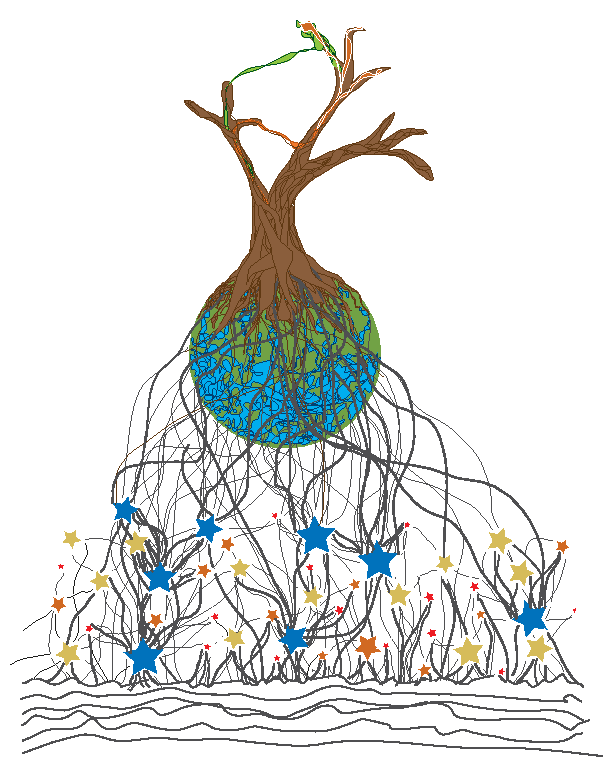
\includegraphics[width=0.6\textwidth]{gfx/front_cover} \\ \bigskip  
% \vspace{1cm}

\large \textit{A thesis submitted for the degree of \degreename}\\[0.7cm] % University requirement text
%\textit{in the}\\[0.4cm]
% \groupname\\
\deptname\\ % Research group name and department name
%\univname % University name

%{\small Draft (\today)}\\[2cm] % Date
%\includegraphics{Logo} % University/department logo - uncomment to place it


\includegraphics[width=5cm]{gfx/ANU_LOGO_cmyk_56mm}

{\normalsize September, 2022}\\[2cm] % Date
\vspace*{\fill}

\copyright Copyright by \authorname  2022

All Rights Reserved
\end{center}

\end{titlepage}

%----------------------------------------------------------------------------------------
%	DECLARATION PAGE
%----------------------------------------------------------------------------------------

\begin{declaration}
%\addchaptertocentry{\authorshipname} % Add the declaration to the table of contents
\begingroup
\large
\noindent This thesis is an account of research undertaken between January 2018 and September 2022 at the College of Engineering and Computer Sciences, The Australian National University, Canberra, Australia. 

%Except where acknowledged in the customary manner, all material presented in this dissertation including figures and photographs are original and have not been submitted in whole or part for a degree in any university.

The work presented in this thesis is that of the candidate alone, except where indicated by due literature reference and acknowledgements in the text. It has not been submitted in whole or in part for any other degree at this or any other university.

The development of ideas and research was undertaken with guidance from my primary supervisors Robert Williamson and Cheng Soon Ong, and the thesis was written by myself. The overall direction of the research was developed in collaboration with my supervisors, who also provided a lot of detailed feedback on my work along the way. The original results presented here were primarily my work.

\bigskip
\vspace{1cm}
\begin{flushright}
\authorname\\
\today
\end{flushright}
\endgroup
\end{declaration}
\vspace{3cm}
% \begingroup
% \footnotesize\emph{{Cover: Figure 1 from \fullcite{Lineweaver2012AnnRev}}}
% \endgroup
\cleardoublepage

% \begin{declaration}
% \addchaptertocentry{\authorshipname} % Add the declaration to the table of contents
% \noindent I, \authorname, declare that this thesis titled, \enquote{\ttitle} and the work presented in it are my own. I confirm that:

% \begin{itemize} 
% \item This work was done wholly or mainly while in candidature for a research degree at this University.
% \item Where any part of this thesis has previously been submitted for a degree or any other qualification at this University or any other institution, this has been clearly stated.
% \item Where I have consulted the published work of others, this is always clearly attributed.
% \item Where I have quoted from the work of others, the source is always given. With the exception of such quotations, this thesis is entirely my own work.
% \item I have acknowledged all main sources of help.
% \item Where the thesis is based on work done by myself jointly with others, I have made clear exactly what was done by others and what I have contributed myself.\\
% \end{itemize}
 
% \noindent Signed:\\
% \rule[0.5em]{25em}{0.5pt} % This prints a line for the signature
 
% \noindent Date:\\
% \rule[0.5em]{25em}{0.5pt} % This prints a line to write the date
% \end{declaration}

% \cleardoublepage

%----------------------------------------------------------------------------------------
%	QUOTATION PAGE
%----------------------------------------------------------------------------------------

% \vspace*{0.2\textheight}

% \noindent\enquote{\itshape Thanks to my solid academic training, today I can write hundreds of words on virtually any topic without possessing a shred of information, which is how I got a good job in journalism.}

% \hfill Dave Barry

%----------------------------------------------------------------------------------------
%	ACKNOWLEDGEMENTS
%----------------------------------------------------------------------------------------

\begin{acknowledgements}
\addchaptertocentry{\acknowledgementname} % Add the acknowledgements to the table of contents
\vspace{0.4cm}
\begingroup
\normalsize
The research in this thesis would not have been possible without my primary supervisors Robert Williamson, Cheng Soon Ong and Amanda Barnard. They have all been extremely patient, they have provided enormous amounts of good advice and discussion about technical details of my research, writing and about where I might be trying to go in the end and how I might get there. This research was motivated by a seemingly compelling idea about the relationship between causal models and the purpose of causal modelling, and a great deal of time was taken up with struggling to fashion this idea into a coherent and comprehensible theory. I sometimes doubted whether there was a worthwhile payoff in the end, or whether I would be able to find it. The support from my supervisors in all its forms helped me to find a path forward and to believe it was still a path worth following.

I would also like to thank Parastoo Sadeghi, Tom Everitt, Sarita Rosenstock and Zhen-Yue Chin for listening to my ideas, offering feedback, encouragement and organisational advice, and Amardeep Wander for offering flexible employment throughout much of the time I have been working on this research. Both the flexibility and the employment are deeply appreciated. I would also like to thank my parents Julie Permezel and Dennis Johnston for their help with childcare at the end of writing.

I would finally like to express my deepest gratitude to my partner, Mevlana Adil, who has gone far out of her way to support me both to commence and to finish writing this thesis through a few wild years. Without her love and support finishing would have been much less likely. I also want to acknowledge my daugher Ana\"is for her understanding and cooperation beyond my expectations for a person her age.
\endgroup
\end{acknowledgements}

%----------------------------------------------------------------------------------------
%	ABSTRACT PAGE
%----------------------------------------------------------------------------------------

\begin{abstract}
\addchaptertocentry{\abstractname} % Add the abstract to the table of contents
\begingroup
\normalsize
Mathematical formalisms of causal inference usually depend on theories of causation, and are often used to analyse problems of data-driven decision making. We show that it is possible to formalise data-driven decision problems and analyse key assumptions using a more minimal theory that aims only to satisfy the requirements of decision makers, and not to additionally offer an account of causation.

Motivated by the literature on decision theory, we consider maps from a decision maker's set of options to probability distributions on a common sample space to be the object of our study, which we call a \emph{decision model}. We extend standard probability theory to a theory of \emph{probability sets} to support reasoning with models of this type. We also make use of a string diagram notation for stochastic functions.

Drawing nontrivial conclusions from decision making models requires nontrivial assumptions. Such assumptions are usually formulated using a theory of causation. We propose that symmetries of decision models may cut out this ``causal detour''. In particular, we investigate the assumption that a sequence of pairs is related by \emph{conditionally independent and identical responses} (henceforth: CIIR sequences). We show that this assumption is equivalent to the assumption that different infinite sequences of pairs are, in a certain sense, interchangeable -- an assumption that we argue is usually unreasonable if the pairs in question are observable.

We show how causal models formulated using both the causal Bayesian network and potential outcomes approach can be represented as decision models with CIIR sequences involving latent variables. The two approaches each require a different extra assumption in order to be made compatible with ours. Causal Bayesian networks require a specification of how to ``unroll'' a structural model into a sequential model. A potential outcomes model requires a specification of how the decision maker's options relate to the rest of the model. Both approaches avoid the criticism of CIIR sequences we raise as the pairs in question are not fully observable.

The assumption of \emph{precedent} is the assumption that ``whatever we can do has been done before'', and is weaker than the assumption of CIIR sequences. We show that the assumption of precedent in conjunction with a technical condition of \emph{regular relationships between conditionals} can yield a conclusion of CIIR sequences when the data displays the right kind of conditional independence. The aforementioned technical condition is similar to a number of assumptions found in the literature that license the conclusion of a directed causal relationship from certain features of the given data. We speculate the assumption of precedent may offer an alternative way to understand directed causal relationships.
\bigskip

% \textbf{Keywords:} \keywordnames

\endgroup
\end{abstract}

%----------------------------------------------------------------------------------------
%	LIST OF CONTENTS/FIGURES/TABLES PAGES
%----------------------------------------------------------------------------------------

% \renewcommand{\listfigurename}{Figures}
% \renewcommand{\listtablename}{Tables}

\begin{spacing}{0.94} 
\tableofcontents % Prints the main table of contents
\end{spacing}

% \listoffigures % Prints the list of figures
% \listoftables % Prints the list of tables
% \listoflistings % Prints the list of python codes

%----------------------------------------------------------------------------------------
%	ABBREVIATIONS
%----------------------------------------------------------------------------------------

% \begin{abbreviations}{ll} % Include a list of abbreviations (a table of two columns)
% \textbf{ANU}&\textbf{A}ustralian \textbf{N}ational \textbf{U}niversity\\

% \end{abbreviations}

%----------------------------------------------------------------------------------------
%	PHYSICAL CONSTANTS/OTHER DEFINITIONS
%----------------------------------------------------------------------------------------

% \begin{constants}{lr@{${}={}$}l} % The list of physical constants is a three column table

% % The \SI{}{} command is provided by the siunitx package, see its documentation for instructions on how to use it

% Speed of Light & $c_{0}$ & \SI{2.99792458e8}{\meter\per\second} (exact)\\
% %Constant Name & $Symbol$ & $Constant Value$ with units\\

% \end{constants}

%----------------------------------------------------------------------------------------
%	SYMBOLS
%----------------------------------------------------------------------------------------

\begin{symbols}{ |p{0.25\linewidth}|p{0.19\linewidth}|p{0.25\linewidth}|p{0.19\linewidth}|}  % Include a list of Symbols (a three column table)
\hline
  Name & Notation & Meaning & Reference \\
 \hline
 \endhead
 \hline
 \endfoot
 \endlastfoot
  \multicolumn{4}{|l|}{\textbf{Miscellaneous symbols}}\\
 \hline
 Numbers from $m$ to $n$ & $[m,n]$ & The set of natural numbers $\{m,m+1,...,n\}$ &\\
 Numbers up to $n$ & $[n]$ & The set of natural numbers $\{1,2,...,n\}$ & \\
 Complement of $[n]$ & $[n]^{\complement}$ The set $\mathbb{N}\setminus[n]$  & \\
 Iverson bracket & $\llbracket \cdot \rrbracket$ & Function equal to 1 if $\cdot$ is true, false otherwise & \\
 Directed graphs & $\graph{G},\node{V},\node{E}$ & Directed graph $\graph{G}$, set of nodes $\node{V}$, set of edges $\node{E}$ & Definition \ref{def:dir_graph} \\
 \hline
 \addlinespace
 \multicolumn{4}{|l|}{\textbf{Probability theory}}\\
 \hline
 Variable & $\RV{X}$ & Measurable function $(\Omega,\sigalg{F})\to(X,\sigalg{X})$ & Definition \ref{def:variable} \\
 Trivial variable & $*$ & Any single-valued random variable & Definition \ref{no:single_valued} \\
 Variable sequence & $(\RV{X},\RV{Y})$ & The variable given by $\omega\mapsto (\RV{X}(\omega),\RV{Y}(\omega))$ & Definition \ref{def:seqvar}\\
 Probability measure & $\prob{P}\in \Delta(\Omega)$ & Countably additive measure on $(\Omega,\sigalg{F})$ with $\prob{P}(\Omega)=1$ & Definition \ref{def:prob_meas}\\
 Set of probability measures & $\Delta(\Omega)$ & Set of probability measures on $(\Omega,\sigalg{F})$ & Notation \ref{no:prob_meas_set}\\
 Markov kernel & $\kernel{K}:X\kto Y$ & Measurable map from $(X,\sigalg{X})$ to probability measures on $(Y,\sigalg{Y})$ & Definition \ref{def:markov_kern}\\
 Dirac measure & $\delta_x$ & Probability measure where $\delta_x(A)=1$ if $x\in A$, $0$ otherwise & Definition \ref{def:dirac_meas}\\
 Markov kernel associated with a function & $\kernel{F}_{f}$ & Markov kernel associated with $f:X\to Y$ that maps $x\mapsto \delta_{f(x)}$ & Definition \ref{def:mkern_func}\\
 Marginal distribution & $\prob{P}^{\RV{X}}$ & $\prob{P}\kernel{F}_{\RV{X}}$ & Definition \ref{def:pushforward}\\
 Conditional distribution & $\prob{P}^{\RV{Y}|\RV{X}}$ & Arbitrary Markov kernel $X\kto Y$ such that $\prob{P}^{\RV{XY}}(A\times B) = \int_A \prob{P}^{\RV{Y}|\RV{X}}(B|x)\prob{P}^{\RV{X}}(\mathrm{d}x)$ & Definition \ref{def:disint} \\
 Conditional independence & $\RV{X}\CI_{\prob{P}}\RV{Y}|\RV{Z}$ & $\prob{P}^{\RV{X}|\RV{YZ}}(A|y,z)$ does not depend on $z$ & Definition \ref{def:ci}\\
 Uniform conditional probability & $\prob{P}_A^{\RV{Y}|\RV{X}}$ & Arbitrary Markov kernel $X\kto Y$ that is a conditional distribution for every $\alpha\in A$ & Definition \ref{def:cprob_pset}\\
 Kernel product & $\kernel{K}\kernel{L}$ & The Markov kernel given by $(A|x)\mapsto \int_Y \kernel{L}(A|y)\kernel{K}(\mathrm{d}y|x)$ & Definition \ref{def:kproduct}\\
 Semidirect product & $\kernel{K}\odot \kernel{L}$ & The Markov kernel given by $(A\times B|x)\mapsto \int_A \kernel{L}(B)|y)\kernel{K}(\mathrm{d}y|x)$ & Definition \ref{def:copyproduct}\\
 Permuted sequence & $\RV{Y}_\rho$ & Given $\RV{Y}:=(\RV{Y}_i)_{i\in\mathbb{N}}$, $\RV{Y}_\rho:=(\RV{Y}_{\rho(i)})_{i\in\mathbb{N}}$ & \\
\hline
\addlinespace
\multicolumn{4}{|l|}{\textbf{String diagrams}}\\
\hline
 Identity map & $\mathrm{Id}_X$ & Markov kernel associated with the identity function $X\to X$ & Definition \ref{def:ident_k}\\
 Erase map & $\mathrm{Del}_X$, $\stopper{0.5}$ & Markov kernel associated with the trivial variable $*_X:X\to \{*\}$ & Definition \ref{def:erase}\\
 Swap map & $\mathrm{Swap}_{XY}$, $\swap{0.5}$ & Markov kernel associated with the function that swaps its inputs $(x,y)\mapsto (y,x)$ & Definition \ref{def:swap}\\
 Swap according to permuation & $\mathrm{Swap}_\rho$ & Markov kernel that swaps inputs in a manner specified by permuation $\rho$ &\\
 Copy map & $\mathrm{Copy}_{X}$, $\splitter{0.2}$ & Markov kernel associated with the function that makes two copies of its inputs & Definition \ref{def:copy}\\
\hline
\addlinespace
\multicolumn{4}{|l|}{\textbf{Probability sets and decision models}}\\
\hline
Decision model & $(\prob{P}_\cdot,(\Omega,\sigalg{F}),C)$ & An option set $C$, a sample space $(\Omega,\sigalg{F})$ and a stochastic map from options to the sample space & Definition \ref{def:dec_model}\\
Probability set & $\prob{P}_A$ & A collection of probability measures $\{\prob{P}_\alpha|\alpha\in A\}$ on a common sample space & Definition \ref{def:prob_set}\\
Option set & $C$ & Interpreted as the set of options available to a decision maker & Definition \ref{def:dec_model}\\
Nonstochastic variable & $\phi$ & Function defined on the option set $C\to A$ & Definition \ref{def:nonstoc_var}\\
Complementary variables & $(\phi,\xi)$ & Sequence of nonstochastic variables that induces an invertible function & Definition \ref{def:comp_var}\\
Extended conditional independence & $\RV{X}\CI^e_{\prob{P}_C}(\RV{Y},\phi)|(\RV{Z},\xi)$ & Generalisation of conditional independence to decision models & Definition \ref{def:eci_orig}\\
Choice variable & $\text{id}_C$ & Identity function on option set $C$; corresponds to the choice made by decision maker & \\
Tabular conditional & $\RV{Y}^X$ & Variable with the property that $\RV{Y}=\sum_{x\in X} \llbracket \RV{X}=x\rrbracket \RV{Y}^x$; not necessarily interpretable as potential outcomes & Definition \ref{def:tab_cd}\\
Input-output model & $(\prob{P}_C,\RV{D},\RV{Y})$ & Shorthand for $((\prob{P}_\cdot,(\Omega,\sigalg{F}),(C,\sigalg{C})),\RV{D},\RV{Y})$ with sequence of inputs $\RV{D}$ and corresponding outputs $\RV{Y}$ & Definition \ref{def:seq_io}\\
\hline
\end{symbols}

%----------------------------------------------------------------------------------------
%	DEDICATION
%----------------------------------------------------------------------------------------

% \dedicatory{For/Dedicated to/To my\ldots} 




%----------------------------------------------------------------------------------------
%	THESIS CONTENT - CHAPTERS
%----------------------------------------------------------------------------------------

\mainmatter % Begin numeric (1,2,3...) page numbering

\pagestyle{thesis} % Return the page headers back to the "thesis" style

% Include the chapters of the thesis as separate files from the Chapters folder
% Uncomment the lines as you write the chapters



%!TEX root = ../main.tex

\chapter{Introduction}\label{ch:introduction}

\section{Making decisions with data}

Beginning in the 1930s, a number of associations between cigarette smoking and lung cancer were established: on a population level, lung cancer rates rose rapidly alongside the prevalence of cigarette smoking. Lung cancer patients were far more likely to have a smoking history than demographically similar individuals without cancer and smokers were around 40 times as likely as demographically similar non-smokers to go on to develop lung cancer. In laboratory experiments, cells which were introduced to tobacco smoke developed ciliastasis (a slowing or stopping of the beating of cilia in the upper respiratory tract), and mice exposed to cigarette smoke tars developed tumors \citep{proctor_history_2012}. Nevertheless, until the late 1950s, substantial controversy persisted over the question of whether the available data was sufficient to establish that smoking cigarettes \emph{caused} lung cancer. Cigarette manufacturers famously argued against any possible connection \citep{oreskes_merchants_2011} and Ronald Fisher in particular argued that the available data was not enough to establish that smoking actually caused lung cancer \citep{fisher_cancer_1958}. Today, it is widely accepted that cigarettes do cause lung cancer, along with other serious conditions such as vascular disease and chronic respiratory disease \citep{world_health_organisation_tobacco_nodate,wiblin_why_2016}.

The question of a causal link between smoking and cancer is a very important one to many different people. Individuals who enjoy smoking (or think they might) may wish to avoid smoking if cigarettes pose a severe health risk, so they are interested in knowing whether or not it is so. Additionally, some may desire reassurance that their habit is not too risky, whether or not this is true. Potential and actual investors in cigarette manufacturers may see health concerns as a barrier to adoption, and also may personally want to avoid supporting products that harm many people. Like smokers, such people might have some interest in knowing the truth of this question, and a separate interest in hearing that cigarettes are not too risky, whether or not this is true. Governments and organisations with a responsibility for public health may see themselves as having responsibility to discourage smoking as much as possible if smoking is severely detrimental to health. The costs and benefits of poor decisions about smoking are large: 8 million annual deaths are attributed to cigarette-caused cancer and vascular disease in 2018 \citep{world_health_organisation_tobacco_nodate} while  global cigarette sales were estimated at US\$711 billion in 2020 \citep{noauthor_cigarettes_nodate} (a figure which might be substantially larger if cigarettes were not widely believed to be harmful).

The question of whether or not cigarette smoking causes cancer illustrates two key facts about causal questions: first, having the right answers to causal questions can underpin decisions of tremendous importance to large numbers of people. Second, confusion over causal questions can persist even when a great deal of data and and a great many facts relevant to the question are agreed upon. Understanding how the world might be influenced is often both valuable and difficult.

There are a number of different ways one could go about learning how to influence the world from data. One option is to try to obtain data that we're confident tells us directly about the consequences of the different options under consideration. For some purposes, data produced from well-conducted experiments is widely agreed to provide reliable information about the effectiveness and safety of treatments tested in the experiment. 

Alternatively, we could use the data to solve an intermediate problem, and make use of pre-existing knowledge about how to influence the world given a solution to this problem. For example, if I am on a long car trip, my tank is three quarters empty and I'm at the last fuel station for 200km, then given an answer to the question of how far my car will travel on one quarter a tank of fuel it is easy to decide whether or not I should fill up right now, and if I've logged my mileage previously I might use the data I collected to answer this question. In this example, the data don't tell me directly whether or not I should fill up. 

However, we might be in a position where, we aren't so confident that the data we can acquire can provide us with reliable guidance directly about our choice, and we don't know of any surrogate problems that make the causal question straightforward. In this case, we may want to make use of a formal theory of causal inference. When we can't see the solution immediately, a theory of causal inference can help us see more clearly the consequences of things we already know. It can also provide a language that we can use to discuss assumptions and conclusions with other people.

A lot can be said for the first two options. ``Collecting the right data'' has driven some of the most significant recent developments in algorithmic decision making. Operational advances that enable controlled experiments to be conducted at large scales have driven substantial changes in of many online businesses \citep{kohavi_surprising_2017}, and Abhijit Banerjee and Esther Duflo were recently awarded a Nobel prize in part for their pioneering role in the use of large numbers of randomised controlled trials (RCTs) to assess the effectiveness of many different development interventions in many different contexts \citep{zhang_abdul_2014}. Some fields of science have also been significantly affected by ``negative progress'' in the science of assessing experimental results. For example, in psychology in particular, replication attempts have shown that causal conclusions from experimental psychological data are less robust than many had hoped or (perhaps) believed \citep{open_science_collaboration_estimating_2015,stroebe_what_2019}. At the same time, standards for what constitutes a ``well-conducted'' experiment have risen across many fields \citep{nosek_preregistration_2018,liberati_prisma_2009}.

``Solving intermediate problems'' has also been behind tremendous technological advances. A machine that recognises your face has no useful impact in the world by itself, but there are a lot of people who know how to use such a machine for commercial or other purposes.

While a lot of progress can be made by getting around the problem that it's hard to make data-driven decisions that directly aim to influence the world, we think it is also interesting to attack the problem directly. One question we might want to ask is: \emph{why} is this problem hard? While we don't claim to know for sure, a major source of difficulty seems to come from the fact that decision making requires us to consider hypotheticals.

\subsection[Hypotheticals]{Decision making requires thinking about hypotheticals}\label{sec:assumptions}

Data driven prediction problems and data driven decision making problems can have a lot in common. The outcomes some people are interested in predicting are often outcomes other people want to influence. A forecaster might want to predict the winner of the next election, while a party strategist is interested in maximising their party's chance of victory. A product manager may be simultaneously interested in accurately inferring the sentiment expressed in reviews of their product, and in making product changes that increase the frequency that this sentiment is positive. Furthermore, data relevant to prediction is often relevant to decision making and vise-versa. Political parties often reason that electorates in which their predicted chance of victory is very low are not worth investing campaign resources in, and if a forecaster learns of evidence that one party had adopted a particularly effective election strategy they might want to revisit their prediction of the eventual election winner. The overlap is not perfect: comprehensive electorate level polls are probably more useful to the forecaster while small-scale controlled experiments are probably more useful to the strategist, but there's a lot of overlap nonetheless.

A distinguishing feature of decision making problems is that they demand the decision maker consider a collection of hypotheticals, most of which are never realised. The strategist must consider a number of different strategies to pursue, and ultimately only learns of the outcome under the strategy their party \emph{did} pursue. The election forecaster, on the other hand, can consider a number of different forecasts, but after the fact they learn exactly how accurate \emph{every} forecast was and, in particular, whether the forecast they made was better than others they could have made.

Statistical probability is well-established and widely used as a formal theory of data-driven prediction. We can speculate, on the basis of the observations above, that a formal theory of data-driven decision making may be obtained by augmenting statistical probability with the right kind of hypotheticals. In fact, even though causal inference is not quite synonymous with data-driven decision making, the most widely used theories of causal inference are theories of statistical probability augmented with a particular notion of hypothetical.

To understand the role of hypotheticals in theories of causal inference and decision making, it helps to think about the role of random variables in statistical probability. Random variables have two ``faces''; on one hand, they are defined as measurable functions whose domain is the sample space, and this allows us to reason about them using the tools of mathematics. However, they \emph{also} refer to the results of measurements conducted in the real world. This feature of random variables is not a consequence of any mathematical definition, but it is this connection to the real world that allows us to use insights derived from mathematical reasoning to inform predictions we can make about real-world events.

Hypotheticals are similarly two-faced. On the one hand, particular kinds of hypotheticals have formal definitions in theories of causal inference and decision making, and on the other hand the fact that they point to something outside the mathematical model is what allows us to use the model to help us make decisions (or to do whatever else we might want to do with a causal model). Just what it is that hypotheticals in causal models refer to is a trickier question than what random variables refer to.

\subsection{Structural interventions}

One widely-used theory of causal inference uses the term \emph{interventions} for the relevant class of hypotheticals. Interventions are defined with respect to a particular set of variables that we will call \emph{causal variables}. A graphical causal model (for the purposes of this introduction) assigns to each causal variable a possibly empty set of \emph{parents} (or causes) selected from the rest of the causal variables. Usually this assignment of parents has no cycles, but there are versions of interventional models that allow cycles \citep{bongers_theoretical_2016,forre_markov_2017}.

In this manner, the assignment of parents can be represented with a directed acyclic graph -- each causal variable is associated with a node of the graph, and an arrow $\RV{X}\rightarrow \RV{Y}$ appears in the graph just when $\RV{X}$ is a parent of $\RV{Y}$. For example, the following graph
\begin{align}
\tikzfig{simple_dag}
\end{align}
identifies three causal variables $\RV{X}$, $\RV{Y}$ and $\RV{Z}$, and identifies $\RV{X}$ and $\RV{Z}$ as parents of $\RV{Y}$, $\RV{Z}$ as a parent of $\RV{X}$ and $\RV{Y}$ as a parent of $\RV{X}$.

Given a graphical causal model and a joint probability distribution over the causal variables, an intervention on a causal variable $\RV{X}$ is formally an operation that alters the distribution of $\RV{X}$ conditional on its parents in a known way, while not affecting the distribution of any other causal variable conditional on \emph{its} parents.

Beyond the formalism of structural causal models, \emph{interventions} on $\RV{X}$ are usually taken to refer to actions that can be taken that alter the real thing represented by $\RV{X}$ in a predictable way while also avoiding directly influencing anything else (or at least, any other causal variable that appears in the model). While this sounds complicated, it can sometimes be reasonably clear what it means for an action to avoid influencing other causal variables; for example, take $\RV{Z}$ to be the last month's average rainfall, $\RV{X}$ to be the average number of flowers I see when I walk for the past month and $\RV{Y}$ to be how often I walk in the past month. In a common sense way, deciding to go for a walk today changes $\RV{Y}$ but has no effect on rainfall or flower growth. Also in a common sense way, someone else planting flowers might induce me to walk more often, but does not affect the rainfall or my inclination to walk holding weather and flowers constant. Finally, seeding clouds might cause more rainfall, which could cause more flowers and might affect my walking in an unpredictable way, but it probably doesn't alter the dependence of my walking on the weather and the scenery together. 

However, it's not always clear how to interpret interventions. A particular example that has received extended discussion is the idea of an intervention on ``obesity''. \citet{hernan_does_2008,noauthor_does_2016} have argued that ``intervention'' on obesity -- as measured by a patient's body mass index, or their weight divided by the square of their height -- are ill-defined. They note that several different actions might alter a person's body mass index, such as diet, exercise or gastric bypass surgery, and it isn't clear which of these if any count as an intervention. \citet{pearl_does_2018} responded that an intervention could be defined as an ideal action setting body mass index ``performed by nature'', although we find this idea hard to understand. 

\subsection{Potential outcomes}

The other widely used theory of causal inference uses the term \emph{potential outcomes} for its class of hypotheticals. Formally, potential outcomes are statistical random variables associated with a pair of ``ordinary'' statistical random variables. For example, if we have $\RV{X}$ again representing the mean number of flowers I see every walk and $\RV{Y}$ again representing my frequency of walks, we can define a vector of potential outcomes as a copy of $\RV{Y}$ for every possible value of $\RV{X}$: $(\RV{Y}^x)_{x\in [0,100]}$ ($\RV{X}$ is real-valued because it is a mean). 

Beyond the formalism  of the model, a potential outcome $\RV{Y}^{50}$ represents ``how often I would've taken walks last month if I had seen 50 flowers each time on average''. In cases like this, it's not clear that there is a common-sense interpretation of potential outcomes. Counterfactual statements themselves are often difficult enough to grasp that some additional theory seems needed to make sense of them.

There are some cases where potential outcomes have a somewhat easier interpretation. A version of a classic example is when $\RV{X}$ represents whether or not a patient took antibiotics and $\RV{Y}$ represents the presence of an ear infection at a follow-up appointment. In this case $\RV{Y}^0$ represents the presence of an ear infection ``had the patient not taken antibiotics'' and $\RV{Y}^1$ represents the presence of an ear infection ``had the patient taken antibiotics''. If we adopt the patient's point of view, we can view these as the consequences that the patient should consider when deciding whether or not to take the medicine.

In fact, some authors have argued that potential outcomes are underpinned by choices -- that is, we have potential outcomes $\RV{Y}^X$ precisely when $X$ is a set of options that somebody could, in principle, have chosen \citep[~pg. 4]{imbens_causal_2015}. 

In the philosophical investigation of the interpretation of counterfactuals, accounts based on structural interventions are one of the most prominent theories \citep[Section 3.3]{starr_counterfactuals_2021}, though there are several versions of this account and like all of the other theories of counterfactuals they are controversial.

\subsection{Successes of theories of causal inference}

Formal theories of causal inference exist to help us to draw reliable conclusions from data when informal reasoning isn't good enough to do so. A full account of the successes of intervention and potential outcomes based theories is beyond the scope of this introduction, but a brief overview will help to situate the work in this thesis in the broader context of causal inference theories.

\subsubsection{Successes of potential outcomes}

Potential outcomes models are characterised by the inclusion of potential outcomes variables, typically notated with superscripts $\RV{Y}^0$, $\RV{Y}^1$. These variables represent counterfactual notions -- $\RV{Y}^0$ can be read ``the value that $\RV{Y}$ would have taken, had $\RV{X}$ been 0''. The potential outcomes framework has been particularly influential in econometrics, with use of potential outcomes in that field predating the actual term ``potential outcomes''. In econometrics, and in other areas that potential outcomes have been widely used, models often involve people acting deliberately (or, sometimes, rationally) and associate potential outcomes with prospective consequences of people's choices.

\textbf{Models involving rational agents}: As we have noted, in some situations the potential outcomes $\RV{Y}^0$, $\RV{Y}^1$ and so forth look like a set of prospective consequences that a decision maker is choosing between. In some settings, we can let them be precisely that - a decision maker's expectation of the consequences of different actions they can choose. An early application of potential outcomes was to the problem of determining supply and demand curves given data on the quantity of goods exchanged and the price at which they were exchanged \citep{tinbergen1997determination,haavelmo_statistical_1943}. In this early work, a ``supply curve'' is defined as a function that maps a hypothetical price to the quantity of goods that would be supplied, were that the actual price of goods, which is for all intents and purposes a vector of potential outcomes $(\RV{Y}^x)_{x\in A}$ for some set $A$ of prices under consideration. 

Note that, in this case, ``what potential outcomes mean'' might be able to be grounded in a theory of behaviour of buyers and sellers. We can suppose that sellers are actually asking questions like ``how much would I sell if I asked for a price $x$?'' and getting hints about the answer from buyers and other sellers. Under some idealisations -- for example, maybe we require the buyers and sellers to all agree on questions of this nature -- we might be able to consider the potential outcomes to represent the the traders' answers to these questions.

\textbf{Analysis of randomised experiments:} The potential outcomes framework offers an account of what it is that a randomised experiment achieves so that it enables causal conclusions to be drawn. Under this framework, the critical condition is the statistical independence of the input $\RV{X}$ from the vector of potential outcomes $(\RV{Y}^x)_{x\in X}$ (in the potential outcomes framework, $\RV{X}$ is often called an \emph{assignment}). If the value of $\RV{X}$ is completely determined by some physical randomisation procedure then (so the argument goes) it must be independent of the potential outcomes. 

A more general kind of randomised experiment completely determines the values of inputs based on a collection of other variables $\RV{W}$ called \emph{covariates} and some physical randomisation procedure. In this kind of experiment, the inputs are independent of the potential outcomes conditional on the covariates. When this holds, the inputs $\RV{X}$ depend probabilistically on the covariates $\RV{W}$, and this dependence is usually called the \emph{assignment mechanism}. When this dependence is known or able to be estimated, it can facilitate the calculation of many causal effects of interest (see Section \ref{sec:potential_outcomes} for more details). Using the potential outcomes framework, many techniques have been developed to estimate the assignment mechanism and to estimate causal quantities of interest given the assignment mechanism -- for example, many methods and worked examples can be found in \citep{imbens_causal_2015}.

Because the potential outcomes framework doesn't offer a theory of counterfactuals, it doesn't come with an explanation of why the inputs are independent of the potential outcomes in a randomised experiment -- this is a matter that stands outside the formal theory. One could consider an explanation that goes something like: we imagine the potential outcomes to be fixed at the time that the inputs are decided, so the inputs have no influence over them. Furthermore, if the inputs are physically randomised, the potential outcomes can have no influence over the inputs, and so the two are independent. We might also consider the converse of this claim: perhaps any reasonable theory of counterfactuals must yield the conclusion that potential outcomes are (statistically) independent of any physically randomised inputs.

Unlike the case of supply and demand, the deliberate action in a randomised experiment is the assignment carried out by the experimenter rather than the choices made by subjects of the model.

\textbf{Subpopulations with different behaviour:} Rather than having an input $\RV{X}$ that is completely determined by a physical randomization mechanism, sometimes experiments of interest have some physically randomized $\RV{Z}$ that influences but does not fully determine $\RV{X}$. For example, if $\RV{X}$ records whether or not someone took a medicine, $\RV{Z}$ might record whether or not the medicine was prescribed. Experimenters might be able to have prescriptions randomized, but not the actual act of taking the medicine. The potential outcomes framework first offers us a way to understand that this is not analogous to an experiment where $\RV{X}$ is randomised: by application of probability theory, the fact that the potential outcomes are independent of $\RV{Z}$ does not mean that they are independent of $\RV{X}$.

A notable result proven using the potential outcomes framework is that, under an assumption that prescribing a medicing never induces anyone to avoid the medicine who would otherwise have taken it (``no defiers''), it is possible to determine the effect of taking the medicine on the subpopulation of ``compliers'' -- people who were induced by the prescription to switch from not taking the medicine to taking it. See \citep{imbens_identification_1994} for more details.

In this setting, there are often deliberate choices carried out by the experimenter -- namely, the assignment of $\RV{Z}$ -- and also deliberate choices carried out by experimental subjects -- the choice of $\RV{X}$.

\subsubsection{Successes of structural interventional models}

Structural interventional models feature a collection of causal variables, and each variable is assigned a set of parents from the remaining causal variables. Each causal variable may be intervened on, which in general alters the distribution of the variable conditional on its parents while not changing the distribution of any other causal variable conditional on that variable's parents.

\textbf{A formal theory of directed causal relationships:} A point that is repeatedly made by \citet{pearl_causality:_2009} and \citet{pearl_book_2018} is that informal notions of causal relationships play a key role in the formulation of many statistical models. For example, in the account of randomised experiments above, we said that the treatment assignment was ``determined by'' a physically random procedure. This statement is not backed by a formal theory, but the relation invoked by the phrase ``determined by'' is something like a causal relationship. It implies that the treatment assignment and the output of the randomisation are deterministically related, but ``being determined by something'' is not a symmetric relationship.

Structural interventional models offer a theory of causal relationships that aims to clarify these intuitions. They have been used to analyse questions like ``what is the likelihood that the medicine caused the reaction?'' (\citet[ch. ~9]{pearl_causality:_2009}, \citet{pearl_causes_2015}), which differ from traditional causal inference questions that are more focused on the consequences of actions than on attributing responsibility. 

The question of whether the structural interventional account explains causal intuitions has been taken on by philosophers (see, for example, \citet{woodward_causation_2016}), but whether it is successful in doing so is contested \citep{cartwright_modularity_2001}.

Interventions might not be the \emph{only} possible way to ground intuitions about directed causal relationships. An alternative proposition is that the distribution of a causes and the distribution of an effect conditional on the distribution of a cause should be \emph{algorithmically independent}, or that the relation between them should be \emph{generic} \citep{lemeire_replacing_2013}. Because this principle can induce directed relationships between pairs of variables, it can potentially offer an account of directed causal relationships without appealing to interventions, though it has been substantially less studied than the structural intervention account of directed relationships. However, unlike the interventional theory, this does not seem to tell us how causal relationships should inform our ideas of the consequences of taking an action\footnote{Throughout this thesis, we use the term ``intervention'' to refer to an operation defined in the structural interventional account of causal inference, or the interpretation of this operation. We use the word ``action'' to refer to something that may or may not be interpretable as an intervention.}.

One of the contributions of the present work is Theorem \ref{th:det_obs_to_cons} in Section \ref{sec:precedent}, which shows that under an assumption of generic relationships between the conditional distributions of causes and effects together with the assumption that a proposed plan of action has a precedent then conditional independences in observed data can imply certain relationships do not change under any action the decision maker might take. Invariant relationships under action, which are taken to be axiomatic in the theory of structural interventions, can be shown to follow from the assumption of generic relationships between conditional distributions and the previously mentioned assumption that actions are precedented. We think this suggests that it may be possible to forge a unified view of directed causal relationships that subsumes both the notion that causal relationships should be invariant under action and the notion that conditional distributions should be generically related in the causal direction, although precisely how to do this is an open question.

\textbf{Causal inference under generic assumptions:} Traditionally, analysis of causal inference problems involves certain non-generic assumptions like the assumption of independence of inputs and potential outcomes. These assumptions are non-generic because they do not apply to arbitrary causal inference problems, and so the analysis made under these assumptions can only be applied to data generated in particular contexts (for example, in controlled experiments).

The structural models tradition, however, has fostered the analysis of \emph{causal discovery}, which is the problem of learning causal relationships from data which may not be known to satisfy certain strong assumptions. There are two main approaches to causal discovery: conditional independence-based causal discovery infers a family of causal graphs from conditional independences inferred from a dataset, while the previously mentioned theory that conditionally probabilities should be algorithmically independent in the causal direction has led to a wide variety of different approaches for discovering the direction of causation. Early examples of conditional independence based inference are the PC algorithm and the Causal Inference Algorithm \citep[Ch. 5\& 6]{spirtes_causation_1993} and Greedy Equivalent Search \citep{chickering_optimal_2003,chickering_learning_2002}, while more recently it has been discovered that the problem of searching for a graph satisfying inferred conditional independences can be posed as a continuous optimization problem \citep{zheng_dags_2018,ng_graph_2019}. Examples of the applications of the idea of algorithmic independence include methods based on the assumption of additive noise \citep{hoyer_nonlinear_2009,shimizu_linear_2006} and so-called \emph{information geometric causal inference} (IGCI) methods \citep{daniusis_inferring_2012}. Reviews of these methods can be found in \citep[ch. 4, 5, 6 \& 7]{peters_elements_2017} and \citep{mooij_j.m._distinguishing_2016}.

While the aim of this analysis is to discover causal relationships from generic data, in practice the key assumptions are not completely generic. \citet{uhler_geometry_2013} examined how frequently the key assumption of $\lambda$\emph{-faithfulness} underpinning the conditional independence based approach is violated, and finds that (under their assumptions) models with more than 10 variables and relatively dense causal connections almost always violate the condition. Owing to the fact that algorithmic independence is incomputable and suitable approximations have to be found for practical algorithms, the algorithmic independence based approach has typically involved special conditions like linear causal relationships with non-Gaussian additive noise.

\textbf{Causal identification in complex models:} Potential outcomes approaches have proposed a wide variety of sufficient assumptions for estimating causal effects, but there are models in which causal effects can be estimated that are typically ignored by the potential outcomes approach. The graphical models community usually separates the problem of \emph{identification} and \emph{estimation}; a causal effect is \emph{identified} if it can be computed from the joint probability of the observed variables. If this is possible, then the causal effect could in principle be calculated from an estimate of the joint probability (though estimating the entire joint probability is usually more than is needed). 

One of the simplest graphical models in which causal effects are identified that haven't received much attention in the potential outcomes literature is the ``front-door'' condition. Given a graphical model for which it is impossible to identify the effect of $\RV{X}$ on $\RV{Y}$, but the effect of $\RV{X}$ on $\RV{W}$ and the effect of $\RV{W}$ on $\RV{Y}$ can be separately identified, then it is possible to compose the two to identify the effect of $\RV{X}$ on $\RV{Y}$ \citep[Section 3.3.2]{pearl_causality:_2009}. In fact, a complete characterisation of the identifiability of graphical models has been given by \citet{shpitser_complete_2008}, and a more recent alternative characterisation is presented in \citet{richardson_nested_2017}.   

\subsection{Challenges to popular theories of causal inference}

Despite the fact that both the potential outcomes and structural interventional approaches have substantially advanced everyone's understanding of causal inference, we believe that both approaches face difficulties that make them hard to apply outside of special settings. The difficulty with potential outcomes is easy to state: the potential outcomes framework offers no clear theory of counterfactuals. Thus the appropriate interpretation of counterfactuals statements must either be obvious or established by convention or else communication using the framework risks confusion. 

As we noted earlier, some authors have suggested that potential outcomes should represent the potential consequences of choices or actions, and that this might perhaps form the basis of a theory of counterfacutals. The work in this thesis builds a theory of causal inference starting from the view that the fundamental problem to be addressed is a problem of making informed choices. We don't have a particularly strong view on whether our theory is fundamentally different to potential outcomes, or whether the two approaches are fundamentally similar but look different because we focus on modelling an abstract problem of making informed choices, while potential outcomes is often focused much more on various concrete problems.

Alternatively, some authors have argued that the theory of structural interventions is the appropriate theory of counterfactuals for potential outcomes \citep[chap. ~7]{pearl_causality:_2009}. In this case, the following remarks on structural interventional theories apply.

\subsubsection{Difficulties for structural models}

If a decision maker has a sound informal understanding of causal relationships relevant to their problem, structural models are often an excellent tool to formalise this understanding and derive conclusions from it. However, if a decision maker is dealing with a problem where he does \emph{not} have a sound informal understanding of causal relationships, what does the structural approach offer him? The structural model community might suggest that he performs \emph{causal discovery}; this is some procedure that takes his data and offers him a best guess of the structural model associated with this data.

What role should this learned structural model play in the decision maker's subsequent deliberation? We propose three answers to this question:
\begin{enumerate}
    \item The structural model tells the decision maker what his options are and what their consequences are.
    \item The structural model can be combined with the decision maker's prior knowledge of what his options are to offer an assessment of their consequences.
    \item The structural model and the decision maker's options coevolve; perhaps the decision maker has an initial idea of what his options are which motivates a particular avenue of causal discovery which, in turn, migh prompt the decision maker to reevaluate his options and so forth.
\end{enumerate}

We consider the second and third answers reasonable, though the third answer is beyond the scope of this thesis. However, these two answers seem to be in tension with typical practice in causal discovery. Causal discovery algorithms typically take only the given data as input, and depend in no way on any specification of the decision maker's options. Despite this, whether or not a structural model can offer an assessment of the consequences of a set of options is sensitive to the options under consideration.

\begin{example}[Different sets of options require different models]\label{ex:prob_int_2}
Suppose on day $i$, at some point during the day, a volunteer Ella looks at the current outside temperature and logs whether it is ``cold'' or ``hot'' as $\RV{T}_i$, whether or not she's wearing a jumper as $\RV{X}_i$ and whether she feels cold, comfortable or hot as $\RV{Y}_i$. Under normal circumstances, in cold weather she usually wears a jumper and feels comfortable, and in hot weather she wears no jumper and feels comfortable. If she is uncharacteristically not wearing a jumper on cold days, she feels cold, and if she is wearing one on hot days she feels hot.

Suppose she's asked to wear her jumper no matter what. In this case, she will feel comfortable on cold days as before, and will feel hot on hot days also as before. Under this ``intervention'', the relationship between her perceived body temperature and the joint specification of her clothing and the weather is unchanged. If we assume an acyclic structural model, that the instruction to wear a jumper should indeed be modeled by an intervention in this model, and that the temperature may be a cause but not an effect of body temperature and jumper wearing, then we can conclude from the results of the intervention that jumper wearing causes body temperature perception and that this relationship is unconfounded given the daily temperature:
\begin{align}
    \tikzfig{simple_dag_jumper}\label{ex:simple_dag_jumper}
\end{align}

Suppose we \emph{also} want to consider the effect of actions affecting Ella's perceived body temperature. We could ask her to exercise intensely before filling out the survey on some days. What we find is, because exercise raises her body temperature, after exercising she feels comfortable with no jumper in cold weather and feels hot in hot weather with no jumper. However, we \emph{also} find that she now prefers not to wear a jumper in cold weather. This finding does \emph{not} correspond to the structural model \eqref{ex:simple_dag_jumper}.

The following modification to this structure also does not yield the desired result:
\begin{align}
    \tikzfig{simple_dag_jumper_bd}
\end{align}
Under normal circumstances, the condition $\RV{Y}_i=\text{``feel hot''}$ always happened when Ella was wearing a jumper, but under the exercise condition it corresponds to no jumper wearing. Thus the conditional distribution of $\RV{X}_i$ given $\RV{T}_i$ and $\RV{Y}_i$ is not the same in the exercise condition to the normal condition.

If we introduce a new unobserved variable $\RV{Y}^X$ that represents Ella's beliefs about how she would feel if she were or were not to wear a jumper, then the following structural model can yield the desired result for both interventions (note: there are also other possibilities):
\begin{align}
    \tikzfig{not_simple_dag_jumper}\label{ex:not_simple_dag}
\end{align}

Here, we say that Ella's beliefs about her perceived body temperature are influenced by the outside temperature, whether or not she's wearing a jumper and her actual perceived body temperature. Here, once again, her perceived temperature is caused only by $\RV{T}_i$ and $\RV{X}_i$, which reproduces the fact that her perceived temperature depends on these variables in exactly the same way after intervention on her jumper wearing. However, the only cause of her jumper wearing is her beliefs about how comfortable she will feel with a jumper on, which can be influenced by interventions on her body temperature. Thus this model can also reproduce the assumed fact that when her body temperature is intervened on, she acts to maintain a comfortable equilibrium.

Concretely, taking $-1$ to be ``cold'', $0$ to be ``comfortable'', $1$ to be ``hot'', $0$ also for ``no jumper'' and $1$ for ``jumper'', we specify the model as
\begin{align}
    \RV{T}_i &\sim U(\{-1,0\})\\
    \RV{Y}^X_i &\leftarrowtriangle \begin{cases}
                                x\mapsto x-1 & \text{ if } \RV{Y}_i = \RV{X}_i -1\\
                                x\mapsto x & \text{ if } \RV{Y}_i = \RV{X}_i\\
                                x\mapsto 1 & \text{ if } \RV{Y}_i = \RV{X}_i+1
                            \end{cases}\\
    \RV{X}_i &\leftarrowtriangle \begin{cases}
                    1 &\text{ if }\RV{Y}^X_i=x\mapsto x-1\\
                    0 &\text{ otherwise}
    \end{cases}\label{eq:struct_x}\\
    \RV{Y}_i &\leftarrowtriangle \RV{T}_i + \RV{X}_i\label{eq:struct_y}
\end{align}
Here, a left arrow indicates a causal assignment. This has a unique solution for each value of $\RV{T}_i$. Instructing Ella to wear a jumper is modelled by replacing the right hand side of Eq. \eqref{eq:struct_x} with 1 and instructing Ella to exerciese is modelled by replacing the right hand side of  Eq. \eqref{eq:struct_y} with $\text{max}(1,\RV{T}_i + \RV{X}_i + 1)$. See \citep{bongers_theoretical_2016,forre_causal_2020} for a much more in-depth treatment of structural models with cycles, and see \citep{eberhardt_combining_2010,ghassami_causal_2020} for algorithms for discovering linear cyclic causal structures

Suppose, finally, we are interested in the results of a) tampering with the device Ella uses to determine the temperature each day and b) putting up a large structure to shade Ella's house. Both of these actions are likely to affect the reading $\RV{T}_i$, but otherwise have different consequences. It does not seem possible, therefore, that any single structural model limited to the variables $\RV{X}_i$, $\RV{Y}_i$ and $\RV{T}_i$ and functions thereof can represent the consequences of both of these actions.
\end{example}

In this example, different kinds of models are suitable for assessing the consequences of different sets of options, and a model accommodating all of the options considered is substantially more complex than a model accommodating only the request to wear a jumper. Maybe it is in principle possible to come up with a structural model that covers every set of options anyone might want to consider -- though it's far from obvious that this really is possible -- but it would be very surprising to us if there was any practical way to do so.

Practically, there seems to be some tension between the views that structural models should prescribe exactly what can be done and the view that they should be flexible enough to accommodate a decision maker's needs. For example, we can find in the literature a wide variety of types of intervention that can be considered alongside structural models: beyond the standard ``perfect interventions'' \citep[ch. ~1]{pearl_causality:_2009,hauser_characterization_2012} we have soft interventions \citep{correa_calculus_2020,eberhardt_interventions_2007}, general or fat-hand interventions \citep{eberhardt_interventions_2007,yang_characterizing_2018,glymour_evaluating_2017} and general interventions with unknown targets \citep{brouillard_differentiable_2020}. Offering such a variety of different kinds of interventions seems to acknowledge that decision makers need some flexibility to specify structural models that will suit their needs.

On the other hand, evaulation of causal discovery research almost invariably employs a measure that does not depend on any set of options under consideration at all -- as in the structural hamming distance, which counts the number of edges that differ between an inferred structure and a putative ``true'' structure -- or that assumes that options are given by perfect interventions with respect to the true structure, as in the structural intervention distance \citep{peters_structural_2015}. To offer just a few examples, \citep{brouillard_differentiable_2020,scherrer_learning_2022,toth_active_2022,forre_constraint-based_2018,chickering_optimal_2003,ng_graph_2019,zheng_dags_2018,spirtes_causation_1993} all evaluate their methods according to one or both of these kinds of measures.

Why do we have on the one hand an acknowledgement of the need to allow ``interventions'' in structural models to be flexible enough to accommodate a decision maker's needs, while on the other hand causal discovery methods are evaluated only according to a rigid interpretation of perfect interventions? One of the reasons for this, we presume, is that if we consider a very broad class of interventions -- say, general interventions with unknown targets -- then a structural model places no constraints on what consequences can be achieved by an arbitrary intervention. However, we want causal discovery to tell us something useful, and restricting our attention to what it tells us about perfect interventions ensures that at least it tells us something nontrivial. Exactly when this is also something useful, we don't know.

In short, there is some conceptual difficulty for structural models in determining how they should interface with a given decision maker's options. In this thesis, we ask (loosely speaking) the reverse of this question; rather than starting with a structural model and asking how we can accommodate a decision maker, we start with a decision maker and ask what sorts of models they might want to use.

\section{Outlining our approach}

As we have noted, decision making requires the consideration of a collection of hypotheticals -- specifically, a decision maker must consider the options she has available, and specifically wants to consider the consequences of choosing each of these options. Our approach is to suppose that our job is to help a decision maker evaluate their options. This is an idealisation; a lot of causal analysis doesn't end up directly making a decision, but it might help a third party's decisions in ways the analyst may or may not anticipate. However, it's a different idealisation to the frameworks discussed above. Potential outcomes depend on certain counterfactual statements, structural models depend on ideal interventions and our approach depends on a decision maker's set of options. However, decision making is often at least indirectly the aim of causal inference, and decision problems require the decision maker to consider a set of options, while they do not require a decision to consider counterfactuals or interventions. 

This approach, which can be called a \emph{decision theoretic approach to casual inference}, has previously been explored by \citet{heckerman_decision-theoretic_1995} as well as \citet{dawid_causal_2000,dawid_influence_2002,dawid_decision-theoretic_2012,dawid_decision-theoretic_2020}. Our approach builds on this earlier work, with a particular focus on the way assumptions of symmetry or regularity in sequential decision problems can lead to models that support non-trivial inferences from data.

To a decision maker, our approach offers the possibility of analysing their problem with fewer assumptions. The two approaches surveyed above require a decision maker who wishes to formally pose their problem to accept a set of options to consider, probability theory, an account of causal effects (whether structural or some other kind of counterfactual) and some ``bridging'' assumption that links their options to the causal effects. In contrast, we only require them to accept a set of options and probability theory. In either case, the decision maker will also have to make additional assumptions that reflect their best guesses about how to use their available data to make a good choice. A key question is whether this approach facilitates solutions to practical decision making problems with assumptions that differ from those that must be made under the existing widely used frameworks.

A basic condition that corresponds approximately to unconfoundedness in standard causal analysis is the assumption of \emph{conditionally independent and identical responses}. In the spirit of De Finetti's analysis of conditionally independent and identically distributed sequences, we examine in Chapter \ref{ch:evaluating_decisions} the relationship between conditionally independent and identical responses and symmetries of a decision making model. This offers an alternative means of analysing assumptions of unconfoundedness in terms of the interchangeability of different datasets. The basic idea here is, instead of making assumptions about which structural causal relationships hold or how counterfactual quantities are distributed, we phrase assumptions in terms of which experiments are essentially identical. For example, the assumption that the \emph{response functions} in a model of a combined sequence of observational and experimental data are identical, we show, is equivalent to the assumption that collecting only the observational data is essentially identical to collecting only the experimental data. We regard this as a mostly negative result; for most decision problems, a precise assumption of identical response functions is usually untenable, though it may be tenable in some approximate form.

The established approaches to causal inference have received a great deal of cumulative development effort, and many specific applications have already been studied. In Chapter \ref{ch:other_causal_frameworks}, we show how to represent Causal Bayesian Networks (a kind of structural causal model) and Potential Outcomes models as decision making models. In particular, we show how each framework by default leaves complementary pieces of a model underspecified. Causal Bayesian Networks are, by default, non-sequential and so one must specify how they can be ``unrolled'' into a sequence model in order to use them to model a decision problem. Potential outcomes models are sequential, but do not provide an unambiguous way to include the options available to the decision maker into the model. Because we can perform this translation, this means that it's possible in principle to translate established application specific reasoning to our framework.

The results from Chapter \ref{ch:evaluating_decisions} are mostly negative in their practical relevance -- certain assumptions that would make inference from data possible are usually untenable. In Chapter \ref{ch:other_causal_frameworks} we explore the weaker assumption of \emph{precedent} (``whatever I can do, it's been done by somebody before''). We prove Theorem \ref{th:det_obs_to_cons}, which establishes that, subject to the additional assumption of \emph{generic probabilistic relations between conditionals}, one can conclude from a conditional independence in observed data that there is a corresponding invariant relationship among the consequences of every option available to the decision maker. 

In the structural models literature generic probabilistic relations between conditionals have been used as an assumption to justify the inference of directed causal relationships. A classic result from \citet{meek_strong_1995} establishes that an assumption of generic probabilistic relations between conditionals ``in the causal direction'' can support the assumption of \emph{faithfulness}, which facilitates the inference of structural models from conditional independences in observed data. An observation subsequently made by a number of authors, for example \citet{lemeire_replacing_2013}, is that these kinds of generic relationships often intuitively hold in the causal direction, and can be violated in the countercausal direction. We use the same idea of generic relationships between conditionals, but by making the assumption of precedent we can skip many steps of reasoning. To use the assumption of generic relationships between conditionals to infer the consequences of choosing different options, a structural modeller needs to infer the causal structure, assume sufficiency (or some other assumption strong enough to support structural identifiability) and then make additional assumptions to connect the intervention operations in the structural model back to the actual options under consideration. With our result, a decision maker can make a similar assumption of generic relationships between conditionals, assume that the consequences of their choices have precedent, and immediately conclude from an observed conditional independence that an observed relationship is invariant over their actual options at hand. Furthermore, we argue in Section \ref{sec:precedent} that an assumption similar to the assumption of precedent is very often built into structural models.

In Theorem \ref{th:det_obs_to_cons}, we assume generic relationships between the key conditional distributions. There is a large literature on methods to identify ``generic relationships'' between conditional probabilities in order to infer causal directions. An open question is whether these methods provide evidence the right kind of ``genericity'' for the application of Theorem \ref{th:det_obs_to_cons}.

In Chapter \ref{ch:other_causal_frameworks} we also examine symmetries of experiments that support a judgement of independent and identical response functions. We begin with an assumption of \emph{individual-level response functions}, reminiscent of the potential outcomes model construction, except each ``potential outcome'' is associated with a unique identifier. We then show that under the assumptions of permutability of identifiers and full control over the inputs, the input-output relations are given by conditionally independent and identical response functions. This result differs from standard accounts of causal identification in controlled experiments in that we connect the required assumptions to symmetries of experiments that might be performed.

Chapters \ref{ch:tech_prereq} and \ref{ch:2p_statmodels} provide context and prerequisites for the work that follows. In particular, causal inference theories aren't the only theories that address decision making algorithms. These questions are also addressed by the fields of reinforcement learning, optimal control and statistical decision theory (and, no doubt, others besides). One distinction we can draw between these fields and the field of causal inference is that a key difficulty in causal inference problems is just how to relate consequences of actions to observations. In reinforcement learning, an \emph{environment} is typically assumed that represents the ``ground truth'' of consequences of actions, and the history of consequences can be used to infer which environment an agent is operating in \citep{barto_reinforcement_1998}. While optimal control is such a large field it's inappropriate to make any sweeping generalisations, basic versions of control theory assume a \emph{system model} is available that maps states and inputs to updated states and outputs \citep{ogata_discrete-time_1995}. Finally, in statistical decision theory the relevant notion of consequences of actions is given by the \emph{state} and the \emph{loss}, which like the environment in reinforcement learning, are basic elements of the problem \citep{wald_statistical_1950}.

There is substantial overlap between these different methods for relating observations to consequences. For example, \citet[Chap.~4]{lattimore_learning_2017} shows how the environment model in a reinforcement learning problem can be specified using a causal graphical model. In Chapter \ref{ch:2p_statmodels} we survey the literature on modelling decision problems, and show that many different decision theories posit that decision models, including \emph{evidential decision theory} and \emph{causal decision theory} share the same basic type. We also show how a particular class of decision making models -- a class that contains the models investigated in all subsequent chapters -- a classical statistical decision problem.

The mathematical basis for essentially all of the work in this thesis is probability theory, though we make use of nonstandard constructions within the theory to facilitate the representation of sets of options in the models we consider. We introduce the relevant theory in Chapter \ref{ch:tech_prereq}. As is common in causal inference, we often use a graphical language to represent probabilistic decision models. The language we use is somewhat different to the directed graphs that are standard in the area. We use a string diagram notation that can be related to ordinary directed graphs as in \citep{fong_causal_2013}, but also supports equality statements and a collection of transformations that can be applied to a diagram to yield an equivalent diagram.

We conclude in Chapter \ref{ch:discussion}, revisiting key results from this thesis and surveying important questions that they raise.

% These assumptions all invoke either ``potential outcomes'' or ``causal structure''. Potential outcomes are, by definition, the union of a set of observed variables and a set of hypothetical claims. If one is inclined to accept that causal structures are ultimately underwritten by certain experimental procedures, then causal structures may be observed under some conditions (for example, if an experimental procedure is given for each $do()$-intervention, one can apply the method of \citep{eberhardt_almost_2008}) However, causal structures are often held to represent relationships that cannot be reasonably probed by an experiment (\citep[Chap. ~11]{pearl_causality:_2009},\citet{pearl_does_2018}), and in our view the general question of whether causal structures are observable or a mixture of observable properties and hypothetical claims is unresolved.

% Decision making must entertain some hypothetical statements. As has been pointed out above, a decision maker must consider multiple options and their likely consequences, and select from among the options. The proposition ``the consequences of $\alpha$ are better than the consequences of $\alpha'$'' is a hypothetical one: the decision maker ultimately chooses only one of $\alpha$ or $\alpha'$, and usually cannot ever verify that the chosen option really is better than the alternative. However, the hypotheticals that the assumptions above ask us to entertain do not on the face of it seem necessary to compare different options like this. The hypothetical part of potential outcomes doesn't refer to possible consequences of choices but to hypotheticals that have (in some sense) ``already happened'' by the time the data is reviewed. An identifiable causal structure may have many implications besides those that are necessary to make a choice in the decision problem at hand.

% Assumptions with mixtures of hypothetical and real implications are difficult to evaluate. On the one hand, the fact that they have real implications means that one cannot simply accept anything, while on the other hand the fact that some implications are hypothetical means that it can be difficult to form a clear picture of how the world actually differs depending on whether the assumption is true or false.

% % Without going into detail about any of these assumptions, we propose that none of them are presently suitable for ``mass production'' in the way that controlled experiments are. To take one example, even though \citet{lee_randomized_2008} writes of the regression discontinuity assumption ``it is shown below that causal inferences from RD designs can sometimes be as credible as those drawn from a randomized experiment.'', there is a lively debate about the applicability of this method just to the specific case of US House of Representatives elections \citep{snyder_detecting_2005,grimmer_are_nodate,caughey_elections_2017,cuesta_misunderstandings_2016}, which is the example \citet{lee_randomized_2008} used to illustrate his argument in the first place. The amount of careful case-by case attention required to assess these assumptions seems to make it harder to use them in large-scale data-driven decision making in a manner analogous to the results of controlled experiments or predictive models. 

% In brief:
% \begin{itemize}
%     \item Decision making algorithms require stronger assumptions than predictive algorithms
%     \item These assumptions are often particularly hard to evaluate
% \end{itemize} 

% \section{Exploring alternative foundations}

% The development of decision making algorithms is constrained by the assumptions we can make. Such problems are often addressed using theories of causal inference. Theories of causal inference allow us to state assumptions precisely, to understand them in various different ways so that we can better apply our informal means of evaluating them and, hopefully, to make sound choices about whether to accept an assumption or not. A number of such theories exist, and we can distinguish three traditions with wide adoption in different fields: causal Bayesian networks, potential outcomes and structural equation models. These are described in more detail in Chapter \ref{ch:other_causal_frameworks}.

% This thesis explores an alternative theory of algorithmic decision making. Our starting point is the observation in Section \ref{sec:assumptions} above that decision making problems call on a decision maker to compare a number of different options on the basis of their consequences. The conclusion is that, to construct a decision making model, where in classical statistics we might consider a probability distribution $\prob{P}$ defined on a sample space $(\Omega,\sigalg{F})$, we instead consider a function from the set of options $C$ to probability distributions on a sample space: $\prob{P}_\cdot:C\kto \Omega$. This extension of the basic statistical model is what underpins this entire thesis.

%  One might ask us all: if we already have three ways to theorise about this problem, why do we need a fourth? To a large extent, for questions like these, the proof is in the pudding -- do the alternative foundations offer insights that are hard to see from other points of view? However, we think that even before learning what alternatives can deliver, there are reasons to believe they are worth exploring.

% A broad reason for paying special attention to theoretical foundations in causal inference is outlined in Section \ref{sec:assumptions}: causal inference typically requires assumptions that are strong and particularly hard to evaluate. Alternative theoretical foundations can yield alternative perspectives on old assumptions and suggest new assumptions that accomplish desired goals. For these reasons, causal inference is a field that merits particular attention to foundations. In fact, the reason we have several different causal inference traditions is because different researchers have, at different times, attacked the problem of how to formulate causal models in different ways. This project has been fruitful -- it has facilitated the entire field of research into causal inference. In addition to the handful of identification results suggested above, some other insights enabled by these projects are:
% \begin{itemize}
%     \item With potential outcomes, it is possible to offer a precise formal statement of what it is that controlled experiments should achieve -- \emph{strong ignorability} \citep{rubin_causal_2005}
%     \item With potential outcomes we can precisely express the notion of ``the effect of a choice on the people whose behaviour changed on account of that choice'', formalised as the \emph{local average treatment effect} \citep{imbens_identification_1994}
%     \item[-] There is a close correspondence between the intuitive idea of directed causal relationships between variables and the factorisation of joint probability distributions, formalised as the \emph{causal Markov condition} (\citet[Chap. ~1]{pearl_causality:_2009},\citet{wright_method_1934})
%     \begin{itemize}
%         \item Particular credit is due Pearl for pointing out how common it is for researchers to smuggle these ``intuitive causal ideas'' into discussions with no accompanying theory of causation - see for example \citet[pg. 96]{pearl_causality:_2009}
%     \end{itemize}
%     \item[-] The field of conditional-independence based \emph{causal discovery} \citet{spirtes_causation_1993}
%     \item[-] The field of causal discovery based on the \emph{independence of cause and mechanism} \citet{scholkopf_causality_2022}
%     \item[-] Causal identification in semi-Markovian models \citet{shpitser_complete_2008}
% \end{itemize}

% Here, items marked with a dot are (in our view) difficult to formulate using causal graphical models alone, while items marked with a dash are (again, in our view) difficult to understand from the potential outcomes perspective.

% We have some specific reasons for wanting to go beyond these two frameworks. For the potential outcomes framework, the reason is quite simple: in order to make a decision, we must consider a map from some set of options $C$ to distributions over consequences, and the potential outcomes framework does not provide such a function at the base level. Once we incorporate such a function, it is not clear that there is any longer a need for potential outcomes at the axiomatic level (though it may still be possible to define variables in particular problems that play a similar role).

% The situation with causal graphical models -- that typically do have a notion of intervention -- requires some more explanation. Causal graphical models are characterised by sets of variables with directed relationships between them, and these directed relationships are underwritten by the idea of \emph{interventions}. Our suspicion is that this kind of model describes a special case of the kind of model we investigate -- which, recall, is defined by a function from a set of options $C$ to a set of probability distributions over a fixed sample space -- but is not appropriate to describe the general case. The issue centres on variables and interventions.

% First, it is important to point out that while interventions are suggestively named, they are not defined as ``things an experimenter actually goes and does''. Any identification of actions that can be taken with interventions is up to the analyst's discretion for a particular problem. 





% \section{Theories of causal inference}



% For causal questions that are controversial or difficult, it is tremendously advantageous to be able to address them transparently. Theories of causation enable this; given a theory of causation and a set of assumptions, if anyone claims that some conclusion follows it is publicly verifiable whether or not it actually does so. If the deduction is correct, then any remaining disagreement must be in the assumptions or in the theory. For people who are interested in understanding what is true, pinpointing disagreement can be enlightening. Someone could learn, for example, that there are assumptions that they find plausible that permit conclusions they did not initially believe. Alternatively, if a motivated conclusion follows only from implausible assumptions, hearing these assumptions explicitly might make the conclusion less attractive. 

% Theories of causation help us to answer causal questions, which means that before we have any theory, we already have causal questions we want to answer. If potential outcomes notation and causal graphical models had never been invented there would still be just as many people who want to the answer to questions something like ``does smoking causes cancer?'', even if on-one could say what exactly they meant by ``causes'' and even if many people actually want answers to slightly different questions. Theories exist to serve our need for transparent answers to causal questions.

% Potential outcomes and causal graphical models are prominent examples of ``practical theories'' of causation. I call them ``practical theories'' because most of the time we encounter them they are being used to answer ``practical'' questions like ``Does smoking cause cancer?'', or ``In general, when does data allow us to conclude that $X$ causes $Y$?'' It is less common to see the ``fundamental questions'' addressed, like ``Does the theory of causal graphical models offer an adequate account of what `cause' means?'', which is more often found in the field of philosophy. \citet{spirtes_causation_1993} explain their motivation to study what I call ``practical theories of causation'' as follows:

% \begin{quote}
% One approach to clarifying the notion of causation -- the philosophers’ approach ever since Plato -- is to try to define ``causation'' in other terms, to provide necessary and sufficient and noncircular conditions for one thing, or feature or event or circumstance, to cause another, the way one can define ``bachelor'' as ``unmarried adult male human.'' Another approach to the same problem -- the mathematician’s approach ever since Euclid -- is to provide axioms that use the notion of causation without defining it, and to investigate the necessary consequences of those assumptions. We have few fruitful examples of the first sort of clarification, but many of the second [...]
% \end{quote}

% I think what Spirtes, Glymour and Scheines (henceforth: SGS) mean here is that they \emph{define} a notion of causation -- because causal graphical models do define a notion of causation -- without interrogating whether it means the same thing as the word ``causation''. Incidentally, since publication of this paragraph, the notion of causation defined by causal graphical models has been subject to substantial interrogation by philosophers \citep{woodward_causation_2016}.

% I am sympathetic to the argument that it does not matter a great deal whether ``causal-graphical-models-causation'' and ``causation'' mean the same thing in everyday language. It is common for words to have somewhat different meanings when used by specialists to when they are used by laypeople, and this isn't because the specialists are ignorant or confused about their subject. However, I think it matters a lot which causal questions can be transparently answered by ``causal-graphical-models-causation'', and so I believe that the notions of causation adopted by practical theories do warrant scrutiny.

% I think one reason that SGS are keen to avoid dwelling on the definition of causation is that satisfactory definitions of causation are difficult. For example, causal graphical models depend on the notion of \emph{causal relationships} between variables. These may be defined as follows:

% \begin{quote}
% $\RV{X}_i$ is a \emph{cause} of $\RV{X}_j$ if there is an \emph{ideal intervention} on $\RV{X}_i$ that changes the value $\RV{X}_j$
% \end{quote}

% This definition is incomplete without a definition of ``ideal interventions''. Ideal interventions may be defined by their action in ``causally sufficient models'':
% \begin{itemize}
%     \item An $[\RV{X}_i,\RV{X}_j]$-ideal intervention is an operation whose result is determined by applying the \emph{do-calculus} to a \emph{causally sufficient} model $((\Omega,\mathcal{F},\prob{P}),\diagram{G},\vecRV{U})$
%     \item A model $((\Omega,\mathcal{F},\prob{P}),\diagram{G},\vecRV{U})$ is $[\RV{X}_i,\RV{X}_j]$-causally sufficient if $\RV{U}$ contains $\RV{X}_i$, $\RV{X}_j$ and ``all intervenable variables that \emph{cause}'' both $\RV{X}_i$ and $\RV{X}_j$ \footnote{Weaker conditions for causal sufficiency are possible, but they don't avoid circularity \citep{shpitser_complete_2008}}
% \end{itemize}

% While I don't offer a definition of the \emph{do-calculus} in this introduction, it can be rigorously defined, see for example \citet{pearl_causality:_2009}. The problem is that the definition of a \emph{causally sufficient} model itself invokes the word \emph{cause}, which is what the original definition was trying to address. Circularity is a recognised problem with interventional definitions of causation \citep{woodward_causation_2016}. In Section \ref{sec:cbns_without_d}, I further show models with ideal interventions generally have counterintuitive properties. The purpose of a theory of causation like causal graphical models is to support transparent reasoning about causal questions, and a circular definition that leads to counterintuitive conclusions undermines this purpose.

% As with Euclid's parallel postulate, I think it is reasonable to ask if the notion of ideal interventions and other causal definitions can be modified or avoided. Causal statistical decision theory (CSDT) is a theory of causation that is motivated by the problem of \emph{what is generally needed to answer causal questions} rather than \emph{what does ``causation'' mean?} Along similar lines to CSDT, \citet{dawid_decision-theoretic_2020} has observed that the problem of deciding how to act in light of data can be formalised without appeal to theories of causation. We develop this in substantial detail, showing how both \emph{interventional models} and \emph{counterfactual models} arise as special cases of CSDT.\todo{I want to revisit the claims about what I actually show, hopefully to add to it}

% A key feature of CSDT is what I call the \emph{option set}. This is the set of decisions, acts or counterfactual propositions under consideration in a given problem. A causal graphical model and a potential outcomes model will both implicitly define an option set as a result of their basic definitions of causation, but CSDT demands that this is done explicitly. I argue that this is a key strength of CSDT, on the basis of the following claims which I defend in the following chapters:

% \begin{itemize}
%     \item Causal questions are not well-posed without an option set in the same way a function is not well-defined without its domain
%     \item The option set need not correspond in any fixed manner to the set of observed variables
%     \item The nature of the option set can affect the difficulty of causal inference questions
% \end{itemize}


% \todo[inline]{I commented out an additional section about potential outcomes and closest world counterfactuals, which is a second example of ``opaque causal definitions''. I'm interested if any readers think it would be good to have a second example}


% Potential outcomes basic assumptions

% \begin{itemize}
%     \item Potential outcomes defines ``the treatment effect of $\RV{X}_i$ on $\RV{X}_j$'' in terms of the value of $\RV{X}_j$ under the \emph{counterfacutal supposition} that $\RV{X}_i$ had taken a different value
% \end{itemize}

% In fact, the notion of ``ideal intervention'' often seems to underpin potential outcomes models as well. Work in the potential outcomes theory often uses the idea of the value of $\RV{X}_j$ under a counterfactual supposition concerning $\RV{X}_i$ interchangeably with the idea the response of $\RV{X}_j$ to an idealised intervention on $\RV{X}_i$ \citep{morgan_counterfactuals_2014,rubin_causal_2005,richardson2013single}. \cite{lewis_causation_1986} offered a definition of the value $\RV{X}_j$ under counterfactual suppositions in terms of the value it would take in the world that was ``closest'' to the real world but in which the value of $\RV{X}_i$ was altered. There are many ways that we could use to measure how close one world is to another, many of which need not invoke any notion of ``ideal intervention'', but I have never encountered practical work on causal inference that was based on considerations of such similarity measures.


%!TEX root = ../main.tex


\chapter{Technical Prerequisites}\label{ch:tech_prereq}

Our approach to causal inference is based on probability theory. Many results and conventions will be familiar to readers, and these are collected in Section \ref{sec:standard_prob}.

Less likely to be familiar to readers is the string diagram notation we use to represent probabilistic functions. This is a notation created for reasoning about abstract Markov categories, and is somewhat different to existing graphical languages. The main difference is that in our notation wires represent variables and boxes (which are like nodes in directed acyclic graphs) represent probabilistic functions. Standard directed acyclic graphs annotate nodes with variable names and represent probabilistic functions implicitly. The advantage of explicitly representing probabilistic functions is that we can write equations involving graphics. This is introduced in Section \ref{ssec:mken_diagrams}.

We also extend the theory of probability to a theory of probability sets, which we introduce in Section \ref{sec:probability_sets}. This section goes over some ground already trodden by Section \ref{sec:standard_prob}; this structure was chosen so that people familiar with the Section \ref{sec:standard_prob} can skip to Section \ref{sec:probability_sets} for relevant generalisations to probability sets. Two key ideas introduced here are \emph{uniform conditional probability}, similar but not identical to conditional probability, and \emph{extended conditional independence} as introduced by \citet{constantinou_extended_2017}, similar but not identical to regular conditional independence.

Sections \ref{sec:validity} and \ref{sec:interp_of_dms} are not critical for understanding the work in the rest of this thesis. 

We introduce the assumption of \emph{validity} in Section \ref{sec:validity}, a condition that ensures probability sets constructed by ``assembling'' collections of uniform conditionals are non-empty. This is relevant to sanity checking models with interventions (see Definition \ref{def:CBN} and the remarks following it).

We use many standard definitions in our setup -- for example, \emph{variables} (Definition \ref{def:variable}) are a standard definition in probability theory. On the other hand, we also make use of non-standard notions, like probability sets and decision models (Definition \ref{def:dec_model}). In Section \ref{sec:interp_of_dms} we attempt an account of how the formal elements of our theory could be interpreted. The two objects we focus our attention on are \emph{variables} and \emph{options}.

This is a reference chapter -- a reader who is already quite familiar with probability theory may skip to Chapter \ref{ch:2p_statmodels}. Where necessary, references back to theorems and definitions in this chapter are given. In Chapter \ref{ch:evaluating_decisions}, we introduce one additional probabilistic primitive: \emph{combs}. They have been moved to this chapter as we feel that additional context is helpful for understanding them.

\section{Probability Theory}

\subsection{Standard Probability Theory}\label{sec:standard_prob}

\subsubsection{$\sigma$-algebras}

\begin{definition}[Sigma algebra]
Given a set $A$, a $\sigma$-algebra $\mathcal{A}$ is a collection of subsets of $A$ where
\begin{itemize}
	\item $A\in \mathcal{A}$ and $\emptyset\in \mathcal{A}$
	\item $B\in \mathcal{A}\implies B^{\complement}\in\mathcal{A}$
	\item $\mathcal{A}$ is closed under countable unions: For any countable collection $\{B_i|i\in Z\subset \mathbb{N}\}$ of elements of $\mathcal{A}$, $\cup_{i\in Z}B_i\in \mathcal{A}$ 
\end{itemize}
\end{definition}

\begin{definition}[Measurable space]
A measurable space $(A,\mathcal{A})$ is a set $A$ along with a $\sigma$-algebra $\mathcal{A}$.
\end{definition}

\begin{definition}[Sigma algebra generated by a set]
Given a set $A$ and an arbitrary collection of subsets $U\supset\mathscr{P}(A)$, the $\sigma$-algebra generated by $U$, $\sigma(U)$, is the smallest $\sigma$-algebra containing $U$.
\end{definition}

\paragraph{Common $\sigma$ algebras}

For any $A$, $\{\emptyset,A\}$ is a $\sigma$-algebra. In particular, it is the only sigma algebra for any one element set $\{*\}$.

For countable $A$, the power set $\mathscr{P}(A)$ is known as the discrete $\sigma$-algebra.

Given $A$ and a collection of subsets of $B\subset\mathscr{P}(A)$, $\sigma(B)$ is the smallest $\sigma$-algebra containing all the elements of $B$. 

If $A$ is a topological space with open sets $T$, $\mathcal{B}(\mathbb{R}):=\sigma(T)$ is the \emph{Borel $\sigma$-algebra} on $A$.

If $A$ is a separable, completely metrizable topological space, then $(A,\mathcal{B}(A))$ is a \emph{standard measurable set}. All standard measurable sets are isomorphic to either $(\mathbb{R},B(\mathbb{R}))$ or $(C,\mathscr{P}(C))$ for denumerable $C$ \citep[Chap. 1]{cinlar_probability_2011}.

\subsubsection{Probability measures and Markov kernels}

\begin{definition}[Probability measure]\label{def:prob_meas}
Given a measurable space $(E,\sigalg{E})$, a map $\mu:\sigalg{E}\to [0,1]$ is a \emph{probability measure} if
\begin{itemize}
	\item $\mu(E)=1$, $\mu(\emptyset)=0$
	\item Given countable collection $\{A_i\}\subset\mathscr{E}$, $\mu(\cup_{i} A_i) = \sum_i \mu(A_i)$
\end{itemize}
\end{definition}

\begin{notation}[Set of all probability measures]\label{no:prob_meas_set}
The set of all probability measures on $(E,\sigalg{E})$ is written $\Delta(E)$.
\end{notation}

\begin{definition}[Markov kernel]\label{def:markov_kern}
Given measurable spaces $(E,\sigalg{E})$ and $(F,\sigalg{F})$, a \emph{Markov kernel} or \emph{stochastic function} is a map $\kernel{M}:E\times\sigalg{F}\to [0,1]$ such that
\begin{itemize}
	\item The map $\kernel{M}(A|\cdot):x\mapsto \kernel{M}(A|x)$ is $\sigalg{E}$-measurable for all $A\in \sigalg{F}$
	\item The map $\kernel{M}(\cdot|x):A\mapsto \kernel{M}(A|x)$ is a probability measure on $(F,\sigalg{F})$ for all $x\in E$
\end{itemize}
\end{definition}

\begin{notation}[Signature of a Markov kernel]
Given measurable spaces $(E,\sigalg{E})$ and $(F,\sigalg{F})$ and $\kernel{M}:E\times\sigalg{F}\to [0,1]$, we write the signature of $\kernel{M}:E\kto F$, read ``$\kernel{M}$ maps from $E$ to probability measures on $F$''.
\end{notation}

\begin{definition}[Deterministic Markov kernel]
A \emph{deterministic} Markov kernel $\kernel{A}:E\kto F$ is a kernel such that $\kernel{A}_x(B)\in\{0,1\}$ for all $x\in E$, $B\in\mathcal{F}$.
\end{definition}

\paragraph{Common probability measures and Markov kernels}

\begin{definition}[Dirac measure]\label{def:dirac_meas}
The \emph{Dirac measure} $\delta_x\in \Delta(X)$ is a probability measure such that $\delta_x(A)=\llbracket x\in A \rrbracket$
\end{definition}

\begin{definition}[Markov kernel associated with a function]\label{def:mkern_func}
Given measurable $f:(X,\sigalg{X})\to (Y,\sigalg{Y})$, $\kernel{F}_f:X\kto Y$ is the Markov kernel given by $x\mapsto \delta_{f(x)}$
\end{definition}

\begin{definition}[Markov kernel associated with a probability measure]
Given $(X,\sigalg{X})$, a one-element measurable space $(\{*\},\{\{*\},\emptyset\})$ and a probability measure $\mu\in \Delta(X)$, the associated Markov kernel $\kernel{Q}_\mu:\{*\}\kto X$ is the unique Markov kernel $*\mapsto \mu$
\end{definition}

\begin{lemma}[Products of functional kernels yield function composition]\label{lem:func_kern_product}
Given measurable $f:X\to Y$ and $g:Y\to Z$, $\kernel{F}_f\kernel{F}_g = \kernel{F}_{g\circ f}$.
\end{lemma}

\begin{proof}
\begin{align}
    (\kernel{F}_{f}\kernel{F}_g)_x(A) &= \int_X (\kernel{F}_g)_y(A) d(\kernel{F}_f)_x(y)\\
                                      &= \int_X \delta_{g(y)}(A) d\delta_{f(x)}(y)\\
                                      &= \delta_{g(f(x))} (A)\\
                                      &= (\kernel{F}_{g\circ f})_x(A) 
\end{align}
\end{proof}

\subsubsection{Variables, conditionals and marginals}

We offer the standard definition of a random variable.

\begin{definition}[Random variable]\label{def:variable}
Given a measurable space $(\Omega,\sigalg{F})$ and a measurable space of values $(X,\sigalg{X})$, an \emph{$X$-valued random variable} is a measurable function $\RV{X}:(\Omega,\sigalg{F})\to (X,\sigalg{X})$.
\end{definition}

A sequence of random variables is also a random variable.

\begin{definition}[Sequence of variables]\label{def:seqvar}
Given a measurable space $(\Omega,\sigalg{F})$ and two random variables $\RV{X}:(\Omega,\sigalg{F})\to (X,\sigalg{X})$, $\RV{Y}:(\Omega,\sigalg{F})\to (Y,\sigalg{Y})$, $(\RV{X},\RV{Y}):\Omega\to X\times Y$ is the random variable $\omega\mapsto (\RV{X}(\omega),\RV{Y}(\omega))$.
\end{definition}

We define a partial order on random variables such that $\RV{Y}$ is higher than $\RV{X}$ if $\RV{X}$ is given by application of a function to $\RV{Y}$. For example, $\RV{Y}\varlessthan (\RV{W},\RV{Y})$ as $\RV{Y}$ can be obtained by composing a projection with $(\RV{W},\RV{Y})$.

\begin{definition}[Random variables determined by another random variable]\label{def:variable_po}
Given a sample space $(\Omega,\sigalg{F})$ and variables $\RV{X}:\Omega\to X$, $\RV{Y}:\Omega\to Y$, $\RV{X}\varlessthan \RV{Y}$ if there is some $f:Y\to X$ such that $\RV{X}=f\circ \RV{Y}$.
\end{definition}

\begin{definition}[Marginal distribution]\label{def:pushforward}
Given a probability space $(\mu,\Omega,\sigalg{F})$ and a variable $\RV{X}:\Omega\to (X,\sigalg{X})$, the \emph{marginal distribution} of $\RV{X}$ with respect to $\mu$, $\mu^{\RV{X}}:\sigalg{X}\to [0,1]$ by $\mu^{\RV{X}}(A):=\mu(\RV{X}^{-1}(A))$ for any $A\in \sigalg{X}$.
\end{definition}

\begin{definition}[Conditional distribution]\label{def:disint}
Given a probability space $(\mu,\Omega,\sigalg{F})$ and variables $\RV{X}:\Omega\to X$, $\RV{Y}:\Omega\to Y$, the \emph{conditional distribution} of $\RV{Y}$ given $\RV{X}$ is any Markov kernel $\mu^{\RV{Y}|\RV{X}}:X\kto Y$ such that
\begin{align}
	\mu^{\RV{XY}}(A\times B)&=\int_{A} \mu^{\RV{Y}|\RV{X}}(B|x) \mathrm{d}\mu^{\RV{X}}(x) &\forall A\in \sigalg{X}, B\in \sigalg{Y}\\
	&\iff\\
	\mu^{\RV{XY}}&= \tikzfig{disint_def}\label{eq:conditional} 
\end{align}
\end{definition}

\begin{definition}[Trivial variable]\label{no:single_valued}
We let $*$ stand for any single-valued variable $*:\Omega\to \{*\}$.
\end{definition}

\subsubsection{Markov kernel product notation}\label{ssec:product_notation}

Three pairwise \emph{product} operations involving Markov kernels can be defined: measure-kernel products, kernel-kernel products and kernel-function products. These are analagous to row vector-matrix products, matrix-matrix products and matrix-column vector products respectively.

\begin{definition}[Measure-kernel product]
Given $\mu\in \Delta(\mathcal{X})$ and $\kernel{M}:X\kto Y$, the \emph{measure-kernel product} $\mu\kernel{M}\in \Delta(Y)$ is given by
\begin{align}
\mu\kernel{M} (A) := \int_X \kernel{M}(A|x) \mu(\mathrm{d}x)
\end{align}
for all $A\in \sigalg{Y}$.
\end{definition}

\begin{definition}[Kernel-kernel product]\label{def:kproduct}
Given $\kernel{M}:X\kto Y$ and $\kernel{N}:Y\kto Z$, the \emph{kernel-kernel product} $\kernel{M}\kernel{N}:X\kto Z$ is given by
\begin{align}
\kernel{MN} (A|x) := \int_Y \kernel{N}(A|y) \kernel{M}(\mathrm{d}y|x)
\end{align}
for all $A\in \sigalg{Z}$, $x\in X$.
\end{definition}

\begin{definition}[Kernel-function product]
Given $\kernel{M}:X\kto Y$ and $f:Y\to Z$, the \emph{kernel-function product} $\kernel{M}f:X\to Z$ is given by
\begin{align}
\kernel{M}f (x) := \int_Y f(y)\kernel{N}(\mathrm{d}y|x)
\end{align}
for all $x\in X$.
\end{definition}

\begin{definition}[Tensor product]
Given $\kernel{M}:X\kto Y$ and $\kernel{L}:W\kto Z$, the tensor product $\kernel{M}\otimes\kernel{N}:X\times W\kto Y\times Z$ is given by
\begin{align}
	(\kernel{M}\otimes\kernel{L})(A\times B|x,w):=\kernel{M}(A|x)\kernel{L}(B|w)
\end{align}
For all $x\in X$, $w\in W$, $A\in \sigalg{Y}$ and $B\in \sigalg{Z}$.
\end{definition}

All products are associative \citep[Chapter 1]{cinlar_probability_2011}.

One application of the product notation is that marginal distributions can be alternatively defined in terms of a kernel product, as shown in Lemma \ref{lem:pushf_kprod}.

\begin{lemma}[Marginal distribution as a kernel product]\label{lem:pushf_kprod}
Given a probability space $(\mu,\Omega,\sigalg{F})$ and a variable $\RV{X}:\Omega\to (X,\sigalg{X})$, define $\kernel{F}_{\RV{X}}:\Omega\kto X$ by $\kernel{F}_{\RV{X}}(A|\omega)=\delta_{\RV{X}(\omega)}(A)$, then
\begin{align}
	\mu^{\RV{X}} = \mu\kernel{F}_{\RV{X}}
\end{align}
\end{lemma}

\begin{proof}
Consider any $A\in \sigalg{X}$.
\begin{align}
	\mu \kernel{F}_{\RV{X}}(A) &= \int_\Omega \delta_{\RV{X}(\omega)}(A) \mathrm{d}\mu(\omega)\\
	&= \int_{\RV{X}^{-1}(\omega)} \mathrm{d}\mu(\omega)\\
	&= \mu^{\RV{X}}(A)
\end{align}
\end{proof}

\subsubsection{Semidirect product}

Given a marginal $\mu^{\RV{X}}$ and a conditional $\mu^{\RV{Y}|\RV{X}}$, the product of the two yields the marginal distribution of $\RV{Y}$: $\mu^{\RV{Y}}=\mu^{\RV{X}}\mu^{\RV{Y}|\RV{X}}$. We define another product -- the \emph{semidirect} product $\odot$ -- as the product that yields the joint distribution of $(\RV{X},\RV{Y})$: $\mu^{\RV{XY}}=\mu^{\RV{X}}\odot\mu^{\RV{Y}|\RV{X}}$. The semidirect product is associative (Lemma \ref{lem:sdp_assoc})

\begin{definition}[Semidirect product]\label{def:copyproduct}
Given $\prob{K}:X\kto Y$ and $\prob{L}:Y\times X\kto Z$, the semidirect product $\prob{K}\cprod\prob{L}:X\to Y\times Z$ is given by
\begin{align}
    (\prob{K}\cprod\prob{L})(A\times B|x) &= \int_A \prob{L}(B|y,x)\prob{K}(dy|x)&\forall A\in \sigalg{Y},B\in\sigalg{Z}
\end{align}
\end{definition}


\begin{lemma}[Semidirect product is associative]\label{lem:sdp_assoc}
Given $\prob{K}:X\kto Y$, $\prob{L}:Y\times X\kto Z$ and $\prob{M}:Z\times Y\times X\kto W$
\begin{align}
    (\prob{K}\odot \prob{L})\odot \prob{Z} &= \prob{K}\odot(\prob{L}\odot\prob{Z})\\
\end{align}
\end{lemma}

\begin{proof}
For $x\in X$, $A\in \sigalg{Y}$, $B\in \sigalg{Z}$, $C\in \sigalg{W}$
\begin{align}
    (\prob{K}\odot \prob{L})\odot \prob{M}(A\times B\times C |x) &= \int_B \prob{M}(C|z, y,x)\int_A \prob{L}(dz|y, x)\prob{K}(dy|x)\\
    &= \int_B \int_A \prob{M}(C|z, y,x)\prob{L}(dz|y, x)\prob{K}(dy|x)\\
    &= \int_A \int_B \prob{M}(C|z, y,x)\prob{L}(dz|y, x)\prob{K}(dy|x)\\
    &= \prob{K}\odot (\prob{L}\odot \prob{M})(A\times B\times C |x)
\end{align}
\end{proof}

The semidirect product can be used to define a notion of almost sure equality: two kernels $\kernel{K}:X\kto Y$ and $\kernel{L}:X\kto Y$ are $\mu$-almost surely equal if $\mu\odot \kernel{K}=\mu\odot \kernel{L}$. This is identical to the notion of almost sure equality in \citet{cho_disintegration_2019}, who shows that under the assumption that $(Y,\sigalg{Y})$ is countably generated, $\kernel{K}\overset{\mu}{\cong}\kernel{L}$ if and only if $\kernel{K}=\kernel{L}$ $\mu$-almost everywhere.

\begin{definition}[Almost sure equality]\label{def:asequal_pspace}
Two Markov kernels $\kernel{K}:X\kto Y$ and $\kernel{L}:X\kto Y$ are almost surely equal $\overset{\mu}{\cong}$ with respect to a probability space $(\mu,X,\sigalg{X})$, written $\kernel{K}\overset{\mu}{\cong}\kernel{L}$ if
\begin{align}
    \mu\odot \kernel{K}=\mu\odot \kernel{L}
\end{align}
\end{definition}

\begin{theorem}
Given $(\mu,X,\sigalg{X})$, $\kernel{K}:X\kto Y$ and $\kernel{L}:X\kto Y$, $\kernel{K}\overset{\mu}{\cong}\kernel{L}$ if and only if, defining $U:=\{x|\exists A\in\sigalg{Y}: \kernel{K}(A|x)\neq\kernel{L}(A|x)\}$, $\mu(U)=0$.
\end{theorem}

\begin{proof}
\citet{cho_disintegration_2019} proposition 5.4.
\end{proof}

We often want to talk about almost sure equality of two different versions $\kernel{K}$ and $\kernel{L}$ of a conditional distribution $\prob{P}^{\RV{Y}|\RV{X}}$ with respect to some ambient probability space $(\prob{P},\Omega,\sigalg{F})$. This simply means $\kernel{K}$ and $\kernel{L}$ satisfy Definition \ref{def:disint} with respect to $\prob{P}$, $\RV{X}$ and $\RV{Y}$, and they are almost surely equal with respect to the marginal $\prob{P}^{\RV{X}}$. The relevant variables are usually obvious from the context and we leave them implicit and we will write $\kernel{K}\overset{\prob{P}}{\cong}\kernel{L}$. If the relevant marginal is ambiguous, we will instead write $\kernel{K}\overset{\prob{P}^{\RV{X}}}{\cong}\kernel{L}$

\begin{definition}[Almost sure equality with respect to a pair of variables]
Given $(\prob{P},\Omega,\sigalg{F})$ and $\RV{X}:\Omega\to X$, $\RV{Y}:\Omega\to Y$, two Markov kernels $\kernel{K}:X\kto Y$ and $\kernel{L}:X\kto Y$ are $\RV{X}$-almost surely equal with respect to $\prob{P}$, written $\kernel{K}\overset{\prob{P}}{\cong}\kernel{L}$, if they are almost surely equal with respect to the marginal $\prob{P}^{\RV{X}}$.
\end{definition}

\section{String Diagrams}\label{ssec:mken_diagrams}

We make use of string diagram notation for probabilistic reasoning. Graphical models are often employed in causal reasoning, and string diagrams are a kind of graphical notation for representing Markov kernels. The notation comes from the study of Markov categories, which are abstract categories that represent models of the flow of information. For our purposes, we don't use abstract Markov categories but instead focus on the concrete category of Markov kernels on standard measurable sets.

A coherence theorem exists for string diagrams and Markov categories. Applying planar deformation or any of the commutative comonoid axioms to a string diagram yields an equivalent string diagram. The coherence theorem establishes that any proof constructed using string diagrams in this manner corresponds to a proof in any Markov category \citep{selinger_survey_2011}. More comprehensive introductions to Markov categories can be found in \citet{fritz_synthetic_2020,cho_disintegration_2019}.

\subsection{Elements of string diagrams}\label{sec:string_diagram_elements}

In the string, Markov kernels are drawn as boxes with input and output wires, and probability measures (which are Markov kernels with the domain $\{*\}$) are represented by triangles:

\begin{align}
\kernel{K}&:=\begin{tikzpicture}[baseline={([yshift=-.5ex]current bounding box.center)}]
    \path (0,0) node (A) {}
    ++ (0.5,0) node[kernel] (K) {$\kernel{K}$}
    ++ (0.5,0) node (B) {};
    \draw (A) -- (K) -- (B);
\end{tikzpicture}\\
\mu&:= \begin{tikzpicture}[baseline={([yshift=-.5ex]current bounding box.center)}]
    \path (0,0) node[dist] (K) {$\kernel{P}$}
    ++ (0.5,0) node (B) {};
    \draw (K) -- (B);
\end{tikzpicture}
\end{align}

Given two Markov kernels $\kernel{L}:X\kto Y$ and $\kernel{M}:Y\kto Z$, the product $\kernel{L}\kernel{M}$ is represented by drawing them side by side and joining their wires:

\begin{align}
    \kernel{L}\kernel{M}:= \begin{tikzpicture}[baseline={([yshift=-.5ex]current bounding box.center)}]
    \path (0,0) node (A) {$X$}
    ++ (0.5,0) node[kernel] (K) {$\kernel{K}$}
    ++ (0.7,0) node[kernel] (M) {$\kernel{M}$}
    ++ (0.5,0) node (B) {$Z$};
    \draw (A) -- (K) -- (M) -- (B);
\end{tikzpicture}
\end{align}

Given kernels $\kernel{K}:W\kto Y$ and $\kernel{L}:X\kto Z$, the tensor product $\kernel{K}\otimes\kernel{L}:W\times X\kto Y\times Z$ is graphically represented by drawing kernels in parallel:

\begin{align}
    \kernel{K}\otimes \kernel{L}&:=\begin{tikzpicture}[baseline={([yshift=-.5ex]current bounding box.center)}]
    \path (0,0) node (A) {$W$}
    ++ (0.5,0) node[kernel] (K) {$\kernel{K}$}
    ++ (0.5,0) node (B) {$Y$};
    \path (0,-0.5) node (C) {$X$}
    ++ (0.5,0) node[kernel] (L) {$\kernel{L}$}
    ++ (0.5,0) node (D) {$Z$};
    \draw (A) -- (K) -- (B);
    \draw (C) -- (L) -- (D);
\end{tikzpicture}
\end{align}

Given $\prob{K}:X\kto Y$ and $\prob{L}:Y\times X\kto Z$, the semidirect product is graphically represented by connecting $\kernel{K}$ and $\kernel{L}$ and keeping an extra copy

\begin{align}
    \prob{K}\cprod\prob{L}:&= \text{Copy}_X(\prob{K}\otimes \kernel{I}_X)(\text{Copy}_Y\otimes\kernel{I}_X )(\kernel{I}_Y \otimes \prob{L})\\
                            &= \tikzfig{copy_product}
\end{align}

A space $X$ is identified with the identity kernel $\kernel{I}_X:X\kto X$. A bare wire represents the identity kernel:

\begin{align}
\kernel{I}_X:=\begin{tikzpicture}
\path (0,0) node (X) {$X$}
++(2,0) node (Y) {$X$};
\draw (X) -- (Y);
\end{tikzpicture}
\end{align}

Product spaces $X\times Y$ are identified with tensor product of identity kernels $\kernel{I}_X\otimes \kernel{I}_Y$. These can be represented either by two parallel wires or by a single wire representing the identity on the product space $X\times Y$:
\begin{align}
X\times Y \cong \kernel{I}_X\otimes \kernel{I}_Y &:= \begin{tikzpicture}
\path (0,0) node (E) {$X$}
++(1,0) node (F) {$X$}
(0,-0.5) node (F1) {$Y$}
+(1,0) node (G) {$Y$};
\draw (E) -- (F);
\draw (F1) -- (G);
\end{tikzpicture}\\
&= \begin{tikzpicture}
\path (0,0) node (X) {$X\times Y$}
++(2,0) node (Y) {$X\times Y$};
\draw (X) -- (Y);
\end{tikzpicture}
\end{align}

A kernel $\kernel{L}:X\kto Y\times Z$ can be written using either two parallel output wires or a single output wire, appropriately labeled:

\begin{align}
&\begin{tikzpicture}
\path (0,0) node (E) {$X$}
++ (1,0) node[kernel] (L) {$\kernel{L}$}
++ (1,0.15) node (F) {$Y$}
+(0,-0.3) node (G) {$Z$};
\draw (E) -- (L);
\draw ($(L.east) + (0,0.15)$) -- (F);
\draw ($(L.east)+ (0,-0.15)$) -- (G);
\end{tikzpicture}\\
&\equiv\\
&\begin{tikzpicture}
\path (0,0) node (E) {$X$}
++ (1,0) node[kernel] (L) {$\kernel{L}$}
++ (1.5,0) node (F) {$Y\times Z$};
\draw (E) -- (L) -- (F);
\end{tikzpicture}
\end{align}

We read diagrams from left to right (this is somewhat different to \citet{fritz_synthetic_2020,cho_disintegration_2019,fong_causal_2013} but in line with \citet{selinger_survey_2011}), and any diagram describes a set of nested products and tensor products of Markov kernels. There are a collection of special Markov kernels for which we can replace the generic ``box'' of a Markov kernel with a diagrammatic elements that are visually suggestive of what these kernels accomplish.

\subsection{Special maps}

\begin{definition}[Identity map]\label{def:ident_k}
The identity map $\kernel{I}_X:X\kto X$ defined by $(\kernle{I}_X)(A|x)= \delta_x(A)$ for all $x\in X$, $A\in\sigalg{X}$, is represented by a bare line.
\begin{align}
    \mathrm{I}_X&:=\begin{tikzpicture}[baseline={([yshift=-.5ex]current bounding box.center)}]
    \path (0,0) node (A) {$X$} ++ (0.5,0) node (B) {$X$};
    \draw (A) -- (B);
\end{tikzpicture}
\end{align}
\end{definition}

\begin{definition}[Erase map]\label{def:erase}
Given some 1-element set $\{*\}$, the erase map $\text{del}_X:X\kto \{*\}$ is defined by $(\text{del}_X)(*|x) = 1$ for all $x\in X$. It ``discards the input''. It looks like a lit fuse:
\begin{align}
    \text{del}_X&:=\begin{tikzpicture}[baseline={([yshift=-.5ex]current bounding box.center)}]
    \path (0,0) ++ (1,0) node (B) {$X$};
    \draw[-{Rays[n=8]}] (A) -- (B);
\end{tikzpicture}
\end{align}
\end{definition}

\begin{definition}[Swap map]\label{def:swap}
The swap map $\text{swap}_{X,Y}:X\times Y\kto Y\times X$ is defined by $(\text{swap}_{X,Y})(A\times B|x,y)=\delta_x(B)\delta_y(A)$ for $(x,y)\in X\times Y$, $A\in \sigalg{X}$ and $B\in \sigalg{Y}$. It swaps two inputs and is represented by crossing wires:
\begin{align}
    \text{swap}_{X,Y} &:=  \begin{tikzpicture}[baseline={([yshift=-.5ex]current bounding box.center)}]
        \path (0,0) node (A) {} 
        + (0,-0.5) node (B) {}
        ++ (1,0) node (C) {}
        + (0,-0.5) node (D) {};
        \draw (A) to [out=0,in=180] (D) (B) to [out=0, in=180] (C);
    \end{tikzpicture}
\end{align}
\end{definition}

\begin{definition}[Copy map]\label{def:copy}
The copy map $\text{copy}_X:X\kto X\times X$ is defined by $(\text{copy}_X)(A\times B|x)=\delta_x(A)\delta_x(B)$ for all $x\in X$, $A,B\in \sigalg{X}$. It makes two identical copies of the input, and is drawn as a fork:
\begin{align}
    \text{copy}_X&:=\begin{tikzpicture}[baseline={([yshift=-.5ex]current bounding box.center)}]
    \path (0,0) node (A) {$X$} 
    ++ (0.5,0) node[copymap] (copy0) {}
    ++ (0.5,0.15) node (B) {$X$}
    + (0,-0.3) node (C) {$X$};
    \draw (A) -- (copy0) to [out=45,in=180] (B) (copy0) to [out=-45, in=180] (C);
\end{tikzpicture}
\end{align}
\end{definition}

\begin{definition}[$n$-fold copy map]
The $n$-fold copy map $\text{copy}^n_X:X\kto X^n$ is given by the recursive definition
\begin{align}
    \text{copy}^1_X &= \text{copy}_X\\
    \text{copy}^n_X &= \tikzfig{n_fold_copy} &n>1
\end{align}
\end{definition}

\paragraph{Plates}\label{pgph:plates}

In a string diagram, a plate that is annotated $i\in A$ means the tensor product of the $|A|$ elements that appear inside the plate. A wire crossing from outside a plate boundary to the inside of a plate indicates an $|A|$-fold copy map, which we indicate by placing a dot on the plate boundary. For our purposes, we do not define anything that allows wires to cross from the inside of a plate to the outside; wires must terminate within the plate.

Thus, given $\kernel{K}_i:X\kto Y$ for $i\in A$,

\begin{align}
    \bigotimes_{i\in A} \kernel{K}_i &:= \tikzfig{plate_without_copymap}
    \text{Copy}^{|A|}_X(\bigotimes_{i\in A} \kernel{K}_i) &:= \tikzfig{plate_with_copymap}
\end{align}

\subsection{Commutative comonoid axioms}

Diagrams in Markov categories satisfy the commutative comonoid axioms.

\begin{align}
    \tikzfig{ccom_lhs} = \tikzfig{ccom_rhs}\label{eq:ccom_1}
\end{align}
\begin{align}
    \tikzfig{ccom2_lhs} = \tikzfig{ccom2_mhs} = \tikzfig{ccom2_rhs}\label{eq:ccom2_del}
\end{align}
\begin{align}
    \tikzfig{ccom3_lhs} = \tikzfig{ccom3_rhs} \label{eq:ccom3_swap}
\end{align}
as well as compatibility with the monoidal structure
\begin{align}
    \tikzfig{mstruct1_lhs} &= \tikzfig{mstruct1_rhs}\\
    \tikzfig{mstruct2_lhs} &= \tikzfig{mstruct2_rhs}
\end{align}
and the naturality of \emph{del}, which means that
\begin{align}
    \tikzfig{naturality_lhs} &= \tikzfig{naturality_rhs}\label{eq:nat}
\end{align}


\subsection{Examples of using string diagrams}\label{sssec:string_diagram_manipulation}

Planar deformations along with the applications of Equations \eqref{eq:ccom_1} through to Equation \eqref{eq:nat} are almost the only rules we have for transforming one string diagram into an equivalent one. One further rule is given by Theorem \ref{th:fong_det_kerns}.

\begin{theorem}[Copy map commutes for deterministic kernels \citep{fong_causal_2013}]\label{th:fong_det_kerns}
For $\kernel{K}:X\kto Y$
\begin{align}
	\tikzfig{deterministic_copymap_commute}
\end{align}
holds iff $\kernel{K}$ is deterministic.
\end{theorem}

\subsubsection{Notation conversion}

String diagrams can always be converted into definitions involving integrals and tensor products. A number of shortcuts can help to make the translations efficiently.

For arbitrary $\kernel{K}:X\times Y\kto Z$, $\kernel{L}:W\kto Y$

\begin{align}
    \tikzfig{identity_tensor_L} &= (\kernel{I}_X\otimes \kernel{L})\kernel{K}\\
    [(\kernel{I}_X\otimes \kernel{L})\kernel{K}](A|x,w) &= \int_{Y}\int_X   \kernel{K}(A|x',y')\kernel{L}(\mathrm{d}y'|w)\delta_x(\mathrm{d}x')\\
                                           &= \int_Y  \kernel{K}(A|x,y') \kernel{L}(dy'|w)
\end{align}

That is, an identity map ``passes its input directly to the next kernel''. 

For arbitrary $\kernel{K}: X\times Y\times Y\kto Z$:

\begin{align}
 \tikzfig{identity_tensor_copy} &= (\kernel{I}_X\otimes \text{Copy}_Y)\kernel{K}\\
 [(\kernel{I}_X\otimes \text{Copy}_Y)\kernel{K}](A|x,y) &= \int_Y\int_Y \kernel{K}(A|x,y',y'') \delta_y(\mathrm{d}y')\delta_y(\mathrm{d}y'')\\
                                           &= \kernel{K}(A|x,y,y)
\end{align}

That is, the copy map ``passes along two copies of its input'' to the next kernel in the product. 

For arbitrary $\kernel{K}:X\times Y\kto Z$

\begin{align}
    \tikzfig{swap_example} &= \text{swap}_{YX} \kernel{K}\\
    (\text{swap}_{YX}\kernel{K})(A|y,x) &= \int_{X\times Y} \kernel{K}(A|x',y')\delta_y(\mathrm{d}y')\delta_x(\mathrm{d}x')\\
                                        &= \kernel{K}(A|x,y)
\end{align}

The swap map before a kernel switches the input arguments.

For arbitrary $\kernel{K}:X\kto Y\times Z$

\begin{align}
    \tikzfig{swap_example_2} &= \kernel{K}\text{swap}_{YZ}\\
    (\kernel{K}\text{swap}_{YZ})(A\times B|x) &= \int_{Y\times Z} \delta_{y}(B)\delta_{z}(A)\kernel{K}(\mathrm{d}y\times\mathrm{d}z|x)\\
    &= \int_{B\times A} \kernel{K}(\mathrm{d}y\times\mathrm{d}z|x)\\
    &= \kernel{K}(B\times A|x)
\end{align}

Given $\kernel{K}:X\kto Y$ and $\kernel{L}:Y\kto Z$:

\begin{align}
	(\kernel{K}\cprod \kernel{L})(\kernel{I}_{Y}\otimes \mathrm{del}_Z) &= \tikzfig{semidirect_K_L}\\
	 &= \tikzfig{semidirect_K_L_2} &\text{by Eq. \eqref{eq:nat}}\\
	 &= \tikzfig{semidirect_K_L_3} &\text{by Eq. \eqref{eq:ccom2_del}}
\end{align}

Thus the action of the $\text{del}$ map is to marginalise over the deleted wire. With integrals, we can write

\begin{align}
	(\kernel{K}\cprod \kernel{L})(\kernel{I}_{Y}\otimes \mathrm{del}_Z)(A\times\{*\}|x) &= \int_{Y}\int_{\{*\}}\delta_y(A)\delta_{*}(\{*\})\kernel{L}(\mathrm{d}z|y)\kernel{K}(\mathrm{d}y|x)\\
	&= \int_A \kernel{K}(\mathrm{d}y|x)\\
	&= \kernel{K}(A|x)
\end{align}

\subsubsection{Substitution}

Just like when manipulating ordinary mathematical notation, we can substitute equivalent subdiagrams in a larger diagram. That is, if we have

\begin{align}
	\tikzfig{joint_conditional} = \tikzfig{decomposed_conditional}
\end{align}

Then we can substitute the left hand side for the right hand side:

\begin{align}
	\tikzfig{joint_distribution} = \tikzfig{decomposed_joint_distribution}
\end{align}


\subsubsection{Equivalence}

We can include multiple copies of the same Markov kernel in a diagram. We can use this to show, for example, that certain conditionals are equivalent. For example, we can represent the following (see Section \ref{sec:eci} for the definition of conditional independence $\CI$)

\begin{align}
	(\RV{X}_2, \RV{Y}_2) &\CI_{\prob{P}} (\RV{Y}_1,\RV{X}_1) | \RV{H}\\
	\prob{P}^{\RV{Y}_1|\RV{X}_1\RV{H}} &= \prob{P}^{\RV{Y}_2|\RV{X}_2\RV{H}}
\end{align}

with the following diagram equation:
\begin{align}
	\prob{P}^{\RV{X_{\{1,2\}}\RV{Y}_{\{1,2\}}|\RV{H}}} &= \tikzfig{y_indep_example_joint}\label{eq:defn_indep_w_diagram}
\end{align}
Note that in this diagram, we have implicitly
\begin{align}
	\prob{P}^{\RV{X}_1|\RV{H}} &= \kernel{K}_1\\
	\prob{P}^{\RV{X}_2|\RV{H}} &= \kernel{K}_2\\
	\prob{P}^{\RV{Y}_1|\RV{X}_1\RV{H}} &= \prob{P}^{\RV{Y}_2|\RV{X}_2\RV{H}}\\
	&= \kernel{L}
\end{align}
if a kernel in a diagram is equal to $\prob{P}^{\RV{W}|\RV{U}}$ we will typically label it explicitly as such for clarity, but as in Eq. \eqref{eq:defn_indep_w_diagram}, it is not strictly necessary to do so.

\subsubsection{Surgery}

We can also use string diagrams to compactly define ``surgery'' operations that take a probability distribution and return a probability distribution with a subset of the Markov kernels transformed. A standard definition of hard interventions in causal models is to separately define a transformation of the probability distribution takes a directed acyclic graph

\begin{align}
	\mathcal{G} = \tikzfig{simple_dag}
\end{align}

and defines a transformation of the joint probability distribution with respect to this graph (see Definition \ref{def:CBN} for a more precise explanation of interventions):

\begin{align}
	\prob{P}^{\RV{Y}|\mathrm{do}(\RV{X}=x)} = \sum_{z\in Z} \prob{P}^{\RV{Y}|\RV{X}\RV{Z}}(\cdot|x,z)
\end{align}

and separately defines a transformed graph $\mathcal{G}_{\overline{\RV{X}}}$ associated with the operation

\begin{align}
	\mathcal{G}_{\overline{X}} = \tikzfig{simple_dag_cut}
\end{align}

\citet{jacobs_causal_2019} defines the ``cut'' operation on string diagrams which subsumes both the graphical and probabilistic definition of an intervention. It involves (in this example) replacing the Markov kernel associated with $\prob{P}^{\RV{X}|\RV{Z}}$ with the markov kernel $\kernel{K}_x:= *\mapsto \delta_x$.

\begin{align}
	\mathrm{cut}(\tikzfig{simple_dag_as_string}) = \tikzfig{simple_dag_as_string_cut}
\end{align}


\section{Probability Sets and Decision Models}\label{sec:probability_sets}

A probability set is a set of probability measures. This section establishes a number of useful properties of conditional probability with respect to probability sets. Unlike conditional probability with respect to a probability space, conditional probabilities don't always exist for probability sets. Where they do, however, they are almost surely unique and we can marginalise and disintegrate them to obtain other conditional probabilities with respect to the same probability set.

First, we define a \emph{decision model} as a triple of a probability set along with an indexing \emph{option set} and the common sample space. We could also consider a decision model to be a function $C\kto \Omega$, where we do not distinguish options options $\alpha,\alpha'\in C$ that induce the same probability distributions (i.e. $\prob{P}_\alpha=\prob{P}_{\alpha'}$).

\begin{definition}[Decision model]\label{def:dec_model}
A decision model is a triple $(\prob{P}_\cdot, (\Omega,\sigalg{F}), (C,\sigalg{C}))$ where $\prob{P}_\cdot:C\kto \Omega$ is a Markov kernel, $(\Omega,\sigalg{F})$ is the shared sample space and $C$ is the option set.
\end{definition}

Decision models induce sets of probability distributions: for some $A\subset C$, $\prob{P}_A:=\{\prob{P}_\alpha|\alpha\in A\}$ is the set of probability distributions induced by $A$.

\begin{definition}[Probability set]\label{def:prob_set}
A probability set $\prob{P}_C$ on $(\Omega,\sigalg{F})$ is a collection of probability measures on $(\Omega,\sigalg{F})$. In other words it is a subset of $\mathscr{P}(\Delta(\Omega))$, where $\mathscr{P}$ indicates the power set.
\end{definition}

Given a probability set $\prob{P}_C$, we define marginal and conditional probabilities as probability measures and Markov kernels that satisfy Definitions \ref{def:pushforward} and \ref{def:disint} respectively for \emph{all} base measures in $\prob{P}_C$. There are generally multiple Markov kernels that satisfy the properties of a conditional probability with respect to a probability set, and this definition ensures that marginal and conditional probabilities are ``almost surely'' unique (Definition \ref{def:asequal}) with respect to probability sets.

\begin{definition}[Marginal probability with respect to a probability set]
Given a sample space $(\Omega,\sigalg{F})$, a variable $\RV{X}:\Omega\to X$ and a probability set $\prob{P}_C$, the marginal distribution $\prob{P}_C^{\RV{X}}=\prob{P}_\alpha^{\RV{X}}$ for any $\prob{P}_\alpha\in\prob{P}_C$ if a distribution satisfying this condition exists. Otherwise, it is undefined.
\end{definition}

\begin{definition}[Uniform conditional distribution]\label{def:cprob_pset}
Given a sample space $(\Omega,\sigalg{F})$, variables $\RV{X}:\Omega\to X$ and $\RV{Y}:\Omega\to Y$ and a probability set $\prob{P}_C$, a uniform conditional distribution $\prob{P}_C^{\RV{Y}|\RV{X}}$ is any Markov kernel $X\kto Y$ such that $\prob{P}_C^{\RV{Y}|\RV{X}}$ is an $\RV{Y}|\RV{X}$ conditional probability of $\prob{P}_\alpha$ for all $\prob{P}_\alpha\in \prob{P}_C$. If no such Markov kernel exists, $\prob{P}_C^{\RV{Y}|\RV{X}}$ is undefined.
\end{definition}

Given a conditional distribution $\mu^{\RV{ZY}|\RV{X}}$ we can define a higher order conditional $\mu^{\RV{Z}|(\RV{Y}|\RV{X})}$, which is a version of $\mu^{\RV{Z}|\RV{XY}}$. This is useful because uniform conditionals don't always exist, but we can use higher order conditionals to show that if a probability set $\prob{P}_C$ has a uniform conditional $\prob{P}_C^{\RV{ZY}|\RV{X}}$ then it also has a uniform conditional $\prob{P}_C^{\RV{Z}|\RV{XY}}$ (Theorems \ref{th:ho_cond_psets} and \ref{th:higher_order_conditionals}). Given $\mu^{\RV{XY}|\RV{Z}}$ and $\RV{X}:\Omega\to X$, $\RV{Y}:\Omega\to Y$ standard measurable, it has recently been proven that a higher order conditional $\mu^{\RV{Z}|(\RV{Y}|\RV{X})}$ exists \citet{bogachev_kantorovich_2020}, Theorem 3.5.

\begin{definition}[Higher order conditionals]
Given a probability space $(\mu,\Omega,\sigalg{F})$ and variables $\RV{X}:\Omega\to X$, $\RV{Y}:\Omega\to Y$ and $\RV{Z}:\Omega\to Z$, a higher order conditional $\mu^{\RV{Z}|(\RV{Y}|\RV{X})}:X\times Y\to Z$ is any Markov kernel such that, for some $\mu^{\RV{Y}|\RV{X}}$, 
\begin{align}
    \mu^{\RV{ZY}|\RV{X}}(B\times C|x) &=\int_B \mu^{\RV{Z}|(\RV{Y}|\RV{X})}(C|x,y)\mu^{\RV{Y}|\RV{X}}(dy|x)\\ 
    &\iff\\
    \mu^{\RV{ZY}|\RV{X}} &= \tikzfig{disintegration_existence}\label{eq:disint_def}
\end{align}
\end{definition}

\begin{definition}[Uniform higher order conditional]\label{def:ho_cprob_pset}
Given a sample space $(\Omega,\sigalg{F})$, variables $\RV{X}:\Omega\to X$, $\RV{Y}:\Omega\to Y$ and $\RV{Z}:\Omega\to Z$ and a probability set $\prob{P}_C$, if $\prob{P}_C^{\RV{ZY}|\RV{X}}$ exists then a uniform higher order conditional $\prob{P}_C^{\RV{Z}|(\RV{Y}|\RV{X})}$ is any Markov kernel $X\times Y\kto Z$ that is a higher order conditional of some version of $\prob{P}_C^{\RV{ZY}|\RV{X}}$. If no $\prob{P}_C^{\RV{ZY}|\RV{X}}$ exists, $\prob{P}_C^{\RV{Z}|(\RV{Y}|\RV{X})}$ is undefined.
\end{definition}

\begin{definition}[Almost sure equality]
Two Markov kernels $\kernel{K}:X\kto Y$ and $\kernel{L}:X\kto Y$ are $\prob{P}_C,\RV{X},\RV{Y}$-almost surely equal if for all $A\in\sigalg{X}$, $B\in \sigalg{Y}$, $\alpha\in C$
\begin{align}
    \int_A \kernel{K}(B|x)\prob{P}_\alpha^{\RV{X}}(\mathrm{d}x) = \int_A\kernel{L}(B|x)\prob{P}_\alpha^{\RV{X}}(\mathrm{d}x)
\end{align}
we write this as $\kernel{K}\overset{\prob{P}_C}{\cong}\kernel{L}$, as the variables $\RV{X}$ and $\RV{Y}$ are clear from the context.
\end{definition}

Equivalently, $\kernel{K}$ and $\kernel{L}$ are almost surely equal if the set $C:\{x|\exists B\in\sigalg{Y}:\kernel{K}(B|x)\neq\kernel{L}(B|x)\}$ has measure 0 with respect to $\prob{P}_\alpha^{\RV{X}}$ for all $\alpha\in C$.

\subsection{Almost sure equality}

Two Markov kernels are almost surely equal with respect to a probability set $\prob{P}_C$ if the semidirect product $\odot$ of all marginal probabilities of $\prob{P}_\alpha^\RV{X}$ with each Markov kernel is identical.

\begin{definition}[Almost sure equality]\label{def:asequal}
Two Markov kernels $\kernel{K}:X\kto Y$ and $\kernel{L}:X\kto Y$ are almost surely equal $\overset{\prob{P}_C}{\cong}$ with respect to a probability set $\prob{P}_C$ and variable $\RV{X}:\Omega\to X$ if for all $\prob{P}_\alpha \in \prob{P}_C$,
\begin{align}
    \prob{P}^{\RV{X}}_\alpha\odot \kernel{K}=\prob{P}^{\RV{X}}_\alpha\odot \kernel{L}
\end{align}
\end{definition}

\begin{lemma}[Uniform conditional distributions are almost surely equal]
If $\kernel{K}:X\kto Y$ and $\kernel{L}:X\kto Y$ are both versions of $\prob{P}_C^{\RV{Y}|\RV{X}}$ then $\kernel{K}\overset{\prob{P}_C}{\cong}\kernel{L}$
\end{lemma}

\begin{proof}
For all $\prob{P}_\alpha \in \prob{P}_C$
\begin{align}
    \prob{P}^{\RV{X}}_\alpha\odot \kernel{K} &= \prob{P}^{\RV{XY}}_\alpha\\
    &= \prob{P}^{\RV{X}}_\alpha\odot \kernel{L}
\end{align}
\end{proof}

\begin{lemma}[Substitution of almost surely equal Markov kernels]\label{lem:sub_asequal}
Given $\prob{P}_C$, if $\kernel{K}:X\times Y \kto Z$ and $\kernel{L}:X\times Y \kto Z$ are almost surely equal $\kernel{K}\overset{\prob{P}_C}{\cong}\kernel{L}$, then for any $\prob{P}_\alpha\in \prob{P}_C$
\begin{align}
    \prob{P}_\alpha^{\RV{Y}|\RV{X}}\odot \kernel{K} &\overset{\prob{P}_C}{\cong} \prob{P}_\alpha^{\RV{Y}|\RV{X}}\odot \kernel{L}
\end{align}
\end{lemma}

\begin{proof}
For any $\prob{P}_\alpha\in\prob{P}_C$
\begin{align}
    \prob{P}_\alpha^{\RV{XY}}\odot \kernel{K} &\overset{\prob{P}_C}{\cong} (\prob{P}_\alpha^{\RV{X}}\odot \prob{P}_C^{\RV{Y}|\RV{X}})\odot \kernel{K}\\
                                              &\overset{\prob{P}_C}{\cong} \prob{P}_\alpha^{\RV{X}}\odot (\prob{P}_C^{\RV{Y}|\RV{X}}\odot \kernel{K})\\
                                              &\overset{\prob{P}_C}{\cong} \prob{P}_\alpha^{\RV{X}}\odot (\prob{P}_C^{\RV{Y}|\RV{X}}\odot \kernel{L})
\end{align}
\end{proof}

\begin{theorem}[Semidirect product of uniform conditional distributions is a joint uniform conditional distribution]\label{lem:joint_conditional}
Given a probability set $\prob{P}_C$ on $(\Omega,\sigalg{F})$, variables $\RV{X}:\Omega\to X$, $\RV{Y}:\Omega\to Y$ and uniform conditional distributions $\prob{P}_C^{\RV{Y}|\RV{X}}$ and $\prob{P}_C^{\RV{Z}|\RV{XY}}$, then $\prob{P}_C^{\RV{YZ}|\RV{X}}$ exists and is equal to
\begin{align}
    \prob{P}_C^{\RV{YZ}|\RV{X}} &\overset{\prob{P}_C}{\cong} \prob{P}_C^{\RV{Y}|\RV{X}}\odot \prob{P}_C^{\RV{Z}|\RV{XY}}
\end{align}
\end{theorem}

\begin{proof}
By definition, for any $\prob{P}_\alpha\in \prob{P}_C$
\begin{align}
    \prob{P}_\alpha^{\RV{XYZ}} &= \prob{P}_\alpha^{\RV{X}}\odot \prob{P}_\alpha^{\RV{YZ}|\RV{X}}\\
                               &= \prob{P}_\alpha^{\RV{X}}\odot(\prob{P}_\alpha^{\RV{Y}|\RV{X}}\odot \prob{P}_\alpha^{\RV{Z}|\RV{YX}})\\
                               &= \prob{P}_\alpha^{\RV{X}}\odot(\prob{P}_C^{\RV{Y}|\RV{X}}\odot \prob{P}_C^{\RV{Z}|\RV{YX}})
\end{align}
\end{proof}

\subsection{Existence of conditional distributions}

It is known that conditional distributions do not exist in general for probability measures defined on arbitrary measurable sets. However, the requirement that the sets are \emph{standard measurable} is sufficient for the existence of conditional distributions. We also further show that, given a borel measurable map to standard measurable probability distributions, what we call ``higher order conditionals'' also exist.

\begin{lemma}[Conditional pushforward]\label{th:recurs_pushf}
Suppose we have a sample space $(\Omega,\sigalg{F})$, variables $\RV{X}:\Omega\to X$ and $\RV{Y}:\Omega\to Y$, $\RV{Z}:\Omega\to Z$ and a probability set $\prob{P}_C$ with conditional $\prob{P}_C^{\RV{Y}|\RV{X}}$ such that $\RV{Z}=f\circ \RV{Y}$ for some $f:Y\to Z$. Then there exists a conditional probability $\prob{P}_C^{\RV{Z}|\RV{X}}=\prob{P}_C^{\RV{Y}|\RV{X}}\kernel{F}_{f}$.
\end{lemma}

\begin{proof}
Note that $(\RV{X},\RV{Z})=(\mathrm{Id}_X\otimes f)\circ (\RV{X},\RV{Y})$. Thus, by Lemma \ref{lem:pushf_kprod}, for any $\prob{P}_\alpha\in \prob{P}_C$

\begin{align}
    \prob{P}_\alpha^{\RV{XZ}} = \prob{P}_\alpha^{\RV{XY}}\kernel{F}_{\mathrm{Id}_X\otimes f}
\end{align}

Note also that for all $A\in\sigalg{X}$, $B\in \sigalg{Z}$, $x\in X$, $y\in Y$:

\begin{align}
\prob{F}_{\mathrm{Id}}_X\otimes f}(A\times B|x,y)&=\delta_x(A)\delta_{f(y)}(B)\\
&= \prob{F}_{\mathrm{Id}}_X} (A|x)\otimes \prob{F}_f(B|y)\\
\implies \prob{F}_{\mathrm{Id}}_X\otimes f} &= \prob{F}_{\mathrm{Id}}_X} \otimes \prob{F}_f
\end{align}

Thus

\begin{align}
    \prob{P}_\alpha^{\RV{XZ}} &= (\prob{P}_\alpha^{\RV{X}}\odot \prob{P}_C^{\RV{Y}|\RV{X}})\kernel{F}_{\mathrm{Id}_X}\otimes \kernel{F}_f\\
    &= \tikzfig{conditional_pushforward}
\end{align}

Which implies $\prob{P}_C^{\RV{Y}|\RV{X}}\kernel{F}_{f}$ is a version of $\prob{P}_{\alpha}^{\RV{Z}|\RV{X}}$. Because this holds for all $\alpha$, it is therefore also a version of $\prob{P}_C^{\RV{Z}|\RV{X}}$.
\end{proof}

The following theorem is a standard result in many probability texts. In this work, the measurable spaces considered will all be standard measurable and so Theorem \ref{th:reg_cond} always applies. We will simply assume that conditional probabilities exist, and avoid referencing this theorem every time.

\begin{theorem}[Existence of regular conditionals]\label{th:reg_cond}
Suppose we have a sample space $(\Omega,\sigalg{F})$, variables $\RV{X}:\Omega\to X$ and $\RV{Y}:\Omega\to Y$ with $Y$ standard measurable and a probability model $\prob{P}_{\alpha}$ on $(\Omega,\sigalg{F})$. Then there exists a conditional $\prob{P}_\alpha^{\RV{Y}|\RV{X}}$.
\end{theorem}

\begin{proof}
\citet[Theorem 2.18]{cinlar_probability_2011}
\end{proof}

The following theorem was proved by \citet{bogachev_kantorovich_2020}.

\begin{theorem}\label{th:bogachev}
Given a Borel measurable map $\kernel{M}:X\kto Y\times Z$ let $\Pi_Y:Y\times Z\to Y$ be the projection onto $Y$. Then there exists a Borel measurable map $\kernel{N}:X\times Y\kto Y\times Z$ such that 
\begin{align}
    \kernel{N}(\Pi_Y^{-1}(y)|x,y) &= 1\label{eq:proper}\\
    \kernel{M}(\RV{Y}^{-1}(A)\cap B|x) &= \int_A \kernel{N}(B|x,y) \kernel{M}\kernel{F}_{\Pi_Y}(dy|x)&\forall A\in \sigalg{Y},B\in\sigalg{Y\times Z}\label{eq:conditional1}
\end{align}
\end{theorem}

\begin{proof}
 \citet[Theorem 3.5]{bogachev_kantorovich_2020}
\end{proof}

The following corollary implies that, given a uniform conditional, higher order conditionals can generically be found for probability sets.

\begin{corollary}[Existence of higher order conditionals with respect to probability sets]\label{th:ho_cond_psets}
Take a sample space $(\Omega,\sigalg{F})$, variables $\RV{X}:\Omega\to X$ and $\RV{Y}:\Omega\to Y$, $\RV{Z}:\Omega\to Z$ and a probability set $\prob{P}_C$ with uniform conditional distribution $\prob{P}_C^{\RV{YZ}|\RV{X}}$, and $Y$ and $Z$ standard measurable. Then there exists a higher order uniform conditional $\prob{P}_C^{\RV{Z}|(\RV{Y}|\RV{X})}$.
\end{corollary}

\begin{proof}
Take $\prob{P}_C^{\RV{YZ}|\RV{X}}$ to be the Borel measurable map $\kernel{M}$ from Theorem \ref{th:bogachev}, and note that $\Pi_Y\circ (\RV{Y},\RV{Z})=\RV{Y}$. Then equation \eqref{eq:conditional1} implies for all $A\in \sigalg{Y},B\in\sigalg{Y\times Z}$ there is some $\kernel{N}$ such that

\begin{align}
    \prob{P}_C^{\RV{YZ}|\RV{X}}(\RV{Y}^{-1}(A)\cap B|x) &= \int_A \kernel{N}(B|x,y) \prob{P}_C^{\RV{YZ}|\RV{X}}\kernel{F}_{\Pi_Y}(dy|x)\\
    &=\int_A \kernel{N}(B|x,y) \prob{P}_C^{\RV{Y}|\RV{X}}(dy|x)\label{eq:rec_push}
\end{align}
where Equation \eqref{eq:rec_push} follows from Lemma \ref{th:recurs_pushf}.

Then, for any $\prob{P}_\alpha\in\prob{P}_C$
\begin{align}
    \prob{P}_C^{\RV{YZ}|\RV{X}}(\RV{Y}^{-1}(A)\cap B|x) &= \int_A \kernel{N}(B|x,y) \prob{P}_{\alpha}^{\RV{Y}|\RV{X}}(dy|x)
\end{align}
which implies $\kernel{N}$ is a version of $\prob{P}_C^{\RV{YZ}|(\RV{Y}|\RV{X})}$. By Lemma \ref{th:recurs_pushf}, $\kernel{N}\kernel{F}_{\Pi_Y}$ is a version of $\prob{P}_C^{\RV{Z}|(\RV{Y}|\RV{X})}$.
\end{proof}

\subsection{Extended conditional independence}\label{sec:eci}

Just like we defined uniform conditional probability as a version of ``conditional probability'' appropriate for probability sets, we need some version of ``conditional independence'' for probability sets. One such has already been given in some detail: it is the idea of \emph{extended conditional independence} defined in \citet{constantinou_extended_2017}.

We will first define regular conditional independence. We define it in terms of a having a conditional that ``ignores one of its inputs'', which, provided conditional probabilities exists, is equivalent to other common definitions (Theorem \ref{th:cho_ci_equiv}).

\begin{definition}[Conditional independence]\label{def:ci}
For a \emph{probability model} $\model{P}_{\alpha}$ and variables $\RV{W},\RV{X},\RV{Y}$, we say $\RV{Y}$ is conditionally independent of $\RV{X}$ given $\RV{W}$, written $\RV{Y}\CI_{\model{P}_{\alpha}}\RV{X}|\RV{W}$, if
\begin{align}
    \prob{P}_\alpha^{\RV{Y}|\RV{WX}} &\overset{\prob{P}_\alpha}{\cong} \tikzfig{cond_indep_erase}\\
    \iff
    \prob{P}_\alpha^{\RV{Y}|\RV{WX}}(A|w,x) &\overset{\prob{P}_\alpha}{\cong} \prob{K}(A|w)&\forall A\in \sigalg{Y}, \text{ some }\kernel{K}:W\kto Y
\end{align}
\end{definition}

Conditional independence can equivalently be stated in terms of the existence of a conditional probability that ``ignores'' one of its inputs.

\begin{theorem}\label{th:cho_ci_equiv}
Given standard measurable $(\Omega,\sigalg{F})$, a probability model $\prob{P}_\alpha$ and variables $\RV{W}:\Omega\to W$, $\RV{X}:\Omega\to X$, $\RV{Y}:\Omega\to Y$, $\RV{Y}\CI_{\prob{P}}\RV{X}|\RV{W}$ if and only if there exists some version of $\prob{P}_\alpha^{\RV{Y}|\RV{WX}}$ and $\kernel{K}:W\kto Y$ such that
\begin{align}
    \prob{P}_\alpha^{\RV{XY}|\RV{W}} &\overset{\prob{P}}{\cong} \tikzfig{cond_indep_product}\\
    \iff
    \prob{P}_\alpha^{\RV{XY}|\RV{W}}(A\times B|w) &\overset{\prob{P}_\alpha}{\cong} \prob{P}_\alpha^{\RV{X}|\RV{W}}(A|w)\prob{P}_\alpha^{\RV{Y}|\RV{W}}(B|w)&\forall A\in \sigalg{X}, B\in \sigalg{Y}
\end{align}
\end{theorem}

\begin{proof}
See \citet{cho_disintegration_2019}.
\end{proof}

Extended conditional independence as introduced by \citet{constantinou_extended_2017} is defined in terms of ``nonstochastic variables'' on the option set C. A nonstochastic variable is essentially a variable defined on $C$ rather than on the sample space $\Omega$

\begin{definition}[Nonstochastic variable]\label{def:nonstoc_var}
Given a sample space $(\Omega,\sigalg{F})$, a choice set $(C,\sigalg{C})$, a codomain $(X,\sigalg{X})$ and a probability set $\prob{P}_C$, a nonstochastic variable is a measurable function $\phi:C\to X$.
\end{definition}

In particular, we want to consider \emph{complementary} nonstochastic variable - that is, pairs of nonstochastic variables $\phi$ and $\xi$ such that the sequence $(\phi,\xi)$ is invertible. For example, if $\phi:=\mathrm{Id}_C$, then $\phi$ and $*$ are a pair of complementary variables.

\begin{definition}[Complementary nonstochastic variables]\label{def:comp_var}
A pair of nonstochastic variables $\phi$ and $\xi$ are complementary if $(\phi,\xi)$ is invertible.
\end{definition}

\begin{notation}
The letters $\phi$ and $\xi$ are used to represent complementary nonstochastic variables.
\end{notation}

Unlike \citet{constantinou_extended_2017}, we limit ourselves to a definition of extended conditional independence where regular uniform conditional probabilities exist. Our definition is otherwise identical.

\begin{definition}[Extended conditional independence]\label{def:eci_orig}
Given a probability set $\prob{P}_C$, variables $\RV{X}$, $\RV{Y}$ and $\RV{Z}$ and complementary nonstochastic variables $\phi$ and $\xi$, the extended conditional independence $\RV{Y}\CI^e_{\prob{P}_C} \RV{X} \phi|\RV{Z} \xi$ holds if for each $a\in \xi(C)$, $\prob{P}_{\xi^{-1}(a)}^{\RV{Y}|\RV{XZ}}$ and $\prob{P}_{\xi^{-1}(a)}^{\RV{Y}|\RV{X}}$ exist and
\begin{align}
    \prob{P}_{\xi^{-1}(a)}^{\RV{Y}|\RV{XZ}} &\overset{\prob{P}_{\xi^{-1}(a)}}{\cong} \tikzfig{eci_def}\\
    &\iff\\
    \prob{P}_{\xi^{-1}(a)}^{\RV{Y}|\RV{XZ}}(A|x,z) &\overset{\prob{P}_{\xi^{-1}(a)}}{\cong} \prob{P}_{\xi^{-1}(a)}^{\RV{Y}|\RV{Z}}(A|z)&\forall A\in \sigalg{Y},(x,z)\in X\times Z\label{eq:eci}
\end{align}
\end{definition}

Very often, we consider a particular kind of extended conditional independence that does not explicitly make use of nonstochastic variables. We call this \emph{uniform conditional independence}.

\begin{definition}[Uniform conditional independence]\label{def:eci}
Given a probability set $\prob{P}_C$ and variables $\RV{X}$, $\RV{Y}$ and $\RV{Z}$, the uniform conditional independence $\RV{Y}\CI^e_{\prob{P}_C} (\RV{X}, \mathrm{Id}_C)|\RV{Z}$ holds if $\prob{P}_C^{\RV{Y}|\RV{XZ}}$ and $\prob{P}_C^{\RV{Y}|\RV{X}}$ exist and
\begin{align}
    \prob{P}_C^{\RV{Y}|\RV{XZ}} &\overset{\prob{P}_C}{\cong} \tikzfig{eci_def}\\
    &\iff\\
    \prob{P}_C^{\RV{Y}|\RV{XZ}}(A|x,z) &\overset{\prob{P}_C}{\cong} \prob{P}_C^{\RV{Y}|\RV{Z}}(A|z)&\forall A\in \sigalg{Y},(x,z)\in X\times Z\label{eq:uci}
\end{align}
\end{definition}

For countable sets $C$ (which, recall, is an assumption we generally accept), as shown by \citet{constantinou_extended_2017} we can reason with collections of extended conditional independence statements as if they were regular conditional independence statements, with the provision that a complementary pair of nonstochastic variables must appear either side of the ``|'' symbol. 

\begin{enumerate}
    \item Symmetry: $\RV{X}\CI_{\prob{P}_C}^e \RV{Y}|(\RV{Z}, \mathrm{Id}_C)$ iff $\RV{Y}\CI_{\prob{P}_C}^e \RV{X}|(\RV{Z}, \mathrm{Id}_C)$
    \item $\RV{X}\CI_{\prob{P}_C}^e \RV{Y} C| \RV{Y} C$
    \item Decomposition: $\RV{X}\CI_{\prob{P}_C}^e \RV{Y} \phi|\RV{W}\xi$ and $\RV{Z}\varlessthan\RV{Y}$ implies $\RV{X}\CI_{\prob{P}_C}^e\RV{Z}\phi|\RV{W}\xi$
    \item Weak union:
    \begin{enumerate}
     	\item $\RV{X}\CI_{\prob{P}_C}^e \RV{Y} \phi|\RV{W}\xi$ and $\RV{Z}\varlessthan \RV{Y}$ implies $\RV{X}\CI_{\prob{P}_C}^e\RV{Y}\phi|(\RV{Z},\RV{W})\xi$
     	\item $\RV{X}\CI_{\prob{P}_C}^e \RV{Y} \phi|\RV{W}\xi$ and $\lambda\varlessthan \phi$ implies $\RV{X}\CI_{\prob{P}_C}^e\RV{Y}\phi|(\RV{Z},\RV{W})(\xi,\lambda)$
     \end{enumerate} 
    \item Contraction: $\RV{X}\CI_{\prob{P}_C}^e\RV{Z}\phi|\RV{W}\xi$ and $\RV{X}\CI_{\prob{P}_C}^e\RV{Y}\phi|(\RV{Z},\RV{W})\xi$ implies $\RV{X}\CI_{\prob{P}_C}^e(\RV{Y},\RV{Z})\phi|\RV{W}\xi$
\end{enumerate} 

The following forms of these properties are often used here:

\begin{enumerate}
    \item Symmetry: $\RV{X}\CI_{\prob{P}_C}^e (\RV{Y}, \mathrm{Id}_C)|(\RV{Z}, \mathrm{Id}_C)$ iff $\RV{Y}\CI_{\prob{P}} (\RV{X}, \mathrm{Id}_C)|\RV{Z}$
    \item Decomposition: $\RV{X}\CI_{\prob{P}_C}^e (\RV{Y},\RV{Z}, \mathrm{Id}_C)|\RV{W}$ implies $\RV{X}\CI_{\prob{P}}\RV{Y}C|\RV{W}$ and $\RV{X}\CI_{\prob{P}}(\RV{Z},\mathrm{Id}_C)|\RV{W}$
    \item Weak union: $\RV{X}\CI_{\prob{P}_C}^e(\RV{Y},\RV{Z},\mathrm{Id}_C)|\RV{W}$ implies $\RV{X}\CI_{\prob{P}_C}^e(\RV{Y},\mathrm{Id}_C)|(\RV{Z},\RV{W})$
    \item Contraction: $\RV{X}\CI_{\prob{P}_C}^e(\RV{Z},\mathrm{Id}_C)|\RV{W}$ and $\RV{X}\CI_{\prob{P}_C}^e(\RV{Y},\mathrm{Id}_C)|(\RV{Z},\RV{W})$ implies $\RV{X}\CI_{\prob{P}_C}^e(\RV{Y},\RV{Z},\mathrm{Id}_C)|\RV{W}$
\end{enumerate}

Conditional independence is sometimes given in terms of a factorisation of the joint conditional distribution (or joint conditional expectations). Theorem \ref{th:uci_rep} shows that the definition given here is equivalent to the definition given in terms of factorisation.

\begin{theorem}[Uniform conditional independence representation]\label{th:uci_rep}
Given a probability set $\prob{P}_C$ with a uniform conditional probability $\prob{P}^{\RV{XY}|\RV{Z}}_C$,
\begin{align}
    \prob{P}^{\RV{XY}|\RV{Z}}_C &\overset{\prob{P}_C}{\cong} \tikzfig{eci_rep}\\
    &\iff\\
    \prob{P}^{\RV{XY}|\RV{Z}}_C(A\times B|z) &\overset{\prob{P}_C}{\cong} \prob{P}_C^{\RV{X}|\RV{Z}}(A|z)\prob{P}_C^{\RV{Y}|\RV{Z}}(B|z)&\forall A\in \sigalg{X},B\in \sigalg{Y},z\in Z
\end{align}
if and only if $\RV{Y}\CI_{\prob{P}_C}^e (\RV{X},\mathrm{Id}_C)|\RV{Z}$
\end{theorem}

\begin{proof}
If:
By Theorem \ref{th:higher_order_conditionals}
\begin{align}
    \prob{P}^{\RV{XY}|\RV{Z}}_C &= \tikzfig{eci_rep_1}\\
    &\overset{\prob{P}_C}{\cong} \tikzfig{eci_rep_2}\\
    &= \tikzfig{eci_rep}
\end{align}
Only if:
Suppose
\begin{align}
    \prob{P}^{\RV{XY}|\RV{Z}}_C &\overset{\prob{P}_C}{\cong} \tikzfig{eci_rep}
\end{align}
and suppose for some $\alpha\in C$, $A\times C\in \sigalg{X}\otimes\sigalg{Z}$, $B\in \sigalg{Y}$ $\prob{P}_\alpha^{\RV{XZ}}(A\times C)>0$ and
\begin{align}
    \prob{P}_C^{\RV{Y}|\RV{XZ}}(B|x,z) &> \prob{P}_C^{\RV{Y}|\RV{Z}}(B|z)& \forall (x,z)\in A\times C \label{eq:assume_ieq}
\end{align}
then
\begin{align}
    \prob{P}_\alpha^{\RV{XYZ}}(A\times B\times C) &= \int_{A\times C} \prob{P}_C^{\RV{Y}|\RV{XZ}}(B|x,z)\prob{P}_C^{\RV{X}|\RV{Z}}(\mathrm{dx}|z)\prob{P}_\alpha^{\RV{Z}}(\mathrm{dz})\\
    &> \int_{A\times C} \prob{P}_C^{\RV{Y}|\RV{Z}}(B|z)\prob{P}_C^{\RV{X}|\RV{Z}}(\mathrm{dx}|z)\prob{P}_\alpha^{\RV{Z}}(\mathrm{dz})\\
    &= \int_{C} \prob{P}_C^{\RV{XY}|\RV{Z}}(A\times B|z)\prob{P}_\alpha^{\RV{Z}}(\mathrm{dz})\\
    &= \prob{P}_\alpha^{\RV{XYZ}}(A\times B\times C)
\end{align}
a contradiction. An analogous argument follows if we replace ``$>$'' with ``$<$'' in Eq. \eqref{eq:assume_ieq}.
\end{proof}


\section{Maximal probability sets and valid conditionals}\label{sec:validity}

So far, we have been implicitly supposing that we first set up a non-empty probability set and from that set we may sometimes derive conditional probabilities, extended conditional independences and so forth. However, sometimes we want to work backwards: start with a collection of conditional probabilities, and work with the probability set implicitly defined by this collection. This is similar to the case in which we specify how some system works by specifying, based on a priori knowledge, a set of equations that govern it. A sanity check on proposing such a set of equations is to check whether they admit any solutions, and (possibly) to check how large the set of solutions they admit is.

Similarly, proposing a collection of condiitonal probabilities may similarly be compatible with a large set of base probability distributions, a unique probability distribution or no probability distributions at all. \emph{Validity} is a sufficient (but not necessary) condition to ensure that certain collections of conditional probabilities yield a non-empty set of compatible distributions.

A particular example of specifying conditional probabilities a priori is given by Causal Bayesian Networks (see \ref{def:CBN} for more details on this kind of model). The collection of operations of the form ``$\mathrm{do}(\RV{X}=x)$'' force the conditional distribution of $\RV{X}$ given its parents to a particular value. Specifically:
\begin{align}
	\prob{P}_{\mathrm{do}_\RV{X},x}^{\RV{Y}|\mathrm{Pa}(\RV{Y})} &= \begin{cases}
	\prob{P}_{\mathrm{obs}}^{\RV{Y}|\mathrm{Pa}(\RV{Y})}&\RV{Y}\text{ is a causal variable and not equal to }\RV{X}\\
	\delta_x & \RV{Y}=\RV{X}
	\end{cases}
\end{align}

Given a causal Bayesian network with the graph $\RV{Y}\rightarrow \RV{X}$ and some observational probability distribution $\prob{P}_{\mathrm{obs}}^{\RV{XY}}\in\Delta(X\times Y)$, we conclude that $\prob{P}_{\mathrm{do}_\RV{X},x}^{\RV{X}|\RV{Y}}=\text{del}_Y \delta_x$. Suppose, however, we had $\RV{X}=\RV{Y}$ -- i.e. $\RV{X}$ and $\RV{Y}$ are actually two different labels for the same variable. Then there would be no distribution $\prob{Q}$ in $\Delta(X\times Y)$ with $\prob{Q}^{\RV{X}|\RV{Y}}=\text{del}_Y \delta_x$.

The key result of this section is: probability sets defined by collections of recursive valid conditionals and distributions are nonempty. While we suspect this condition is often satisfied by causal models in practice, we offer one example in the literature where it apparently is not. The problem of whether a probability set is valid is analogous to the problem of whether a probability distribution satisfying a collection of constraints exists discussed in \citet{vorobev_consistent_1962}. As that work shows, there are many questions of this nature that can be asked and that are not addressed by the criterion of validity.

In functional causal models, we have the notions of \emph{global compatibility} from \citet{forre_causal_2020} and \emph{unique solvability} in \citet{bongers_theoretical_2016}. These are more general than validity; they are not just sufficient but also necessary for the existence of a solution. In addition, we note that the intervention operation discussed in \citet{forre_causal_2020} preserves global compatibility, unlike the acyclic notion of intervention discussed above.

\begin{definition}[Valid distribution]\label{def:valid_dist}
Given $(\Omega,\sigalg{F})$ and a variable $\RV{X}:\Omega\to X$, an $\RV{X}$-valid probability distribution is any probability measure $\prob{K}\in \Delta(X)$ such that $\RV{X}^{-1}(A)=\emptyset\implies \prob{K}(A) = 0$ for all $A\in\sigalg{X}$.
\end{definition}

\begin{definition}[Valid conditional]\label{def:valid_conditional_prob}
Given $(\Omega,\sigalg{F})$, $\RV{X}:\Omega\to X$, $\RV{Y}:\Omega\to Y$ a \emph{$\RV{Y}|\RV{X}$-valid conditional probability} is a Markov kernel $\prob{L}:X\kto Y$ that assigns probability 0 to impossible events, unless the argument itself corresponds to an impossible event:
\begin{align}
    \forall B\in \sigalg{Y}, x\in X: (\RV{X},\RV{Y})^{-1} (\{x\}\times B) = \emptyset \implies \left(\prob{L}(B|x) = 0\right) \lor \left(\RV{X}^{-1} (\{x\}) = \emptyset\right)
\end{align}
\end{definition}

When a probability distribution is interpreted as a Markov kernel, both of these definitions agree.

\begin{theorem}[Equivalence of validity definitions]\label{th:valid_agree}
Given $\RV{X}:\Omega\to X$, with $\Omega$ and $X$ standard measurable, a probability measure $\prob{P}^{\RV{X}}\in \Delta(X)$ is valid if and only if the conditional $\prob{P}^{\RV{X}|*}:=*\mapsto \prob{P}^{\RV{X}}$ is valid.
\end{theorem}

\begin{proof}
$*^{-1} (\{*\})=\Omega$, Thus validity of $\prob{P}^{\RV{X}|*}$ means 

\begin{align}
    \forall A\in \sigalg{X}: \RV{X}^{-1}( A)=\emptyset \implies \prob{P}^{\RV{X}|*}(A|*)&=0
\end{align}

But $\prob{P}^{\RV{X}|*}(A|*)=\prob{P}^{\RV{X}}(A)$ by definition, so this is equivalent to

\begin{align}
    \forall A\in \sigalg{X}: \RV{X}^{-1}( A)=\emptyset \implies \prob{P}^{\RV{X}}(A)&=0
\end{align}
\end{proof}

Conditionals can be used to define \emph{maximal probability sets}, which is the set of all probability distributions with those conditionals.

\begin{definition}[Maximal probability set]
Given $(\Omega,\sigalg{F})$, $\RV{X}:\Omega\to X$, $\RV{Y}:\Omega\to Y$ and a $\RV{Y}|\RV{X}$-valid conditional probability $\prob{L}:X\kto Y$ the maximal probability set $\prob{P}_C$ associated with $\prob{L}$ is the probability set such that for all $\prob{P}_\alpha\in \prob{P}_C$, $\prob{L}$ is a version of $\prob{P}_\alpha^{\RV{Y}|\RV{X}}$.
\end{definition}

Theorem \ref{lem:valid_extendability} shows that the semidirect product of any pair of valid conditional probabilities is itself a valid conditional. Suppose we have some collection of $\RV{X}_i|\RV{X}_{[i-1]}$-valid conditionals $\{\prob{P}_i^{\RV{X}_i|\RV{X}_{[i-1]}}|i\in [n]\}$; then recursively taking the semidirect product $\kernel{M}:=\prob{P}_1^{\RV{X}_1}\odot (\prob{P}_2^{\RV{X}_2|\RV{X}_{1}}\odot ...)$ yields a $\RV{X}_{[n]}$ valid distribution. Furthermore, the maximal probability set associated with $\kernel{M}$ is nonempty.

Collections of recursive conditional probabilities often arise in causal modelling -- in particular, they are the foundation of the structural equation modelling approach \citet{richardson2013single,pearl_causality:_2009}.

Note that validity is not a necessary condition for a conditional to define a non-empty probability set. Given some $\kernel{K}:X\kto Y$, $\kernel{K}$ might be an invalid conditional on $\RV{X}$ if every value of $X$ is considered, but it might be valid on some subset of $X$. A marginal of $\RV{X}$ that assigns measure 0 to the subset of $X$ where $\kernel{K}$ is invalid can still define a valid distribution when combined with $\kernel{K}$. On the other hand, if $\kernel{K}$ is required to combine with arbitrary valid marginals of $\RV{X}$, then the validity of $\kernel{K}$ is necessary (Theorem \ref{th:valid_conditional_probability}).

\begin{theorem}[Semidirect product of valid conditional distributions is valid]\label{lem:valid_extendability}
Given $(\Omega,\sigalg{F})$, $\RV{X}:\Omega\to X$, $\RV{Y}:\Omega\to Y$, $\RV{Z}:\Omega\to Z$ (all spaces standard measurable) and any valid candidate conditional $\prob{P}^{\RV{Y}|\RV{X}}$ and $\prob{Q}^{\RV{Z}|\RV{Y}\RV{X}}$, $ \prob{P}^{\RV{Y}|\RV{X}}\odot \prob{Q}^{\RV{Z}|\RV{Y}\RV{X}}$ is also a valid candidate conditional.
\end{theorem}

\begin{proof}
Let $\prob{R}^{\RV{YZ}|\RV{X}}:=\prob{P}^{\RV{Y}|\RV{X}}\odot \prob{Q}^{\RV{Z}|\RV{Y}\RV{X}}$.

We only need to check validity for each $x\in \RV{X}(\Omega)$, as it is automatically satisfied for other values of $\RV{X}$.

For all $x\in \RV{X}(\Omega)$, $B\in \sigalg{Y}$ such that $\RV{X}^{-1}( \{x\})\cap\RV{Y}^{-1}( B)=\emptyset$, $\prob{P}^{\RV{Y}|\RV{X}}(B|x)=0$ by validity. Thus for arbitrary $C\in \sigalg{Z}$
\begin{align}
    \prob{R}^{\RV{YZ}|\RV{X}}(B\times C|x) &= \int_B \prob{Q}^{\RV{Z}|\RV{YX}}(C|y,x)\prob{P}^{\RV{Y}|\RV{X}}(dy|x)\\
                                  &\leq \prob{P}^{\RV{Y}|\RV{X}}(B|x)\\
                                  &=0
\end{align}

For all $\{x\}\times B$such that $\RV{X}^{-1}( \{x\})\cap\RV{Y}^{-1}( B)\neq \emptyset$ and $C\in \sigalg{Z}$ such that $(\RV{X},\RV{Y},\RV{Z})^{-1} (\{x\})\times B\times C=\emptyset$, $\prob{Q}^{\RV{Z}|\RV{YX}}(C|y,x)=0$ for all $y\in B$ by validity. Thus:
\begin{align}
    \prob{R}^{\RV{YZ}|\RV{X}}(B\times C|x) &= \int_B \prob{Q}^{\RV{Z}|\RV{YX}}(C|y,x)\prob{P}^{\RV{Y}|\RV{X}}(dy|x)\\
                                            &=0
\end{align}
\end{proof}

\begin{corollary}[Valid conditionals are validly extendable to valid distributions]\label{corr:valid_extend_order1}
Given $\Omega$, $\RV{U}:\Omega\to U$, $\RV{W}:\Omega\to W$ and a valid conditional $\prob{T}^{\RV{W}|\RV{U}}$, then for any valid conditional $\prob{V}^{\RV{U}}$, $\prob{V}^{\RV{U}}\odot \prob{T}^{\RV{W}|\RV{U}}$ is a valid probability.
\end{corollary}

\begin{proof}
Applying Lemma \ref{lem:valid_extendability} choosing $\RV{X}=*$, $\RV{Y}=\RV{U}$, $\RV{Z}=\RV{W}$ and $\prob{P}^{\RV{Y}|\RV{X}}=\prob{V}^{\RV{U}|*}$ and $\prob{Q}^{\RV{Z}|\RV{YX}}=\prob{T}^{\RV{W}|\RV{U*}}$ we have $\prob{R}^{WU|*}:=\prob{V}^{\RV{U}|*}\odot \prob{T}^{\RV{W}|\RV{U}*}$ is a valid conditional probability. Then $\prob{R}^{\RV{WU}}\cong \prob{R}^{\RV{WU}|*}$ is valid by Theorem \ref{th:valid_agree}.
\end{proof}

\begin{theorem}[Validity of conditional probabilities]\label{th:valid_conditional_probability}
Suppose we have $\Omega$, $\RV{X}:\Omega\to X$, $\RV{Y}:\Omega\to Y$, with $\Omega$, $X$, $Y$ discrete. A conditional $\prob{T}^{\RV{Y}|\RV{X}}$ is valid if and only if for all valid distributions $\prob{V}^{\RV{X}}$, $\prob{V}^{\RV{X}}\odot \prob{T}^{\RV{Y}|\RV{X}}$ is also a valid distribution.
\end{theorem}

\begin{proof}
If: this follows directly from Corollary \ref{corr:valid_extend_order1}.

Only if: suppose $\prob{T}^{\RV{Y}|\RV{X}}$ is invalid. Then there is some $x\in X$, $y\in Y$ such that $\RV{X}^{-1}(\{x\})\neq \emptyset$, $(\RV{X},\RV{Y})^{-1}(\{(x,y)\})=\emptyset$ and $\prob{T}^{\RV{Y}|\RV{X}}(y|x)>0$. Choose $\prob{V}^{\RV{X}}$ such that $\prob{V}^{\RV{X}}(\{x\})=1$; this is possible due to standard measurability and valid due to $\RV{X}^{-1}(x)\neq \emptyset$. Then
\begin{align}
    (\prob{V}^{\RV{X}}\odot \prob{T}^{\RV{Y}|\RV{X}})(x,y) &= \prob{T}^{\RV{Y}|\RV{X}}(y|x) \prob{V}^{\RV{X}}(x)\\
                                                                     &= \prob{T}^{\RV{Y}|\RV{X}}(y|x)\\
                                                                     &>0
\end{align}
Hence $\prob{V}^{\RV{X}}\odot \prob{T}^{\RV{Y}|\RV{X}}$ is invalid.
\end{proof}


\begin{example}\label{ex:invalidity}
Body mass index is defined as a person's weight divided by the square of their height. Thus, given the random variables $\RV{W},\RV{H}$ modelling $\proc{W},\proc{H}$, $\proc{B}$ is the random variable given by $\RV{B}=\frac{\RV{W}}{\RV{H}^2}$.

With this background, suppose we postulate a decision model in which body mass index can be directly controlled by a variable $\RV{D}$, while height and weight are not. Specifically, we suppose some a probability set $\prob{P}_\square$ with
\begin{align}
    \prob{P}_\square^{\RV{B}|\RV{WHD}} &= \tikzfig{invalid_BMI_model} \label{eq:bmi_example}
\end{align}
Then pick some $w,h,x\in\mathbb{R}$ such that $\frac{w}{h^2}\neq x$ and $(\RV{W},\RV{H})^{-1}(\{(w,h)\})\neq \emptyset$ (which is to say, our measurement procedure could potentially yield $(w,h)$ for a person's height and weight). We have $\prob{P}_\square^{\RV{B}|\RV{WHD}}(\{x\}|w,h,x)=1$, but 
\begin{align}
    (\RV{B},\RV{W},\RV{H})^{-1}( \{(x,w,h)\}) &= \{\omega|(\RV{W},\RV{H})(\omega) = (w,h),\RV{B}(\omega) = \frac{w}{h^2}\}\\
    &=\emptyset
\end{align}
so $\prob{P}_\square^{\RV{B}|\RV{WHD}}$ is invalid. It follows that there is some valid $\mu^{\RV{WHC}}$ such that the probability set $\prob{P}_\mu$ such that $\prob{P}_{\mu}^{\RV{BWHC}} = \mu^{\RV{WHC}}\odot \prob{P}_\square^{\RV{Y}|\RV{X}}$ is empty.

Validity rules out conditional probabilities like \eqref{eq:bmi_example}. We conjecture that in many cases this condition is implicitly taken into account. We note, however, that presuming the authors intended their model to be interpreted according to the usual semantics of causal Bayesian networks with hard interventions, the invalid conditional probability \eqref{eq:bmi_example} appears in the structural model of the causal effect of body mass index found in \citet{shahar_association_2009}.
\end{example}

One question that arises is whether we can generally choose valid versions of the higher order conditionals whose existence is established in Theorem \ref{th:ho_cond_psets}. This would potentially have applications to causal Bayesian network style reasoning -- where we might want to start with some conditional probability, disintegrate it into higher order conditionals, keep one and replace the other under some intervention operation. In general, this is still an open question -- Theorem \ref{th:ho_cond_psets} does not imply the resulting higher order conditional is valid -- but we can show that if we limit our attention to discrete sets then higher order conditionals can be chosen to be valid.

\begin{lemma}\label{lem:proper_implies_valid}
Given a probability space $(\mu,\Omega,\sigalg{F})$ and variables $\RV{X}:\Omega\to X$, $\RV{Y}:\Omega\to Y$, if there is a regular proper conditional probability $\mu^{|\RV{X}}:X\kto \Omega$ then there is a valid conditional distribution $\mu^{\RV{Y}|\RV{X}}$.
\end{lemma}

\begin{proof}
Take $\kernel{K}=\mu^{|\RV{X}}\kernel{F}_{\RV{Y}}$. We will show that $\kernel{K}$ is valid, and a version of $\mu^{\RV{Y}|\RV{X}}$.

Defining $\RV{O}:=\text{Id}_{\Omega}$ (the identity function $\Omega\to \Omega$), $\mu^{|\RV{X}}$ is a version of $\mu^{\RV{O}|\RV{X}}$. Note also that $\RV{Y}=\RV{Y}\circ\RV{O}$. Thus by Lemma \ref{th:recurs_pushf}, $\kernel{K}$ is a version of $\mu^{\RV{Y}|\RV{X}}$.

It remains to be shown that $\kernel{K}$ is valid. Consider some $x\in X$, $A\in \sigalg{Y}$ such that $\RV{X}^{-1}(\{x\})\cap \RV{Y}^{-1}(A)=\emptyset$. Then by the assumption $\mu^{|\RV{X}}$ is proper
\begin{align}
    \kernel{K}(\RV{Y}^{-1}( A)|x) &= \delta_x(\RV{Y}^{-1}(A))\\
    &= 0
\end{align}

Thus $\kernel{K}$ is valid.
\end{proof}


\begin{theorem}[Higher order conditionals]\label{th:higher_order_conditionals}
Suppose we have a sample space $(\Omega,\sigalg{F})$, variables $\RV{X}:\Omega\to X$ and $\RV{Y}:\Omega\to Y$, $\RV{Z}:\Omega\to Z$ and a probability set $\prob{P}_C$ with conditional $\prob{P}_C^{\RV{YZ}|\RV{X}}$. Then $\prob{P}_C^{\RV{Z}|(\RV{Y}|\RV{X})}$ is a version of $\prob{P}_C^{\RV{Z}|\RV{Y}\RV{X}}$ 
\end{theorem}

\begin{proof}
For arbitrary $\prob{P}_{\alpha}\in \prob{P}_C$
\begin{align}
    \prob{P}_\alpha^{\RV{YZ}|\RV{X}} &= \tikzfig{higher_order_disint}\\
    \implies \prob{P}_\alpha^{\RV{XYZ}} &= \tikzfig{higher_order_disint_0}\\
    &= \tikzfig{higher_order_disint_1}\\
    &= \tikzfig{higher_order_disint_2}
\end{align}
Thus $\prob{P}_C^{\RV{Z}|(\RV{Y}|\RV{X})}$ is a version of $\prob{P}_{\alpha}^{\RV{Z}|\RV{Y}\RV{X}}$ for all $\alpha$ and hence also a version of $\prob{P}_C^{\RV{Z}|\RV{Y}\RV{X}}$.
\end{proof}

\begin{theorem}[Valid higher order conditionals]
Suppose we have a sample space $(\Omega,\sigalg{F})$, variables $\RV{X}:\Omega\to X$ and $\RV{Y}:\Omega\to Y$, $\RV{Z}:\Omega\to Z$ and a probability set $\prob{P}_C$ with valid regular conditional $\prob{P}_C^{\RV{YZ}|\RV{X}}$, $Y$ discrete and $Z$ standard measurable. Then there exists a valid regular $\prob{P}_C^{\RV{Z}|\RV{XY}}$.
\end{theorem}

\begin{proof}
By Theorem \ref{th:ho_cond_psets}, we have a higher order conditional $\prob{P}_C^{\RV{Z}|(\RV{Y}|\RV{X})}$ which, by Theorem \ref{th:higher_order_conditionals} is also a version of $\prob{P}_C^{\RV{Z}|\RV{XY}}$.

We will show that there is a Markov kernel $\kernel{Q}$ almost surely equal to $\prob{P}_C^{\RV{Z}|\RV{XY}}$ which is also valid. For all $x,y\in X\times Y$, $A\in\sigalg{Z}$ such that $(\RV{X},\RV{Y},\RV{Z})^{-1}(\{(x,y)\}\times A)=\emptyset$, let $\kernel{Q}(A|x,y)=\prob{P}_C^{\RV{Z}|\RV{XY}}(A|x,y)$.

By validity of $\prob{P}_C^{\RV{YZ}|\RV{X}}$, $x\in \RV{X}(\Omega)$ and $(\RV{X},\RV{Y},\RV{Z})^{-1}(\{(x,y)\}\times A)=\emptyset$ implies $\prob{P}_C^{\RV{YZ}|\RV{X}}(\{y\}\times A|x)=0$. Thus we need to show

\begin{align}
    \forall A\in \sigalg{Z}, x\in X, y\in Y:\\ \prob{P}_C^{\RV{YZ}|\RV{X}}(\{y\}\times A|x)=0 \implies \left(\prob{Q}(A|x,y) = 0\right) \lor \left((\RV{X},\RV{Y})^{-1}(\{(x,y)\}) = \emptyset\right)
\end{align}

For all $x,y$ such that $\kernel{P}_{C}^{\RV{Y}|\RV{X}}(\{y\}|x)$ is positive, we have
\begin{align}
    \model{P}_C^{\RV{YZ}|\RV{X}}(\{y\}\times A|x)=0\implies \prob{P}_C^{\RV{Z}|\RV{XY}}(A|x,y)=0=:\kernel{Q}(A|x,y)
\end{align}

Furthermore, where $\kernel{P}_{C}^{\RV{Y}|\RV{X}}(\{y\}|x)=0$, we either have $(\RV{X},\RV{Y},\RV{Z})^{-1}(\{(x,y)\}\times A)= \emptyset$ or can choose some $\omega\in (\RV{X},\RV{Y},\RV{Z})^{-1}(\{(x,y)\}\times A)$ and let $\kernel{Q}(\RV{Z}(\omega)|x,y) = 1$. This is an arbitrary choice, and may differ from the original $\prob{P}_C^{\RV{Z}|\RV{XY}}$. However, because $Y$ is discrete the union of all points $y$ where $\kernel{P}_{C}^{\RV{Y}|\RV{X}}(\{y\}|x)=0$ is a measure zero set, and so $\kernel{Q}$ differs from $\kernel{P}_{C}^{\RV{Y}|\RV{X}}$ on a measure zero set.
\end{proof}

\section{Interpretation of probabilistic decision models}\label{sec:interp_of_dms}

In this thesis, we will use the notions of probability distributions, random variables and sample spaces that are standard to probability theory. Beyond these, decision models also feature \emph{option sets}, which are not standard elements of the theory of probability and necessitate the theory of probability sets worked out above. With regard to how decision models are interpreted, we will consider them to be an aid to a decision maker who wants to predict the consequences of different choices they might make and have little else to say about them in this thesis. However, in this section we will explore in more detail the question of interpretating variables and options. On the question of interpreting options, our approach differs in some respects from the interventional and potential outcomes approaches.

In statistics, variables aren't \emph{just} measurable functions defined on the sample space (Definition \ref{def:variable}). Typically, they're also understood to correspond to some measured aspect of the real world. For example, \citet{pearl_causality:_2009} offers the following two, purportedly equivalent, definitions of variables:
\begin{quote}
By a \emph{variable} we will mean an attribute, measurement or inquiry that may take on one of several possible outcomes, or values, from a specified domain. If we have beliefs (i.e., probabilities) attached to the possible values that a variable may attain, we will call that variable a random variable.
\end{quote}

\begin{quote}
This is a minor generalization of the textbook definition, according to which a random variable is a mapping from the sample space (e.g., the set of elementary events) to the real line. In our definition, the mapping is from the sample space to any set of objects called ``values,'' which may or may not be ordered.
\end{quote}

However, these are actually two different things. The first is a \emph{measurement}, which is something we can do in the real world that produces as a result an element of a mathematical set. The second is a \emph{function}, a purely mathematical object with a domain and a codomain and a mapping from the former into the latter. Measurement procedures play the extremely important role of ``pointing to the parts of the world'' that the model addresses.

The general scheme considered in this work is to assume that there is a  ``conditional measurement procedure'', where the decision maker, on choosing an option $\alpha\in C$, executes a measurement $\proc{S}_\alpha$. $\proc{S}_\alpha$ is considered to be a measurement procedure that measures all quantities of interest, and particular quantities of interest can be obtained by composing $\proc{S}_\alpha$ with an appropriate function. The function $\RV{X}$ that, when applied to the result of $\proc{S}$ is the variable associated with this particular quantity of interest.

\subsection{Random variables and measurement procedures}\label{sec:rvs_mps}

Consider Newton's second law in the form $\RV{F}=\RV{MA}$. This model relates ``variables'' $\RV{F}$, $\RV{M}$ and $\RV{A}$. As \citet{feynman_feynman_1979} noted, in order to understand this law, some pre-existing understanding of force, mass and acceleration is required. In order to offer a numerical value for the net force on a given object, even the most knowledgeable physicist will have to go and do a measurement, which involves interacting with the object in some manner that cannot be completely mathematically specified, and which will return a numerical value that will be taken to be the net force.

Thus, in order to fully make sense of the equation $\RV{F}=\RV{MA}$, it must be understood relative to some measurement procedure $\proc{S}$ that simultaneously measures the force on an object, its mass and its acceleration. If the procedure yields a triple $(\text{``force''},\text{``mass''},\text{``acceleration''})$, then the required quantities can be recovered by composing functions with the procedure's result. For example, ``force'' can be recovered by applying the function $\RV{F}:(a,b,c)\mapsto a$, and one can similarly define $\RV{M}$ and $\RV{A}$. The equation then says that, whatever result $s$ this procedure yields, $\RV{F}(s)=\RV{M}(s)\RV{A}(s)$ will hold.

One could also consider imposing some coherence requirements on $\proc{S}$. For example, perhaps we require that $\RV{F}\circ\proc{S}$ gives the same result as some procedure $\proc{F}$ that measures only the net force on the given object, or that different people can execute $\proc{S}$ and obtain the same result. However, details like this are beyond the scope of this work. The one requirement we do place on $\proc{S}$ is that it is sure to return values in some set $F\times M\times A$ that is known in advance. No actual procedure can be guaranteed to return elements of a mathematical set known in advance -- anything can fail -- but for our purposes we assume that we can study procedures reliable enough that we don't lose much by ignoring this possibility.

A measurement procedure $\proc{S}$ is akin to \citet{menger_random_2003}'s notion of variables as ``consistent classes of quantities'' that consist of pairing between real-world objects and quantities of some type. $\proc{S}$ itself is not a well-defined mathematical thing, but the set of values it may yield \emph{is} a well-defined mathematical set. This is what facilitates the idea of ``composing a function with $\proc{S}$''. Because $\proc{S}$ is not a purely mathematical thing, we avoid attempting to reason mathematically about $\proc{S}$ beyond the requirement that we can compose functions with it. As a result, $\proc{S}$ is required to interpret the mathematical models, but mainly stays in the background while the actual details of the reasoning concern the functions $\RV{F}$, $\RV{M}$ and $\RV{A}$ (or whatever variables the problem actually gives us).

\subsection{Defining measurement procedures}\label{sec:mprocs}

Motivated by the example above, we define a measurement procedure as something an individual can ``do'' which leaves them, in the end, with an element of a mathematical set.

\begin{definition}[Measurement procedure]
A \emph{measurement procedure} $\proc{B}$ is a procedure that involves interacting with the real world somehow and delivering an element of a mathematical set $B$ as a result. A procedure $\proc{B}$ is said to takes values in a set $B$.
\end{definition}

We adopt the convention that the procedure name $\proc{B}$ and the set of values $B$ share the same letter.

\begin{definition}[Values yielded by procedures]
$\proc{B}\yields x$ is the proposition that the the procedure $\proc{B}$ will yield the value $x\in X$. $\proc{B}\yields A$ for $A\subset X$ is the proposition $\lor_{x\in A} \proc{B}\yields x$.
\end{definition}

\begin{definition}[Equivalence of procedures]\label{def:equality}
Two procedures $\proc{B}$ and $\proc{C}$ are equal if they both take values in $X$ and $\proc{B}\yields x\iff \proc{C}\yields x$ for all $x\in X$.
\end{definition}

If two involve different measurement actions in the real world but necessarily yield the same result, we say they are equivalent.

It is worth noting that this notion of equivalence identifies procedures with different real-world actions. For example, ``measure the force'' and ``measure everything, then discard everything but the force'' are often different -- in particular, it might be possible to measure the force only without measuring anything else. However, if we suppose that both yield the same result in the end we can treat them as equivalent. 

Measurement procedures are like functions without well-defined domains. Just as we can compose functions with other functions to create new functions, we can compose measurement procedures with functions to produce new measurement procedures.

\begin{definition}[Composition of functions with procedures]
Given a procedure $\proc{B}$ that takes values in some set $B$, and a function $f:B\to C$, define the ``composition'' $f\circ \proc{B}$ to be any procedure $\proc{C}$ that yields $f(x)$ whenever $\proc{B}$ yields $x$. We can construct such a procedure by describing the steps: first, do $\proc{B}$ and secondly, apply $f$ to the value yielded by $\proc{B}$.
\end{definition}

For example, $\proc{MA}$ is the composition of $h:(x,y)\mapsto xy$ with the procedure $(\proc{M},\proc{A})$ that yields the mass and acceleration of the same object. Measurement procedure composition is associative:

\begin{align}
    (g\circ f)\circ\proc{B}\text{ yields } x &\iff B\text{ yields } (g\circ f)^{-1}(x) \\
    &\iff B\text{ yields } f^{-1}(g^{-1}(x))\\
    &\iff f\circ B \text{ yields } g^{-1}(x)\\
    &\iff g\circ(f\circ B)\text{ yields } x
\end{align}

One might wonder whether there is also some kind of ``tensor product'' operation that takes a standalone $\proc{M}$ and a standalone $\proc{A}$ and returns a procedure $(\proc{M},\proc{A})$. Unlike function composition, this would be an operation that acts on two procedures rather than a procedure and a function. Thus this ``append'' combines real-world operations somehow, and in the spirit of not analysing procedures too deeply we avoid defining any such notion.

Our approach here is to suppose that there is only one measurement procedure $\proc{S}$ that yields all the information required to determine the values of all observed variables. Observed variables are, precisely, functions defined on the observable sample space $(\Psi,\sigalg{E})$. Thus we never need to combine real world actions -- we assume that they are all taken care of by $\proc{S}$.

Given that measurement processes are in practice finite precision and with finite range, $\Psi$ will generally be a finite set. We could in this case equip $\Psi$ with the collection of measurable sets given by the power set $\sigalg{E}:=\mathscr{P}(\Psi)$, and $(\Psi,\sigalg{E})$ is a standard measurable space. More generally, we assume that there is a set $\sigalg{E}$ of observable events such that $(\Psi,\sigalg{E})$ is standard measurable, though beyond the suggestion that $\Psi$ is likely to be finite in practice, we don't know if there are reasonable measurement procedures that do not conform to this requirement.

\subsection{Observable variables}

The measurement procedure $\proc{S}$ represents a large collection of quantities of interest, each of which can be obtained by composition of some function with $\proc{S}$. Given some measurable function $\RV{X}:(\Psi,\sigalg{E})\to(X,\sigalg{X})$, we call the pair $(\RV{X},\proc{S})$ an \emph{observable variable}. Typically, however, we omit the mention of $\proc{S}$ for brevity. Unlike the definition of a variable (Definition \ref{def:variable}), an \emph{observable variable} is the function along with the procedure required to determine which ``bit of the world'' the function is referring to.

\begin{definition}[Observable variable]
Given a measurement procedure $\proc{S}$ taking values in $(\Psi,\sigalg{E})$, an observable variable is a pair $(\RV{X},\proc{S})$ where $\RV{X}:(\Psi,\sigalg{E})\to (X,\sigalg{X})$ is a measurable function.
\end{definition}

For the model $\RV{F}=\RV{MA}$, for example, suppose we have a measurement procedure $\proc{S}$ that yields a triple $(\text{``force''},\text{``mass''},\text{``acceleration''})$ taking values in the sets $X$, $Y$, $Z$ respectively. Then we can define the ``force'' variable $(\RV{F}, \proc{S})$, and also define a ``force observation'' $\proc{F}:=\RV{F}\circ \proc{S}$ and $\RV{F}:X\times Y\times Z\to X$ is the projection function onto $X$.

A measurement procedure yields a particular value when it is completed. We will call a proposition of the form ``$\RV{X}\circ \proc{S}$ yields $x$'' an \emph{observation}. The proposition ``$\RV{X}$ yields $x$'' is equivalent to the proposition ``$\proc{S}$ yields a value in $\RV{X}^{-1}(x)$''. Because of this, we define the \emph{event} $\RV{X}\yields x$ to be the set $\RV{X}^{-1}(x)$.

\begin{definition}[Event]
Given the complete procedure $\proc{S}$ taking values in $\Psi$ and an observable variable $(\RV{X}\circ \proc{S},\RV{X})$ for $\RV{X}:\Psi\to X$, the \emph{event} $\RV{X}\yields x$ is the set $\RV{X}^{-1}(x)$ for any $x\in X$.
\end{definition}

If we are given an observation ``$\RV{X}\circ \proc{S}$ yields $x$'', then the corresponding event $\RV{X}\yields x$ is the set of measurement results compatible with this observation.

It is common to use the symbol $=$ instead of $\bowtie$ to stand for ``yields'', but we want to avoid this because $\RV{Y}=y$ already has a meaning, namely that $\RV{Y}$ is a constant function everywhere equal to $y$.

An \emph{impossible event} is the empty set. If $\RV{X}\yields x=\emptyset$ this means that we have identified no possible outcomes of the measurement process $\proc{S}$ compatible with the observation ``$\RV{X}\circ \proc{S}$ yields $x$''. 

\subsection{Unobservable variables}

Statistical models often include unobservable variables. Formally, we can define a sample space $(\Omega,\sigalg{F})$ and a function $\RV{S}:\Omega\to \Psi$ which tells us, for any observed result of $\proc{S}$, which values of the larger sample space $\Omega$ are consistent.

A general variable is then a measurable function on $\Omega$, and an unobservable variable is a general variable $\RV{X}$ such that $\RV{X}\not\varlessthan \RV{S}$ (Definition \ref{def:variable_po}). However, unobservable variables come with a warning -- we assume there is some measurement procedure $\proc{S}$ that tells us how to interpret all of the observable variables, but we do not assume any such object that facilitates an interpretation of unobservable variables.

Observable variables are special in the sense that they are tied to a particular measurement procedure $\proc{S}$. However, the measurement procedure $\proc{S}$ does not enter into our mathematical reasoning; it guides our construction of a mathematical model, but once this is done mathematical reasoning proceeds entirely with mathematical objects like sets and functions, with no further reference to the measurement procedure.

\begin{definition}[Unobservable variable]\label{def:unobserved_variable}
Given a sample space $(\Omega,\sigalg{F})$, a measurement procedure $\proc{S}$ yielding values in $\Psi$ and $\RV{S}:\Omega\to\Psi$ that determines the outcomes compatible with measurement results, a random variable $\RV{Y}:\Omega\to Y$ is \emph{unobservable} if $\RV{Y}\not\varlessthan \RV{S}$.
\end{definition}

\subsection{Decision procedures}\label{sec:actions}

The kind of problem we want to solve requires us to compare the consequences of different choices from a set of options $C$. We take the \emph{consequences of} $\alpha\in C$ to refer to the values obtained by some measurement procedure $\proc{S}_\alpha$ associated with the choice $\alpha$, and assume that we have in hand a \emph{conditional measurement procedure} $\proc{S}_C$ which is the procedure given by ``do $\proc{S}_\alpha$ if you choose $\alpha$''.

We could instead contemplate an unconditional measurement procedure $\proc{T}$ which has two steps:
\begin{enumerate}
    \item Choose an element $\alpha$ of $C$
    \item Proceed according to $\proc{S}_\alpha$
\end{enumerate}
One of the reasons we might want to do this is that we already have something that looks like a procedure for step 1: first, construct a model of the consequences of each option, and then pick the best option according to the model. However, such a procedure given only requires a model of the consequences of each action -- i.e. a model of step 2 -- not a model of step 1 and step 2. Furthermore, modelling step 1 in addition to step 2 is difficult. Suppose we construct a model $\prob{Q}$ of steps 1 and 2, and as a result we decide on option $\alpha$. Then, seemingly, we can construct a better model $\prob{Q}'$ which assigns certainty to the outcome $\mathrm{Id}_C^{-1}(\{\alpha\})$. But \emph{then} the consequences of any $\alpha'\neq \alpha$ seem to be moot, as we are at this point certain that $\alpha$ will be chosen.

There may well be reasonable solutions to the problem of modelling the full procedure $\proc{T}$ that also yields a useful model of the consequences of every available option, but we only need to model part 2 in order to execute the procedure for picking an option. Exploring and resolving any difficulties related to modelling the part 1 are beyond the scope of this thesis.

We can therefore consider a decision procedure to be a collection of subprocedures $\proc{S}_\alpha$ for each option $\alpha$, and these correspond to probability measures $\prob{P}_\alpha$ for each option $\alpha$ (see Definition \ref{def:dec_model}). Our analysis isn't maximally general here -- we could imagine some decision problems where different options in general lead to different sample spaces. Exploring this variation is also beyond the scope of this thesis.

\begin{definition}[Decision procedure]\label{def:dec_proc}
A decision procedure is a collection $\proc{S}_C:=\{\proc{S}_\alpha\}_{\alpha\in C}$ of measurement procedures. As in Definition \ref{def:dec_model}, we call $C$ the \emph{option set}.
\end{definition}

\subsection{Interpretation of potential outcomes and interventions}

Given an option set $C$, we could consider a vector of potential outcomes $\RV{Y}^C$  where $\RV{Y}^\alpha$ is interpreted as ``the value that $\RV{Y}$ would take had I chosen $\alpha$''. Because $\RV{Y}^\alpha$ is defined whether or not I choose $\alpha$, it's clear that the vector $\RV{Y}^C$ must be an unobservable variable. Thus it comes with the warning we mentioned -- we don't necessarily assume that there is any obvious way to interpret this variable.

On the other hand, the assumed decision procedure $\proc{S}_C$ does provide a means of interpreting the decision model $(\prob{P}_\cdot,\Omega,C)$. In practice, someone might analyse a decision problem with a decision procedure that is too vague, or that fails some consistency condition (questions which we don't analyse in any detail here). However, we do, at least, point to decision procedures as the kind of thing that facilitates the interpretation of a decision model.

Whether our interpretation applies to interventional models depends on what kinds of interventions the model contemplates and on just how vague decision procedures are allowed to be before we disqualify them. On the one hand, an interventional model that allows only interventions on a choice variable $\mathrm{Id}_C$ will induce a collection of probability distributions for each value of the option set $C$, and so would be suitable for modelling a decision procedure with this option set. It is not clear that there is a meaningful distinction in this kind of model between $\mathrm{Id}_C$ taking a particular value and intervening on $\mathrm{Id}_C$ ``to set it to a particular value''. On the other hand, whether an interventional model that features hard interventions on arbitrary variables can be interpreted as a model of a decision procedure depends on whether we accept that a statement like ``have Nature set an individual's body mass index to $11$'' is enough to define a measurement procedure $\proc{S}_\alpha$ \citep{pearl_does_2018}. Such a statement seems too vague to qualify to us, but we don't analyse this question in detail and the subsequent work doesn't depend on a strong commitment either way.

%!TEX root = ../main.tex

\chapter{Models with choices and consequences}\label{ch:2p_statmodels}

Decision models are used to model \emph{decision problems}. In such problems, three things are given: a set of options (one of which must be chosen), a set of consequences and a means of judging which consequences are more desirable than others. The role of the decision model is to associate each option with a prediction of the consequences of choosing this option. We have already suggested that the type of a decision model is a map from the option set to probability distributions over the consequence set. In this chapter, we examine the literature on decision theory, and find that it offers essentially the same prescription for the type of a decision model.

In practice, a lot of empirical causal analysis is concerned with problems a step removed from choosing among options. Often, the purpose of causal analysis is to support other decision makers deliberating on a course of action, rather than to recommend an action directly. These are still problems involving a choice among options, but the procedure by which the choice is made is somewhat opaque.  We consider problems where the analyst makes the choice because it is an important class of problems in its own right, and may serve as a useful idealisation of more opaque decision problems. In Section \ref{sec:whats_the_point}, we point out that many works in the causal inference literature regard problems of decision making or control as a particularly important class of problem. While some authors have held that counterfactual questions are a more general class of causal problem, the extra assumptions needed for counterfactual models are not required by decision makers, and we regard the extra complications of counterfactual models as mostly beyond the scope of this thesis.

In Section \ref{sec:modelling_decision_problems}, we discuss in more detail what we take to be a prototypical decision problem and the need for some kind of ``relation'' (broadly understood) between options and consequences. This relation must be able to represent uncertainty somehow, and with this in mind we offer two elaborations on the definition of decision models given in the previous chapter. The first of these may be loosely considered a ``Bayesian'' decision model and the second a ``non-Bayesian'' decision model.

The structure of the decision models we propose relies on some apparently arbitrary choices -- for example, the choice to use probability to represent uncertainty. The literature on decision theory has offered a number of axiomatisations of ``rational choice'' or ``coherent preferences'' that aim to put such choices on a clearer footing. Section \ref{sec:how_represent_conseqeunces} provides an overview of four major decision theories along along with (where applicable) their axiomatisations. These are \emph{Savage decision theory}, \emph{Jeffrey decision theory} (or evidential decision theory), Lewis' \emph{causal decision theory} and \emph{statistical decision theory}. While there are significant controversies surrounding the question of how decision problems should be modeled, there is substantial (though not perfect) agreement between the different theories on the type of model a decision maker uses to evaluate their options, and this type is typically a Bayesian decision model.

Section \ref{sec:how_represent_conseqeunces} explores in particular detail the connections between \emph{statistical decision theory} \citep{wald_statistical_1950} and decision models. We demonstrate a close connection between a certain family of decision models and the classical statistical notion of the \emph{risk} of a decision rule. This family of decision models is defined by a particular conditional independence structure which we find is shared by the kinds decision models that we construct to represent potential outcomes and causal Bayesian networks in Chapter \ref{ch:other_causal_frameworks}. That is, we show that the conditional independence structure of the decision models underlying classical statistical decision theory is the same as the structure of the decision models underlying modern approaches to causal inference.

\section{What is the point of causal inference?}\label{sec:whats_the_point}

\citet{pearl_book_2018} argue that causal reasoning frameworks should be understood by the kinds of questions that they may be able to answer. They classify causal questions into three types, which they claim form a hierarchy or a ``ladder''. That is: questions of type $m$ are also questions of type $n$ for $m<n$. The question types are \citep{barenboim_foundations_2020}:
\begin{enumerate}
    \item \emph{Associational}: ``questions about relationships and predictions''; formally defined as queries that can be answered by a single probability distribution
    \item \emph{Interventional}: ``questions about the consequences of interventions''; formally defined as queries that can be answered by a causal Bayesian network (CBN)
    \item \emph{Counterfactual}: ``questions concerning imagining alternate worlds''; formally defined as queries that can be answered by a structural causal model (SCM)
\end{enumerate}

Models that address decision problems are concerned primarily with consequences of choices, which seems to place them at the second level of this ladder. Given that this thesis is concerned with foundational questions in causal inference and that counterfactual questions are, according to this ladder, a more general kind of causal question, one might ask why we only focus on questions at level 2. 

There are a few reasons for focusing on level 2 questions as the primary motivation for a theory of causal inference. First, decision problems are a particularly important subset of causal inference problems. Within the causal inference literature, ``interventional'' questions and interpretations are much more prominent than strictly counterfactual questions. For example, \citet{rubin_causal_2005} points out that causal inference often informs a decision maker by providing ``scientific knowledge'', but does not make recommendations by itself. \citep{imbens_causal_2015} introduces causal inference as the study of ``outcomes of manipulations'' and \citep{spirtes_causation_1993} highlights the universal relevance of understanding how to control certain outcomes, while further arguing that clarifying commonsense ideas of causation is also an important aim of causal inference. \citet{hernan_whatif_2020} present causal knowledge as critical for assessing the consequences of actions. Second, sometimes we want to justify a technical choice by appealing to features of the problem the theory is supposed to solve, and this is much easier for me to do with decision problems -- for which I have strong intuitions -- than strictly counterfactual questions, where my intuitions are generally much less clear. Third, as discussed in Chapter \ref{ch:introduction} and will be further discussed in Chapter \ref{ch:other_causal_frameworks}, a key feature of causal models is the fact that they come with a set of ``possibilities under consideration''. These possibilities might be interventions or counterfactual proposals, and they may be explicit or implicit. If the set of possibilities is difficult to ascertain, then the causal model becomes difficult to understand. In decision problems specifically, the set of possible choices is a natural candidate for this set of ``possibilities under consideration'' -- as we understand them, given a decision maker facing a decision problem, there is a set of possible choices that the decision maker may ultimately select. This same set is the set of things that the decision maker wants to evaluate with regard to their likely consequences, which is to say it is the set of possibilities under consideration. If we do not suppose that the causal problem is ultimately embedded in a decision problem, it is not at all obvious to us where else the ``set of possibilities'' could come from.

Speculatively, counterfactual queries may also be able to be interpreted as decision problems with fanciful options. Consider an informal decision problem and a counterfactual query addressing similar material:
\begin{itemize}
    \item Decision problem: I want my headache to go away. If I take Aspirin, will it do so?
    \item Counterfactual query: I wish I didn't have headache. If I had taken the Aspirin, would I still have it?
\end{itemize}
If I haven't taken aspirin, then there's nothing I can actually choose to do to make it so that I had. However, if I imagine that I did have some option available that accomplished this, then the structure of the two questions seems rather similar. Both ask: if I take the option, what will the consequence be? Of course, it's hard to say what makes a correct answer to the second question, but this is a feature of counterfactual questions in general.

\section{Modelling decision problems}\label{sec:modelling_decision_problems}

People who need to make a decisions might (and often do) make them with no mathematical reasoning at all. However, this work is concerned with making decisions supported by mathematical reasoning, and this requires a mathematical representation of the decision making problem. We suppose that a decision maker finds themselves in the following kind of situation:
\begin{enumerate}
    \item They are contemplating a collection of different options and must choose one of them (which may include ``do nothing'')
    \item They know what could possibly happen in the future, and prefer some of these possibilities to others
\end{enumerate}
Such a decision maker could choose to mathematically represent their set of options with an option set $C$ and the set of possible things that could happen in the future with $\Omega$. They could also choose to represent their preferences over future possibilities with a scoring or utility function $u$. This means that their preferences must form a total order on the set of future possibilities, and we accept this assumption.

The set $\Omega$ here does not necessarily correspond to the possible results of a measurement procedure $\Psi$, as we discussed in Section \ref{sec:mprocs}, which reflects the fact that decision makers might have preferences about the values of things that are never measured. However, in this thesis we only consider the simpler family of problems where the consequences of interest are all observed.

This decision maker faces the problem that they can only choose from among their options, but they only have the ability to evaluate different future possibilities. What they need is some means of relating the options $C$ and the possibilities $\Omega$, which will allow them to consider the different future possibilities brought about by choices among their options, and thereby to also determine which of their options are preferred. In general, they won't know exactly which future will be brought about by any of their choices, and so whatever method they use to relate $C$ to $\Omega$ must allow them to represent uncertainty about this relationship. 

We can consider two kinds of model (though these are far from exhaustive!):
\begin{itemize}
    \item The decision maker considers the consequences of each option to be uncertain, and uses probability alone to represent this uncertainty; their model is a Markov kernel $C\kto \Omega$
    \item The decision maker considers the consequences of each option to be probabilistically uncertain, and furthermore considers the the appropriate Markov kernel to lie in some set $H$, the correct choice being non-probabilistically uncertain; their model is a map $C\times H\kto \Omega$
\end{itemize}
The first kind of model enables the decision maker to use the principle of expected utility to induce a total order on their set of options, while the second kind of model in conjunction with expected utility induces only a preorder on the decision maker's option set, and some further decision rule is generally needed to select a ``best'' option given this structure.

A decision maker might also contemplate a decision model with no probabilistic uncertainty at all, such as a binary relation between $C$ and $\Omega$, although they might be substantially hamstrung by neglecting any means of representing graduations of uncertainty. Alternatively, they might consider a model that associates each option with an \emph{imprecise probability} over the consequences \citep{walley_statistical_1991}. Whether or not this is equivalent to the second kind of model is an open question.

There have been a number of attempts to show that a rational reasoner or decision maker \emph{must} use probability to represent uncertain knowledge. For example, \citet{de_finetti_foresight_1992,horvitz_framework_1986} propose a number of principles they claim coherent reasoning under uncertainty must follow, and demonstrate that a reasoner who follows these principles must be able to represent their uncertainty with a probability distribution. These principles have, in turn, been criticised \citep{halpern_counter_1999}. Our question -- how to represent decision models -- has been more directly addressed in the literature on decision theory which is surveyed in Section \ref{sec:how_represent_conseqeunces}. 

While we believe the project of axiomatising model choices is valuable because it helps decision makers to understand what commitments they are making when they adopt a certain type of model to aid their deliberation, we think it is likely to be very difficult to sustain an argument that a decision maker \emph{must} commit to any given set of principles and do not make such an argument here.

\subsection{Formal definitions}\label{sec:probability_set_models}

We suppose that we are given a few basic ingredients: a set of choices $C$ equipped with an algebra $\sigalg{C}$, a set of consequences $\Omega$ with an algebra of events $\sigalg{F}$ and a utility function $u:\Omega\to \mathbb{R}$. We call these ingredients a ``decision problem''.

\begin{definition}[Decision problem]\label{def:dec_prob}
A decision problem is a triple $((C,\sigalg{C}),(\Omega,\sigalg{F}),u)$ consisting of a measurable set $(C,\sigalg{C})$ of choices, $(\Omega,\sigalg{F})$ consequences and a measurable utility function $u:\Omega\to \mathbb{R}$.
\end{definition}

Our task is to find a \emph{model} that relates choice $C$ to consequences $\Omega$. We assume two forms of model -- a ``Bayesian'' model, which associates each choice with a unique probability distribution, and a ``non-Bayesian'' model that consists of a set of Bayesian models.

\begin{definition}[Bayesian decision model]\label{def:ch_only}
Given a decision problem $((C,\sigalg{C}),(\Omega,\sigalg{F}),u)$, a \emph{Bayesian decision model} is a triple $(\prob{P}_\cdot,(\Omega,\sigalg{F}),(C,\sigalg{C}))$ where $\prob{P}_\cdot:C\kto \Omega$ is a Markov kernel.
\end{definition}

\begin{definition}[non-Bayesian decision model]\label{def:ch_and_hyp}
Given a decision problem $((C,\sigalg{C}),(\Omega,\sigalg{F}),u)$, a \emph{non-Bayesian decision model} is a triple $(\prob{P}_\cdot,(\Omega,\sigalg{F}),(C\times H,\sigalg{C}\otimes\sigalg{H}))$ where $H$ is a set of \emph{hypotheses} and $\prob{P}_\cdot:C\kto \Omega$ is a Markov kernel.
\end{definition}

By convention, we use $\prob{P}_\cdot$ with the subscript $\cdot$ to denote the map from options to consequences, subscripts $\prob{P}_\alpha$ refer to the model evaluated at $\alpha\in C$ (or in $C\times H$) and the subscript $\prob{P}_{A}$ refers to the probability set formed by the image of $A\subset C$ of $A$ under the model.

\section{Theories of decision making}\label{sec:how_represent_conseqeunces}

The question of how decision problems ought to be represented has received substantial attention. We survey a number of key theories from this literature, and point out connections with our scheme:
\begin{itemize}
    \item Every theory surveyed proposes that choices are evaluated by way of a probabilistic map from choices to consequences, along with some measure of the desirability of consequences
    \item Most theories have some analogue of hypotheses (Definition \ref{def:ch_and_hyp}, see also Chapter \ref{ch:evaluating_decisions})
    \item Most theories have some notion of a ``prior'' over hypotheses, which induces a choice only model (Definition \ref{def:ch_only})
\end{itemize}

Statistical Decision Theory (SDT), introduced by \citet{wald_statistical_1950}, further proves a \emph{complete class theorem}, which shows that, under some conditions, choices that are admissible (Definition \ref{def:admissible_decision}) are also optimal with respect to some prior over hypotheses. That is, any admissible decision under a choices and hypotheses model can be rationalised as a decision under a choices only model with some prior (though, importantly, this \emph{doesn't} establish that proposing a prior is always the appropriate way to go about making a decision). We show that SDT corresponds to a particular class of models we call conditionally independent see-do models (Definition \ref{def:ci_see_do_model}) combined with the principle of expected utility maximisation, and that the complete class theorem to a broader class of see-do models.

The following discussion will often make reference to \emph{complete preference relations}. A complete preference relation is a relation $\succ,\prec,\sim$ on a set $A$ such that for any $a,b,c$ in $A$ we have:
\begin{itemize}
    \item Exactly one of $a\succ b$, $a\prec b$, $a\sim b$ holds
    \item $(a\succ b)\iff(b\prec a)$
    \item $a\succ b$ and $b\succ c$ implies $a\succ c$
\end{itemize}
In short, it is a total order without antisymmetry ($a$ and $b$ can be equally preferred even if they are not in fact equal).

This definition is meant to correspond to the common sense idea of having preferences over some set of things, where $\succ$ can be read as ``strictly better than'', $\prec$ read as ``strictly worse than'' and $\sim$ read as ``as good as''. Given any two things from the set, I can say which one I prefer, or if I prefer neither (and all of these are mutually exclusive). If I prefer $a$ to $a'$ then I think $a'$ is worse than $a$. Furthermore, if I prefer $a$ to $a'$ and $a'$ to $a''$ then I prefer $a$ to $a''$.

Define $a\preceq b$ to mean $a\prec b$ or $a \sim b$.

\subsection{von Neumann-Morgenstern utility}

\citet{von_neumann_theory_1944} (henceforth abbreviated to vNM) proved that when the \emph{vNM axioms} hold (not defined here; see the original reference or \citet{steele_decision_2020}), an agent's preferences between ``lotteries'' (probability distributions in $\Delta(\Omega)$ for some $(\Omega,\sigalg{F})$) can be represented as the comparison of the expected value under each lottery of a utility function $u$ unique up to affine transformation. That is, for lotteries $\prob{P}_\alpha$ and $\prob{P}_{\alpha'}$, there exists some $u:\Omega\to \mathbb{R}$ unique up to affine transformation such that $\mathbb{E}_{\prob{P}_\alpha}[u]> \mathbb{E}_{\prob{P}_{\alpha'}}[u]$ if and only if $\prob{P}_{\alpha} \succ \prob{P}_{\alpha'}$.

In vNM theory, the set of lotteries is is the set of all probability measures on $(\Omega,\sigalg{F})$. Thus von Neumann-Morgenstern theorem gives conditions under which preferences \emph{over distributions of consequences} can be represented using expected utility. If a decision problem were given such that the set of available choices was in 1-to-1 correspondence with the set of probability distributions in $\Delta(\Omega)$, then the vNM theory provides conditions on the preference relation such that, if these conditions are satisfied, the preference relation can be represented by some utility function on the set of consequences. Typically, the set of choices is not in 1-to-1 correspondence with probability distributions in $\Delta(\Omega)$. Indeed, the starting point of this work is that the relation between choices and consequences is not always obvious, and this situation might be improved by a better understanding of models that relate the two.

\subsection{Savage decision theory}

Savage's decision theory distinguishes \emph{acts} $C$, \emph{consequences} $\Omega$ and \emph{states} $(S,\sigalg{S})$ \citep{savage_foundations_1954}. In our framework, acts are similar to choices, consequences to consequences and states are similar to hypotheses. Unlike vNM theory, the mapping from acts to consequences is not assumed to be given at the outset. Instead, each act is assumed to induce a known mapping from each state to an element of the set of consequences. His theorem conditions under which, given such a map from acts and states to consequences, a preference relation over acts can be represented by a ``prior'' over states and a utility function $u:\Omega\to \mathbb{R}$ in combination with the principle of expected utility. As Theorem \ref{th:sav_pmap} shows, the prior over states induces a probabilistic map from choices to consequences that, in combination with the utility, is sufficient to evaluate the desirability of the choices.

We have said that acts are similar to choices and states are similar to hypotheses in our framework -- but there are differences. We've taken the set of choices to be the set of all the things that the decision maker might choose once they've finished considering their problem. In Savage's theory, like ours, the decision maker has a preference relation over the set of acts. Unlike our theory, however, the set of acts is precisely the set of all functions from states to consequences, which is usually much bigger than the set of all the things the decision maker might actually choose to do. This could be considered a requirement of extendability: given a non-Bayesian model $(\prob{P}_{C\times H},\Omega,C\times H)$, we might consider it a Savage decision model if there is some $(\prob{Q}_{C'\times H},\Omega,C'\times H)$ where $C'$ is defined as the convex closure of the set of all deterministic functions $H\kto \Omega$ and $\alpha\in C$ implies $\prob{Q}_\alpha = \prob{P}_\alpha$ and the Savage axioms hold (see Supplement \ref{sec:savage_axioms}). 

The reason why Savage's theory has such a rich set of options is because the derivation needs to deduce a preference relation over consequences from the preference relation over the options (in contrast, we simply assume preferences over consequences are available at the outset). All a decision maker actually needs is the ordering on the options that they're actually considering, and this might be compatible with many orderings of consequences. Sufficiently enriching the set of options can restrict this to a unique relation. We don't know if there are cases of decision problems where this extendability requirement introduces difficulties. 

\begin{definition}[Elements of a Savage decision problem]
A \emph{Savage decision problem} features a measurable set of states $(S,\sigalg{S})$, a set of consequences $(\Omega,\sigalg{F})$ and a set of acts $C$ such that $|C|=\Omega^S$ and a measurable evaluation function $T:S\times C\to \Omega$ such that for any $f:S\to \Omega$ there exists $c\in C$ such that $T(\cdot,c)=f$.
\end{definition}

Theorem \ref{th:savage_representation} is Savage's representation theorem. The Savage axioms aren't investigated in detail in this work, but for the reader's convenience they're given in Appendix \ref{sec:savage_axioms}.

\begin{theorem}\label{th:savage_representation}
Given any Savage decision problem $(S,\Omega,C,T)$ with a preference relation $(\prec,\sim)$ on $C$ that satisfies the \emph{Savage axioms}, there exists a unique probability distribution $\mu\in\Delta(\sigalg{S})$ and a utility $u:\Omega\to \mathbb{R}$ unique up to affine transformation such that
\begin{align}
    \alpha\preceq \alpha' &\iff \int_S u(T(s,\alpha))\mu(\mathrm{d}s) \leq \int_S u(T(s,\alpha'))\mu(\mathrm{d}s)&\forall \alpha,\alpha'\in C
\end{align}
\end{theorem}

\begin{proof}
\citet{savage_foundations_1954}
\end{proof}

Savage's setup implies the existence of a unique probabilistic function $C\to \Delta(\Omega)$ representing the ``probabilistic consequences'' of each choice.

\begin{theorem}\label{th:sav_pmap}
Given any Savage decision problem $(S,\Omega,C,T)$ with a preference relation $(\prec,\sim)$ on $C$ that satisfies the Savage axioms, and a $\sigma$-algebra $\sigalg{F}$ on $\Omega$ such that $T$ is measurable, there is a probabilistic function $\prob{P}_{\cdot}:C\to \Delta(\Omega)$ and a utility $u:\Omega\to \mathbb{R}$ unique up to affine transformation such that
\begin{align}
    \alpha\preceq \alpha' &\iff \int_\Omega u(f)\prob{P}_\alpha(\mathrm{d}f) \leq \int_\Omega u(f)\prob{P}_{\alpha'}(\mathrm{d}f)&\forall \alpha,\alpha'\in C
\end{align}
\end{theorem}

\begin{proof}
Define $\prob{P}_\cdot:C\to \Delta(\Omega)$ by
\begin{align}
    \prob{P}_\alpha(A) &:= \mu (T_\alpha^{-1}(A))&\forall A\in \sigalg{F}
\end{align}
where $\RV{T}_\alpha:S\to F$ is the function $s\mapsto T(s,\alpha)$. $\prob{P}_\alpha$ is the pushforward of $T_\alpha$ under $\mu$.

Then 
\begin{align}
    \int_\Omega u(f)\prob{P}_\alpha(\mathrm{d}f) &= \int_S u \circ T_\alpha (s)\mu(\mathrm{d}s)\\
    &= \int_S u(T(s,\alpha))\mu(\mathrm{d}s)
\end{align}
\end{proof}

\subsection{Jeffrey's decision theory}

Jeffrey's decision theory is an alternative to Savage's that starts from a different set of assumptions. One of the key differences is in what is assumed at the outset: where Savage assumes a set of states $S$, acts $C$ and consequences $\Omega$, Jeffrey's theory only considers a single space $\underline{\sigalg{F}}$, which is a complete atomless boolean algebra. Elements of $\underline{\sigalg{F}}$ are said to be propositions. We note that $\underline{\sigalg{F}}$ cannot be understood as the set of events with respect to a finite measurement procedure (Section \ref{sec:interp_of_dms}). The collection of finite propositions regarting the results of some finite measurement procedure followed by flipping an infinite number of coins could perhaps be represented by a complete atomless boolean algebra. The theory is set out in \citet{jeffrey_logic_1990}, and the key representation theorem proved in \citet{bolker_functions_1966}.

Recall that our fundamental problem is relating a set $C$ of things we can choose to a set $F$ of things we can compare. Jeffrey's theory uses a different strategy to accomplish this than Savages'; where Savage identifies a set of acts $C$ with all functions $S\to F$ and proposes axioms that constrain a preference relation on $C$, Jeffrey assumes that choices are elements of the algebra $\underline{\sigalg{F}}$, accompanied by other propositions that do not correspond precisely to choices. Jeffrey's axioms pertain to a preference relation on $\underline{\sigalg{F}}$, and preferences over choices are given by the restriction of the preference relation to $C$. In common with Savage's theory, the preference relation is assumed to be available over a much richer set than the set of choices actually under consideration.

Complete atomless boolean algebras are somewhat different to standard measurable $\sigma$-algebras. The $\sigma$-algebra $(\mathbb{R},\sigalg{B}(\mathbb{R}))$ is a complete Boolean algebra when identifying $\land$ with $\cap$, $\lor$ with $\cup$, $0$ with $\emptyset$ and $1$ with $\mathbb{R}$, but it has atoms: any singleton $\{x\}$ has only the subsets $\emptyset$ and $\{x\}$. An example of a complete atomless boolean algebra can be constructed from the set of Lebesgue measurable sets on $[0,1]$ with any two sets that differ by a set of measure zero identified \citet{bolker_simultaneous_1967}.

\begin{definition}[Complete atomless boolean algebra]\label{def:c_atom_ba}
A complete atomless boolean algebra $\underline{\sigalg{F}}$ is a tuple $(A,\land,\lor,\not,0,1)$ such that, for all $a,b,c\in A$:
\begin{itemize}
    \item $(a\lor b)\lor c = a\lor (b\lor c)$ and $(a\land b)\land c = a\land (b\land c)$
    \item $a\lor b = b\lor a$ and $a\land b = b\land a$
    \item $a\lor (a\land b) = a$ and $a\land(a\lor b) = a$
    \item $a\lor 0 = a$ and $a\land 1=a$
    \item $a\lor(b\land c) = (a\lor b) \land (a\lor c)$ and $a\land(b\lor c) = (a\land b) \lor (a\land c)$
    \item $a\lor \not a = 1$ and $a\land \not a = 0$
\end{itemize}
say $a\leq b$ exactly when $a\lor b = b$. A boolean algebra is atomless if for any $b$ there is some $a\neq 0$ such that $a\leq b$. A boolean algebra is complete if for every $B\subset A$, there is some $c$ such that $c$ is an upper bound of $B$ and for all upper bounds $c'$  of $B$, such that $c\leq c'$. 
\end{definition}

The Bolker axioms are also not analysed deeply in this work, but for the reader's convenience they can be found in Appendix \ref{sec:bolker_axioms}).

\begin{theorem}\label{th:bolker_jeffrey}
Suppose there is a complete atomless Boolean algebra $\underline{\sigalg{F}}$ with a preference relation $\preceq$. If $\preceq$ satisfies the \emph{Bolker axioms} then there exists a desirability function $\text{des}:\underline{\sigalg{F}}\to\mathbb{R}$ and a probability distribution $\mu\in \Delta(\underline{\sigalg{F}})$ such that for $A,B\in \underline{\sigalg{F}}$ and finite partition $D_1,...,D_n\in \underline{\sigalg{F}}$:
\begin{align}
    (A \preceq B) \iff \sum_{i}^n \text{des}(D_i) \mu(D_i|A) \leq \sum_{i}^n \text{des}(D_i) \mu(D_i|B) \label{eq:ev_dec_theory}
\end{align}
where $\mu(D_i|A):=\frac{\mu(A\cap D_i)}{\mu(A)}$ for $\mu(A)>0$, undefined otherwise.
\end{theorem}

\begin{proof}
\citet{bolker_functions_1966})
\end{proof}

As mentioned, in Jeffrey's theory the \emph{choices} under consideration $C$ are assumed to be some subset of $\underline{\sigalg{F}}$. Thus we can deduce from a Jeffrey model a function $C\to \Delta(\underline{\sigalg{F}})$ that ``represents the consequences of choices'' in the sense of Theorem \ref{th:jeffrey_with_choices}.

\begin{theorem}\label{th:jeffrey_with_choices}
Suppose there is a complete atomless Boolean algebra $\underline{\sigalg{F}}$ with a preference relation $\preceq$ that satisfies the Bolker axioms, and a set of choices $C$ over which a preference relation is sought with $\mu(\alpha)>0$ for all $\alpha\in C$. Then there is a function $\prob{P}_\cdot:C\to \Delta(\underline{\sigalg{F}})$ such that for any $\alpha,\alpha'\in C$ and finite partition $D_1,...,D_n\in \underline{\sigalg{F}}$:
\begin{align}
    \alpha \preceq \alpha'\iff \sum_{i}^n \text{des}(D_i) \prob{P}_\alpha(D_i) \leq \sum_{i}^n \text{des}(D_i) \prob{P}_{\alpha'}(D_i)\label{eq:ev_with_choices}
\end{align}
Where $\mu$ and $\mathrm{des}$ are as in Theorem \ref{th:bolker_jeffrey}
\end{theorem}

\begin{proof}
Define $\prob{P}_\cdot$ by $\alpha\mapsto \mu(\cdot|\alpha)$. Then Equation \eqref{eq:ev_with_choices} follows from Equation \eqref{eq:ev_dec_theory}.
\end{proof}

\subsection{Causal decision theory}

Causal decision theory was developed after both Jeffrey's and Savage's theory. A number of authors \citet{lewis_causal_1981,skyrms_causal_1982} felt that Jeffrey's theory erred by treating the consequences of a choice as an ``ordinary conditional probability''. \citet{lewis_causal_1981} suggested that causal decision theory can be used to evaluate choices when we are given a set $\Omega$ of consequences over which preferences are known, a set $C$ of choices and a set $H$ of dependency hypotheses (the letters have been changed to match usage in this work; in the original the consequences were called $S$, the choices $A$ and the dependency hypotheses $H$). Choices are then evaluated according to the causal decision rule. We have taken the liberty to state Lewis' rule in the language of the present work.

\begin{definition}[Causal decision rule]
Given a set $C$ of choices, sample space $(\Omega,\sigalg{F})$, variables $\RV{H}:\Omega\to H$ (the \emph{dependency hypothesis}) and $\RV{S}:\Omega\to S$ (the \emph{consequence}) and a utility $u:\Omega\to \mathbb{R}$, the \emph{causal utility} of a choice $\alpha\in C$ is given by
\begin{align}
    U(\alpha) := \int_S \int_H u(s) \prob{P}_\alpha^{\RV{S}|\RV{H}}(\mathrm{d}s|h) \prob{P}_C^{\RV{H}}(\mathrm{d}h)\label{eq:lewis_cdt}
\end{align}
For some probabilistic function $\prob{P}_\cdot:C\to \Delta(\Omega)$.
\end{definition}

The reasons why Lewis wanted to introduce dependency hypothesis and modify Jeffrey's rule to Equation \eqref{eq:lewis_cdt} are controversial and do not come up in this work. However, causal decision theory is still relevant to this work in two ways: firstly, once again is a probabilistic function $\prob{P}_\cdot:C\to \Delta(\Omega)$. Secondly, causal decision theory introduces the notion of the dependency hypothesis $\RV{H}$. The dependency hypothesis is similar to the state in Savage's theory, however Lewis does not require a deterministic map from dependency hypotheses to consequences, nor does he require a choice to correspond to every possible function from dependency hypotheses to states.

Dependency hypotheses are quite an important idea in causal reasoning. Together Lewis' decision rule connect the theory of probability sets with \emph{statistical decision theory}, as Section \ref{sec:sdt} will show. Chapter \ref{ch:evaluating_decisions} goes into considerable detail concerning the question of when probability sets support certain types of dependency hypothesis. While they are typically not explicitly represented in common frameworks for causal inference, Chapter \ref{ch:other_causal_frameworks} discusses how dependency hypotheses are often implicit in these approaches, and shows how they can be made explicit.

\subsection{Statistical decision theory}\label{sec:sdt}

Statistical decision theory (SDT), created by \citet{wald_statistical_1950}, predates all of the decision theories discussed above. Savage's theory appears to have developed in part to explain some features of SDT \citet{savage_theory_1951}, and Jeffrey's theory and subsequent causal decision theories were in turn influenced by Savage's decision theory. While the later decision theories were concerned with articulating why their theory fit the role of a theory for rational decision under uncertainty, Wald focused much more on the mathematical formalism and solutions to statistical problems. Statistical decision theory introduced many fundamental ideas that have since entered the ``water supply'' of machine learning theory, such as \emph{decision rules} and \emph{risk} as a measure of the quality of a decision rule.

In contrast to the later decision theories, SDT has no explicit representation of the ``consequences'' of a decision. Rather, it is assumed that a loss function is given that maps decisions and hypotheses directly to a loss, which is a kind of desirability score similar to a utility (although it is minimised rather than maximised). The following definitions are all standard to SDT.

\begin{definition}[Statistical decision problem]
A statistical decision problem (SDP) is a tuple $(X, H, D, l, \prob{P}_\cdot)$ where $(X,\sigalg{X})$ is a set of outcomes, $(H,\sigalg{H})$ is a set of hypotheses, $(D,\sigalg{D})$ is a set of decisions, $l:D\times H\to \mathbb{R}$ is a loss function and $\prob{P}_\cdot:H\kto X$ is a Markov kernel from hypotheses to to outcomes.
\end{definition}

Statistical decision theory is concerned with the selection of \emph{decision rules}, rather than the selection of decisions directly. A decision rule maps observations to decisions, and may be deterministic or stochastic.

\begin{definition}[Decision rule]
Given a statistical decision problem $(X, H, D, l, \prob{P}_\cdot)$, a decision rule is a Markov kernel $\kernel{D}_\alpha:\Omega\kto D$.
\end{definition}

Because decision rules in SDT play the role of what we call \emph{choices}, we denote the set of all available decision rules by $C$. A further feature of SDT that is unlike the later decision theories is that SDT does not offer a single rule for assessing the desirability of any choice in $C$. Instead, it offers a definition of the risk, which assesses the desirability of a choice \emph{relative to a particular hypothesis}. The risk function completely characterises the problem of choosing a decision function. Two different rules are for turning this ``intermediate assessment'' into a final assessment of the available choices - Bayes optimality and minimax optimality. Bayes optimality reuquires a prior over hypotheses, while minimax optimality does not.

\begin{definition}[SDP Risk]\label{def:risk}
Given a statistical decision problem $(X, H, D, l, \prob{P}_\cdot)$ and decision functions $C$, the \emph{risk} functional $R:C\times H\to \mathbb{R}$ is defined by
\begin{align}
    R(\kernel{D}_\alpha,h):= \int_X \int_D l(d,h) \kernel{D}_\alpha(\mathrm{d}d|f)\kernel{P}_h(\mathrm{d}f)
\end{align}
\end{definition}

It is possible to find risk functions in problems that aren't SDPs. The definitions of Bayes and Minimax optimality still apply to risk functions obtained on other manners. Thus Bayes optimality and minimax optimality are defined in terms of risk functions in general, not SDP risk functions.

\begin{definition}[Bayes risk]
Given decision functions $C$, hypotheses $(H,\sigalg{H})$, risk $R:C\times H\to \mathbb{R}$ and prior $\mu\in \Delta(H)$, the $\mu$-\emph{Bayes risk} is
\begin{align}
    R_\mu(\kernel{D}_\alpha) &:= \int_{H} R(\kernel{D}_\alpha,h)\mu(\mathrm{d}h)
\end{align}
\end{definition}

\begin{definition}[Bayes optimal]
Given decision functions $C$, hypotheses $(H,\sigalg{H})$, risk $R:C\times H\to \mathbb{R}$ and prior $\mu\in \Delta(H)$, $\alpha\in C$ is $\mu$-Bayes optimal if
\begin{align}
    R_\mu(\kernel{D}_\alpha) &= \inf_{\alpha'\in C} R_{\mu}(\kernel{D}_{\alpha'})
\end{align}
\end{definition}

\begin{definition}[Minimax optimal]
Given decision functions $C$, hypotheses $(H,\sigalg{H})$, risk $R:C\times H\to \mathbb{R}$, a \emph{minimax decision function} is any decision function $\kernel{D}_\alpha$ satisfying
\begin{align}
    \sup_{h\in H}  R(\kernel{D}_\alpha,h) &= \inf_{\alpha' in C} \sup_{h\in H} R(\kernel{D}_{\alpha'},h)
\end{align}
\end{definition}

\subsubsection{From consequences to statistical decision problems}\label{sec:cons_to_sdp}

In this section, we relate our new work to the standard formulation of SDT presented above.

Statistical decision theory ignores the notion of general consequences of choices; the only ``consequence'' in the theory is the loss incurred by a particular decision under a particular hypothesis. The kinds of probability set models studied here probabilistically map decisions to consequences, and the set of consequences is understood to have a utility function to allow for assessment of the desirability of different choices via the principle of expected utility. Not every probability set model induces a statistical decision problem in this manner. A family of models that does are what we call \emph{conditionally independent see-do models}. These models feature observations (the ``see'' part) along with decisions and consequences (the ``do'' part), and the observations come ``before'' the decisions (hence see-do). Examples of this type of model will be encountered again in Chapters \ref{ch:evaluating_decisions} and \ref{ch:other_causal_frameworks}. Furthermore, there is a hypothesis such that consequences are assumed to be independent of observations conditional on the decision and the hypothesis. This is why they are qualified as ``conditionally independent'' see-do models.
\begin{definition}[See-do model]\label{def:see_do_model}
A probability set model of a statistical decision problem, or a \emph{see-do model} for short, is a tuple $(\prob{P}_{C\times H}, \RV{X},\RV{Y},\RV{D})$ where $\prob{P}_{C\times H}$ is a probability set indexed by elements of $C\times H$ on $(\Omega,\sigalg{F})$, $\RV{X}:\Omega\to X$ are the observations, $\RV{Y}:\Omega\to Y$ are the consequences and $\RV{D}:\Omega\to D$ are the decisions. $\prob{P}_{C\times H}$ must observe the following conditional independences:
\begin{align}
    \RV{X}&\CI^e_{\prob{P}_{C\times H}} \text{id}_C|\RV{H}\\
    \RV{D}&\CI^e_{\prob{P}_{C\times H}} \RV{H}|\text{id}_C
\end{align}
where $\text{id}_C:C\times H\to C$ and $\RV{H}:C\times H\to H$ are the respective projections (refer to Definition \ref{def:eci_orig} for the definition of extended conditional independence $\CI_{\prob{P}_{C\times H}}^e$).
\end{definition}
\begin{definition}[Conditionally independent see-do model]\label{def:ci_see_do_model}
A conditionally independent see-do model is a see do model $(\prob{P}_{C\times H}, \RV{X},\RV{Y},\RV{D})$ where the following additional conditional independence holds:
\begin{align}
    \RV{Y}&\CI^e_{\prob{P}_{C\times H}} (\RV{X,C})|(\RV{D},\RV{H})
\end{align}
\end{definition}
We assume that a utility function is available depending on the consequence $\RV{Y}$ only, and identify the loss with the negative expected utility, conditional on a particular decision and hypothesis.
\begin{definition}[Induced loss]
Given a see-do model $(\prob{P}_{C\times H}, \RV{X},\RV{Y},\RV{D})$ and a utility $u:Y\to \mathbb{R}$, the induced loss $l:D\times H\to \mathbb{R}$ is defined as
\begin{align}
    l(d,h)&:= -\int_Y u(y) \prob{P}_{C\times\{h\}}^{\RV{Y}|\RV{D}}(\mathrm{d}y|d)
\end{align}
\end{definition}
where the uniform conditional $\prob{P}_{C\times\{h\}}^{\RV{Y}|\RV{D}}$'s existence is guaranteed by $\RV{Y}\CI^e_{\prob{P}_{C\times H}} (\RV{X,C})|(\RV{D},\RV{H})$.

A see-do model induces a set of decision functions: for each $\alpha\in C$, there is an associated probability distribution $\prob{P}_\alpha^{\RV{D}|\RV{X}}$. Using the above definition of loss, the expected loss of a decision function in a conditionally independent see-do model induces a risk function identical to the SDP risk.
\begin{theorem}[Induced SDP risk]\label{th:ind_risk}
Given a conditionally independent see-do model $(\prob{P}_{C\times H}, \RV{X},\RV{Y},\RV{D})$ along with a utility $u:Y\to \mathbb{R}$, the expected utility for each choice $\alpha\in C$ and hypothesis $h\in H$ is equal to the negative SDP risk of the associated decision rule $\prob{P}_\alpha^{\RV{D}|\RV{X}}$ and hypothesis $h$.
\begin{align}
    \prob{P}_{\alpha,h}^{\RV{Y}}u &= -R(\prob{P}_{\{\alpha\}\times H}^{\RV{D}|\RV{X}},h)
\end{align}
\end{theorem}

\begin{proof}
The expected utility given $\alpha$ and $h$ is
\begin{align}
    \int_Y u(y)\prob{P}_{\alpha,h}^{\RV{Y}}(\mathrm{d}y) &= \int_Y  \int_D \int_{X} u(y)\prob{P}_{\alpha,h}^{\RV{Y}|\RV{DX}}(\mathrm{d}y|d,x)\prob{P}_{\alpha,h}^{\RV{D}|\RV{X}}(\mathrm{d}d|x)\prob{P}_{\alpha,h}^{\RV{X}}(\mathrm{d}x) \\
    &= \int_X  \int_D \int_{Y} u(y) \prob{P}_{\alpha,h}^{\RV{Y}|\RV{D}}(\mathrm{d}y|d)\prob{P}_{\alpha,h}^{\RV{D}|\RV{X}}(\mathrm{d}d|x)\prob{P}_{\alpha,h}^{\RV{X}}(\mathrm{d}x)\label{eq:because_of_ci}\\
    &= \int_{X} \int_D \int_Y u(y) \prob{P}_{C\times\{h\}}^{\RV{Y}|\RV{D}}(\mathrm{d}y|d)\prob{P}_{\{\alpha\}\times H}^{\RV{D}|\RV{X}}(\mathrm{d}d|x)\prob{P}_{C\times\{h\}}^{\RV{X}}(\mathrm{d}x)\\
     &= -\int_D\int_X l(d,h)\prob{P}_{\{\alpha\}\times H}^{\RV{D}|\RV{X}}(\mathrm{d}d|x)\prob{P}_{C\times\{h\}}^{\RV{X}}(\mathrm{d}x)\\
    &= -R(\prob{P}_{\{\alpha\}\times H}^{\RV{D}|\RV{X}},h)
\end{align}
where Equation \eqref{eq:because_of_ci} follows from $\RV{Y}\CI^e_{\prob{P}_{C\times H}} (\RV{X,C})|(\RV{D},\RV{H})$, the uniform conditional $\prob{P}_{\{\alpha\}\times H}^{\RV{D}|\RV{X}}$ exists due to $\RV{D}\CI^e_{\prob{P}_{C\times H}} \RV{H}|\text{id}_C$ and the uniform conditional $\prob{P}_{C\times\{h\}}^{\RV{X}}$ exists due to $\RV{X}\CI^e_{\prob{P}_{C\times H}} \text{id}_C|\RV{H}$.
\end{proof}

Theorem \ref{th:ind_risk} does \emph{not} hold for general see-do models. General see-do models allow for the utility to depend on $\RV{X}$ even after conditioning on $\RV{D}$ and $\RV{H}$, while the form of the loss function in SDT forces no direct dependence on observations. The generic ``see-do risk'' (Definition \ref{def:see_do_risk}) provides a notion of risk for the more general case, while Theorem \ref{th:ind_risk} shows it reduces to SDP risk in the case of conditionally independent see-do models with a utility that depends only on the consequences $\RV{Y}$.
\begin{definition}[See-do risk]\label{def:see_do_risk}
Given a see-do model $(\prob{P}_{C\times H}, \RV{X},\RV{Y},\RV{D})$ along with a utility $u:X\times Y\to \mathbb{R}$, the \emph{see-do risk} $R:C\times H\to \mathbb{R}$ is given by
\begin{align}
    R(\alpha,h) &:= -\prob{P}_{\alpha,h}^{\RV{XY}}u&\forall \alpha\in C,h\in H
\end{align}
\end{definition}

Section \ref{sec:modelling_decision_problems} noted that two types of probability set model are considered: probability sets $\prob{P}_C$ indexed by choices alone, and probability sets $\prob{P}_{C\times H}$ jointly indexed by choices and hypotheses. See-do models are an instance of the second kind, jointly indexed by choices and hypotheses. Bayesian see-do models are of the former type, indexed by choices alone. A see-do model $(\prob{P}_{C\times H}, \RV{X},\RV{Y},\RV{D})$ and a prior over hypotheses $\mu\in \Delta(H)$ can by combined to form a Bayesian see-do model, and under the right conditions the risk of the Bayesian model reduces to the Bayes risk of the original see-do model.

\begin{definition}[Bayesian see-do model]
A Bayesian see-do model is a tuple $(\prob{P}_{C}, \RV{X},\RV{Y},\RV{D},\RV{H})$ where $\prob{P}_C$ is a probability set on $(\Omega,\sigalg{F})$, $\RV{X}:\Omega\to X$ are the observations, $\RV{Y}:\Omega\to Y$ are the consequences, $\RV{D}:\Omega\to D$ are the decisions and $\RV{H}:\Omega\to H$ is the hypothesis. $\prob{P}_C$ must observe the following conditional independences:
\begin{align}
    \RV{X}&\CI^e_{\prob{P}_{C}} \text{id}_C|\RV{H}\\
    \RV{D}&\CI^e_{\prob{P}_{C}} \RV{H}|\text{id}_C\\
    \RV{H}&\CI^e_{\prob{P}_C} \text{id}_C
\end{align}
\end{definition}

\begin{definition}[Induced Bayesian see-do model]
Given a see-do model $(\prob{P}_{C\times H}, \RV{X},\RV{Y},\RV{D},\RV{H})$ on $(\Omega,\sigalg{F})$ and a prior $\mu\in \Delta(H)$, the induced Bayesian see-do model $\prob{P}_C$ on $(\Omega\times H,\sigalg{F}\otimes \sigalg{H})$ is
\begin{align}
    \prob{P}_C(A) &= \int_{\RV{H}^{-1}(A)} \prob{P}_{C\times \{h\}}(\Pi_{\Omega}^{-1}(A))\mu(\mathrm{d}h)&\forall A\in \sigalg{F}\otimes\sigalg{H}
\end{align}
Where $\Pi_\Omega:\Omega\times H\to \Omega$ is the projection onto $\Omega$.
\end{definition}

\begin{theorem}[Induced SDP Bayes risk]
Given a conditionally independent see-do model $(\prob{P}_{C}, \RV{X},\RV{Y},\RV{D},\RV{H})$ along with a utility $u:Y\to \mathbb{R}$ and a prior $\mu\in \Delta(H)$, the expected utility for each choice $\alpha\in C$ under the induced Bayesian see-do model is equal to the negative $\mu$-Bayes risk of that decision rule.
\end{theorem}

\begin{proof}
First, note that $h\mapsto \prob{P}_{C\times \{h\}}^{\RV{Y}|\RV{XD}}$ is a version of $\prob{P}_C^{\RV{Y}|\RV{XD}}$ and hence $\RV{Y}\CI^e_{\prob{P}_C} (\RV{X},\text{id}_C)|(\RV{H},\RV{D})$, a property it inherits from the underlying see-do model.

Also, note that $\prob{P}_C^{\RV{H}}=\mu$, by construction.

The expected utility of $\alpha\in C$ is 
\begin{align}
    \prob{P}_\alpha^{\RV{Y}} u &= \int_Y u(y) \prob{P}_{\alpha}^{\RV{Y}}(\mathrm{d}y) \\
    &= \int_Y  \int_D \int_{X} \int_H u(y)\prob{P}_{\alpha}^{\RV{Y}|\RV{DXH}}(\mathrm{d}y|d,x,h)\prob{P}_{\alpha}^{\RV{D}|\RV{XH}}(\mathrm{d}d|x,h)\prob{P}_{\alpha}^{\RV{X}|\RV{H}}(\mathrm{d}x|h)\prob{P}_\alpha^{\RV{H}}(\mathrm{d}h) \\
    &= \int_X  \int_D \int_{Y} \int_H u(y) \prob{P}_{\alpha}^{\RV{Y}|\RV{DH}}(\mathrm{d}y|d,h)\prob{P}_{\alpha}^{\RV{D}|\RV{X}}(\mathrm{d}d|x)\prob{P}_{\alpha}^{\RV{X}|\RV{H}}(\mathrm{d}x|h)\prob{P}_\alpha^{\RV{H}}(\mathrm{d}h)\\
    &=  \int_X  \int_D \int_{Y} \int_H u(y) \prob{P}_{C}^{\RV{Y}|\RV{DH}}(\mathrm{d}y|d,h)\prob{P}_{\alpha}^{\RV{D}|\RV{X}}(\mathrm{d}d|x)\prob{P}_{C}^{\RV{X}|\RV{H}}(\mathrm{d}x|h)\mu(\mathrm{d}h)\\
     &= -\int_D\int_X\int_H l(d,h)\prob{P}_{\alpha}^{\RV{D}|\RV{X}}(\mathrm{d}d|x)\prob{P}_{C}^{\RV{X}|\RV{H}}(\mathrm{d}x|h)\mu(\mathrm{d}h)\\
    &= -\int_H R(\prob{P}_{\alpha}^{\RV{D}|\RV{X}},h)\mu(\mathrm{d}h)\\
    &= -R_{\mu}(\prob{P}_{\alpha}^{\RV{D}|\RV{X}})
\end{align}
\end{proof}

\subsubsection{Complete class theorem}\label{sec:cc_theorem}

The \emph{complete class theorem} is a key theorem of classical SDT that establishes, under certain conditions, any \emph{admissible} decision rule (Definition \ref{def:admissible_decision}) for a see-do model $\prob{P}_{C\times H}$ with a utility $u$ must minimise the Bayes risk for a Bayesian model constructed from $\prob{P}_{C\times H}$ and some prior over hypotheses $\mu\in \Delta(H)$. This can be interpreted in a similar way to the decision theoretic representation discussed above: if you accept that the relevant assumptions apply to the decision problem at hand, than there is a Bayesian see-do model along with $u$ that captures the important features of this problem. The assumptions are that a see-do model $\prob{P}_{C\times H}$ with a utility $u$ that satisfies the relevant conditions is available, and that the principle used to evaluate decision rules should yield an admissible decision rule (though it may also be desired to satisfy other properties as well).

If more is required of the decision rule than merely admissibility, then the complete class theorem does not prove that it is easy to find any Bayesian model that will yield rules satisfying these requirements. It also does not prove that a Bayesian approach is helpful for finding a ``correct'' decision rule according to some vague notion of ``correct''.

We have shown in Theorem \ref{th:ind_risk} that conditionally independent see-do models induce statistical decision problems. However, the complete class theorem iteself (Theorem \ref{th:complete_class}) depends only on the risk function induced by a decision making model. In particular, the complete class theorem can also apply to general see-do models, without the assumption of conditional independence, which we show in Example \ref{ex:cc_sdt} and \ref{ex:cc_nonsdt}.

\begin{definition}[Risk function]
Given a set of choice $C$ and a set of hypotheses $H$, a risk function is a map $R:H\times C\to \mathbb{R}$.
\end{definition}

If the second set $H$ were, instead of hypotheses about nature, a set of options available to a second player playing a game, then a ``risk function'' defines a two-player zero-sum game \citet{toutenburg_ferguson_1967}.

\begin{definition}[Admissible choice]\label{def:admissible_decision}
Given a risk function $R:C\times H\to \mathbb{R}$, a choice r $\alpha\in C$ dominates a choice $\alpha'\in C$ if for all $h\in H$, $R(\alpha,h)\leq R(\alpha',h)$ and for at least on $h^*$, $R(\alpha,h)<R(\alpha,h^*)$. An \emph{admissible choice} is a choice $\alpha\in C$ such that there is no $\alpha'\in C$ dominating $\alpha$.
\end{definition}

\begin{definition}[Complete class]\label{th:complete_class}
A \emph{complete class} is any $B\subset C$ such that, for any $\alpha'\not in B$ there is some $\alpha\in B$ that dominates $\alpha'$. A \emph{minimal complete class} is a complete class $B$ such that no proper subset of $B$ is complete
\end{definition}

\begin{theorem}
If a minimal complete class $B\subset C$ exists then $B$ is the set consisting of all the admissible decision rules.
\end{theorem}

\begin{proof}
See \citet[Theorem 2.1]{toutenburg_ferguson_1967}
\end{proof}

\begin{definition}[Risk set]
Given a finite set of hypotheses $H$, a set of choices $C$ and a risk function $R:C\times H\to \mathbb{R}$, the risk set is the subset of $\mathbb{R}^{|H|}$ given by
\begin{align}
    S := \{(R(\alpha,h))_{h\in H}|\alpha\in C\}
\end{align}
\end{definition}

\begin{theorem}[Complete class theorem]
Given a risk function $R:C\times H\to \mathbb{R}$, if the risk set S is convex, bounded from below and closed downwards, and H is finite, then the set of Bayes optimal choices is a minimal complete class.
\end{theorem}

\begin{proof}
See \citet[~Theorem 2.10.2]{toutenburg_ferguson_1967}
\end{proof}

Two examples of the application of the complete class theorem will be presented (Examples \ref{ex:cc_sdt} and \ref{ex:cc_nonsdt}). In order to explain them, we need a few lemmas.

\begin{lemma}\label{lem:convex_closed}
Given $H$ and $C$ both finite and a risk function $R:C\times H\to \mathbb{R}$ and an associated probability set $\prob{P}_C$ on $(\Omega,\sigalg{F})$, $\Omega$ finite, if the function
\begin{align}
    \prob{P}_{\alpha,h}^{\RV{D}|\RV{X}}\mapsto R(\alpha,h)
\end{align}
is linear and 
\begin{align}
    Q:= ((\prob{P}_{\alpha,h}^{\RV{D}|\RV{X}})_{h\in H})_{\alpha\in C}
\end{align}
is convex closed, then the risk set $S$ is convex closed.
\end{lemma}

\begin{proof}
By linearity of 
\begin{align}
    \prob{P}_{\alpha,h}^{\RV{D}|\RV{X}}\mapsto R(\alpha,h)
\end{align}
we also have linearity of 
\begin{align}
    (\prob{P}_{\alpha,h}^{\RV{D}|\RV{X}})_{h\in H}\mapsto (R(\alpha,h))_{h\in H}
\end{align}
Furthermore, $Q$ is bounded when viewed as an element of $\mathbb{R}^{\Omega\times H\times C}$, and so $S$ is the linear image of a compact convex set, and is therefore also compact convex.
\end{proof}

\begin{lemma}\label{lem:linear}
For a see-do model $(\prob{P}_{C\times H}, \RV{X},\RV{Y},\RV{D},\RV{H})$ with utility $u:X\times Y\to \mathbb{R}$, the map
\begin{align}
    \prob{P}_{\alpha,h}^{\RV{D}|\RV{X}}\mapsto R(\alpha,h)
\end{align}
is linear.
\end{lemma}

\begin{proof}
By definition,
\begin{align}
    R(\alpha,h) &= - \prob{P}_{\alpha,h}^{\RV{XY}} u\\
    &= -\prob{P}_{C\times\{h\}}^{\RV{X}} \odot \prob{P}_{\alpha\times h}^{\RV{D}|\RV{X}} \odot \prob{P}_{C\times\{h\}}^{\RV{Y}|\RV{DX}} u
\end{align}
Which is a composition of kernel products involving $\prob{P}_{\alpha\times H}^{\RV{D}|\RV{X}}$, and kernel products are linear, hence this function is linear.
\end{proof}

The preceding theorem does \emph{not} hold for a utility defined on $\Omega$ rather than on $X\times Y$. In this case we have instead
\begin{align}
    -\prob{P}_{C\times\{h\}}^{\RV{X}} \odot \prob{P}_{\alpha\times h}^{\RV{D}|\RV{X}} \odot \prob{P}_{\alpha,h}^{\Omega|\RV{DX}} u
\end{align}
where $\alpha$ appears twice on the right hand side, rendering the map nonlinear.

\begin{lemma}\label{lem:all_kernels_is_convex_hull}
For finite $X$ and $D$, the set of all Markov kernels $X\kto D$ is convex closed.
\end{lemma}

\begin{proof}
From \citet{blackwell_theory_1979}, the set of all Markov kernels $X\kto D$ is the convex hull of the set of all deterministic Markov kernels $X\kto D$. There are a finite number of deterministic Markov kernels, and so the convex hull of this set is closed.
\end{proof}

\begin{example}\label{ex:cc_sdt}
Suppose we have a conditionally independent see-do model $(\prob{P}_{C}, \RV{X},\RV{Y},\RV{D},\RV{H})$ along with a bounded utility $u:Y\to \mathbb{R}$ where $H,D,X$ and $Y$ are all finite, and $\{\prob{P}_\alpha^{\RV{D}|\RV{X}}|\alpha\in C\}$ is the set of all Markov kernels $X\kto D$. Then the risk set is convex and closed downwards, and so the set of Bayes optimal choices is exactly the set of admissible choices.

The boundedness of the risk set $S$ follows from the boundedness of the utility $u$; if $u$ is bounded above by $k$, then $S$ is bounded below in every dimension by $-k$.

The fact that $S$ is convex and closed follows from Lemmas \ref{lem:convex_closed}, \ref{lem:linear} and \ref{lem:all_kernels_is_convex_hull}.
\end{example}

\begin{example}\label{ex:cc_nonsdt}
As before, but suppose we have the see-do model is not conditionally independent. Because none of the lemmas \ref{lem:convex_closed}, \ref{lem:linear} and \ref{lem:all_kernels_is_convex_hull} made use of the conditional independence assumption, the risk set is still convex and closed downwards and so the set of Bayes optimal choices is also exactly the set of admissible choices.
\end{example}

% \subsection{How should decision making models be constructed?}\label{sec:how_to_construct}

% The decision theories proposed by Jeffrey and Lewis differ in the kind of space in which they're defined and in the decision rule proposed. However, the reasons given by Lewis (and others) for proposing ``causal'' decision theory relate to their views about how decision models should be constructed.

% Consider a decision maker (DM) faced with a machine with two buttons, one red and one green, that costs \$51 to operate. The DM has observed a large number of people operate the machine previously, half have pushed the red button and half have pushed the green button. No matter which button was pressed, 60\% of the time the operator received \$100 from the machine, and 30\% of the time they received nothing. The DM is contemplating whether to insert \$51 and push the red button or the green button. Consider a second person, a forecaster, who has observed all of the machine operators so far, and wants to predict what the DM will decide to do.

% The decision maker constructs a see-do model (Definition \ref{def:see_do_model}) with observations being the previous operators, and hypothesizes that each button is associated with a payout probability in $[0,1]$ that might vary operator to operator. The consequences are payouts (0 or \$100) less the \$10 cost of operation if he chooses to play. The forecaster constructs a joint probability distribution over the entire sequence of operators and payouts, and, reasoning that every operator-machine pair is essentially the same, hypothesizes that each button is associated with a fixed payout probability $[0,1]$ for each button, and a probability of pressing the red button in $[0,1]$. Having seen a large number of people already, the forecaster concludes each button has a payout probability of 70\%, and each operator has a probability of pressing the red button of 50\%.

% The question is: does the decision maker adopt a model that agrees with the forecaster, such that he concludes that no matter which button he presses, the payout probability will be 70\% (in agreement with the forecaster), or does the decision maker adopt some model that induces a different map from choices to consequences?

% In this case, the decision maker may well want to adopt a different model. To the forecaster, the operator-machine pairs are indistinguishable in that the forecaster is no more knowledgeable about the internal state of the machine at any point, and also no more knowledgeable about the internal state of the operator's head at each point. Thus it makes little difference to them whether each button implements a random method to pay out 60\% of the time no matter what, or if each button has a deterministic payout at each episode and 20\% of operators know exactly what it is while the other 80\% choose one button at random.

% To the decision maker, however, some additional information is available. In particular, the decision maker knows they do not have any information that might tell them how the correct button differs in this instance to the correct button in any other instance. The decision maker does \emph{not} know if all of the other operators also lacked such information. It is relevant to the decision maker whether the button pays out according to some fixed probabilistic procedure each time, or if the payout is deterministically associated with a particular button each episode, and sometimes the operators know which button is correct, but sometimes they do not. In the first case, the decision make could assign a 60\% chance to each button paying out, while in the second case they might choose a different value (perhaps 50\%).

% So far, everyone agrees that the distribution over consequences the decision maker associated with each button need not agree with the forecaster's conditional distribution. The disagreement is in extreme cases. Suppose everything is as above, except the payout is seen to have been received 100\% of the time. The decision maker might reason that, while \emph{some} of the other operators might have access to additional information, it is unlikely that \emph{all} of them differ in this respect, and so the DM might then conclude that they should regard the probability of both buttons paying out as close to 100\%.

% Suppose additionally that it is proven to the decision maker that the payout associated with each button is known with certainty to an oracle, and furthermore that the oracle knows that in each instance one button pays out \$100 and the other pays out nothing. In this case, it is typically argued that the decision maker should 

%  Furthermore, this oracle has a good reason for why 100\% of the previous operators received a payout: the oracle 

%   that problem is to press one of two buttons,. They have some data, some choices they want to compare, and some possible consequences over which they have a utility defined. Consider a second person whose job is to forecast the choice of the decision maker, and the consequences that arise after their choice. Suppose also that the forecaster and the decision maker are given the same data ? Second, there is the problem faced by the forecaster: given the available data, what choice is the decision maker likely to arrive at, and what consequences are likely to occur as a result? All agree that the decision maker employs a probabilistic map from choices to consequences to help make the decision, and all agree that, if the forecaster expresses their forecast as a joint probability distribution, it is possible to derive a conditional distribution of consequences given choices, which is also a probabilistic map from choices to consequences (see Definition \ref{def:disint}). The disagreement is about exactly when the decision maker's consequence map should agree with the forecaster's conditional distribution.

% We don't offer a solution to this question. What we do in Chapters \ref{ch:evaluating_decisions} and \ref{ch:other_causal_frameworks} is to relate a certain notion of ``causal effect'' to a kind of symmetry of decision-making models. Causal effects are typically associated with the decision maker's perspective, while symmetry is a tool that forecasters may use to construct probabilistic models. 

\section{Conclusion}

We define ``decision making models'' as maps from a set of choices $C$ to distributions over a set of consequences $\Omega$. We suppose that decision making models are accompanied by a utility function that rates the desirability of each consequence, though we do not often explicitly consider the utility function. This general scheme is common to many theories of decision making.

We distinguish decision making models with choices only from decision making models with choices and consequences. The former are ``Bayesian'' models, with the consequences of each choice given by a unique probability distribution, while the latter are ``non-Bayesian''. Bayesian models with an expected utility induce a complete order on the choices -- each choice is either better, worse or just the same as another choice. On the other hand, non-Bayesian models induce a partial order, with admissible choices being better than inadmissible choices, but pairs of admissible choices are not known to be indifferent. The complete class theorem shows that any rule for selecting from the admissible choices can be rationalised as a rule for selecting Bayes-optimal choices with respect to \emph{some} prior, and we show that this theorem applies to see-do models equipped with a utility function if the set of hypotheses is finite and the induced risk function is convex and downward closed.

We introduce variables and measurement procedures as our understanding of how models correspond to ``real world decision problems''. Measurement procedures are typically in the background, and we don't explicitly discuss them. However, when we talk about ``observed variables'', we mean that there is a measurement procedure in the background, and an observed variable is a partial result of this procedure.

\section{Supplement: Axiomatisation of decision theories}

%!TEX root = ../main.tex

\chapter[Repeatable decision problems]{Models of repeatable decision problems}\label{ch:evaluating_decisions}

Chapter \ref{ch:tech_prereq} introduced probability sets as generic tools for causal modelling, while Chapter \ref{ch:2p_statmodels} examined how probability set models can be used in decision problems and Section \ref{sec:cons_to_sdp} in particular introduced \emph{see-do} models, which featured four variables representing observations, consequences, choices and hypotheses. A decision maker wants to pick choices that promote desirable consequences, and in this chapter, we investigate how they can use observations to inform their views of which choices go with which consequences.

A distinguishing feature of decision making is the need to compare the consequences of multiple different options (see Section \ref{sec:assumptions}). In the setup we consider in this work, a decision maker is interested in making a single choice. After making their choice, they can observe the consequences of the option they chose, but they can only speculate about the consequences of all of the other options they had available. Thus, instead of observing an entire (stochastic) response function that maps choices to consequences, which is what they used to make the decision, they only observe the function's output for the particular choice they made. For example, if the decision maker is a person considering taking a medicine to help with a headache they can either take the medicine, in which case they never find out what would have happened if they didn't take it, or they could avoid the medicine and never learn the consequences of taking it.

A simple case to consider where the decision maker can learn a function mapping their choices to consequences is when they face a choice that is, in the appropriate sense, repeated. Specifically, we suppose that there is a fixed response function that maps ``inputs'' to ``outputs'' and the decision maker has multiple opportunities to pick an input and observe the outputs. In this case, the decision maker can learn the entire function by trying each possible input a number of times. If the person previously discussed frequently has headaches, then whenever they have a headache they might sometimes take the medicine and sometimes avoid it. Under the assumption that the function that maps inputs (medicine) to outputs (headaches) is repeated, they can infer that the way their headaches respond to medicine in the future will be the same as the way they have responded to it in the past.

However, it's not entirely clear what this assumption -- that the decision maker's choice determines inputs to a fixed response function -- actually means. The headache-prone individual cannot examine the source code of the universe and find that some fixed function is called every time they have a headache and take (or avoid) medication for it. Existing causal inference frameworks rely on some version of this assumption to licence inference from a sequence of observations to the consequences of an action. The possibility to identify causal effects given blocked backdoor paths in the structural intervention framework \citep[Ch. ~1]{pearl_causality:_2009} depends on the fact that the distribution of the effect variable conditional on the cause and the variables blocking the backdoor paths is unchanged after intervention. The assumption of conditional ignorability \citep{rubin_causal_2005} similarly implies that the distribution of the output conditional on the input and the covariates does not depend on which counterfactual is ``chosen''. This point is further discussed in Chapter \ref{ch:other_causal_frameworks}.

In comparison with the IID assumption, the assumption of repeated response functions is less often appropriate. Consider our headache-prone individual once more. For argument's sake, they might reasonably assume that their daily history of medication and subsequent headaches can be modeled by an IID sequence of pairs of variables $(\RV{X}_i,\RV{Y}_i)$ where $\RV{X}_i$ represents whether they took medication on day $i$ and $\RV{Y}_i$ the severity of their subsequent headache. The distribution of this sequence $\prob{P}$ will also induce a conditional distribution $\prob{P}^{\RV{Y}_1|\RV{X}_1}$ which is a response map from medication to outcomes. However, this is \emph{not} the stochastic map that this individual should use to help them make a decision today. Supposing that in the past they only took the medication when they had a headache, then most of the days on which they took no medication were days on which they had no headache to begin with; in this case, the conditional distribution $\prob{P}^{\RV{Y}_1|\RV{X}_1}$ may well indicate that they are much more likely to have headaches on days where they took the medication, even if the medication is in reality quite effective at relieving their pain.

This story describes a standard case of confounding -- this person's experience of headaches after taking medication is confounded by whether or not they had a headache before taking it. Confounding is ubiquitous in situations in which people are trying to use data to inform choices, and is one of the major reasons for the aphorism ``correlation does not imply causation''.

In summary, the assumption of repeated response functions is often a critical assumption for causal inference (like the assumption of IID variables in classical statistics). However, it is hard to make a positive case for this assumption and in many common cases it is clearly violated. The purpose of this chapter is to explore this issue in detail: when, and to what degree is the assumption at least reasonable, even if not justified in any absolute sense. In this chapter, we present results that facilitate an alternative interpretation of this assumption, which (to some extent) addresses the second point -- that it's not clear exactly what justifies the assumption of repeated response functions -- though rather than offering new practical justifications for the assumption of repeated response functions, the perspective we offer mainly reinforces the widely held view that this assumption is mostly inappropriate\footnote{It's very easy to find statements like ``this assumption seems unreasonably strong, but we have to make it if we want to work anything out'' -- see, for example, \citet[~pg. 11]{saarela_role_2020}, \citet[~pg. 579]{hernan_estimating_2006} or \citet[~pg. 40]{pearl_causality:_2009}. One can also find many criticisms of inappropriate use of this assumption, see for example \citet{muller_causal_2015} or \citet{berk_what_2010}.}.

What we show is analogous to a well-known result of Bruno De Finetti for conditionally independent and identically distributed sequences of observations. De Finetti considered models where observations were given by repetitions of identical but unknown probability distributions, where we consider input-output pairs given by repetitions of identical but unknown stochastic functions. De Finetti showed that this structural assumption was equivalent to an assumption that the measurement procedure obeyed a certain symmetry. In particular, the assumption of conditionally independent and identically distributed sequences was appropriate precisely when the measurement procedure in question was, for the purposes of modelling, identical to any measurement procedure that proceeded in the same fashion but permuted the indices to which each observation was assigned\footnote{Note that this result does not apply in a non-Bayesian setting where we use sets of probability distributions rather than a single probability distribution to model observations. In this setting, the symmetry over measurement procedures described here does not imply the structural results of independent and identically distributed variables, see \citet[pg. 463]{walley_statistical_1991}. We consider the ``Bayesian'' setting here of a single stochastic function because it is simpler.}.

In this chapter, we examine symmetries of this sort. The key equivalence we show can be roughly stated in the following form: given a model of a sequence of input-output pairs, these pairs can be related by repeated response functions if and only if the distribution of finite sequences of outputs conditioned on a corresponding sequence of inputs \emph{and} an infinite history of other input-output pairs is unchanged under arbitrary permutations.

The motivation for deriving this result was, in part, to consider alternative justifications for the assumption of repeated response functions. However, this result is, in our view, mostly negative. Our result implies, for example:
\begin{itemize}
    \item Suppose we have sequence of input-output pairs from a well-conducted experiment and a similar sequence from passive observation, and want to predict a held-out experimental output; the assumption of repeatable response functions implies that the experimental and observational data are interchangeable for this purpose 
    \item Suppose we have sequence of input-output pairs from a well-conducted experiment, and are interested in predicting the consequences of our own plans under consideration; the assumption of repeatable response functions implies that this problem is essentially the same as predicting held-out experimental outputs
\end{itemize}

In many situations, we expect that both of these implications are not acceptable. In fact, little domain expertise seems to be required to recognise that the different problems discussed are \emph{not} essentially the same. Whether the experiment is testing medical treatments, educational interventions or software modifications -- in all of these circumstances, one doesn't need deep domain knowledge to know that data generated in different contexts is usually not interchangeable.

This is not to say that the assumption of repeated response functions is never acceptable, but that the required symmetry places some strict limits on the cases when it is. In this chapter we use the example of a ``multi-armed bandit'', where the assumption is justified by the fact that the experiment is repeatedly interacting with a machine that is known to implement a fixed input-output function. A/B testing, where a developer randomly chooses which version of a page is served to users for some time, and deterministically picks the best page thereafter plausibly satisfies the second symmetry above -- serving page version ``B'' because you've decided it's the best and serving page version ``B'' because you're continuing the experiment do seem like two situations that call for the same predictive model (at least, if there is good reason to neglect potential interactions between versions that load at different times).

Thus, the major practical conclusion we draw from these results is that the assumption of repeated response functions is usually too strong, at least when applied to observed variables. We do want to use data to help make decisions, so we're motivated to find assumptions that allow us to do this that are weaker than that of repeated response functions. In Chapter \ref{ch:other_causal_frameworks} we present two existing solutions to this problem, as well as introducing the weaker assumption of \emph{precedented responses}.

This chapter also has a preliminary investigation into repeated response functions in the case of data-dependent models, where inputs are allows to depend arbitrarily on any of the previous inputs and outputs. This is a generalisation of the standard causal inference setting where actions taken and consequences experienced after the data is reviewed do not appear in the model. In this setting, we consider \emph{probability combs} which are a kind of generalised conditional probability introduced by \citet{chiribella_quantum_2008} and applied to causal models by \citet{jacobs_causal_2019}. We show that data-dependent models with repeated stochastic functions feature probability comb symmetries. 

\subsection{Chapter outline}

This chapter introduces sequences of \emph{conditionally independent and identical response functions} (CIIR sequences), a precise term for what we refer to above as ``repeated response functions''. The key theorem in this chapter, Theorem \ref{th:ciid_rep_kernel}, relates the assumption of conditionally independent and identical response functions to a kind of symmetry which we call \emph{IO contractibility}. A model with data-independent actions features conditionally independent and identical response functions if and only if it is IO contractible. Theorem \ref{th:response_is_cc_hdep} introduces a more general notion of IO contractibility and relaxes the data-independent assumption, but comes with some different side conditions.

Section \ref{sec:prev_work} surveys previous work, particularly related to symmetries of causal models. Section \ref{sec:response_functions} defines and explains the idea of conditionally independent and identical response functions. Section \ref{sec:ccontracibility} defines IO contractibility, as well as setting out key definitions, lemmas and the proof of Theorem \ref{th:ciid_rep_kernel}. Section \ref{sec:symmetries_discussion} presents a collection of examples that illustrate various features of models that are (or are not) IO contractible. Section \ref{sec:data_dependent} extends the work from Section \ref{sec:ccontracibility} to models where inputs can be data-dependent. The extension is dense and retreads a lot of ground already covered in a slightly different way, but Section \ref{sec:def_combs} introduces the notion of a comb, which is an extension of a conditional probability, that has applications in areas of causal inference beyond what is covered in this chapter, and this subsection stands on its own. Finally, some concluding remarks are in Section \ref{sec:discussion}.


\section{Previous work on causal symmetries}\label{sec:prev_work}

\cite{de_finetti_foresight_1992} introduced two key ideas to probability modelling: first, he established an equivalence between exchangeable sequences and conditionally independent and identically distributed sequences, and secondly he proposed that we can deduce symmetries of probability models from informal idea that measurement procedures differing only by label permutations are essentially identical. De Finetti's technical result has been extended in many ways, including to finite sequences \citep{kerns_definettis_2006,diaconis_finite_1980} and for partially exchangeable arrays \citep{aldous_representations_1981}. A comprehensive overview of results is presented in \citet{kallenberg_probabilistic_2005}. A result from classical statistics that is particularly similar to the result presented in this chapter is the notion of ``partial exchangeability'' from \citet{diaconis_recent_1988}.

The application of similar ideas to causal models has received some attention, though comparatively little in comparison. \citet{lindley_role_1981} discussed models consisting of a sequence of exchangeable observations along with ``one more observation'', a structure that is similar to the models with observations and consequences discussed in section \ref{pgph:two_kinds}. Lindley discussed the application of this model to questions of causation, but did not explore this deeply due to the perceived difficulty of finding a satisfactory definition of causation. \citet{rubin_causal_2005}'s overview of causal inference with potential outcomes along with the text \citet{imbens_causal_2015} made use of the assumption of exchangeable potential outcomes to prove several identification results. \citet{saarela_role_2020}, used structural causal models to propose \emph{conditional exchangeability}, defined as the exchangeability of the non-intervened causal parents of a target variable under intervention on some of its parents. Sareela et. al. suggested that this could be interpreted as a symmetry of an experiment involving administering treatments to patients with respect to exchanging the patients in the experiment. In fact, many authors have posited causal notions of exchangeability that involve swapping people or experimental units involved in an experiment: \citet{hernan_estimating_2006,hernan_beyond_2012,greenland_identifiability_1986,banerjee_chapter_2017,dawid_decision-theoretic_2020} all discuss assumptions of this type. Section \ref{sec:ilevel_ccontract} discusses the notion of ``swapping individuals'' in more detail.

A stronger symmetry assumption than commutativity of exchange, which is comparable to the symmetries discussed above, is the assumption of \emph{IO contractibility} (Definition \ref{def:caus_cont}), which adds the assumption of \emph{locality}. This additional assumption has similarities to the stable unit treatment distribution assumption (SUTDA) in \citet{dawid_decision-theoretic_2020}, and the stable unit treatment value assumption (SUTVA) in \citep{rubin_causal_2005}:
\begin{blockquote}
(SUTVA) comprises two sub-assumptions. First, it assumes that \emph{there is no interference between units (Cox 1958)}; that is, neither $Y_i(1)$ nor $Y_i(0)$ is affected by what action any other unit received. Second, it assumes that \emph{there are no hidden versions of treatments}; no matter how unit $i$ received treatment $1$, the outcome that would be observed would be $Y_i(1)$ and similarly for treatment $0$.
\end{blockquote}

There are two subtle caveats to existing causal treatments of symmetries. First, the kind of symmetry originally considered by De Finetti and by subsequent work in classical statistics involved probability models that were unchanged under permutations of a sequence of random variables (or under some other transformation). By contrast, the causal treatments usually consider models where the ``true'' interventional distributions (for example, \citet{saarela_role_2020}) or the ``true'' conditional distributions of potential outcomes (for example, \citet{hernan_estimating_2006}) are unchanged under some transformation. As we clarify in this chapter, this amounts to the claim that the \emph{in the limit of infinite conditioning data}, the distribution of an output conditional on an input is unchanged by the transformations in question. Other features of the model might be substantially changed by the transformation.

The second subtle point is the nature of the transformations themselves. The kind of tranformation envisioned in De Finetti's original result is of the following form: suppose you conduct some measurement procedure and write down the results in a table of values. These results are bound to random variables on the basis of their position in the table. Consider an alternative measurement procedure: we do exactly as before, but write the same numbers in different positions in the table. We are asked to accept that, if we have a good probability model of the first measurement procedure, and this model is unchanged by permutation of the random variables, then it is also a good probability model for the second procedure. This seems pretty plausible -- intuitively, permuting a sequence of random variables seems to accomplish the same thing as permuting the measurement results that these random variables bind to -- and its plausibility doesn't depend on the details of the measurement procedure in question.

On the other hand, the kind of transformation envisioned in causal versions of exchangeability are of the following nature: suppose you conduct a medical trial that involves administering treatment to a number of patients, and withholding treatment from a number of other patients. Now, consider an alternative procedure: first, you shuffle some patients between the ``treatment administered'' group and the ``withheld'' group, then you proceed as before. First, this is not a generic setup! Not all decision problems involve patients that can be shuffled. Secondly, it is not altogether clear that this transformation of the measurement procedure corresponds to a permutation of random variables. Here, we are not merely changing the order in which results are written into a table at the end of the experiment, but altering a seemingly more substantive aspect of the manner in which the experiment is carried out.

In this chapter we discuss \emph{commutativity of exchange}, which is a symmetry of a conditional distribution to permutations of pairs of random variables. This can be understood in terms of the first kind of measurement procedure transformation: in particular, that the appropriate conditional distribution to model the procedure is unchanged by changing the order in which pairs of measurement results are written down. In the following chapter, Section \ref{sec:ilevel_ccontract}, we consider modelling transformations like ``shuffling patients in a medical experiment''.

\section[Response functions]{Conditionally independent and identical response functions}\label{sec:response_functions}

Suppose a decision maker is implementing a decision procedure where they'll make a choice and subsequently receive a sequence of paired values $(\proc{D}_i,\proc{Y}_i)$, with their objective depending on the output values yielded by $\proc{Y}_i$s only. Usually the $\proc{D}_i$s, which we call ``inputs'', are under the decision maker's control to some extent, but this might not always be the case. For example, perhaps the first $m$ pairs come from data collected by someone else, where the decision maker has no control over inputs, and the next $n$ depend on their own actions where they have complete control over the inputs.

Suppose the decision maker uses a probability set $\prob{P}_C$ to model such a procedure, and variables $(\RV{D}_i,\RV{Y}_i)$ are associated with the inputs and outputs. There are two different relationships between $\RV{D}_i$ and $\RV{Y}_i$ that might be of interest to the decision maker:
\begin{itemize}
    \item For some choice $\alpha$, $j>m$ and some fixed value of $\RV{D}_j$, what are the \emph{likely consequences} with regard to $\RV{Y}_j$?
    \item For some choice $\alpha$, all $i\leq m$ with some fixed value of $\RV{D}_i$, what is the \emph{relative frequency} of different values of $\RV{Y}_i$?
\end{itemize}
The first is what the decision maker wants to know in order to make a good decision, and the second is something they can learn from the data before taking any actions. In particular, if the decision maker has a good reason to think that the two relationships should be (approximately) the same \emph{and} be independent of the decision maker's overall choice $\text{id}_C$, then they may reduce the overall problem of choosing $\text{id}_C$ to the problem of influencing the inputs under their control $\RV{D}_j$ for $j>m$ toward values that have been associated to with favourable consequences according to the past data.

The conditional independence of consequence $\RV{Y}_i$ from the choice $\text{id}_C$ given the input $\RV{D}_i$ is important for this reduction; otherwise the decision maker needs to consider how $\RV{Y}_i$ depends on $\text{id}_C$ as well as $\RV{D}_i$. However, this independence is not required for the results in this chapter, and so we do not assume it. More generally, the results presented here do not show any particular method is appropriate for making decisions, and additional assumptions may be needed for that purpose.

In this chapter, we are interested in models $\prob{P}_C$ where the probabilistic relationship between each $\RV{D}_i$ and the corresponding $\RV{Y}_i$ is unknown but identical for all indices $i$. To model this, we introduce a hypothesis $\RV{H}$ that represents this unknown relationship, and assert that the distribution of $\RV{Y}_i$ given $(\RV{D}_i,\RV{H})$ is identical for all $i$, independent of all data prior to $i$.

\begin{definition}[Conditionally independent and identical response functions]\label{def:cii_rf}
A probability set $\prob{P}_C$ on $(\Omega,\sigalg{F})$ with variables $\RV{Y}:=(\RV{Y}_i)_{i\in \mathbb{N}}$ and $\RV{D}:=(\RV{D}_i)_{i\in\mathbb{N}}$ has \emph{independent and identical response functions conditional on} $\RV{H}$ if for all $i$, $\RV{Y}_i\CI^e_{\prob{P}_C} (\RV{D}_{[1,i)},\RV{Y}_{[1,i)})|(\RV{H},\text{id}_C)$ and $\prob{P}_\alpha^{\RV{Y}_i|\RV{D}_i\RV{H}}=\prob{P}_\alpha^{\RV{Y}_j|\RV{D}_j\RV{H}}$ for all $i,j$.
\end{definition}

We only require outputs $\RV{Y}_i$ to be independent of \emph{previous} inputs and outputs, conditional on $\RV{H}$ and $\RV{D}_i$. If $\RV{D}_i$ is selected based on previous data, then in general there may be relationships between $\RV{D}_j$ and $\RV{Y}_i$ for $j>i$ even after conditioning on $\RV{D}_i$ and $\RV{H}$ (e.g. $\RV{D}_j$ is chosen deterministically equal to $\RV{Y}_i$ for some $j>i$). However, for much of this chapter, we will focus on the simpler case where inputs are \emph{weakly data-independent}, which means that conditional on $\RV{H}$, the $\RV{Y}_i$ are also independent of future inputs. This allows for a kind of ``pseudo-dependence'' on past data, where inputs may be chosen as if an oracle told the decision maker the value of the usually unknown response function $\RV{H}$, but not further depending on any particular previous data values. We explore relaxing this assumption in Section \ref{sec:data_dependent}, although this work is only preliminary.

We show that for weakly data-independent models with conditionally independent and identical response functions, there is some variable $\RV{W}$ such that the conditional probability $\prob{P}_C^{\RV{Y}|\RV{WD}}$ is IO contractible. On the other hand, for data-dependent models, we instead require the \emph{comb} (Section \ref{sec:def_combs}) $\prob{P}_C^{\RV{Y}\combbreak \RV{D}|\RV{W}}$ IO contractible for some $\RV{W}$.

\section[Symmetries]{Symmetries of sequential conditional probabilities}\label{sec:ccontracibility}

In this section we define key technical terms, including symmetries of conditional probabilities, and prove the technical results IO contractibility and eventually prove the key theorems \ref{th:ciid_rep_kernel} and \ref{th:infinite_condition_swaps}.

We introduce two basic symmetries: \emph{exchange commutativity} and \emph{locality}. The first says that permutations of a sequence of input-output pairs leaves a conditional probability unchanged, while the second says that the probability of an output does not depend on the value of any non-corresponding inputs. Note that the dependence that is ruled out by locality may be ``physical'' -- for example, herd immunity makes each person's likelihood of infection depend on the vaccination/recovery status of the rest of the population -- or merely ``epistemic'', where, for example, many people choosing to eat at one restaurant instead of a neighbouring one is evidence that the first serves better food that can be obtained without ever sampling the food from either.

The assumptions of exchange commutativity and locality together make input-output contractibility, or IO contractibility for short. IO contractibility is equivalent to the condition that the conditional probabilities of every equally sized subsequence are equal.

Graphical notation can offer an intuitive picture of these two assumptions. In the simplified case of a sequence of length 2 (that is, $\kernel{K}:X^2\kto Y^2$), exchange commutativity for two inputs and outputs is given by the following equality:
\begin{align}
    \tikzfig{commutativity_of_exchange}
\end{align}
swapping the inputs is equivalent to applying the same swap to the outputs. Locality is given by the following pair of equalities:
\begin{align}
    \tikzfig{cons_locality_1}\\
    \tikzfig{cons_locality_2}
\end{align}
and expresses the idea that the outputs are independent of the non-corresponding input, conditional on the corresponding input.

The definitions follow.

Call a model $\prob{P}_C$ with sequential outputs $\RV{Y}$ and a corresponding sequence of inputs $\RV{D}$ a ``sequential input-output model''.

\begin{definition}[Sequential input-output model]\label{def:seq_io}
A \emph{sequential input-output model} is a triple $((\prob{P}_\cdot,(\Omega,\sigalg{F}),(C,\sigalg{C})),\RV{D},\RV{Y})$ where $(\prob{P}_\cdot,(\Omega,\sigalg{F}),(C,\sigalg{C}))$ is a decision model, $\RV{D}$ is a sequence of ``inputs'' $\RV{D}:=(\RV{D}_i)_{i\in\mathbb{N}}$ and $\RV{Y}$ is a corresponding sequence of ``outputs'' $\RV{Y}=(\RV{Y}_i)_{i\in\mathbb{N}}$ where $\RV{D}_i:\Omega\to D$ and $\RV{Y}_i:\Omega\to Y$.
\end{definition}

\begin{notation}
We use the shorthand $(\prob{P}_C,\RV{D},\RV{Y})$ to refer to a sequential input-output model $((\prob{P}_\cdot,(\Omega,\sigalg{F}),(C,\sigalg{C})),\RV{D},\RV{Y})$, with $(\Omega,\sigalg{F})$ implicit.
\end{notation}

Locality holds with respect to some auxiliary variable $\RV{W}$ when an output $i$ is independent of future inputs, conditioned on the corresponding input $i$ and $\RV{W}$.

\begin{definition}[Locality]\label{def:caus_cont}
Given a sequential input-output model $(\prob{P}_C,\RV{D},\RV{Y})$ along with some $\RV{W}:\Omega\to W$, for $\alpha\in C$ we say $\prob{P}_\alpha^{\RV{Y}|\RV{WD}}$ is \emph{local} over $\RV{W}$ if for all $\alpha\in C$, $n\in \mathbb{N}$
\begin{align}
    \tikzfig{local_lhs} &= \tikzfig{local_rhs}\\
    &\iff\\
    \prob{P}_\alpha^{\RV{Y}|\RV{WD}}(\bigtimes_{i\in [n]} A_i\times Y^{\mathbb{N}}|w, x_{[n]},x_{[n]^{\complement}}) &= \prob{P}_C^{\RV{Y}_{[n]}|\RV{WD}_{[n]}}(\bigtimes_{i\in [n]} A_i|w,x_{[n]}) \\&  \forall A_i\in \sigalg{Y},(x_{[n]},x_{[n]^{\complement}})\in\mathbb{N},w\in W
\end{align}
That is, $\RV{Y}_i\CI^e_{\prob{P}_C} \RV{X}_{(i,\infty)}|(\RV{W},\RV{X}_i,\text{id}_C)$.
\end{definition}

Exchange commutativity holds with respect to some auxiliary variable $\RV{W}$ when swapping input, output pairs doesn't alter the conditional distribution of outputs given inputs. 

\begin{notation}
Given a sequence $\RV{Y}:=(\RV{Y}_i)_{i\in \mathbb{N}}$ and a permutation $\rho:\mathbb{N}\to\mathbb{N}$, the permuted sequence $\RV{Y}_{\rho}$ is defined to be $(\RV{Y}_{\rho(i)})_{i\in\mathbb{N}}$.
\end{notation}

\begin{definition}[Exchange commutativity]\label{def:caus_exch}
Given a sequential input-output model $(\prob{P}_C,\RV{D},\RV{Y})$ along with some $\RV{W}:\Omega\to W$, $\alpha\in C$ we say $\prob{P}_\alpha^{\RV{Y}|\RV{WD}}$ \emph{commutes with exchange} over $\RV{W}$ if for all finite permutations $\rho:\mathbb{N}\to\mathbb{N}$
\begin{align}
    \prob{P}_\alpha^{\RV{Y}_\rho|\RV{WD}_\rho} &=  \prob{P}_\alpha^{\RV{Y}|\RV{WD}}
\end{align}
\end{definition}

IO contractibility is the conjunction of both previous assumptions.

\begin{definition}[IO contractibility]\label{def:ccontract}
Given a sequential input-output model $(\prob{P}_C,\RV{D},\RV{Y})$ along with some $\RV{W}:\Omega\to W$, $\prob{P}_\alpha^{\RV{Y}|\RV{WD}}$ is \emph{IO contractible} over $\RV{W}$ if it is local and commutes with exchange.
\end{definition}

If $\prob{P}_\alpha^{\RV{Y}|\RV{WD}}$ IO contractible over $\RV{W}$, then for any subsequences $A,B\subset\mathbb{N}$ with $|A|=|B|$, we have $\prob{P}_\alpha^{\RV{Y}_A|\RV{WD}_A}=\prob{P}_\alpha^{\RV{Y}_B|\RV{WD}_B}$. In fact, Theorem \ref{th:equal_of_condits} shows a stronger condition: if we take $\prob{P}_\alpha^{\RV{Y}|\RV{WD}}$ and multiply it by $\text{del}_{A^{\complement}}$ which erases all the indices in $A^{\complement}$, we get the same result as multiplying $\prob{P}_\alpha^{\RV{Y}|\RV{WD}}$ by $\text{del}_{B^{\complement}}$. The fact that arbitrary contractions of the sequence yield the same result motivates the name \emph{IO contractibility}. 

\begin{theorem}[Equality of equally sized contractions]\label{th:equal_of_condits}
Given a sequential input-output model $(\prob{P}_C,\RV{D},\RV{Y})$ and some $\RV{W}$, $\prob{P}_\alpha^{\RV{Y}|\RV{WD}}$ is IO contractible over $\RV{W}$ if and only if for all subsequences $A,B\subset \mathbb{N}^{|A|}$ and for every $\alpha$
\begin{align}
    \prob{P}_\alpha^{\RV{Y}_A|\RV{WD}_{A,\mathbb{N}\setminus A}} &= \prob{P}_\alpha^{\RV{Y}_B|\RV{WD}_{B,\mathbb{N}\setminus B}}\\
    &= \prob{P}_\alpha^{\RV{Y}_A|\RV{WD}_A}\otimes \text{del}_{D^{|\mathbb{N}\setminus A|}}
\end{align}
\end{theorem}

\begin{proof}
Appendix \ref{sec:io_contract_proof}
\end{proof}

Theorem \ref{th:no_implication} shows that neither locality nor exchange commutativity is implied by the other.

\begin{theorem}\label{th:no_implication}
Exchange commutativity does not imply locality or vice versa.
\end{theorem}

\begin{proof}
We prove the claim by way of presenting counterexamples.

First, a model that exhibits exchange commutativity but not locality. Suppose $D=Y=\{0,1\}$ and $\prob{P}_C^{\RV{Y}|\RV{D}}:D^{\mathbb{N}}\kto Y^{\mathbb{N}}$ is given by
\begin{align}
    \prob{P}_C^{\RV{Y}|\RV{D}}(\bigtimes_{i\in\mathbb{N}} A_i |(d_i)_{i\in\mathbb{N}}) &= \prod_{i\in \mathbb{N}} \delta_{\lim_{n\to\infty} \sum_{i\in\mathbb{N}} \frac{d_i}{n}}(A_i)
\end{align}
for some sequence $(d_i)_{i\in\mathbb{N}}$ such that this limit exists. Then for any finite permutation $\rho$
\begin{align}
    \prob{P}_C^{\RV{Y}_\rho|\RV{D}_\rho}(\bigtimes_{i\in\mathbb{N}} A_i |(d_i)_{i\in\mathbb{N}}) &= \prod_{i\in \mathbb{N}} \delta_{\lim_{n\to\infty} \sum_{i\in\mathbb{N}} \frac{d_{\rho^{-1}(i)}}{n}}(A_{\rho^{-1}(i)})\\
    &= \prob{P}_C^{\RV{Y}|\RV{D}}(\bigtimes_{i\in\mathbb{N}} A_i |(d_i)_{i\in\mathbb{N}})
\end{align}
so $(\prob{P}_C,\RV{D},\RV{Y})$ commutes with exchange, but
\begin{align}
    \prob{P}_C^{\RV{Y}_1|\RV{D}}(A_1 |0,1,1,1....) &= \delta_1(A_1)\\
    \prob{P}_C^{\RV{Y}_1|\RV{D}}(A_1 |0,0,0,0....) &= \delta_0(A_1)
\end{align}
so $(\prob{P}_C,\RV{D},\RV{Y})$ is not local.

Next, a model that satisfies locality but does not commute with exchange. Suppose again $D=Y=\{0,1\}$ and $\prob{P}_C^{\RV{Y}|\RV{D}}:D^{\mathbb{N}}\kto Y^{\mathbb{N}}$ is given by
\begin{align}
    \prob{P}_C^{\RV{Y}|\RV{D}}(\bigtimes_{i\in\mathbb{N}} A_i |(d_i)_{i\in\mathbb{N}}) &= \prod_{i\in \mathbb{N}} \delta_i(A_i)
\end{align}
then
\begin{align}
    \prob{P}_C^{\RV{Y}_\rho|\RV{D}_\rho}(\bigtimes_{i\in\mathbb{N}} A_i |(d_i)_{i\in\mathbb{N}}) &= \prod_{i\in \mathbb{N}} \delta_i(A_{\rho^{-1}(i)})\\
    &\neq \prod_{i\in \mathbb{N}} \delta_i(A_{i})\\
    =\prob{P}_C^{\RV{Y}|\RV{D}}(\bigtimes_{i\in\mathbb{N}} A_i |(d_i)_{i\in\mathbb{N}})
\end{align}
so $(\prob{P}_C,\RV{D},\RV{Y})$ does not commute with exchange but for all $n$
\begin{align}
    \prob{P}_C^{\RV{Y}_{[n]}|\RV{D}}(\bigtimes_{i\in[n]} A_i |(d_i)_{i\in\mathbb{N}}) &= \prod_{i\in [n]} \delta_i(A_{\rho^{-1}(i)})\\
    &= \prob{P}_C^{\RV{Y}_{[n]}|\RV{D}}(\bigtimes_{i\in[n]} A_i |(0)_{i\in\mathbb{N}})
\end{align}
so $(\prob{P}_C,\RV{D},\RV{Y})$ is local.
\end{proof}

Theorem \ref{th:no_implication} presents abstract counterexamples to show that the assumptions of exchange commutativity and locality are independent. For some more practical examples, a model of the treatment of several patients who are known to have different illnesses might satisfy consequence locality but not exchange commutativity. Patient B's treatment can be assumed not to affect patient A, but the same results would not be expected from giving patient A's treatment to patient B as from giving patient A's treatment to patient A.

A model of strategic behaviour could satisfy exchange commutativity but not locality. Suppose a decision maker is observing people playing a game where they press a red or green button, and (for reasons mysterious to the decision maker), receive a payout randomly of 0 or \$100. The decision maker might reason that the results should be the same no matter who presses a button, but also that people will be more likely to press the red button if the red button tends to give a higher payout. In this case, the decision maker's prediction for the payout of the $i$th attempt given the red button has been pressed will be higher if the proportion of red button presses in the entire dataset is higher. There are other reasons why exchange commutativity might hold but not locality -- \citet{dawid_causal_2000} offers the alternative example of herd immunity in vaccination campaigns. In this case, the overall proportion of the population vaccinated will affect the disease prevalence over and above an individual's vaccination status.

Although locality could be described as an assumption that there is no interference between inputs and outputs of different indices, it actually allows for some models with certain kinds of interference between inputs and non-corresponding outputs. For example: consider an experiment where I first flip a coin and record the results of this flip as the outcome $\RV{Y}_1$ of ``step 1''. Subsequently, I can either copy the outcome from step 1 to the result for ``step 2'' (this is the input $\RV{D}_1=0$), or flip a second coin use this as the input for step 2 (this is the input $\RV{D}_1=1$). $\RV{D}_2$ is an arbitrary single-valued variable. Then for all $d_1, d_2$
\begin{align}
    \prob{P}^{\RV{Y}_1|\RV{D}}(y_1|d_1,d_2) &= 0.5\\
    \prob{P}^{\RV{Y}_2|\RV{D}}(y_2|d_1,d_2) &= 0.5
\end{align}
Thus the marginal distribution of both experiments in isolation is $\text{Bernoulli}(0.5)$ no matter what choices I make, but the input $\RV{D}_1$ affects the joint distribution of the results of both steps, which is not ruled out by locality.

\subsection[Representation of IO contractible models]{Representation of IO contractible models}\label{sec:rep_theorem}

In this section, we prove the main Theorem \ref{th:ciid_rep_kernel}, which shows that a sequence of inputs and corresponding outputs features conditionally independent and identical responses if and only if the conditional distribution of the outputs given the inputs is IO contractible over some variable $\RV{W}$.

We make use of a number of concepts in the following work: models with sequences of inputs and outputs, ``tabulated'' representations of conditional probabilities and ``hypotheses'' or ``directing measures'' defined as the limit of relative frequencies. These are all defined below.

\begin{definition}[Count of input values]\label{def:count_of_inputs}
Given a sequential input-output model $(\prob{P}_C,\RV{D},\RV{Y})$ on $(\Omega,\sigalg{F})$ with countable $D$, $\#_{j}^k$ is the variable
\begin{align}
    \#_{j}^k := \sum_{i=1}^{k-1} \llbracket \RV{D}_i = j \rrbracket
\end{align}
In particular, $\#_{j}^k$ is equal to the number of times $\RV{D}_i=j$ over all $i<k$.
\end{definition}

\begin{definition}[Tabulated conditional distribution]\label{def:tab_cd}
Given a sequential input-output model $(\prob{P}_C,\RV{D},\RV{Y})$ on $(\Omega,\sigalg{F})$, define the tabulated conditional distribution $\RV{Y}^D:\Omega\to Y^{\mathbb{N}\times D}$ by
\begin{align}
    \RV{Y}^D_{ij} = \sum_{k=1}^{\infty} \llbracket \#_j^k = i-1\rrbracket \llbracket \RV{D}_k = j \rrbracket \RV{Y}_k
\end{align}
That is, the $(i,j)$-th coordinate of $\RV{Y}^D(\omega)$ is equal to the coordinate $\RV{Y}_k(\omega)$ for which the corresponding $\RV{D}_k(\omega)$ is the $i$th instance of the value $j$ in the sequence $(\RV{D}_1(\omega),\RV{D}_2(\omega),...)$, or 0 if there are fewer than $i$ instances of $j$ in this sequence.
\end{definition}

\begin{definition}[Measurable set of probability distributions]
Given a measurable set $(\Omega,\sigalg{F})$, the measurable set of distributions on $\Omega$, $\mathcal{M}_1(\Omega)$, is the set of all probability distributions on $\Omega$ equipped with the coarsest $\sigma$-algebra such that the evaluation maps $\eta_B:\nu\mapsto \nu(B)$ are measurable for all $B\in \sigalg{F}$.
\end{definition}

We define the \emph{directing random measure} of a sequence of variables as the map from a set to the limit of normalised partial sums of indicator functions over that set, where that limit exists. We refer to directing random measures with the letter $\RV{H}$ by default, and treat it like a hypothesis -- under appropriate conditions, the directing random measure $\RV{H}$ is almost surely equal to the distribution of any variable in the sequence conditional on $\RV{H}$. We also define $\RV{H}$ in the case that the relevant limit does not exist for completeness, although we are only interested in cases where the limit does exist. Definition \ref{def:dir_rand_meas} reduces to the definition of a directing random measure given in \citet{kallenberg_basic_2005} when we consider a probability space instead of a probability set.

\begin{definition}[Directing random measure]\label{def:dir_rand_meas}
Given a probability set $(\prob{P}_C,\Omega,\sigalg{F})$ and a sequence $\RV{X}:=(\RV{X}_i)_{i\in\mathbb{N}}$, the directing random measure of $\RV{X}$ written $\RV{H}:\Omega\to \mathcal{M}_1(X)$ is the function
\begin{align}
    \RV{H} := A \mapsto \begin{cases}
    \lim_{n\to \infty}\frac{1}{n} \sum_{i=1}^{\infty} \mathds{1}_{A}(\RV{X}_{i}) & \text{this limit exists for all }\alpha\in C\\
    \llbracket A = X \rrbracket &\text{otherwise}
    \end{cases} 
\end{align}
\end{definition}

Given two variable sequences $(\RV{D},\RV{Y})$, which we call the inputs and outputs respectively, we define the \emph{directing random conditional} as the directing random measure of the ``tabulated conditional'' $\RV{Y}^D$, interpreted as a sequence of column vectors $((\RV{Y}^D_{1j})_{j\in D},(\RV{Y}^D_{2j})_{j\in D},...)$.

\begin{definition}[Directing random conditional]\label{def:dir_rand_cond}
Given a sequential input-output model $(\prob{P}_C,\RV{D},\RV{Y})$, we will say the directing random measure $\RV{H}:\Omega\to \mathcal{M}_1(Y^D)$ is the function
\begin{align}
    \RV{H} := \bigtimes_{j\in D} A_j \mapsto \begin{cases}
    \lim_{n\to \infty}\frac{1}{n} \sum_{i=1}^{\infty} \prod_{j\in D} \mathds{1}_{A_j}(\RV{Y}^D_{ij}) & \text{this limit exists}\\
    \llbracket \bigtimes_{j\in D} A_j = Y^D \rrbracket &\text{otherwise}
    \end{cases} 
\end{align}
\end{definition}

We say a model satisfies data-independence when future inputs are independent of outputs conditional on past inputs and the directing measure $\RV{H}$. This makes the analysis much easier, but it rules out the analysis of decision rules that depend in some non-symmetric way on the input-output sequence (or on finite subsequences).

\begin{definition}[Data-independent]\label{def:weak_di}
A sequential input-output model $(\prob{P}_C,\RV{D},\RV{Y})$ is weakly data-independent if $\RV{Y}_i\CI^e_{\prob{P}_C} \RV{D}_{(i,\infty]}|(\RV{H},\RV{D}_{[1,i]},\text{id}_C)$.
\end{definition}

A finite permutation of rows is a function that independently permutes a finite number of elements in each row of a table. A special case of such a function is one that swaps entire columns (that is, a permutation of rows that applies the same permutation to each row).

\begin{definition}[Permutation of rows]
Given a sequence of indices $(i,j)_{i\in \mathbb{N},j\in D}$ a finite permutation of rows is a function $\eta:\mathbb{N}\times D\to \mathbb{N}\times D$ such that for each $j\in D$, $\eta_j:=\eta(\cdot,j)$ is a finite permutation $\mathbb{N}\to \mathbb{N}$ and $\eta(i,j)=(\eta_j(i),j)$.
\end{definition}

Lemma \ref{th:table_rep_kernel} shows that an IO contractible conditional distribution can be represented as the product of a column exchangeable probability distribution and a ``lookup function'' or ``switch''. This lookup function is also used in the representation of potential outcomes models (see, for example, \citet{rubin_causal_2005}), but interpreting such a model as potential outcomes requires additional assumptions we don't make here. By representing a conditional probability as an exchangeable regular probability distribution, we can apply De Finetti's, which is a key step in proving the main result of Theorem \ref{th:ciid_rep_kernel}.

To prove Lemma \ref{th:table_rep_kernel}, we assume that the set of input sequences in which each value appears infinitely often has measure 1 for every option in $C$. Without this assumption, the tabulated conditional $\RV{Y}^D$ cannot be a function of the inputs $\RV{D}$ and outputs $\RV{Y}$ as there would be some values of the inputs which would not be seen often enough. Without this assumption, $\RV{Y}^D$ may not be uniquely defined. We call this side condition \emph{infinite support}.

\begin{definition}[Infinite support]
Given a sequential input-output model $(\prob{P}_C,\RV{D},\RV{Y})$ with $D$ countable if, letting $E\subset D^{\mathbb{N}}$ be the set of all sequences for which each $j\in D$ occurs infinitely often, $\prob{P}_\alpha^{\RV{D}|\RV{W}}(E|w)=1$ for all $\alpha,w$, then we say $\RV{D}$ is \emph{infinitely supported over }$\RV{W}$.
\end{definition}


\begin{lemma}\label{th:table_rep_kernel}
Suppose a sequential input-output model $(\prob{P}_C,\RV{D},\RV{Y})$ is given with $D$ countable and $\RV{D}$ infinitely supported over $\RV{W}$. Then for some $\RV{W}$, $\alpha$, $\prob{P}_\alpha^{\RV{Y}|\RV{WD}}$ is IO contractible if and only if
\begin{align}
    \prob{P}_\alpha^{\RV{Y}|\RV{WD}} &= \tikzfig{lookup_representation_kernel}\label{eq:lup_rep_kernel}\\
    &\iff\\
    \prob{P}_\alpha^{\RV{Y}|\RV{WD}}(\bigtimes_{i\in \mathbb{N}}A_i|w,(d_i)_{i\in \mathbb{N}}) &= \prob{P}_\alpha^{(\RV{Y}^D_{i d_i})_{i\in\mathbb{N}}|\RV{W}}(\bigtimes_{i\in \mathbb{N}}A_i|w)&\forall A_i\in \sigalg{Y}^{D}, w\in W, d_i\in D
\end{align}
Where $\prob{F}_{\text{lu}}$ is the Markov kernel associated with the lookup map
\begin{align}
    \text{lu}:X^\mathbb{N}\times Y^{\mathbb{N}\times D}&\to Y\\
    ((x_i)_\mathbb{N},(y_{ij})_{i,j\in \mathbb{N}\times D})&\mapsto (y_{i d_i})_{i\in \mathbb{N}}
\end{align}
and for any finite permutation of rows $\eta:\mathbb{N}\times D\to \mathbb{N}\times D$
\begin{align}
    \prob{P}_\alpha^{(\RV{Y}^D_{ij})_{\mathbb{N}\times D}|\RV{W}}&= \prob{P}_\alpha^{(\RV{Y}^D_{\eta(i,j)})_{\mathbb{N}\times D}|\RV{W}}\label{eq:col_exch}
\end{align}
\end{lemma}

\begin{proof}
Only if: We define a random invertible function $\RV{R}:\Omega\times \mathbb{N}\to \mathbb{N}\times {D}$ that reorders the indicies so that, for $i\in \mathbb{N},j\in D$, $\RV{D}_{\RV{R}^{-1}(i,j)}=j$ almost surely. We then use IO contractibility to show that $\prob{P}_\alpha^{\RV{Y}|\RV{D}}(\cdot|d)$ is equal to the distribution of the elements of $\RV{Y}^D$ selected according to $d\in D^{\mathbb{N}}$.

If: We construct a conditional probability according to Definition \ref{def:tab_cd} and verify that it satisfies IO contractibility.

The full proof can be found in Appendix \ref{sec:io_contract_models}.
\end{proof}

As a consequence of Lemma \ref{th:table_rep_kernel} along with De Finetti's representation theorem, we can say that given $(\prob{P}_C,\RV{D},\RV{Y})$ IO contractible, conditioning on $\RV{H}$ renders the columns of $\RV{Y}^D$ independent and identically distributed.

\begin{lemma}\label{lem:ciid_yd}
Suppose a sequential input-output model $(\prob{P}_C,\RV{D},\RV{Y})$ is given with $D$ countable, $\RV{D}$ infinitely supported over $\RV{W}$ and for some $\RV{W}$, $\prob{P}_\alpha^{\RV{Y}|\RV{WD}}$ is IO contractible for all $\alpha$. Then, letting $\RV{H}$ be the directing random conditional of $(\prob{P}_C,\RV{D},\RV{Y})$ (Definition \ref{def:dir_rand_cond}) and $\RV{Y}^D_{iD}:=(\RV{Y}^D_{ij})_{j\in D}$, we have for all $i\in\mathbb{N}$, $\RV{Y}^D_{iD}\CI^e_{\prob{P}_C} (\RV{Y}^D_{\mathbb{N}\setminus\{i\}D},\RV{W}) | (\RV{H},\text{id}_C)$ and $\prob{P}_\alpha^{\RV{Y}^D_{iD}} = \prob{P}_\alpha^{\RV{Y}^D_{kD}}$ and
\begin{align}
    \prob{P}_\alpha^{\RV{Y}^D_{iD}|\RV{H}}(A|\nu) \overset{\prob{P}_\alpha}{\cong} \nu(A)
\end{align}
\end{lemma}

\begin{proof}
This follows directly from applying De Finetti's representation theorem to $\RV{Y}^D$, see Appendix \ref{sec:io_contract_models}.
\end{proof}

If the conditions of Lemma \ref{th:table_rep_kernel} are satisfied, we do not need the full sequence of pairs $(\RV{D},\RV{Y})$ to calculate $\RV{H}$; any subsequence $A\subset\mathbb{N}$ that satisfies the condition that $\RV{D}_A$ is infinitely supported over $\RV{W}$ is sufficient.

\begin{theorem}\label{th:any_infinite_sequence}
Suppose a sequential input-output model $(\prob{P}_C,\RV{D},\RV{Y})$ is given with $D$ countable,  $\RV{D}$ infinitely supported over $\RV{W}$ and for some $\RV{W}$, $\prob{P}_\alpha^{\RV{Y}|\RV{WD}}$ is IO contractible for all $\alpha$. Consider an infinite set $A\subset \mathbb{N}$, and let $\RV{D}_A:=(\RV{D}_i)_{i\in A}$ and $\RV{Y}_A:=(\RV{Y}_i)_{i\in A}$ such that $\RV{D}_A$ is also infinitely supported over $\RV{W}$. Then $\RV{H}_A$, the directing random conditional of $(\prob{P}_C,\RV{D}_A,\RV{Y}_A)$ is almost surely equal to $\RV{H}$, the directing random conditional of $(\prob{P}_C,\RV{D},\RV{Y})$.
\end{theorem}

\begin{proof}
The strategy we pursue is to show that an arbitrary subsequence of $(\RV{D}_i,\RV{Y}_i)$ pairs induces a random contraction of the rows of $\RV{Y}^D$. Then we show that the contracted version of $\RV{Y}^D$ has the same distribution as the original, and consequently the normalised partial sums converge to the same limit.

The proof is in Appendix \ref{sec:io_contract_models}.
\end{proof}

The following is a technical lemma that will be used in Theorem \ref{th:ciid_rep_kernel}.

\begin{lemma}\label{lem:hw_interchange}
Suppose a sequential input-output model $(\prob{P}_C,\RV{D},\RV{Y})$ is given with $D$ countable, $\RV{D}$ infinitely supported over $\RV{W}$, for some $\RV{W}$, $\prob{P}_\alpha^{\RV{Y}|\RV{WD}}$ is IO contractible for all $\alpha$ and for all $\alpha$
\begin{align}
    \prob{P}_\alpha^{\RV{Y}|\RV{WD}} &= \tikzfig{lookup_representation_kernel}\label{eq:lup_rep_kernel_2}
\end{align}
then $\RV{Y}\CI^e_{\prob{P}_C} \RV{W} | (\RV{H},\RV{D},\text{id}_C)$ and for all $\alpha$
\begin{align}
    \prob{P}_{\alpha}^{\RV{Y}|\RV{HD}} &= \tikzfig{lookup_representation_kernel_h}
\end{align}
\end{lemma}

\begin{proof}
We show that the function that maps the variables $\RV{Y}$ and $\RV{D}$ to $\RV{H}$ also maps $\RV{Y}^D$ and the constant $e\in D^{\mathbb{N}}$ to $\RV{H}'$ with $\RV{H}'\overset{\prob{P}_C}{\cong} \RV{H}$, and the result follows from disintegration along with a conditional independence given by Lemma \ref{th:table_rep_kernel}.

The full proof is in Appendix \ref{sec:ciid_rep_proof}.
\end{proof}

Theorem \ref{th:ciid_rep_kernel} is the main result of this section. It shows that sequential input-output model $(\prob{P}_C,\RV{D},\RV{Y})$ is IO contractible over some $\RV{W}$ if and only if there is some hypothesis $\RV{H}$ such that the $\RV{Y}_i$s are related to the $\RV{D}_i$s by conditionally independent and identical response functions (subject to a support assumption).

In the following theorem, property (2) is equivalent to the conjunction of conditionally independent and identical response functions (Def \ref{def:cii_rf}) and weak data-independence (Def \ref{def:weak_di}).

\begin{theorem}[Representation of IO contractible models]\label{th:ciid_rep_kernel}
Suppose a sequential input-output model $(\prob{P}_C,\RV{D},\RV{Y})$ with sample space $(\Omega,\sigalg{F})$ is given with $D$ countable and $\RV{D}$ infinitely supported over $\RV{W}$. Then the following are equivalent:
\begin{enumerate}
    \item There is some $\RV{W}$ such that $\prob{P}_\alpha^{\RV{Y}|\RV{WD}}$ is IO contractible for all $\alpha$
    \item For all $i$, $\RV{Y}_i\CI^e_{\prob{P}_C} (\RV{Y}_{\neq i},\RV{D}_{\neq i},\text{id}_C)|(\RV{H},\RV{D}_i)$ and for all $i,j, \alpha$ $$\prob{P}_\alpha^{\RV{Y}_i|\RV{H}\RV{D}_i}=\prob{P}_\alpha^{\RV{Y}_j|\RV{H}\RV{D}_j}$$
    \item There is some $\kernel{L}:H\times X\kto Y$ such that for all $\alpha$, $$\prob{P}_\alpha^{\RV{Y}|\RV{HD}}= \tikzfig{do_model_representation_conditional}$$
\end{enumerate}
\end{theorem}

\begin{proof}
(1)$\implies$(3):
We apply Lemma \ref{th:table_rep_kernel} followed by Lemma \ref{lem:ciid_yd} followed by Lemma \ref{lem:hw_interchange}.


(3)$\implies$ (2):
We verify that the required conditional independences hold assuming (3).

(2)$\implies$ (1):
We show that, assuming (2), then $\prob{P}_\alpha^{\RV{Y}|\RV{WD}}$ is IO contractible over $\RV{W}$ for all $\alpha$.

See Appendix \ref{sec:data_independent_proofs} for the full proof.
\end{proof}

As a consequence of Theorem \ref{th:ciid_rep_kernel}, if a sequence of input and output pairs features independent and identical responses conditional on some arbitrary variable, then we can without loss of generality consider the conditioning variable to be the directing random conditional defined over the same sequence of input-output pairs.

\begin{corollary}\label{lem:ci_drc}
If a sequential input-output model $(\prob{P}_C,\RV{D},\RV{Y})$ has independent and identical response functions conditional on some variable $\RV{G}$ and $\RV{D}$ has infinite support over $\RV{W}$, then letting $\RV{H}$ be the directing random conditional with respect to inputs $\RV{D}$ and outputs $\RV{Y}$, it follows that for for all $i$, $\RV{Y}_i\CI^e_{\prob{P}_C} \RV{G}|(\RV{D}_i,\RV{H},\text{id}_C)$ and for all $\alpha, i, j$, $\prob{P}_\alpha^{\RV{Y}_i|\RV{D}_i\RV{H}}=\prob{P}_\alpha^{\RV{Y}_j|\RV{D}_j\RV{H}}$.
\end{corollary}

\begin{proof}
We have $\prob{P}_\alpha^{\RV{Y}|\RV{G}\RV{D}}$ is IO contractible over $\RV{G}$. The conclusion follows by applying Theorem \ref{th:ciid_rep_kernel}.
\end{proof}

\subsection[Symmetries of CIIR sequences]{Symmetries of sequences with conditionally independent and identical responses}\label{sec:data_independent_actions}

Theorem \ref{th:ciid_rep_kernel} says that a data independent sequential input-output model $(\prob{P}_C,\RV{D},\RV{Y})$ features conditionally independent and identical response functions $\prob{P}_\alpha^{\RV{Y}_i|\RV{HD}_i}$ for all $\alpha$ if and only if there is some $\RV{W}$ such that $\prob{P}_\alpha^{\RV{Y}|\RV{WD}}$ is IO contractible over $\RV{W}$ for all $\alpha$. The variable $\RV{W}$ is something of a nuisance; rather than thinking only about whether IO contractibility holds, we must consider whether there's \emph{any} variable that licenses the assumption of IO contractibility.

A simple special case to consider is when $\RV{W}$ is single valued -- that is, when $\prob{P}_\alpha^{\RV{Y}|\RV{D}}$ is IO contractible. As Theorem \ref{th:data_ind_CC} shows, this corresponds to the CIIR sequence models where the inputs $\RV{D}$ are unconditionally data-independent and independent of the hypothesis $\RV{H}$. We can also consider the case where $(\prob{P}_C, \RV{D},\RV{Y})$ is only exchange commutative over $*$. This corresponds to models where the inputs $\RV{D}$ are data-independent and the hypothesis $\RV{H}$ depends on a symmetric function of the inputs $\RV{D}$ (under some side conditions).

More generally, we can observe that by Lemma \ref{lem:ci_drc}, any sequence of inputs and outputs with conditionally independent and identical responses with infinitely supported inputs must be causally contractible over $\RV{H}$. Furthermore, by Theorem \ref{th:any_infinite_sequence}, we can take $\RV{H}$ to be a function of any sequence of inputs and outputs for which the inputs have infinite support. Together, these imply IO contractibility over arbitrary subsequences with infinite support. This observation is the basis of Theorem \ref{th:infinite_condition_swaps}. Applying Theorem \ref{th:equal_of_condits} allows us to state this implication in a manner that we feel is more intuitive: informally speaking, if we want to predict any output from its corresponding input and some infinitely supported subsequence of data, then it doesn't matter which output we pick or which subsequence of data we pick, the problem remains essentially the same in every case.

\begin{theorem}[Data-independent IO contractibility]\label{th:data_ind_CC}
Suppose a sequential input-output model $(\prob{P}_C,\RV{D},\RV{Y})$ with sample space $(\Omega,\sigalg{F})$ is given with $D$ countable and, letting $E\subset D^{\mathbb{N}}$ be the set of all sequences for which each $j\in D$ occurs infinitely often, $\prob{P}_\alpha^{\RV{D}}(E)=1$ for all $\alpha$. Then the following are equivalent:
\begin{enumerate}
    \item $\prob{P}_\alpha^{\RV{Y}|\RV{D}}$ is IO contractible for all $\alpha$
    \item For all $i$, $\RV{Y}_i\CI^e_{\prob{P}_C} (\RV{Y}_{\neq i},\RV{D}_{\neq i},\text{id}_C)|(\RV{H},\RV{D}_i)$, for all $i,j,\alpha$ $$\prob{P}_\alpha^{\RV{Y}_i|\RV{H}\RV{D}_i}=\prob{P}_\alpha^{\RV{Y}_j|\RV{H}\RV{D}_j}$$, $\RV{H}\CI^e_{\prob{P}_C} \RV{D}|\text{id}_C$ and for all $i$ $\RV{D}_i\CI^e_{\prob{P}_C} \RV{D}_{(i,\infty]}) | (\RV{D}_{[1,i)},\text{id}_C)$
    \item There is some $\kernel{L}:H\times X\kto Y$ such that for all $\alpha$, $$\prob{P}_\alpha^{\RV{YH}|\RV{D}}= \tikzfig{do_model_representation_with_h}$$
\end{enumerate}
\end{theorem}

\begin{proof}
See Appendix \ref{sec:data_independent_proofs}.
\end{proof}

While $\prob{P}_C^{\RV{Y}|\RV{D}}$ exchange commutative is not necessarily IO contractible, exchange commutativity of this conditional implies IO contractibility over the directing random conditional $\RV{H}$, and thus is sufficient for conditionally independent and identical responses.

\begin{theorem}\label{lem:exch_prod_ciid}
If $\prob{P}_C^{\RV{Y}|\RV{D}}$ is exchange commutative, and for each $\alpha$ $\prob{P}_\alpha^{\RV{D}}$ is absolutely continuous with respect to some exchangeable distribution $\prob{Q}_\alpha^{\RV{D}}$ in $\Delta(D^{\mathbb{N}})$ with directing random measure $\RV{F}$ and $\RV{D}$ infinitely supported over $\RV{F}$ with respect to $\prob{Q}_\alpha$ , then $\prob{P}_\alpha^{\RV{Y}|\RV{HD}}$ is IO contractible, where $\RV{H}$ is the directing random conditional for $\prob{P}_\alpha^{\RV{Y}|\RV{D}}$.
\end{theorem}

\begin{proof}
We show that there is an exchangeable distribution for which the relevant conditional automatically satisfies IO contractibility and is almost surely equal to $\prob{P}_\alpha^{\RV{Y}|\RV{GD}}$ for some $\RV{G}$.
\end{proof}

\begin{corollary}\label{th:ciid_rep_kernel_nolocal}
If $(\prob{P}_C,\RV{D},\RV{Y})$ is exchange commutative over $*$, and for each $\alpha$ $\prob{P}_\alpha^{\RV{D}}$ is absolutely continuous with respect to some exchangeable distribution in $\Delta(D^{\mathbb{N}})$ then
\begin{align}
    \prob{P}_\alpha^{\RV{Y}|\RV{HD}}= \tikzfig{do_model_representation_conditional}
\end{align}
\end{corollary}

\begin{proof}
By Theorem \ref{lem:exch_prod_ciid}, $\prob{P}_\alpha^{\RV{Y}|\RV{WD}}$ is IO contractible over some $\RV{W}$ for all $\alpha$, so the result follows immediately from Theorem \ref{th:ciid_rep_kernel}.
\end{proof}

Theorem \ref{th:infinite_condition_swaps} shows that the interchangeability of infinitely supported subsequences of data is a necessary condition for CIIR sequences. We only show sufficiency under the assumption that the input-output sequence is exchangeably dominated, and it is an open question if sufficiency holds in the general case.

\begin{theorem}\label{th:infinite_condition_swaps}
A data-independent sequential input-output model $(\prob{P}_C,\RV{D},\RV{Y})$ features conditionally independent and identical response functions $\prob{P}_\alpha^{\RV{Y}_i|\RV{D}_i\RV{G}}$ with $\RV{D}$ infinitely supported over $\RV{G}$ only if for any sets $A,B\subset \mathbb{N}$ such that $\RV{D}_A$ and $\RV{D}_B$ are also infinitely supported over $\RV{G}$ and any $i,j\in \mathbb{N}$ such that $i\not\in A$, $j\not\in B$, $$\prob{P}_\alpha^{\RV{Y}_i|\RV{D}_i\RV{Y}_A,\RV{D}_A}=\prob{P}_\alpha^{\RV{Y}_j|\RV{D}_j|RV{Y}_B\RV{D}_B}$$.  If in addition each $\prob{P}_\alpha^{\RV{YD}}$ is dominated by some $\prob{Q}_\alpha$ such that $\prob{Q}_\alpha^{\RV{Y}\RV{D}}$ is exchangeable, then the reverse implication also holds.
\end{theorem}

\begin{proof}
See Appendix \ref{sec:data_independent_proofs}.
\end{proof}

\section[Discussion]{Discussion}\label{sec:symmetries_discussion}

\subsection{Simple symmetries vs strategic behaviour}

The previous section established a number of symmetries of input-output models that either imply, or are equivalent to (under some side conditions) conditionally independent and identical responses. Theorem \ref{th:ciid_rep_kernel} shows that for weakly data-independent models, conditionally independent and identical responses is equivalent to IO contractibility over the directing random conditional $\RV{H}$. Where $\prob{P}_\alpha^{\RV{YD}}$ is dominated by an exchangeable measure for every $\alpha$, Theorem \ref{th:infinite_condition_swaps} establishes the alternative condition that, loosely speaking, the conditional distribution of any output given the corresponding input and an infinite sequence of additional input-output pairs is identical.

These general results both establish a symmetry of the conditional distribution of outputs after conditioning on some ``long run limit'' (either $\RV{H}$ or an infinite sequence of input-output pairs). This makes the results less tidy than the classic result for conditionally independent and identically distributed sequences, which required only that the distribution of the sequence be symmetric to permutation, and no conditioning on long-run limits.

We can consider simpler versions of exchange commutativity or IO contractibility that omit the conditioning on the long-run limit. This is where we have exchange commutativity (or IO contractibility) over the trivial variable $\RV{W}=*$ in Definitions \ref{def:caus_exch} and \ref{def:ccontract} respectively. Theorem \ref{th:ciid_rep_kernel} and Corollary \ref{th:ciid_rep_kernel_nolocal} respectively establish that these simpler symmetries are sufficient for conditionally independent and identical responses. We present a few examples to show that these simpler symmetries are not necessary for this property, however. The basic idea in these examples is that, even with conditionally independent and identical responses, inputs could be chosen strategically and different inputs could be chosen according to different strategies.

\paragraph{Example 1: purely passive observation}\label{pgph:passive_strategic}

Purely passive observations can be modeled with a single-element probability set $\prob{P}_C$ where $|\prob{P}_C|=1$. In this case, a model that is exchangeable over the sequence of pairs $\RV{YD}:=(\RV{D}_i,\RV{Y}_i)_{i\in \mathbb{N}}$ has $(\prob{P}_C, \RV{D},\RV{Y})$ exchange commutative over $*$. This follows from the fact that
\begin{align}{}
    \prob{P}_C^{\RV{YD}} &= \prob{P}_C^{(\RV{Y}\RV{D})_\rho}\\
    \implies \prob{P}_C^{\RV{Y}|\RV{D}} &= \prob{P}_C^{\RV{Y}_\rho|\RV{D}_\rho}
\end{align}
thus by Corollary \ref{th:ciid_rep_kernel_nolocal}, $(\prob{P}_C, \RV{D},\RV{Y})$ features conditionally independent and identical response functions. Note that $\prob{P}_C^{\RV{Y}|\RV{D}}$ is not necessarily IO contractible. Suppose there is a machine with two arms $D=\{0,1\}$, one of which pays out \$100 and the other that pays out nothing. A decision maker (DM) doesn't know which is which, but the DM watches a sequence of people operate the machine who almost all do know which one is good. The DM is sure that they all want the money, and that they will pull the good arm $1-\epsilon$ of the time independent of every other trial. Set the hypotheses $\RV{H}$ to ``0 is good'' and ``1 is good'' (which we'll just refer to as $\{0,1\}$), with 50\% probability on each initially. Then
\begin{align}
    \prob{P}_C^{\RV{Y}_2|\RV{D}_2}(100|1) &= \sum_{0,1} \prob{P}_C^{\RV{Y}_2|\RV{D}_2\RV{H}}(100|1,0)\prob{P}_C^{\RV{H}|\RV{D}_2}(0|1) + \prob{P}_C^{\RV{Y}_2|\RV{D}_2\RV{H}}(100|1,1)\prob{P}_C^{\RV{H}|\RV{D}_2}(1|1)\\
    &= 1-\epsilon
\end{align}
but
\begin{align}
    \prob{P}_C^{\RV{Y}_2|\RV{D}_1\RV{D}_2}(100|0,1) &= \sum_{0,1} \prob{P}_C^{\RV{Y}_2|\RV{D}_1\RV{D}_2\RV{H}}(100|0,1,0)\prob{P}_C^{\RV{H}|\RV{D}_1\RV{D}_2}(0|0,1) + \prob{P}_C^{\RV{Y}_2|\RV{D}_1\RV{D}_2\RV{H}}(100|0,1,1)\prob{P}_C^{\RV{H}|\RV{D}_1\RV{D}_2}(1|0,1)\\
    &= 0.5
\end{align}

\paragraph{Example 2: all inputs chosen by the decision maker}

Consider the previous example, except instead of watching knowledgeable operators, the DM will pull each lever themselves, and they will decide in advance on the sequence of pulls. We suppose that the DM's model reflects precisely their knowledge of $\RV{H}$ when the choose the sequence $\RV{D}$, and so $\RV{H}$ has no dependence on $\RV{D}$.
\begin{align}
        \prob{P}_C^{\RV{Y}_2|\RV{D}_2}(100|1) &= \sum_{0,1} \prob{P}_C^{\RV{Y}_2|\RV{D}_2\RV{H}}(100|1,0)\prob{P}_C^{\RV{H}}(0) + \prob{P}_C^{\RV{Y}_2|\RV{D}_2\RV{H}}(100|1,1)\prob{P}_C^{\RV{H}}(1)\\
        &= 0.5\\
        \prob{P}_C^{\RV{Y}_2|\RV{D}_1\RV{D}_2}(100|0,1) &= \sum_{0,1} \prob{P}_C^{\RV{Y}_2|\RV{D}_1\RV{D}_2\RV{H}}(100|0,1,0)\prob{P}_C^{\RV{H}}(0) + \prob{P}_C^{\RV{Y}_2|\RV{D}_1\RV{D}_2\RV{H}}(100|0,1,1)\prob{P}_C^{\RV{H}}(1)\\
        &= 0.5
\end{align}
so here the decision maker has adopted a model where $\prob{P}_C^{\RV{Y}|\RV{D}}$ is IO contractible.

\paragraph{Example 3: mixing strategies}\label{pgph:two_kinds}

A decision maker might be in the position of having both observational and experimental data. Modify the machine from the previous example so that the good lever pays out \$100 $0.5+\epsilon$ of the time, and the bad lever pays out $0.5-\epsilon$ of the time and (as before) the DM's prior probability that each lever is the good one is $0.5$. Suppose the DM from the previous examples observes a sequence of strangers operating the machine, the results associated with the sequence of pairs $(\RV{D}_i,\RV{Y}_i)_{i\in\mathbb{N}}$, and also operates the machine themselves according to a plan fixed in advance, the results associated with the sequence of pairs $(\RV{E}_i,\RV{Z}_i)_{i\in \mathbb{N}}$. 

If, in this situation, the DM were to adopt a model $(\prob{P}_C,(\RV{D},\RV{E}),(\RV{Y},\RV{Z}))$ such that $\prob{P}_\alpha^{\RV{YZ}|\RV{DE}}$ is IO contractible over $*$ for all $\alpha$, understanding $(\RV{D},\RV{E},\RV{Y},\RV{Z})$ to be a single sequence of pairs, then Theorem \ref{th:equal_of_condits} implies, for some $n\in\mathbb{N}$ and any choice of actions by the DM $\alpha$,
\begin{align}
    \prob{P}_\alpha^{\RV{Z}_i|\RV{E}_i\RV{D}_{[n]}\RV{Y}_{[n]}} &= \prob{P}_\alpha^{\RV{Y}_i|\RV{D}_i\RV{E}_{[n]}\RV{Z}_{[n]}}
\end{align}
That is, there is a symmetry between predicting the consequences of one of the DM's inputs from the DMs passive observations and predicting the outputs of one of the passive observations from the DM's input-output pairs. However, this might not be appropriate - while the DM is ignorant about which lever is better, the others who operate the machine might not be. If the DM supposes that the strangers are knowledgeable regarding the better lever, then he will take the stranger's having chosen a certain lever as evidence that that lever is the better one, while he will not treat his own choice of lever in the same way. Thus, for example,
\begin{align}
    \prob{P}_\alpha^{\RV{Z}_i|\RV{E}_i\RV{D}_{[2]}\RV{Y}_{[2]}}(100|1,1,1,0,100) > \prob{P}_\alpha^{\RV{Y}_i|\RV{E}_i\RV{E}_{[2]}\RV{Z}_{[2]}}(100|1,1,1,0,100)
\end{align}
In this case, the DMs model is not even exchange commutative over $*$.

\subsection{Implications of IO contractibility}\label{sec:imp_iocont}

Theorem \ref{th:infinite_condition_swaps} establishes a necessary condition for conditionally independent and identical response functions: the conditional distributions of every output given the corresponding input and a suitable infinite sequence of other input-output pairs are identical. The following two examples substantiate the claims made at the beginning of this chapter: that conditionally independent and identical response functions imply, under appropriate conditions, that experimental and observational data is interchangeable and that experimental data predicts the outcomes of a decision maker's choices just as well as it predicts held out experimental outputs.

We are of the view that it is not simply ``hard to know'' when this condition is reasonable -- in fact, it's often easy to know that it is unreasonable. One might respond that we might still accept that the condition is close to holding, and in this case it may often be possible to make good decisions by reasoning as if it holds precisely. However, this begs the question: in what sense is it ``close'' to holding? In other words, if we want to relax this assumption, what do we relax it to?

A key question is thus: how do we formulate weaker assumptions that are more widely acceptable than the assumption of conditionally independent and identical response functions? This is explored in Chapter \ref{ch:other_causal_frameworks}.

\paragraph{Example 4: experimental and observational data}

Suppose we have two sequences of binary pairs $((\RV{D},\RV{X}),\RV{Y}):=((\RV{D}_i,\RV{X}_i),\RV{Y}_i)_{i\in \mathbb{N}}$ the $\RV{D}_i$s represent whether patient $i$ was given a particular medicine. The $\RV{D}_i$s were assigned uniformly according to some source of randomness for even $i\geq 2$, while what exactly determined the $\RV{D}_j$ for odd $j$ is not known and is likely to have involved patient or doctor discretion. The $\RV{X}_i$s are covariates, and the $\RV{Y}_i$s record binarized outcomes of the treatment. $\RV{D}_0$ is up to the decision maker, set deterministically according to $\alpha\in 0,1$. Within both the even and the odd indices of $\RV{D}$ both options are taken infinitely often with probability 1.

According to Theorem \ref{th:infinite_condition_swaps}, the assumption of conditionally independent and identical responses applied to $((\RV{D},\RV{X}),\RV{Y})$ implies
\begin{align}
    \prob{P}_\alpha^{\RV{Y}_0|\RV{D}_0\RV{X}_0\RV{D}_{\text{odds}}\RV{X}_{\text{odds}}\RV{Y}_{\text{odds}}}&=\prob{P}_\alpha^{\RV{Y}_0|\RV{D}_0\RV{D}_{\text{evens}\setminus\{0\}}\RV{X}_{\text{evens}\setminus\{0\}}\RV{Y}_{\text{evens}\setminus\{0\}}}\\
    &=\prob{P}_\alpha^{\RV{Y}_2|\RV{D}_2\RV{X}_2\RV{X}_{\text{evens}\setminus\{0,2\}}\RV{Y}_{\text{evens}\setminus\{0,2\}}}\\
    &=\prob{P}_\alpha^{\RV{Y}_2|\RV{D}_2\RV{X}_2\RV{X}_{\text{odds}}\RV{Y}_{\text{odds}}}
\end{align}

That is, under this assumption, four problems are deemed identical:
\begin{itemize}
    \item Predicting a held-out experimental outcome from the experimental data
    \item Predicting a held-out experimental outcome from the observational data
    \item Predicting the outcome of the decision maker's input from the experimental data
    \item Predicting the outcome of the decision maker's input from the observational data
\end{itemize}

But the proposition that these problems are \emph{identical} is hard to swallow: despite the obvious differences in the procedures used to obtain the various sequences of pairs, such an assumption nevertheless holds that these differences cannot possibly lead to any differences between the problems discussed.

In practice, when both experimental and observational data are available, they are \emph{not} assumed to be interchangeable in this sense -- in fact, the question of how well the observational data predicts experimental outputs is one of substantial interest \citet{eckles_bias_2021,gordon_comparison_2018,gordon_close_2022}.

\paragraph{Example 5: Backdoor adjustment}

The ``backdoor adjustment'' formula is a fundamental tool for many kinds of causal inference. This is a short example to show the conditions under which it's applicable, stated in terms of IO contractibility. Suppose a sequential input-output model $(\prob{P}_C,(\RV{D},\RV{X}),\RV{Y})$ where $(\prob{P}_\cdot^{\RV{Y}|\RV{WDX}}$ is IO contractible, and:
\begin{itemize}
    \item $i>n\implies \RV{X}_{i}\CI^e_{\prob{P}_C}\RV{D}_{i}|(\RV{H},\text{id}_C)$
    \item $\prob{P}_\alpha^{\RV{X}_{i}|\RV{H}}\cong \prob{P}_\alpha^{\RV{X}_{1}|\RV{H}}$ for all $\alpha$
 \end{itemize}
Then the model exhibits a kind of ``backdoor adjustment''. Specifically, for $i>n$
\begin{align}
    \prob{P}_\alpha^{\RV{Y}_{i}|\RV{D}_{i}\RV{H}}(A|d,h) &= \int_X \prob{P}_\alpha^{\RV{Y}_{i}|\RV{X}_{i}\RV{D}_{i}\RV{H}}(A|d,x,h)\prob{P}_\alpha^{\RV{X}_{i}|\RV{D}_{i}\RV{H}}(\mathrm{d}x|d,h)\\
    &= \int_X \prob{P}_\alpha^{\RV{Y}_{1}|\RV{X}_{1}\RV{D}_{1}\RV{H}}(A|d,x,h)\prob{P}_\alpha^{\RV{X}_{i}|\RV{H}}(\mathrm{d}x|h)\\
    &= \int_X \prob{P}_\alpha^{\RV{Y}_{1}|\RV{X}_{1}\RV{D}_{1}\RV{H}}(A|d,x,h)\prob{P}_\alpha^{\RV{X}_{1}|\RV{H}}(\mathrm{d}x|h)\label{eq:backdoor}
\end{align}

Equation \eqref{eq:backdoor} is identical to the backdoor adjustment formula \citep[Chap. 1]{pearl_causality:_2009} for an intervention on $\RV{D}_1$ targeting $\RV{Y}_1$ where $\RV{X}_1$ is a common cause of both.

\subsection[No causes in, no causes out]{Causal assumptions and distinguishing inputs from outputs}\label{sec:nci_nco}

Example 1 above shows that the assumption of a CIIR sequence applies to an exchangeable probability model with no real alternative options or anything else ``causal''. As a result, one might wonder whether the assumption of CIIR sequences really is a ``causal'' assumption (we have no clear idea what does or does not constitute a causal assumption here, we're merely noting that an assumption that applies to regular probability distributions seems like it might not fit the bill). The apparent claim that CIIR sequences nonetheless allow us to draw causal conclusions might them (seemingly) run afoul of Cartwright's adage ``no causes in, no causes out'' \citep{cartwright_no_1994}.

We have also supposed, in the background at least, that a relation between the chosen option $\alpha$ and the distribution of (some) inputs $\prob{P}_\alpha^{\RV{D}}$ was known in advance. This seems much more like a causal assumption -- it really doesn't make sense to try to apply this assumption to a probability model with no option set.

There is no obvious reason why the problem has to be this way, but it is certainly intuitively appealing to think about ``inputs'' that we already know how to control and ``outputs'' that we want to learn how to control from the given data. In fact, it is perhaps this intuitive appeal that led us to name the two sequences ``inputs'' and ``outputs'' respectively.

Given an assumption of this type, there seems to be a distinction we can draw between inputs and outputs beyond an arbitrary convention. In particular, this assumption suggests that that $\RV{D}_i$ is distinguished from $\RV{Y}_i$ by the fact that we know how to control $\RV{D}_i$ \emph{before} we've seen any data, but in the best case we will only know how to control $\RV{Y}_i$ \emph{after} reviewing the data. This distinction does not obviously always correspond to a ``causal'' direction. For example, we might have a clearer idea of how to prompt someone to go and exercise than we have for how to help them feel energetic, yet it's plausible that (under normal circumstances) feeling energetic causes people to engage in exercise.

Nevertheless, prior knowledge of this type suggests that the inputs $\RV{D}_i$ are susceptible to influence by at least one person who doesn't know exactly how the outputs depend on the inputs -- namely, the decision maker. We will investigate in the following chapter a situation where prior knowledge like this (though not this exactly) may facilitate a conclusion of a CIIR input-output from a weaker starting assumption.

\section[Data-dependent inputs]{Conditionally independent and identical response functions with data-dependent inputs}\label{sec:data_dependent}

The results of the previous section concern data independent models; in these models, inputs cannot depend on previous data except via an ``oracle'' on the hypothesis $\RV{H}$. This differs from the ``see-do'' models discussed in the previous chapter, where some inputs can depend in arbitrary ways on the sequence of data preceding them. Intuitively, we might expect that something similar to Theorems \ref{th:ciid_rep_kernel} and \ref{th:infinite_condition_swaps} might hold. However, the situation is complicated by the fact that we can no longer arbitrarily shuffle the order of the input-output sequence; if future inputs depend on the past data, then we could have, for example, $\RV{D}_2$ deterministically equal to $\RV{Y}_1$ which would, in general, may $\RV{Y}_1$ not independent of $\RV{D}_2$ conditional on the hypothesis $\RV{H}$. Theorem \ref{th:ciid_rep_kernel_k} is similar to Theorem \ref{th:ciid_rep_kernel} except it applies to this more general setting of data-dependent inputs. However, it also doesn't lend itself to any easy interpretation that we are aware of. We consider the work in this section to be preliminary.

\begin{example}\label{ex:insertion}
Consider an input-output model $(\prob{P}_C,\RV{D},\RV{Y})$ with $\RV{D}:=(\RV{D}_i)_{i\in\mathbb{N}}$ and $\RV{Y}:=(\RV{Y}_i)_{i\in\mathbb{N}}$ as usual, and take a subsequence $(\RV{D}_i,\RV{Y}_i)_{i\in [2]}$ of length 2. Suppose $\prob{P}_C$ features conditionally independent and identical response functions -- that is, the following holds for some hypothesis $\RV{G}$:
\begin{align}
    \RV{Y}_i&\CI^e_{\prob{P}_C} (\RV{Y}_{<i},\RV{D}_{<i},\text{id}_C)|\RV{G}\RV{D}_i&\forall i\in \mathbb{N}\\
    \land \prob{P}_\alpha^{\RV{Y}_i|\RV{H}\RV{D}_i} &= \prob{P}_\alpha^{\RV{Y}_0|\RV{G}\RV{D}_0} & \forall \alpha\in C, i\in \mathbb{N}
\end{align}

and, for simplicity, assume $\RV{G} \CI^e_{\prob{P}_C} (\RV{D}, \text{id}_C)$ also.

Then, for arbitrary $\alpha\in C$
\begin{align}
    \prob{P}_\alpha^{\RV{Y}_{[2]}} &= \tikzfig{response_conditional_comb}
\end{align}
note that $\RV{D}_2$ depends on $\RV{Y}_1$ and $\RV{D}_1$. $\prob{P}_\alpha^{\RV{D}_2|\RV{Y}_1\RV{D}_1}$ has been ``inserted'' between the response conditionals $\prob{P}_C^{\RV{Y}_1|\RV{D}_1\RV{H}}$ and $\prob{P}_C^{\RV{Y}_2|\RV{D}_2\RV{H}}$.

Given $\prob{P}_C^{\RV{Y}_1|\RV{D}_1\RV{H}}$ and $\prob{P}_C^{\RV{Y}_2|\RV{D}_2\RV{H}}$, define the comb
\begin{align}
    \prob{P}_C^{\RV{Y}_{[2]}\combbreak \RV{D}_{[2]}} := \tikzfig{causally_contractible_comb}
\end{align}
then $\prob{P}_C^{\RV{Y}_{[2]}\combbreak \RV{D}_{[2]}}$ is IO contractible. $\prob{P}_C^{\RV{Y}_{[2]}\combbreak \RV{D}_{[2]}}$ is \emph{not} a uniform conditional probability; in general 
\begin{align}
    \prob{P}_\alpha^{\RV{D}_1\RV{D}_2} \prob{P}_C^{\RV{Y}_{[2]}\combbreak \RV{D}_{[2]}}\neq \prob{P}_\alpha^{\RV{Y}_1\RV{Y}_2}
\end{align}
\end{example}

\subsection{Combs}\label{sec:def_combs}

Combs are a generalisation of conditional distributions that support the ``insert'' operation that appears in Example \ref{ex:insertion}. Speaking very roughly, where conditional distributions are Markov kernels missing a part ``on the left'', combs are Markov kernels that may be missing one or more parts ``in the middle''. If we provide a conditional distribution with its missing part -- that is, if we compute the semidirect product of the conditional distribution and the appropriate marginal -- we get the joint distribution of the variables that appear on the left and right sides of the conditional distribution. Similarly, if we ``insert'' all of the missing parts into a comb, we get the joint distribution of all of the incoming and outgoing variables that appear in the comb.

A graphical depiction of the ``insert'' operation gives some intuition for why it is called ``insert'':
\begin{align}
    \prob{P}_\alpha^{\RV{Y}_{1}\RV{D}_2\RV{Y}_2|\RV{D}_1}&=\text{insert}(\prob{P}_\alpha^{\RV{D}_2|\RV{D}_1\RV{Y}_1},\prob{P}_C^{\RV{Y_{[2]}}\combbreak\RV{D}_{[2]}})\\
    &= \tikzfig{comb_insert_complicated}\label{eq:comb_insert_complicated}\\
    &= \tikzfig{comb_insert_gettingsimpler}\\
    &= \tikzfig{comb_insert_simple}\label{eq:comb_insert_simple}
\end{align}
While Equation \eqref{eq:comb_insert_complicated} is a well-formed string diagram in the category of Markov kernels, Equation \eqref{eq:comb_insert_simple} is not. In the case that all the underlying sets are discrete, Equation \eqref{eq:comb_insert_simple} can be defined using an extended string diagram notation appropriate for the category of real-valued matrices \citep{jacobs_causal_2019}, though we do not introduce this extension here.

Formal definitions of combs follow. As with conditional probabilities, a \emph{uniform} $n$-comb $\prob{P}_C^{\RV{Y}_{[n]}\combbreak \RV{X}_{[n]}}$ is a Markov kernel that satisfies the definition of an $n$-comb for each $\alpha\in C$.

\begin{definition}[$n$-Comb]\label{def:uniform_comb}
Given a probability space $(\prob{P},\Omega,\sigalg{F})$ with variables $\RV{Y}_i:\Omega\to Y$, $\RV{D}_i:\Omega\to D$ for $i\in [n]$ and $\RV{W}:\Omega\to W$, the uniform $n$-comb $\prob{P}^{\RV{Y}_{[n]}\combbreak \RV{D}_{[n]}|\RV{W}}:W\times D^n\kto Y^n$ is the Markov kernel given by the recursive definition
\begin{align}
    \prob{P}^{\RV{Y}_{1}\combbreak \RV{D}_{1}|\RV{W}} &= \prob{P}^{\RV{Y}_1|\RV{D}_1\RV{W}}\\
    \prob{P}^{\RV{Y}_{[m]}\combbreak \RV{D}_{[m]}|\RV{W}} &= \tikzfig{comb_inductive}
\end{align}
\end{definition}

\begin{definition}[$\mathbb{N}$-comb]
Given a probability space $(\prob{P},\Omega,\sigalg{F})$ with variables $\RV{Y}_i:\Omega\to Y$ and $\RV{D}_i:\Omega\to D$, for $i\in \mathbb{N}$ and $\RV{W}:\Omega\to W$, the $\mathbb{N}$-comb $\prob{P}^{\RV{Y}_{\mathbb{N}}\combbreak \RV{D}_{\mathbb{N}}|\RV{W}}:W\times D^\mathbb{N}\kto Y^\mathbb{N}$ is the Markov kernel such that for all $n\in \mathbb{N}$
\begin{align}
    \prob{P}^{\RV{Y}_{\mathbb{N}}\combbreak \RV{D}_{\mathbb{N}}|\RV{W}}[\mathrm{id}_{Y^{n}}\otimes \mathrm{del}_{Y^{\mathbb{N}}}] &= \prob{P}^{\RV{Y}_{[n]}\combbreak \RV{D}_{[n]}|\RV{W}}\otimes \mathrm{del}_{Y^{\mathbb{N}}}
\end{align}
\end{definition}

\begin{theorem}[Existence of $\mathbb{N}$-combs]
Given a probability set $\prob{P}$ with variables $\RV{Y}_i:\Omega\to Y$ and $\RV{D}_i:\Omega\to D$ for $i\in \mathbb{N}$ and $\RV{W}:\Omega\to W$, $D,Y,W$ standard measurable, a uniform $\mathbb{N}$-comb $\prob{P}^{\RV{Y}_{\mathbb{N}}\combbreak \RV{D}_{\mathbb{N}}|\RV{W}}:W\times D^\mathbb{N}\kto Y^\mathbb{N}$ exists.
\end{theorem}

\begin{proof}
For each $n\in \mathbb{N}$ $m<n$, we have
\begin{align}
    \prob{P}^{\RV{Y}_{[n]}\combbreak \RV{D}_{[n]}|\RV{W}}[\mathrm{id}_{Y^{n-m}}\otimes \mathrm{del}_{Y^m}] &= \prob{P}^{\RV{Y}_{[n-m]}\combbreak \RV{D}_{[n-m]}}\otimes \mathrm{del}_{Y^m}
\end{align}
and each $m$ and $n$ comb exists because the requisite conditional probabilities exist. Therefore the existence of $\prob{P}^{\RV{Y}_{\mathbb{N}}\combbreak \RV{D}_{\mathbb{N}}}$ is a consequence of Lemma \ref{lem:infinitely_extended_kernels}.
\end{proof}

For discrete sets, the insert operation has a compact definition:

\begin{definition}[Comb insert - discrete]\label{def:insert_discrete}
Given an $n$-comb $\prob{P}_\alpha^{\RV{Y}_{[n]}\combbreak \RV{D}_{[n]}}$ and an $n-1$ comb $\prob{P}_\alpha^{\RV{D}_{[2,n]}\combbreak \RV{Y}_{[n-1]}|\RV{D}_1}$ with $(D,\sigalg{D})$ and $(Y,\sigalg{Y})$ discrete, for all $y_i\in Y$ and $d_i\in D$
\begin{align}
    &\mathrm{insert}(\prob{P}_\alpha^{\RV{D}_{[2,n]}\combbreak \RV{Y}_{[n-1]}|\RV{D}_1},\prob{P}_\alpha^{\RV{Y}_{[n]}\combbreak \RV{D}_{[n]}})(y_{[n]},d_{[2,n]}|d_1)\\
     &= \prob{P}_\alpha^{\RV{Y}_{[n]}\combbreak \RV{D}_{[n]}}(y_{[n]}|d_{[n]})\prob{P}_\alpha^{\RV{D}_{[2,n]}\combbreak \RV{Y}_{[n-1]}|\RV{D}_1}(d_{[n]}|d_1,y_{[n-1]})
\end{align}
\end{definition}

Inserting a comb into a comb (of appropriate dimensions) yields a conditional probability.

\begin{theorem}
Given an $n$-comb $\prob{P}_\alpha^{\RV{Y}_{[n]}\combbreak \RV{D}_{[n]}}$ and an $n-1$ comb $\prob{P}_\alpha^{\RV{D}_{[2,n]}\combbreak \RV{Y}_{[n-1]}|\RV{D}_1}$, $(D,\sigalg{D})$ and $(Y,\sigalg{Y})$ discrete,
\begin{align}
    &\mathrm{insert}(\prob{P}_\alpha^{\RV{D}_{[2,n]}\combbreak \RV{Y}_{[n-1]}|\RV{D}_1},\prob{P}_\alpha^{\RV{Y}_{[n]}\combbreak \RV{D}_{[n]}})\\
     &= \prob{P}_\alpha^{\RV{Y}_{[n]}\RV{D}_{[2,n]}|\RV{D}_1}
\end{align}
\end{theorem}

\begin{proof}
Take $\RV{Y}_[0]=\RV{D}_{n+1}=*$, and
\begin{align}
    &\mathrm{insert}(\prob{P}_\alpha^{\RV{D}_{[2,n]}\combbreak \RV{Y}_{[n-1]}|\RV{D}_1},\prob{P}_\alpha^{\RV{Y}_{[n]}\combbreak \RV{D}_{[n]}})(y_{[n]},d_{[2,n]}|d_1)\\
     &= \prob{P}_\alpha^{\RV{Y}_{[n]}\combbreak \RV{D}_{[n]}}(y_{[n]}|d_{[n]})\prob{P}_\alpha^{\RV{D}_{[n]}\combbreak\RV{Y}_{[n-1]}|\RV{D}_1}(d_{[2,n]}|d_1,y_{[n-1]})\\
    &= \prod_{i=1}^n \prob{P}_\alpha^{\RV{Y}_{[i]}|\RV{D}_{[i]}\RV{Y}_{[i-1]}}(y_i|d_{[i]},y_{[i-1]})\prob{P}_\alpha^{\RV{D}_{i+1}|\RV{D}_{[i]}\RV{Y}_{[i-1]}}(d_i|d_{[i-1]},y_{[i-1]})\\
    &= \prob{P}^{\RV{Y}_{[n]}\RV{D}_{[2,n]}}(y_{[n]},d_{[n]}|d_1)
\end{align}
    
\end{proof}

\subsubsection{Aside: combs are the output of the ``fix'' operation}

There is a relationship between combs and the ``fix'' operation defined in \citet{richardson_nested_2017}. In particular, suppose we have a probability $\prob{P}_\alpha$ and a comb $\prob{P}_\alpha^{\RV{Y}_{[2]}|\RV{D}_{[2]}}$. Then (assuming discrete sets)
\begin{align}
    \prob{P}_\alpha^{\RV{Y}_{[2]}\combbreak \RV{D}_{[2]}}(y_1,y_2|d_1,d_2) &= \prob{P}_\alpha^{\RV{Y}_1|\RV{D}_1}(y_1|d_1)\prob{P}_\alpha^{\RV{Y}_2|\RV{D}_2}(y_2|d_2)\\
    &= \frac{\prob{P}_\alpha^{\RV{Y}_1|\RV{D}_1}(y_1|d_1)\prob{P}_\alpha^{\RV{D}_2|\RV{Y}_1\RV{D}_1}(d_2|y_1,d_1)\prob{P}_\alpha^{\RV{Y}_2|\RV{D}_2}(y_2|d_2)}{\prob{P}_\alpha^{\RV{D}_2|\RV{Y}_1\RV{D}_1}(d_2|y_1,d_1)}\\
    &= \frac{\prob{P}_\alpha^{\RV{Y}_{[2]}\RV{D}_2|\RV{D}_1}(y_1,y_2,d_2|d_1)}{\prob{P}_\alpha^{\RV{D}_2|\RV{Y}_1\RV{D}_1}(d_2|y_1,d_1)}
\end{align}
That is (at least in this case), the result of ``division by a conditional probability'' used in the fix operation is a comb. We speculate that the output of the fix operation is, in general, an $n$-comb, but we have not proven this.


\subsection[Representation of data-dependent inputs]{Representation of models with data dependent inputs}\label{sec:data_dependent_representation}

If we want to specify a ``see-do'' model where the input $\RV{D}_i$ might depend on inputs and outputs with indices lower than $i$, it might be substantially easier to talk about the comb $\prob{P}_\alpha^{\RV{Y}\combbreak \RV{D}}$ than about the conditional probability $\prob{P}_\alpha^{\RV{Y}|\RV{D}}$. The latter will have to account for possible dependence between outputs $\RV{Y}_i$ and \emph{future} inputs $\RV{D}_j$, which may not be straightforward, while by construction specification of the comb only requires the dependence of $\RV{Y}_i$ on past inputs and outputs.

The definitions of IO contractibility (Section \ref{sec:ccontracibility}) don't apply directly to the case of combs, because (for example) 
\begin{align}
    \text{Swap}_{\rho} \prob{P}_C^{\RV{Y}\combbreak \RV{D}} \text{Swap}_{\rho-1} \neq \prob{P}_C^{\RV{Y}_{\rho}\combbreak \RV{D}_\rho}
\end{align}
 
We can generalise IO contractibility to a notion that applies to generic Markov kernels, and do so in Section \ref{sec:ccontracibile_kernel}. The downside of this is that it's no longer easy to talk about what the transformations mean in terms of equalities of conditional distributions of variables -- nor indeed, in terms of probability comb equalities, because unlike a conditional distribution, the product of a probability comb and a swap map is not necessarily a probability comb itself. In any case, Theorem \ref{th:response_is_cc_hdep} is an analogue of Theorem \ref{th:ciid_rep_kernel} for the case of a data-dependent model. There are two crucial differences between these theorems. First, while Theorem \ref{th:ciid_rep_kernel} constructs the hypothesis $\RV{H}$ as a function of the given variables, Theorem \ref{th:response_is_cc_hdep} extends the sample space to construct the corresponding hypothesis $\RV{G}$. If the ``given variables'' are observable, this means that $\RV{G}$ is not necessarily able to be constructed from observables.

Secondly, Theorem \ref{th:response_is_cc_hdep} considers the only unconditional IO contractibility, without the ``auxiliary'' variable $\RV{W}$. As a result it, it is restricted to the special case where $\RV{G}\CI_{\prob{P}_C} (\RV{X},\text{id}_C)$.

\subsubsection[IO contractible Markov kernels]{IO contractible Markov kernels - definitions and explanation}\label{sec:ccontracibile_kernel}

The following definitions mirror the definitions Section \ref{sec:ccontracibility}, except they are stated in terms of kernel products instead of variables. This is so that they can be applied to combs, instead of limited to conditional probabilities.

\begin{definition}[kernel locality]\label{def:caus_cont_k}
A Markov kernel $\kernel{K}:X^{\mathbb{N}}\kto Y^{\mathbb{N}}$ is \emph{local} if for all $n\in \mathbb{N}$, $A_i\in \sigalg{Y}$, $(x_{[n]},x_{[n]^{\complement}})\in\mathbb{N}$ there exists $\kernel{L}:X^n\kto Y^n$ such that
\begin{align}
    \tikzfig{local_lhs} &= \tikzfig{local_rhs}\\
    &\iff\\
    \kernel{K}(\bigtimes_{i\in [n]} A_i\times Y^{\mathbb{N}}|x_{[n]},x_{[n]^{\complement}}) &= \kernel{L}(\bigtimes_{i\in [n]} A_i|x_{[n]})
\end{align}
\end{definition}

\begin{definition}[kernel exchange commutativity]\label{def:caus_exch_k}
A Markov kernel $\kernel{K}:X^{\mathbb{N}}\kto Y^{\mathbb{N}}$ \emph{commutes with exchange} if for all finite permutations $\rho:\mathbb{N}\to\mathbb{N}$, $A_i\in \sigalg{Y}$, $(x_{[n]},x_{[n]^{\complement}})\in\mathbb{N}$
\begin{align}
    \kernel{K}\mathrm{swap}_{\rho,Y} &=  \mathrm{swap}_{\rho,X} \kernel{K}\\
    &\iff\\
    \kernel{K}(\bigtimes_{i\in\mathbb{N}} A_{\rho(i)}|(x_i)_{i\in {\mathbb{N}}}) &= \kernel{K}(\bigtimes_{i\in\mathbb{N}} A_{i}|(x_{\rho(i)})_{i\in {\mathbb{N}}})
\end{align}
\end{definition}

IO contractibility is the conjunction of both assumptions.
\begin{definition}[kernel IO contractibility]
A Markov kernel $\kernel{K}:X^{\mathbb{N}}\kto Y^{\mathbb{N}}$ is \emph{IO contractible} if it is local and commutes with exchange.
\end{definition}

\subsubsection[Representation of IO contractible kernels]{Representation of IO contractible Markov kernels}

The main theorem is proved in this section. Much of the work parallels work already done in Section \ref{sec:ccontracibility}.

Theorem \ref{th:equal_of_condits_k} is similar to Theorem \ref{th:equal_of_condits}, except it is stated in terms of transformations of a Markov kernel instead of in terms of conditional probabilities of variables.

\begin{definition}[Marginalisation map]
Given a sequence $\RV{Y}:=(\RV{Y}_i)_{i\in\mathbb{N}}$ and $A\subset \mathbb{N}$, $\text{marg}_A$ is the Markov kernel associated with the function $\RV{Y}\mapsto (\RV{Y}_i)_{i\in A}$.
\end{definition}

\begin{theorem}[Equality of equally sized contractions]\label{th:equal_of_condits_k}
A Markov kernel $\kernel{K}:X^{\mathbb{N}}\kto Y^{\mathbb{N}}$ is \emph{IO contractible} if and only if for every $n\in \mathbb{N}$ and every $A\subset\mathbb{N}$ there exists some $\kernel{L}:X^n\kto Y^n$ such that
\begin{align}
    \kernel{K} \text{marg}_A &= \text{swap}_{A\rightarrow [n]} \kernel{L}\otimes \text{del}_{X^{\mathbb{N}}}
\end{align}
\end{theorem}

\begin{proof}
Appendix \ref{sec:data_dep_proofs}
\end{proof}

Lemma \ref{th:table_rep_kernel_k} is similar to Lemma \ref{th:table_rep_kernel}, except the latter uses a variable $\RV{Y}^D$ explicitly defined on the sample space, while Lemma \ref{th:table_rep_kernel_k} simply says an appropriate probability distribution exists, but may not be the distribution of any variable on the given sample space.

\begin{lemma}\label{th:table_rep_kernel_k}
A Markov kernel $\kernel{K}:X^{\mathbb{N}}\kto Y^{\mathbb{N}}$ is IO contractible if and only if there exists a column exchangeable probability distribution $\mu \in \Delta(Y^{|X|\times \mathbb{N}})$ such that
\begin{align}
    \kernel{K} &= \tikzfig{lookup_representation_kernel}\label{eq:lup_rep_kernel_k}\\
    &\iff\\
    \kernel{K}(\bigtimes_{i\in \mathbb{N}} A_i|(x_i)_{i\in \mathbb{N}}) &= \mu (\bigtimes_{i\in \mathbb{N}} Y^{x_i-1}\times A\times Y^{|X|-(x_{i}+1)})\forall A_i\in \sigalg{Y}
\end{align}
Where $\prob{F}_{\text{lu}}$ is the Markov kernel associated with the lookup map
\begin{align}
    \text{lu}:X^\mathbb{N}\times Y^{\mathbb{N}\times D}&\to Y\\
    ((x_i)_\mathbb{N},(y_{ij})_{i,j\in \mathbb{N}\times D})&\mapsto (y_{i d_i})_{i\in \mathbb{N}}
\end{align}
\end{lemma}

\begin{proof}
Appendix \ref{sec:data_dep_proofs}.
\end{proof}


\begin{lemma}[Exchangeable table to response functions]\label{lem:extabl_to_respf_k}
Given $\kernel{K}:X^{\mathbb{N}}\kto Y^{\mathbb{N}}$, $X$ and $Y$ standard measurable, if
\begin{align}
    \kernel{K} &= \tikzfig{lookup_representation_kernel_k}
\end{align}
for $\mu\in \Delta(Y^{X\times\mathbb{N}})$ column exchangeable, then defining $(H,\sigalg{H}):=\mathcal{M}_1(Y^{X\times\mathbb{N}})$ there is some $\RV{H}:Y^{X\times\mathbb{N}}\to H$ and $\kernel{L}:H\times X\kto Y$ such that
\begin{align}
    \kernel{K} &= \tikzfig{do_model_representation_kernel_k}
\end{align}
\end{lemma}

\begin{proof}
Appendix \ref{sec:data_dep_proofs}.
\end{proof}

Theorem \ref{th:ciid_rep_kernel_k} is similar to Theorem \ref{th:ciid_rep_kernel}, but it is stated without the use of variables.  It shows that a IO contractible Markov kernel $X^{\mathbb{N}}\kto Y^{\mathbb{N}}$ is representable as a ``prior'' $\mu\in \Delta(H)$ and a ``parallel product'' of Markov kernels $H\times X\kto Y$, which the response conditionals.

\begin{theorem}\label{th:ciid_rep_kernel_k}
Given a kernel $\kernel{K}:X^{\mathbb{N}}\kto Y^{\mathbb{N}}$, let $(H,\sigalg{H}):=\mathcal{M}_1(Y^X)$ be the set of probability distributions on $(Y^X,\sigalg{Y}^X)$. $\kernel{K}$ is IO contractible if and only if there is some $\mu\in \Delta(H)$ and $\kernel{L}:H\times X\kto Y$ such that 
\begin{align}
    \kernel{K} &= \tikzfig{do_model_representation_kernel}\\
    &\iff\\
    \kernel{K}(\bigtimes_{i\in\mathbb{N}}A_i|(x_i)_{i\in\mathbb{N}}) &= \int_H \prod_{i\in\mathbb{N}} \kernel{L}(A_i|h,x_i)\mu(\mathrm{d}h)
\end{align}
\end{theorem}

\begin{proof}
Appendix \ref{sec:data_dep_proofs}.
\end{proof}

Theorem \ref{th:response_is_cc_hdep} introduces a latent hypothesis variable $\RV{G}$ to allow a statement of Theorem \ref{th:ciid_rep_kernel_k} in terms of conditional probabilities instead of ``anonymous'' Markov kernels.

\begin{theorem}\label{th:response_is_cc_hdep}
Given a sequential input-output model $(\prob{P}_C',\RV{D}',\RV{Y}')$ on $(\Omega,\sigalg{F})$, then $\prob{P}_C^{\prime \RV{Y}'\combbreak \RV{D}'}$ is IO contractible if and only if there is a latent extension $\prob{P}_C$ of $\prob{P}_C'$ to $(\Omega\times H,\sigalg{F}\otimes\sigalg{Y}^{D\times\mathbb{N}})$ with projection map $\RV{G}:\Omega\times G\to G$ such that $\RV{Y}_i\CI^e_{\prob{P}_C'} (\RV{Y}_{<i},\RV{X}_{<i},C)|(\RV{X}_i,\RV{G})$ and $\prob{P}_C^{\RV{Y}_i|\RV{X}_i\RV{G}}=\prob{P}_C^{\RV{Y}_j|\RV{X}_j\RV{G}}$ for all $i,j\in \mathbb{N}$ and $\RV{G}\CI_{\prob{P}_C} (\RV{X},\text{id}_C)$.
\end{theorem}

\begin{proof}
Appendix \ref{sec:data_dep_proofs}.
\end{proof}

\section{Discussion}\label{sec:discussion}

The work in this chapter is motivated by the aim of better understanding the assumption of repeated response functions. We show that this assumption implies symmetries that are often unreasonable in typical causal inference problems. In particular, causal inference is often interested in drawing lessons form data generated in one context in order to exercise control in a context that is usually substantially different -- not the least that, in the latter context, some aspects of the outcomes are under the decision maker's control. However, the assumption of repeated response functions implies that this shift in context makes no difference at all in terms of what we can learn from the data in the long run (though, as we point out in Section \ref{sec:symmetries_discussion} Example 3, the shift is allowed to make a difference in the short run).

For this reason, we don't think that assuming repeatable response functions is a viable starting point for analysis of causal inference problems. This point is perhaps not news to many people who have engaged with this question in much depth. Instead, we want to consider weaker assumptions that are more broadly acceptable, and perhaps we could speculate that repeated response functions arise as a limiting case of an appropriately weaker assumption. In Chapter \ref{ch:other_causal_frameworks}, we explore a few candidates for such weaker assumptions.

While this chapter also includes a discussion of data-dependent models (Theorem \ref{th:response_is_cc_hdep}), this work has not yet offered any easy-to-interpret equivalences between repeated response functions and model symmetries. Notably, combs play a key role in this analysis as well as the analysis of the seemingly unrelated question of identification of marginal graphical models.


% Open question:

% IO contractibility of $\prob{P}_C^{\RV{Y}|\RV{D}}$ might be too strong for many purposes. Theorem \ref{th:ciid_rep_kernel} implies that, whenever $(\prob{P}_C, \RV{D},\RV{Y})$ has conditionally independent and identical response functions, IO contractibility over \emph{some} $\RV{W}$ must hold -- in the worst case over $\RV{H}$. $\RV{H}$ itself is a function of the limiting relative frequencies of $(\RV{D}_i,\RV{Y}_i)$ pairs.  We pose the following as an open question:
% \begin{itemize}
%     \item If $\prob{P}_\cdot^{\RV{Y}|\RV{HD}}$ is IO contractible, when is $\prob{P}_\cdot^{\RV{Y}_{(n,\infty)}|(\RV{D}_i,\RV{Y}_i)_{[n]}\RV{D}_{(n,\infty)}}$ approximately IO contractible?
% \end{itemize}
% In particular, if $\prob{P}_\cdot^{\RV{Y}_{(n,\infty)}|(\RV{D}_i,\RV{Y}_i)_{[n]}\RV{D}_{(n,\infty)}}$ is approximately IO contractible for sufficiently large $n$ then Equation \eqref{eq:interchangeability_of_conditioning} may hold approximately whenever $|A|$ is sufficiently large.


% \section{Assessing decision problems for exchange commutativity}

% Exchange commutativity is a condition that, if it holds, allows a decision maker to use the map $D\kto Y$ calculated from relative frequencies to determine the optimal course of action. The question is: when should a decision maker consider this assumption reasonable?, confronted with a decision problem actually adopt a IO contractible model $\prob{P}_C$ to help them make their decision? This is not an easy question for several reasons. Two of these are:
% \begin{itemize}
%     \item The kind of symmetry required by exchange commutativity seems to us much harder to intuit than the kind of symmetry required by regular exchangeability
%     \item The conditions of exchange commutativity and locality must hold for each choice in $C$
% \end{itemize}

% ``Ordinary'' exchangeability is often considered to be appropriate when modelling a measurement procedure that consists of a sequence of indistinguishable sub-procedures. A common example is a sequence of coin flips -- there is (usually) no reason to consider any coin flip to differ in any important way from any other. Thus, one can reason, swapping the labels of the coin flips yields a measurement procedure that is effectively identical. It follows that the model should be unchanged under a permutation of the variables representing the sequence of flips -- that is, it should be exchangeable\footnote{As \citet[pg. 461]{walley_statistical_1991} points out, the conclusion of exchangeability also requires the assumption that the measurement procedure should be modeled with a single probability distribution, which is an assumption that is being made in this chapter}. The basic judgement call is then: the subprocedures for each coin flip are effectively identical.

% Exchange commutativity requires a different kind of judgement. A common causal inference example features a decision procedure that yields a sequence of (treatment, outcome). Exchange commutativity asks us to compare the original procedure with an arbitrary procedure that shuffles the pairs. Then, \emph{given any fixed vector of treatment values}, the resulting pair of procedures must be effectively indistinguishable. Full IO contractibility adds the requirement that, comparing two procedures of this type and restricting our attention to a subsequence of outcomes, we can ignore any differences between treatment vectors that do not correspond to the subsequence of interest.

% This is not particularly easy to think about! \citet{greenland_identifiability_1986} mention the condition that the treatments of different patients could be swapped without changing the distribution over outcomes. This can be interpreted as saying: given two choices that induce deterministic treatment vectors, if the vector induced by the first is a permutation of the vector induced by the second, the resulting distributions of outcomes (appropriately permuted) should be identical. This is a consequence of exchange commutativity, but it is not equivalent: treatments (or ``inputs'') may not be deterministic for all choices, in which case it's not clear what ``swapping treatments'' means. If it's a hypothetical action that swaps treatments (see the discussion at the end of \ref{sec:whats_the_point}), it seems that some theory is needed to say what equivalence under such hypothetical actions imply for the actual choices to be evaluated.

% A further complication is due to the fact that, by necessity, a probability set $\prob{P}_C$ models a measurement procedure for each of a set of choices $C$. Someone constructing a model $\prob{P}_C$ to help them deal with decision problem may want to reason that their state of knowledge after selecting some choice $\alpha\in C$ is the same as their state of knowledge when they are constructing $\prob{P}_C$. That is, they don't want to worry about whether their choice ``depends on anything''. The fact that they don't want to worry about this doesn't mean that they don't have to! The theory of probability sets is formal, and it can be augmented with decision rules to yield a formal theory of making decisions, but the correspondence between $\prob{P}_C$ and the ``real things that constitute the decision problem'' is a judgement call, and it is possible to make poor calls. Example \ref{ex:confounding} is an example illustrating this. There are ways to deal with actions that ``depend on things'', see for example \citet{gallow_causal_2020}'s discussion of ``managing the news'', but the question of constructing appropriate models seems hard enough without the extra complication.

% Individual-level IO contractibility is an attempt to specify a method for model construction that involves judgements that are (mostly) easier to think about than regular IO contractibility and that may sometimes yield regular IO contractibility as a result (Theorem \ref{th:cc_ind_treat}). Notably, the assumption of individual-level IO contractibility can, under certain conditions, imply that a model is IO contractible conditional on an ``unobserved'' variable, analogous to the familiar assumption of hidden confounding. 
%!TEX root = ../main.tex

\chapter{Causal modelling with decision models}\label{ch:other_causal_frameworks}

In previous chapters we've proposed a general type for decision models and examined a particular assumption -- the assumption of CIIR sequences -- that allows one to predict future consequences of actions based on previously observed data. We noted that this assumption is often unreasonable. In this chapter, we consider the problem of constructing more broadly applicable decision models that license some kind of causal inference. 

Our approach is first to examine what kinds of decision models are induced by causal Bayesian networks and potential outcomes models, two widely used frameworks for causal modelling. We then work backwards to propose two assumptions applicable to decision models based on regularities imposed by these frameworks. These assumptions are \emph{precedent} and \emph{individual level CIIR sequences} respectively.

When we try to work out what kind of decision models are expressed by causal Bayesian networks and potential outcomes, there are small gaps that need to be filled in with additional assumptions. Causal Bayesian networks are ``rolled up'' and an assumption must be made about how exactly to ``unroll'' it to a sequential model. Some of the additional assumptions that we regard to be required to ensure that the resulting unrolled model is faithful to the original intent of the rolled-up model are nontrivial. Potential outcomes models, on the other hand, do not offer a notion of ``options'', and a judgement must be made about how a potential outcomes model induces a collection of options and their associated consequences. These gaps are minor, but they do reflect the different commitments of the different approaches. These differences are summarised in the table below:
\begin{center}
\begin{tabular}{ |c|p{5cm}|p{5cm}| } 
 \hline
  & Must & Optionally  \\
 \hline
 Potential outcomes & Represent potential outcomes of every ``output'' variable & Represent consequences of choosing different options \\ 
 Causal Bayesian networks & Represent consequences of choosing different options for ``generic variables'', options are interventions & Specify exactly which variables are affected by the choice \\
 Decision models & Represent consequences of choosing different options & Options are interventions, represent potential outcomes of output variables\\
 \hline
\end{tabular}
\end{center}
Section \ref{sec:how_to_cbn} sets out the kinds of decision models induced by causal Bayesian networks, and Section \ref{sec:potential_outcomes} sets out the decision models induced by potential outcomes.

The assumption of \emph{precedent}, explored in Section \ref{sec:precedent}, is motivated by the general idea that in some cases a decision maker might guess that every option they have available has already been tried by someone, somewhere, though they do not know exactly when. On its own, it doesn't allow a decision maker to conclude very much (although it does allow them to surmise that, given enough data, the consequences of their choice must have occurred at least once). However, in conjunction with the assumption of \emph{generic relationships between conditionals}, it allows a decision maker to conclude from a conditional independence that a certain sequence of variable pairs features conditionally independent and identical responses. This result is similar in spirit to the principle underlying causal inference by invariant prediction \citep{peters_causal_2016}, which identifies causal parents on the basis of groups of variables that render a target variable conditionally independent of an ``environment'' variable. However, we offer substantially different assumptions -- instead of an assumption of generic relationships between conditionals, invariant prediction places restrictions on the kinds of ``interventions'' that can happen in each environment. The assumption of generic relationships between conditionals is itself similar to assumptions that have been used to justify inferences of causal direction \citep{meek_strong_1995,lemeire_replacing_2013}. Our result suggests that the assumption of precedent might facilitate understanding of the relationship between this notion of causal direction and invariance based causal inference without appealing to any notion of intervention. This is explored further in Section \ref{sec:precedent}

We also investigate alternative justifications of the assumption of CIIR sequences motivated by these causal modelling frameworks. In the previous chapter, we focussed on the equivalence of certain prediction problems. In Section \ref{sec:justifying} we consider that, under some conditions, CIIR sequences can be alternatively justified by considering how different options might induce symmetric consequences. We also consider how might treat potential outcomes as ``pseudo-observable'' variables that represent certain things that we are practically unable to measure, but that we nonetheless might impose constraints on as if they were observed variables with certain properties.

% Individual-level CIIR sequences are a weaker version of the assumption of CIIR sequences explored in Section \ref{sec:ilevel_ccontract}. Here, we suppose each element of the sequence has a unique identifier. Importantly, it must be possible for any element of the sequence to receive any identifier, which rules out (for example) identifying the first element with ``1'' and the second element with ``2'' and so forth. We then make the assumption that we can identify a CIIR sequence of (input, identifier)-output pairs -- where, we stress, \emph{the identifier is one of the ``inputs''}. This rules out the assumption that the sequence of (identifier, input) pairs has infinite support -- in fact, by assumption, each such pair can appear only once. 

% The assumption of individual level CIIR sequences implies that each possible value of the identifier is attached to a ``fixed but unknown'' response function. One can therefore view the assumption of individual level CIIR sequences as similar to the assumption of potential outcomes, where the ``potential outcomes'' are bound to the identifier variable. We also offer an alternative interpretation of this assumption as a kind of ``order independence''. In particular, we argue that this assumption may be reasonable if an investigator believes that the following experiments are essentially the same:
% \begin{itemize}
%     \item Run the experiment as normal
%     \item Run the experiment as normal to the point of determining the vector of (input, identifier) pairs but not the outputs, shuffle the vector of (input, identifier) pairs without altering which input goes with which identifier, then continue the experiment as normal 
% \end{itemize}
% That is, \emph{once we know how inputs and identifiers correspond}, the outputs do not further depend on the order in which they appear.

% In Theorem \ref{th:cc_ind_treat} we prove that, given the assumption of individual level CIIR sequences, an experiment in which we further accept that the identifiers themselves are exchangeable in the appropriate sense \emph{and} inputs are completely under the decision maker's control, then we also conclude that the input-output sequence (excluding the identifiers) is also related by a sequence of conditinally independent and identical responses. We argue that a number of previously informal arguments for ``interchangeability of patients'' implying \emph{ignorability} in potential outcomes models are captured by Theorem \ref{th:cc_ind_treat}.

\section{Causal Bayesian networks}\label{sec:how_to_cbn}

Causal Bayesian networks are a family of structural interventional models. In the form presented here, they provide a ``hard intervention'' operation, which offers a rule for transforming a joint probability distribution $\prob{P}^{\RV{V}}$ over a sequence of variables $\RV{V}$ according to a directed acyclic graph $\graph{G}$ with nodes $\node{V}$ corresponding 1-to-1 to the variables in $\RV{V}$. There are many variations of causal Bayesian networks with more general classes of intervention \citep{yang_characterizing_2018}.

Structural Causal Models (SCMs) are an alternative class of structural interventional models. Such models distinguish a set of noises $\RV{U}$ from observed variables $\RV{V}$, and provide a collection of functions relating the observed variables to the noises and other observed variables. The noises are allowed to be stochastic. Functional relationships can be interpreted as deterministic conditional probabilities, and it is in principle possible to formulate SCMs using our approach. However SCMs are often extended in ways that causal Bayesian networks are not, for example with counterfactual operations \citep{barenboim_foundations_2020}, or to include cyclic causal relationships \citep{bongers_theoretical_2016,forre_causal_2020}, and because addressing these extensions in detail is beyond the scope of this work, we focus on causal Bayesian networks.

In order to represent causal Bayesian networks as decision models, we have to make two generalisations. First, the variables that appear in a causal Bayesian network are ``generic variables''. This is different to the ``observed random variables'' discussed in Section \ref{sec:rvs_mps} which are associated with measurement procedures. Generic variables are instead associated with a \emph{type} of measurement procedure. We can have a measurement procedure to measure \emph{your} height, and a type of measurement procedure that measures people's height. A sequence of measurements of different people's heights could be associated with a single type of measurement procedure. To make predictions about observed random variables, we need to generalise causal Bayesian networks to sequential models -- this is the first generalisation.

Causal Bayesian networks are specified by a directed acyclic graph $\graph{G}$ and a probability distribution $\prob{P}$. However, implicit in their use is the fact that the probability distribution $\prob{P}$ and maybe even the graph $\graph{G}$ (or parts of it) should be learned from the given data. A decision model makes the dependence of the model on the data explicit via a hypothesis variable $\RV{H}$. A causal Bayesian network might be thought of as a representation of a hypothesis, rather than a decision model in its own right. Constructing decision models with hypotheses corresponding to causal Bayesian networks is the second generalisation we make.

\subsection{Definition of a Causal Bayesian Network}\label{sec:def_cbn}

We follow the definition of a Causal Bayesian Network on \citet[page ~23-24]{pearl_causality:_2009}. There are a couple of technical differences: we require that interventional models are a measurable map from interventions to probability distributions, and we assume that there is a common sample space for every interventional distribution. There are also some non-technical differences: the notation is adapted for compatibility with the rest of the work in this thesis, and we separate the definition into two parts for clarity (Definitions \ref{def:interventional} and \ref{def:CBN}). These changes don't make a meaningful difference to the content of the theory.

An interventional model is a \emph{Causal Bayesian Network} with respect to a directed acyclic graph if it satisfies a number of compatibility requirements. The following definitions are standard, and reproduced here for convenience. The definitions here are terse, readers should refer to \citet[chap. ~1]{pearl_causality:_2009} for a more intuitive explanation.

\begin{definition}[Directed graph]\label{def:dir_graph}
A directed graph $\graph{G}=(\node{V},\node{E})$ is a set of nodes $\node{V}$ and edges, which are ordered pairs of nodes $\node{E}\subset \node{V}\times\node{V}$. Nodes are written using the font $\node{V}$.
\end{definition}

The parents of a target node are all nodes with an edge ending at the target node.

\begin{definition}[Parents]
Given a directed graph $\graph{G}=(\node{V},\node{E})$ and $\node{V}_i\subset \node{V}$, the parents of $\node{V}_i$ are $\PA{\graph{G}}{\node{V}_i}:=\{\node{V}_j\in \node{V}|(\node{V}_j,\node{V}_i)\in\node{E}\}$.
\end{definition}

We offer a recursive definition of \emph{descendants}.

\begin{definition}[Non-descendants]
Given a directed graph $\graph{G}=(\node{V},\node{E})$, a descendant of $\node{V}_i$ is a node $\node{V}_j$ such that $\node{V}_i$ is a parent of $\RV{V}_j$, or there is some parent $\node{V}_k$ of $\node{V}_j$ that is a descendant of $\node{V}_i$. Any node that is a not a descendant of $\node{V}_i$ is a non-descendant of $\node{V}_i$, and the set of non-descendants of $\node{V}_i$ is denoted $\mathrm{ND}({\node{V}_i})$
\end{definition}

A path is a sequence of edges such that the $i$th edge and the $i+1$th edge share exactly one node.

\begin{definition}[Path]
Given a directed graph $\graph{G}=(\node{V},\node{E})$, a path is a sequence of edges $(E_i)_{i\in A}$ (where $A$ is either $[n]$ or $\mathbb{N}$) such that for any $i$, $E_i$ and $E_{i+1}$ share exactly one node.
\end{definition}

A directed path is a sequence of edges such that the end of the $i$th edge is the beginning of the $i+1$th edge.

\begin{definition}[Directed path]
Given a directed graph $\graph{G}=(\node{V},\node{E})$, a directed path is a sequence of edges $(E_i)_{i\in A}$ (where $A$ is either $[n]$ or $\mathbb{N}$) such that for any $i$, $E_i=(\node{V}_k,\node{V}_l)$ implies $E_{i+1}=(\node{V}_l,\node{V}_m)$ for some $\node{V}_m\in \node{V}$.
\end{definition}

In an acyclic graph, directed paths never reach to the same node more than once.

\begin{definition}[Directed acyclic graph]
A directed graph $\graph{G}=(\node{V},\node{E})$ is acyclic if, for every path, each node appears at most once. Directed acyclic graph is abbreviated to ``DAG''.
\end{definition}

d-separation is a key property of directed acyclic graphs for defining causal Bayesian networks. It is defined with respect to undirected paths.

\begin{definition}[Blocked path]
Given a DAG $\graph{G}=(\node{V},\node{E})$, a path $p$ is blocked by $\node{V}_A\subset\node{V}$ iff
\begin{enumerate}
    \item $(\node{V}_i,\node{V}_j)\in p$ and $(\node{V}_j,\node{V}_k)\in p$ for all $\node{V}_j\in \node{V}_A$
    \item $(\node{V}_j,\node{V}_i)\in p$ and $(\node{V}_j,\node{V}_k)\in p$ for all $\node{V}_j\in \node{V}_A$
    \item $(\node{V}_i,\node{V}_j)\in p$ and $(\node{V}_k,\node{V}_j)\in p$ for all $\node{V}_j\cup \DE(\node{V}_j)\cap \node{V}_A=\emptyset$
\end{enumerate}
\end{definition}

\begin{definition}[d-separation]
Given a DAG $\graph{G}=(\node{V},\node{E})$, $\node{V}_A$ is $d$-separated from $\node{V}_B$ by $\node{V}_C$ (all subsets of \node{V}) if $\node{V}_C$ blocks every path starting at $\node{V}_A$ and ending at $\node{V}_B$. This is written $\node{V}_A\perp_{\mathcal{G}} \node{V}_B | \node{V}_C$.
\end{definition}

\begin{definition}[Variable-node association]
Given a graph $\graph{G}=(\node{V},\node{E})$ and a sequence of variables $\RV{V}_A:=(\RV{V}_i)_{i\in A}$, if $|A|=|\node{V}|$ we can associate a variable with each node of the graph with an invertible map $m:\{\RV{V}_i|i\in A\}\to \node{V}$ that sends $\RV{V}_i\mapsto \node{V})_i$. By convention, we give associated variables and nodes corresponding indices, and graphical operations are defined on variables through $m$, i.e. $\mathrm{Pa}(\RV{V}_i):=m(\mathrm{Pa}(m^{-1}(\RV{V}_i)))$.
\end{definition}

\begin{definition}[Compatibility]\label{def:compat}
Given a measurable space $(\Omega,\sigalg{F})$, a Markov kernel $\prob{P}_\cdot:C\kto \Omega$ and a sequence of variables $(\RV{V}_i)_{i\in A}$ with $\RV{V}_i:\Omega\to V_i$ and a DAG $\mathcal{G}$ with nodes $\{\node{V}_i\}_{i\in A}$ and the variable-node association $m$, $\prob{P}_\cdot$ is compatible with $\mathcal{G}$ relative to $m$ if for all $I,J,K\subset A$, $\node{V}_I\perp_{\mathcal{G}} \node{V}_J | \node{V}_K$ implies $\RV{V}_I\CI^e_{\prob{P}_\cdot} \RV{V}_J | (\RV{V}_K,\text{id}_C)$.
\end{definition}

The following definition is reproduced from \citet{pearl_causality:_2009} with the differences previously mentioned: notation has been matched to ours, the interventional model is assumed to be measurable and the interventional distributions are assumed to be defined on a common sample space.

\begin{definition}[Interventional model]\label{def:interventional}
An interventional model is a tuple $(\prob{P}_C,\Omega,(\RV{V}_A)$ where $(\Omega,\sigalg{F})$ is a measurable space,  $\RV{V}:=(\RV{V}_i)_{i\in A}$, $A\subset\mathbb{N}$ a sequence of variables with $\RV{V}_i:\Omega\to V_i$, and where the option set $C$ given by
\begin{align}
    C:=\{\mathrm{do}_{\emptyset}\}\cup \{(\mathrm{do}_B,v_B)|B\subset A,v_B\in \mathrm{Range}(V_B)\}
\end{align}
That is, we take every subsequence $\RV{V}_B$ of $\RV{V}_A$ and for each subsequence add to $C$ every element of the range of $\RV{V}_B$, each labeled with the symbol $\mathrm{do}_B$.
\end{definition}

\begin{definition}[Causal Bayesian network]\label{def:CBN}
Given an interventional model $(\prob{P}_C,\Omega,\RV{V}_A)$ and a directed acyclic graph $\graph{G}$ with nodes $\node{V}$, $(\prob{P}_C,\Omega,\RV{V}_A,\graph{G})$  is a \emph{causal Bayesian network} with respect the node-variable association $m$ if:
\begin{enumerate}
    \item $\prob{P}_\cdot$ is compatible with $\graph{G}$ with respect to $m$
    \item $B\neq \emptyset \implies \prob{P}_{(\mathrm{do}_{B},v_B)}^{\RV{V}_B} = \delta_{v_B}$
    \item $\prob{P}_{(\mathrm{do}_{B},v_B)}^{\RV{V}_i|\mathrm{Pa}(\RV{V}_i)}\overset{\prob{P}_{(\mathrm{do}_{B},v_B)}}{\cong}\prob{P}_{\mathrm{do}_{\emptyset}}^{\RV{V}_i|\mathrm{Pa}(\RV{V}_i)}$ for all $i\not\in B$
\end{enumerate}
\end{definition}

This definition of a causal Bayesian network is agnostic about how one actually goes about constructing a model of this type. As a practical matter, if in the course of trying to to construct a causal Bayesian network one selects a set of variables $\RV{V}_A$ because they are convenient or for some other reason that's not downstream of the chosen modelling, one has to be careful the chosen variables $\RV{V}_A$ are ``interventionally compatible''. In particular, we require $v_{\mathrm{ND}(\RV{V}_i)}\mapsto \delta_{v_i}$ be a $\RV{V}_i|\mathrm{ND}(\RV{V}_i)$-valid conditional for all $i$ (Definition \ref{def:valid_conditional_prob}, or else the probability set for some interventions on $\RV{V}_i$ may be empty. For a contrived example, the sequence $(\RV{V}_i, 2*\RV{V}_i)$ is not interventionally compatible, as at least one variable must be a non-descendant of the other, but it is not possible to set the value of one independently of the other. See also the discussion of body mass index in Example \ref{ex:invalidity} for a real world example arising from a failure to perform this check.

For continuously valued variables, the fact that this definition offers the ability to pick a version of the conditional probability for each intervention is problematic. Suppose $\node{V}_i$ is a parent of $\node{V}_j$, and the associated variable $\RV{V}_i$ is continuously valued and $\prob{P}_{\mathrm{do}_{\emptyset}}^{\RV{V}_i}(\{v_i\})=0$ for all singletons $v_i\in V_i$. Then for every intervention $\mathrm{do}_{\{i\}}(v_i)$, we can choose a version of $\prob{P}_{\mathrm{do}_{\emptyset}}^{\RV{V}_j|\RV{V}_i}$ that takes an arbitrary value at the point $v_i$ (because this point has measure 0), so property (3) is satisfied trivially. Some additional consistency condition seems to be required for this case, but we do not explore what it is here.

The freedom to choose versions of the conditional distributions where the ``passive'' distribution has no support might actually be a feature that distinguishes causal Bayesian networks from SCMs, but we don't investigate this point in detail.

\subsection{Unrolled causal Bayesian networks}\label{sec:unrolling}

Given a probability space $(\prob{P},\Omega,\sigalg{F})$ and an independent and identically distributed (IID) sequence $\RV{X}:=(\RV{X}_i)_{i\in [n]}$, it is common to ``roll up'' the joint distribution $\prob{P}^{\RV{X}}\in\Delta(X^n)$ to a single representative distribution $\prob{P}^{\RV{X}_0}\in \Delta(X)$ and say something like ``the $\RV{X}_i$ are IID according to $\prob{P}^{\RV{X}_0}$''. Because of the IID assumption, the full joint distribution $\prob{P}^{\RV{X}}\in\Delta(X^n)$ can be unambiguously reconstructed from a statement like this.

A causal Bayesian network is similarly a rolled-up representation of a model of some sequence of variables. Unlike an IID sequence, it isn't completely unambiguous how to unroll it, though the ambiguity doesn't seem to be especially problematic for ordinary causal Bayesian networks. In Definition \ref{def:unr_CBN}, we propose a canonical form of an unrolled causal Bayesian network. 

\begin{definition}[Unrolled causal Bayesian network]\label{def:unr_CBN}
Given an interventional model $(\prob{P}_\cdot,C,\Omega,\RV{V}_{A\times \mathbb{N}})$ and a directed acyclic graph $\graph{G}$ with nodes $\node{V}_A$, $(\prob{P}_\cdot,C,\Omega,\RV{V}_{A\times \mathbb{N}})$  is an \emph{unrolled causal Bayesian network} with respect to the node-variable association maps $m_j:\RV{V}_{ij}\mapsto \node{V}_i$ if, for all $j,k\in \mathbb{N}$:
\begin{itemize}
    \item [1*] $\prob{P}_\cdot^{\RV{V}_{Aj}}$ is compatible with $\graph{G}$ with respect to $m_j$ for all $j\in \mathbb{N}$
    \item [2*] $\pi_j(\alpha) = (\mathrm{do}_{B_j},v_{B_j})$ and $B_j\neq \emptyset$ implies $\prob{P}_{(\mathrm{do}_{B_j},v_{B_j})}^{\RV{V}_{Bj}} = \delta_{v_{B_j}}$
    \item [3*] If $\pi_j(\alpha) = (\mathrm{do}_{B_j},v_{B_j})$, $\pi_k(\alpha) = (\mathrm{do}_{B_k},v_{B_k})$ and $i\not \in B_j\cup B_k$ then $\prob{P}_{\alpha}^{\RV{V}_{ij}|\mathrm{Pa}(\RV{V}_{ij})}\overset{\prob{P}_{\alpha}}{\cong}\prob{P}_{\mathrm{do}_{\emptyset}}{\RV{V}_{ik}|\mathrm{Pa}(\RV{V}_{ik})}$
    \item [4*] $\pi_j(\alpha)=\pi_j(\alpha')$ implies $\prob{P}_\alpha^{\RV{V}_{Aj}}= \prob{P}_{\alpha'}^{\RV{V_{Aj}}}$
    \item [5*] $\RV{V}_{Aj}\CI^e_{\prob{P}_{C}} \RV{V}_{A \mathbb{N}\setminus\{j\}} |\text{id}_C$
\end{itemize}
\end{definition}

\subsubsection[Unrolled CBNs]{Explaining the definition of unrolled causal Bayesian networks}

Suppose we have a causal Bayesian network $(\prob{P}_C,\Omega,\RV{V}_A)$ that we want to extend to a sequence of variables $\RV{V}:= (\RV{V}_{ij})_{i\in A,j\in \mathbb{N}}$. We need to propose a set of interventions for the unrolled model, and ensure that we have appropriate analogues of all of the causal Bayesian network compatibility conditions that hold for each element of the sequence. There is a little ambiguity in the choice of an extended set of interventions (though it may not be problematic in practice). Unrolled causal Bayesian networks have not been defined in the literature, and there are other formal ambiguities -- for example, we could omit condition 4*, but omitting this condition would allow for unrolled models that roll up to different causal Bayesian networks depending on the precise extended intervention chosen, which clashes with our understanding of what a causal Bayesian network is ``supposed'' to model.

First, we extend the set $C$ to be the set of sequences of interventions 
\begin{align}
\{(\mathrm{do}_{B_j j}(v_B))_{j\in \mathbb{N}}|\forall j: B_j \subset A,v_{B_j}\in \mathrm{Range}(\RV{V}_{B_j})\}
\end{align}
i.e. $C$ now consists of all sequences of separate interventions to each subsequence of variables $\RV{V}_{Aj}:=(\RV{V}_{ij})_{i\in A}$, understood to refer to variables arising from a particular iteration of the decision procedure. 

This specification of interventions in an unrolled causal Bayesian network differs slightly from the method explored in \citet{lattimore_causal_2019} which unrolls a causal Bayesian network to a length 2 sequence and forces the intervention on the first element of the sequence to be the passive intervention. This difference seems like it would usually be unproblematic insofar as the specification of which elements of the sequence might be influenced by the choices of the decision maker may often be pretty obvious.

Given a graph $\graph{G}=(\node{V},\node{E})$, we now have a collection of variable-node association maps $m_j:\{\RV{V}_{ij}|i\in A\}\to \node{V}$ such that $m_j(\RV{V}_{ij})=\node{V}_i$.

We now need to specify how variables in an unrolled causal Bayesian network are distributed, given some sequence of interventions. By analogy with the original case of IID variables, we conclude that the $\RV{V}_{Aj}:=(\RV{V}_{ij})_{i\in A}$ are mutually independent given any particular sequence of interventions. Furthermore, Definition \ref{def:CBN} constrains the distribution of each variable given a particular sequence of interventions from $C$. For a sequence of interventions $\alpha\in C$, let $\pi_j(\alpha)$ be the $j$th intervention in the sequence. One might posit the following analogue of condition (3): 
\begin{itemize}
    \item [3'] $\pi_j(\alpha)=(\mathrm{do}_{B_j},v_{B_j})$ implies $\prob{P}_{\alpha}^{\RV{V}_{ij}|\mathrm{Pa}(\RV{V}_{ij})}\overset{\prob{P}_{\alpha}}{\cong}\prob{P}_{\mathrm{do}_{\emptyset}}^{\RV{V}_{i1}|\mathrm{Pa}(\RV{V}_{i1})}$ for all $i\not\in B$
\end{itemize}
Where $\mathrm{do}_{\emptyset}^n$ is a sequence of $n$ $\mathrm{do}_{\emptyset}$ interventions. This is a combination of an assumption that variables in the sequence are conditionally independent and identically distributed given appropriate interventions and condition (3) from Definition \ref{def:CBN}. However, it's not quite satisfactory. Take $B_j:=\mathrm{Pa}(\RV{V}_{ij})$, and suppose $\prob{P}_{\mathrm{do}_{\emptyset}^n}^{\RV{B}_{1}}(\{x\})=0$. Then (3') would be satisfied by a model for which
\begin{align}
    \prob{P}_{(\mathrm{do}_{B_1},x,\mathrm{do}_{B_2},x)}^{\RV{V}_{i1}|\RV{V}_{B_1}}(U|x) &= \delta_0(U)\\
    \prob{P}_{(\mathrm{do}_{B_1},x,\mathrm{do}_{B_2},x)}^{\RV{V}_{i2}|\RV{V}_{B_2}}(U|x) &= \delta_1(U)
\end{align}
that is, if the empty intervention is unsupported over some element of the range of a variable, then (3') allows models that assign different consequences to repetitions of the same intervention on this variable, if those interventions force the variable into the region that originally had no support.

We propose instead a restricted assumption of identical response functions: for any pair $\RV{V}_{ij}$ and $\RV{V}_{ik}$, unless $i$ is intervened on by $\pi_j(\alpha)$ and not intervened on by $\pi_{k}(\alpha)$, then then the conditional probability of $\RV{V}_{ij}$ given its parents is almost surely equal (with respect to $\prob{P}_\alpha$) to the conditional probability of $\RV{V}_{ik}$ given its parents. This is condition 3*.

In order to be able to ``roll up'' a sequence of interventions, we also require that the response to the $j$th intervention does not depend on any of the interventions other than the $j$th. If this were not the case, then even if the restricted assumption of identical response functions were satisfied, different sequences of interventions might ``roll up'' to different interventional models. In particular, consider $\prob{P}_{\mathrm{do}_{\emptyset}^n}^{\RV{B}_{1}}(\{x\})=0$ again, $\RV{B}_j$ as before. Then we might have, consistently with 1*-3*,
\begin{align}
    \prob{P}_{(\mathrm{do}_{B_1},x,\mathrm{do}_{B_2},y)}^{\RV{V}_{i1}|\RV{V}_{B_1}}(U|x) &= \delta_0(U)\\
    \prob{P}_{(\mathrm{do}_{B_1},x,\mathrm{do}_{B_2},y')}^{\RV{V}_{i1}|\RV{V}_{B_1}}(U|x) &= \delta_1(U)
\end{align}
There is some freedom in choosing the conditional distribution of $\RV{V}_i$ given its parents because it has no support under the passive intervention, and without 4* this freedom allows us to make different choices when we intervene in different ways on unrelated elements of the sequence.

Condition 5* is the requirement that observations are mutually independent.

\subsection{Causal Bayesian networks with uncertain joint distributions}

Condition 3* of Definition \ref{def:unr_CBN} establishes that in a causal Bayesian network we can identify some input and output sequences with identical responses, with exactly which ones we can identify depending on the interventions chosen. In Chapter \ref{ch:evaluating_decisions}, we considered response functions that were identical \emph{conditional on some hypothesis} $\RV{H}$. The joint distribution $\prob{P}$ that appears in the previous definition of a causal Bayesian network is implicitly understood to be unknown. We can make this explicit by adding a hypothesis $\RV{T}$ and requiring that the causal Bayesian network properties hold for each value of $\RV{T}$. We could have $\RV{T}$ index both joint distributions and directed graphs, but here we will consider the case where the graph is known in advance and only the joint distribution is not.

\begin{definition}[Uncertain unrolled causal Bayesian network]\label{def:unc_unr_cbn}
Given an interventional model $(\prob{P}_\cdot,C,\Omega,(\RV{V}_{ij})_{i\in A,j\in \mathbb{N}})$ and a directed acyclic graph $\graph{G}$, $(\prob{P}_\cdot,C,\Omega,(\RV{V}_{ij})_{i\in A,j\in \mathbb{N}},\RV{T},\graph{G})$ is an \emph{uncertain unrolled causal Bayesian network} with respect to some hypothesis $\RV{T}:\Omega\to T$ if for each $h\in H$, defining $\prob{P}_{\cdot,t}:= \alpha\mapsto \prob{P}_\alpha^{\mathrm{id}_{\Omega}|\RV{T}}(\cdot|t)$, $(\prob{P}_{\cdot,t},C,\Omega,(\RV{V}_i)_{i\in A},\graph{G})$ is an unrolled causal Bayesian network.
\end{definition}

Recalling the discussion in Section \ref{sec:probability_set_models}, Definition \ref{def:unc_unr_cbn} associates each intervention with a unique probability distribution. One could suggest that uncertain unrolled causal Bayesian networks should therefore be called ``Bayesian causal Bayesian networks''. We could also consider models with a non-stochastic hypothesis $\RV{H}$ which we might call ``non-Bayesian causal Bayesian networks''.

An uncertain unrolled causal Bayesian network \emph{almost} features a number of CIIR input-output sequences. Due to 3*, such a model features conditionally independent and identical response functions with inputs $\mathrm{Pa}(\RV{V}_i)$ and outputs $\RV{V}_i$ wherever $\alpha$ consists of a sequence of interventions none of which target $\RV{V}_{ij}$ for any $j$. This leads us to the key result of this section: considering a subset of the interventions in $C$, an uncertain unrolled causal Bayesian network is IO contractible (with respect to some parameter $\RV{H}$) by application of Theorem \ref{th:ciid_rep_kernel}.

\begin{theorem}[IO contractibility of CBNs]\label{th:causal_contractibility_cbn}
Given an uncertain unrolled causal Bayesian network $(\prob{P}_\cdot,C,\Omega,(\RV{V}_{ij})_{i\in A,j\in \mathbb{N}},\RV{H},\graph{G})$, take $C'\subset C$ to be sequences of interventions that, for some $i\in A$, do not target a particular $\RV{V}_{ij}$ for any $j\in \mathbb{N}$ and ensure every sequence $\RV{V}_{j\mathbb{N}}$ has infinite support. Then $\RV{V}_{i\mathbb{N}}\CI^e_{\prob{P}_{C'}}\text{id}_C|(\RV{H}_i,\mathrm{Pa}(\RV{V}_{i \mathbb{N}}))$ and $\prob{P}_C^{\RV{V}_{i\mathbb{N}}|\RV{H}_i\mathrm{Pa}(\RV{V}_{i \mathbb{N}})}$ is IO contractible over $\RV{H}_i$ where $\RV{H}_i$ is the directing random conditional with respect to $(\prob{P}_C,\mathrm{Pa}(\RV{V}_{i \mathbb{N}}),\RV{V}_{i\mathbb{N}})$. 
\end{theorem}

\begin{proof}
Appendix \ref{sec:cbn_proofs}.
\end{proof}

\subsection[Probabilistic Graphical Models]{Probabilistic Graphical Models}

\citet{lattimore_replacing_2019,lattimore_causal_2019} have demonstrated how to ``unroll'' causal Bayesian networks into what they call ``Probabilistic Graphical Models''. Their construction is very similar to ours, as we will show here, and for readers interested in how identifiability results from regular causal Bayesian networks translate to our scheme, Lattimore and Rohde's work provides several examples.

Precisely, a probabilistic graphical model is a map $\prob{P}_\cdot$ from the set of single-node interventions $C$ to probability distributions $\prob{P}_\alpha$ defined on $(\Omega,\sigalg{F})$. A probabilistic graphical model is typically associated with a causal Bayesian network $(\prob{Q}_\cdot,C,\Omega',(\RV{V}_i)_{i\in A},\graph{G})$ where, for each $\RV{V}_i:\Omega\to V_i$ in the original causal Bayesian network, two variables $\RV{V}_i$ and $\RV{V}_i^*$ are defined on $(\Omega,\sigalg{F})$. 

The probabilistic graphical model also adds a ``parameter'' $\RV{W}_i$ for each variable pair $(\RV{V}_i,\RV{V}_i^*)$ such that, taking $C'$ to be interventions not targeting $\RV{V}_i^*$, for any $\alpha\in C'$, $\prob{P}_\alpha^{\RV{V}_i|\RV{W}_i\mathrm{Pa}(\RV{V}_i)}=\prob{P}_\alpha^{\RV{V}_i^*|\RV{W}_i\mathrm{Pa}(\RV{V}^*_i)}$ and $\RV{V}_i\CI^e_{\prob{P}_{C'}} (\RV{V}^*_A,\text{id}_C)|(\RV{W}_i)$ (where parents are assessed relative to the graph $\graph{G}$). $\RV{W}_i$ serves precisely the same role as $\RV{H}_i$ in Theorem \ref{th:causal_contractibility_cbn}, except it is not defined in terms of the directing random conditional.

A depiction of probabilistic graphical models and uncertain unrolled causal Bayesian networks using string diagrams gives some intuition regarding the structure of these different types of models, as well as some of the ``off-page'' assumptions of ordinary causal Bayesian networks.

Here is the original graph $\graph{G}$ associated with $(\prob{Q}_\cdot,C,\Omega',(\RV{V}_i)_{i\in A},\graph{G})$:

\begin{align}
    \tikzfig{cbn_example_cgm}
\end{align}

Here is the probabilistic graphical model associated with the intervention $(\mathrm{do}_2,v_2)$

\begin{align}
    &\phantom{=} \prob{P}_\alpha^{\RV{V}\RV{V}^*}\\
    &=\tikzfig{cgm}
\end{align}

and here is the uncertain unrolled CBN associated with the restricted set of interventions $C'$ that consists of, for each element of the sequence, either the empty intervention or some intervention targeting $\RV{V}_2$

\begin{align}
    &\phantom{=}\prob{P}_\alpha^{\RV{V}_{[1,3][n]}}\\
     &=\tikzfig{cbn_unrolled_example}
\end{align}

where 

\begin{align}
    \prob{P}_\alpha^{\RV{V}_{2i}|\RV{V}_{1i}\RV{H}} &= \begin{cases}
        \delta_{v} & \pi_i(\alpha)=(\mathrm{do}_2,v)\\
        \prob{P}_{mathrm{do}_{\emptyset}}^{\RV{V}_{2i}|\RV{V}_{1i}\RV{H}} & \text{otherwise}
    \end{cases}
\end{align}

\subsection{Unobserved confounders and precedent}\label{sec:precedent}

As we have pointed out, the assumption of CIIR sequences is often unreasonable. Causal Bayesian networks ``almost'' make this assumption with respect to inputs $\text{Pa}(\RV{V}_{i\mathbb{N}})$ and outputs $\RV{V}_{i\mathbb{N}}$. One of the ways that this appraoch gets around the fact that the assumption is unreasonable is to assume that some elements of $\text{Pa}(\RV{V}_{i\mathbb{N}})$ are unobserved. In this case, the ``interchangeable conditioning sequences'' are never actually observed, and so the question of whether or not they are interchangeable is moot.

We are limiting our attention to data-independent models (recall Definition \ref{def:weak_di}), which means that unobservability of some variable does not have any implications within the model -- only that it isn't attached to a measurement procedure. If we were considering a data-dependent variation of causal Bayesian networks, the fact that $\RV{V}_{1\mathbb{N}}$ is unobserved may have implications within the model -- for example, that input $\RV{D}_i$ may not depend on $\RV{V}_{1j}$ for any $j$.

Unobserved variables in the set of parents of a particular variable of interest may be called \emph{unobserved confounders}\footnote{To be a confounder, we also require an observed parent to be a descendant of the unobserved parent, but this detail isn't important for this discussion}. Suppose we have an uncertain unrolled causal Bayesian network $(\prob{P}_\cdot,C,\Omega,(\RV{V}_{ij})_{i\in [3],j\in \mathbb{N}},\RV{H},\graph{G})$ where the graph $\graph{G}$ is as follows:
\begin{align}
    \tikzfig{cbn_example_cgm}
\end{align}
and we consider the subset $C'\subset C$ of interventions that are either empty or target $\RV{V}_2$ only. We note that Theorem \ref{th:causal_contractibility_cbn} implies that $\prob{P}_C^{\RV{V}_{3\mathbb{N}}|\RV{H}_3\RV{V}_{1\mathbb{N}}\RV{V}_{2[n]}}$ is IO contractible, but not $\prob{P}_C^{\RV{V}_{3\mathbb{N}}|\RV{H}_3\RV{V}_{2\mathbb{N}}}$. We declare that $\RV{V}_{1[n]}$ is not observed -- that is, it is not associated with a measurement procedure.

We observe in Theorem \ref{th:condit_exchange} that the IO contractibility of $\prob{P}_C^{\RV{V}_{3\mathbb{N}}|\RV{H}\RV{V}_{1\mathbb{N}}\RV{V}_{2\mathbb{N}}}$ implies that $\prob{P}_C^{\RV{V}_{3\mathbb{N}}|\RV{H}\RV{V}_{2\mathbb{N}}}$ is unchanged by any swaps that leave the value of the full vector $\RV{V}_{1\mathbb{N}}$ unchanged. That is, the assumption of an unobserved confounder in this case implies a kind of ``partial IO contractibility''.

\begin{theorem}\label{th:condit_exchange}
Given $(\prob{P}_\cdot,C,\Omega,(\RV{V}_{ij})_{i\in [3],j\in \mathbb{N}},\RV{H},\graph{G})$ with $\prob{P}_C^{\RV{V}_{3\mathbb{N}}|\RV{H}_3\RV{V}_{1\mathbb{N}}\RV{V}_{2\mathbb{N}}}$ IO contractible over $\RV{H}_3$, $V_i$ discrete for all $i\in [3]$ and $(\RV{V}_{1\mathbb{N}},\RV{V}_{2\mathbb{N}})$ infinitely supported over $\RV{H}_3$, let $\RV{Q}:\Omega\to \mathbb{N}^\mathbb{N}$ be a random finite permutation of $\mathbb{N}$ such that $\RV{V}_{1\mathbb{N}}\overset{\prob{P}_C}{\cong}\RV{V}_{1\RV{Q}(\mathbb{N})}$. Then
\begin{align}
    \prob{P}_C^{\RV{V}_{3\mathbb{N}}|\RV{H}_3\RV{V}_{2\mathbb{N}}} &\overset{\prob{P}_C}{\cong} \prob{P}_C^{\RV{V}_{3\RV{Q}(\mathbb{N})}|\RV{H}_3\RV{V}_{2\RV{Q}(\mathbb{N})}}
\end{align}
\end{theorem}

\begin{proof}
By IO contractibility of $\prob{P}_C^{\RV{V}_{3\mathbb{N}}|\RV{H}\RV{V}_{1\mathbb{N}}\RV{V}_{2\mathbb{N}}}$ over $\RV{H}_3$
\begin{align}
    \prob{P}_C^{\RV{V}_{3\mathbb{N}}|\RV{H}_3\RV{V}_{1\mathbb{N}}\RV{V}_{2\mathbb{N}}} &= \prob{P}_C^{\RV{V}_{3\RV{Q}(\mathbb{N})}|\RV{H}_3\RV{V}_{1\RV{Q}(\mathbb{N})}\RV{V}_{2\RV{Q}(\mathbb{N})}}\\
    &= \prob{P}_C^{\RV{V}_{3\RV{Q}(\mathbb{N})}|\RV{H}_3\RV{V}_{1\mathbb{N}}\RV{V}_{2\RV{Q}(\mathbb{N})}}
\end{align}
Thus
\begin{align}
    &\prob{P}_C^{\RV{V}_{3\mathbb{N}}|\RV{H}\RV{V}_{2\mathbb{N}}}\\
     &= \tikzfig{contractible_over_hidden}\\
     &= \tikzfig{contractible_over_hidden_2}\\
     &= \tikzfig{contractible_over_hidden_3}\\
     &= \prob{P}_C^{\RV{V}_{3\RV{Q}(\mathbb{N})}|\RV{H}\RV{V}_{2\RV{Q}(\mathbb{N})}}
\end{align}
\end{proof}

Theorem \ref{th:condit_exchange} says that IO contractibility of $\prob{P}_C^{\RV{V}_{3\mathbb{N}}|\RV{H}\RV{V}_{1\mathbb{N}}\RV{V}_{2\mathbb{N}}}$ implies the ``exchange commutativity'' of $\prob{P}_C^{\RV{V}_{3\mathbb{N}}|\RV{H}\RV{V}_{2\mathbb{N}}}$ with respect to the random permutation $\RV{Q}$ of the indices of $\mathbb{N}$ -- in fact, for all such random permutations that preserve $\RV{V}_{1\mathbb{N}}$. Note that $\RV{Q}$ generally cannot be deduced from observations, because $\RV{V}_{1\mathbb{N}}$ cannot be deduced from observations. That is, $\RV{V}_{1\mathbb{N}}$ determines some subset of indices that are interchangeable, even though not \emph{all} indices are interchangeable. 

Suppose $\RV{V}_{[3]n}$ is the result of some intervention targeting $\RV{V}_{2n}$, and $\RV{V}_{[3]\{n\}^\complement}$ are all the result of passive observation. We can interpret Theorem \ref{th:condit_exchange} as expressing the idea that there is some (unknown) random subset of $\{n\}^\complement$ that is ``just like'' the intervened sample $\RV{V}_{[3]n}$. We could say that this random subset is a \emph{precedent} for the intervention.

Thus, using causal Bayesian networks we can express the idea that some intervention has precedent in the observed data, and indeed such an assumption appears to be implicit in the notion of unobserved parents in a causal Bayesian network. This raises the question: do we \emph{need} causal Bayesian networks to express this notion? The sentiment of this assumption long predates formal theories of causation. In fact, we can find it in the Bible:
\begin{quote}
Everything that happens has happened before; nothing is new, nothing under the sun. Ecclesiastes 1:9, Contemporary English Version
\end{quote}

We offer a simple definition of precedent. The idea is that we're given some sequence $\RV{Z}:=(\RV{Z}_i)_{i\in\mathbb{N}}$ and our choice influences $\RV{Z}_n$ and, no matter what we do, there is some subsequence $\RV{Z}_A$ of $\RV{Z}_{\{n\}^\complement}$ such that $\RV{Z}_{A\cup\{n\}}$ is exchangeable ($A$ may, in general, depend on the option chosen). We propose the following properties to precisely characterise precedent:

\begin{definition}[Precedent]\label{def:preemption}
A decision model $(\prob{P}_\cdot,(\Omega,\sigalg{F}),(C,\sigalg{C}))$ along with a sequence of variables $\RV{Z}:=(\RV{Z}_i)_{i\in\mathbb{N}}$ is $n$-\emph{precedented} if
\begin{enumerate}
    \item The sample space can be extended with a discrete variable $\RV{T}:=(\RV{T}_i)_{i\in\mathbb{N}}$ such that for every $\alpha\in C$, each $\RV{T}_i$ indexes an exchangeable subsequence to which the corresponding $\RV{Z}_i$ belongs; i.e. $\prob{P}_\alpha^{\RV{Z}|\RV{T}}$ is exchange commutative for all $\alpha\in C$ (over $*$)
    \item Neither $\RV{Z}_{\{n\}^\complement}$ nor $\RV{T}_{\{n\}^\complement}$ depend on the choice $\alpha$; $(\RV{Z}_{\{n\}^\complement},\RV{T}_{\{n\}^\complement} )\CI^e_{\prob{P}_C} \text{id}_C$
    \item $(\RV{Z}_i,\RV{T}_i)_{i\in\{n\}^\complement}$ is exchangeable
    \item $\RV{T}$ is infinitely supported over to the $(\prob{P}_C,\RV{T},\RV{Z})$ directing conditional $\RV{H}$
    \item $\prob{P}_\alpha^{\RV{T}_n}(t)>0$ for $t\in T$
\end{enumerate}
\end{definition}
Property (1) guarantees that for every available choice, $\RV{Z}$ can be partitioned into exchangeable subsequences, and we identify which exchangeable subsequence $\RV{Z}_i$ belongs to with $\RV{T}_i$. Property (2) identifies $(\RV{Z}_{\{n\}^\complement},\RV{T}_{\{n\}^\complement})$ as passive observations that the decision maker can't affect. Property (3) assumes for convenience that these observations are exchangeable, a common assumption to make of observations. Properties (4) and (5) are convenient and (as far as we can tell) do no harm.

From this, it follows that, for $\RV{H}$ the directing random conditional of $(\prob{P}_C,\RV{T},\RV{Z})$, $\prob{P}_C^{\RV{Z}|\RV{HT}}$ is IO contractible.

\begin{theorem}[IO contractibility of precedented decision models]
Given $(\prob{P}_\cdot,(\Omega,\sigalg{F}),(C,\sigalg{C}))$, if $\RV{Z}:=(\RV{Z}_i)_{i\in\mathbb{N}}$ is $n$-precedented with indexing variable $\RV{T}$, then taking $\RV{H}$ to be the directing random conditional of $(\prob{P}_C,\RV{T},\RV{Z})$, $\RV{Z}\CI^e_{\prob{P}_C} \text{id}_C | (\RV{H},\RV{T})$ and $\prob{P}_C^{\RV{Z}|\RV{HT}}$ is IO contractible.
\end{theorem}

\begin{proof}
By assumption, $\prob{P}_\alpha^{\RV{Z}|\RV{T}}$ is exchange commutative. In addition, also by assumption, $\prob{P}_\alpha^{\RV{T}_{\{n\}^\complement}}$ is exchangeable. But then $\prob{P}_\alpha^{\RV{T}}$ is exchangeably dominated, and the result follows from Theorem \ref{lem:exch_prod_ciid}.
\end{proof}

Thus precedent implies ``garden variety'' IO contractibility of $\prob{P}_C^{\RV{Z}|\RV{HT}}$. Apart from the stronger assumptions about observations, the only difference to the discussion of IO contractibility in Chapter \ref{ch:evaluating_decisions} is in our interpretation; we don't assume that $\RV{T}$ is observed, and we don't assume that we know anything in advance about how $\RV{T}$ responds to $\alpha$.

The assumption of precedent as given in Definition \ref{def:preemption} can, under some side conditions, yield nontrivial conclusions, as we show in Theorem \ref{th:det_obs_to_cons}. Before we state this theorem, it is worth going through an example first.

\begin{example}\label{ex:doctor_precedent}
Suppose we have a collection of doctors who each see a series of patients, offer a treatment $\RV{X}_i$ and report their results $\RV{Y}_i$. Each doctor may decide whether or not to prescribe based on any number of unobserved factors, and may offer additional unrecorded treatments, vary in their bedside manner and so forth, and these decisions could be stochastic or deterministic. The decision maker is \emph{also} a doctor, and is reviewing the data contained in the sequences $(\RV{Z}_i,\RV{X}_i,\RV{Y}_i)_{i\in [n]}$, where $\RV{Z}_i$ identifies the doctor involved in the $i$th treatment interaction. The decision maker supposes that whatever overall treatment plan the decision maker will adopted (which could and probably does also involve features not listed in this set of variables), the same thing has probably been done at least sometimes by some of these other doctors -- that is, their treatment protocol is precedented in the data. Because the other doctors have some variation in their treatment behaviour, it stands to reason that different doctors making the same prescription decisions should see different results \emph{if the different unobserved treatment plans actually lead to different results}. Conversely, if there is \emph{no} variation in results different doctors obtain, then whether or not treatment occurred is the \emph{only} important feature of any treatment plan.

This story might fail if the doctors all knew exactly the long-run probabilistic outcomes of different treatment plans and coordinated with one another to mask any variation they induced. For example, doctor 1 picks a medium effectiveness unobserved plan 100\% of the time, while doctor 2 picks a highly effective unobserved plan 50\% of the time and a low effectiveness unobserved plan 50\% of the time, leading to the same distribution over outcomes. Our decision maker also has to assume that there is some ``randomness'' in each doctor's choice of unobserved treatment plan so that they cannot precisely coordinate in this manner. In particular, one doctor's hidden treatment plan cannot be a deterministic function of any other doctor's hidden treatment plan and the ``true'' effectiveness of the treatment plans.
\end{example}


\begin{notation}[Matrix notation]
Given a sequential input-output model $(\prob{P}_C,\RV{D},\RV{Y})$ with $D,Y$ discrete, the directing random conditional $\RV{H}$ takes values in the set of Markov kernels $D\kto Y$, which can be identified with a subset of matrices in $\mathbb{R}^{|D|\times |Y|}$. We can therefore refer to elements of $\RV{H}$ as matrix elements $(\RV{H}_d^y)_{d\in D,y\in Y}$ with $\sum_{y\in Y} \RV{H}_d^y \overset{\prob{P}_C}{\cong} 1$ for all $d$, and $\RV{H}_d^y\overset{\prob{P}_\alpha}{\cong}\prob{P}_\alpha^{\RV{Y}|\RV{H}\RV{D}}(y|h,d)$.
\end{notation}

\begin{theorem}\label{th:det_obs_to_cons}
Suppose we have a probability set $\prob{P}_C$ on $(\Omega,\sigalg{F})$ with variables $\RV{Y}:=(\RV{Y}_i)_{i\in \mathbb{N}}$, $\RV{X}:=(\RV{X}_i)_{i\in \mathbb{N}}$ and $\RV{Z}_i:= (\RV{Z}_i)_{i\in \mathbb{N}}$, with $X,Y,Z$ discrete and $n$-precedented with indexing variable $\RV{T}$. Let $\RV{G}$ be the directing random conditional of $(\RV{P}_C,\RV{T},\RV{Z})$ and $\RV{H}$ the directing random conditional of $(\prob{P}_C,(\RV{T},\RV{Z}),(\RV{X},\RV{Y}))$. Suppose there is some $N\in\sigalg{H}$ such that $\prob{P}_\alpha^{\RV{H}}(N)>0$ for all $\alpha$, and define the probability conditioned on $\RV{H}\in N$:
\begin{align}
prob{P}_{\alpha,\RV{H}\in N} (A):= \frac{\prob{P}_\alpha^{\text{id}_\Omega \RV{H}}(A\times N)}{\prob{P}_\alpha^{\RV{H}}(N)}
\end{align}

Suppose for all $i$, $\RV{Y}_i\CI^e_{\prob{P}_{C,\RV{H}\in N}} \RV{Z}_i|(\RV{H},\RV{X}_i)$, and for all $t\in T$ and $z,z'\in Z$,
\begin{align}
    \prob{P}_{\alpha,\RV{H}\in N}^{\RV{G}^d_{z}|\RV{H}\RV{G}^d_{z'}}(\cdot|h,g^d_{z'}) \ll U_{[0,1]}\label{eq:lebesgue_dom}
\end{align}
where $U_{[0,1]}$ is the uniform probability measure on $([0,1],\mathcal{B}([0,1]))$.

Then $\prob{P}_{\alpha,\RV{H}\in N}^{\RV{Y}|\RV{X}\RV{H}}$ is IO contractible over $\RV{H}$.
\end{theorem}

\begin{proof}
We show that the assumption of conditional independence imposes a polynomial constraint on $\RV{G}^d_z$ which is nontrivial unless $\RV{Y}_i\CI^e_{\prob{P}_{C,\RV{H}\in\mathbb{N}}} (\RV{Z}_i,\RV{T}_i,\text{id}_C)|(\RV{H},\RV{X}_i)$, and hence the solution set $S$ for this constraint is empty when this conditional independence does not hold.

Full proof in Appendix \ref{sec:proof_precedent}.
\end{proof}

Theorem \ref{th:det_obs_to_cons} provides some support for the kind of inference explained in Example \ref{ex:doctor_precedent}. We offer the assumption of precedent as a formalisation of the idea that ``whatever the decision maker does, it's been done before''. If the decision maker can conclude that the hypothesis $\RV{H}$ lies in a set $N$ that implies the outcome is independent of the doctor identifiers $\RV{Z}_i$ given the treatment decisions $\RV{X}_i$, and further believes that within the set $N$, there is nevertheless zero probability that doctors coordinate precisely enough to mask any variation due to unobserved differences in treatment protocol, then the decision maker can conclude that the observed treatment-outcome map is identical to the treatment-outcome map they should use to assess the decision of whether or not to treat.

A substantial shortcoming of Theorem \ref{th:det_obs_to_cons} is the fact that, if the distribution of $\RV{H}$ is dominated by the uniform measure on $[0,1]^{|T||Z||X||Y||}$, then $\RV{H}\in N$ will also be a set of measure 0, as the conditional independence condition required by $N$ is itself a nontrivial polynomial restriction on values of $\RV{H}$. Thus assuming some continuous distribution of $\RV{H}$ does not satisfy the conditions required by the theorem.

This is reminiscent of problems encountered by other conditional independence based approaches to causal inference. In particular, we draw conclusions from conditional independence -- a measure 0 event under a continuous distribution of $\RV{H}$ -- but also from the assumption that \emph{other} measure 0 events under continuous distributions can be neglected. One way that this has been addressed is to treat approximate conditional independence as if it was conditional independence \citep{zhang_strong_2003}.

The appropriate strengthening of the assumptions in Example \ref{ex:doctor_precedent} seems to require not only that the other doctor's actions aren't perfectly coordinated, but that we can further place a limit on how precisely they might be approximately coordinated. In this case, insufficient variation in overall outcomes between doctors might still license the conclusion that the unobserved treatment variations \emph{probably} don't have \emph{much} influence. Strengthening the required conditions like this has substantial practical implications; our decision maker is interested in $\RV{Y}$ presumably because they are interested in influencing $\RV{Y}$. However, for the same reason, all of the other doctors may well be interested in influencing $\RV{Y}$ in exactly the same way. Thus, while it's unlikely they can all coordinate \emph{perfectly}, they may well achieve a good approximation of coordination, which, unless the decision maker has a very large amount of data, might be enough to prevent them from drawing conclusions from an apparent lack of variation in outcomes between doctors.

Technically, we could consider an $\epsilon$-enlargement of the set of solutions $S$ constructed in the proof of Theorem \ref{th:det_obs_to_cons}, and place an upper limit on the probability of parameters falling into this set. It may then be possible to conclude a similar result from a suitably precise approximation of the assumed conditional independence, but demonstrating this remains an open question.

Assumptions similar to Eq. \eqref{eq:lebesgue_dom} appear in two other capacities in the causal inference literature. First, in justifications for \emph{causal faithfulness} it is assumed that, if we have variables ordered according to their structural causal relationships then an assumption of this type holds \citet{meek_strong_1995}. Secondly, according to the principle of \emph{independence of conditionals}, researchers have proposed a number of measures of ``genericity'' that are maximised when conditionals are computed in a manner compatible with their structural causal relationships \citep{lemeire_replacing_2013}. The common thread here is that an assumption like Eq. \eqref{eq:lebesgue_dom} is considered to be implied by the direction of causal relationships in a structural model. Our result is somewhat different -- we start with the assumption of a generic relationship between conditionals, rather than a causal direction, and draw a conclusion of identical responses. These approaches might be combined -- under the right conditions, assuming or inferring a causal direction might be sufficient to apply Theorem \ref{th:det_obs_to_cons}, though exactly when such reasoning is valid is an open question.

\section{Potential Outcomes models}\label{sec:potential_outcomes}

Potential outcomes is another popular framework for modelling causal problems. There are two key differences between the potential outcomes approach and the causal Bayesian network approach. Potential outcomes models are sequential and they feature no notion of ``intervention''. A third difference relates to the possibility of expressing ``counterfactual'' statements, (although this difference may be contingent on the particular manner we use to unroll a causal Bayesian network).

To formulate a decision making model from a potential outcomes model, we do have to make a judgement about what the ``options'' are (CBNs provide the notion of ``intervention'' for this role), but we do not need to make any judgements about how to unroll a potential outcomes model. For the following, we rely on \citet{rubin_causal_2005} for the definition of a potential outcomes model.

Our definition of potential outcomes is formally similar to the tabulated conditional distribution (Definition \ref{def:tab_cd}), but not quite identical: in particular, for any $d\in D$, a potential outcomes model holds that $\prob{P}_\alpha^{\RV{Y}_i|\RV{Y}^D_i\RV{D}_i}(y^d|y^D,d)=1$, but this is generally false for the tabulated conditionals in Definition \ref{def:tab_cd}.

\begin{definition}[Potential outcomes]\label{def:potential_outcomes}
Given $(\prob{P}_C,\Omega,\sigalg{F})$ and, for some $i$, variables $\RV{D}_i:\Omega\to D$ ($D$ denumerable), $\RV{Y}_i:\Omega\to Y$ and $\RV{Y}^D_i:\Omega\to Y^D$, $\RV{Y}^D_i$ is a vector of \emph{potential outcomes} with respect to $\RV{D}_i$ for all $\alpha$
\begin{align}
    \prob{P}_\alpha^{\RV{Y}_i|\RV{Y}^D_i\RV{D}_i} &= \tikzfig{lookup_representation_single}
\end{align}
Where $\prob{F}_{\text{lus}}$ is the Markov kernel associated with the single-shot lookup map
\begin{align}
    \text{lus}:Y^D\times D &\to Y\\
    (d,(y_{i})_{i\in D})&\mapsto y_{d}
\end{align}
\end{definition}

Note that $|D|$ copies of $\RV{Y}_i$ $(\RV{Y}_i,\RV{Y}_i,\RV{Y}_i,...\RV{Y}_i)$ always satisfies Definition \ref{def:potential_outcomes}. This definition is not the sole constraint on potential outcomes, but the additional constraints come from what we want them to model, and are therefore not able to be formally stated.

A ``potential outcomes model'' is simply some probabilistic model with potential outcomes. Traditionally, potential outcomes models did not feature any set of options, and so are modeled by a single probability distribution. That is, a ``traditional'' potential outcomes model is a probability space $(\prob{P},\Omega,\sigalg{F})$ rather than a probability function, but our definition also allows for decision models with potential outcomes.

\begin{definition}[Potential outcomes model]
$(\prob{P}_C,\Omega,\sigalg{F})$ is a potential outcomes model with respect to $\RV{Y}^D:=(\RV{Y}^D_i)_{i\in A}$, $\RV{Y}:=(\RV{Y}_i)_{i\in A}$ and $(\RV{D}_i)_{i\in A}$ if $\RV{Y}^D_i$ is a vector of potential outcomes with respect to $\RV{D}_i$ and $\RV{Y}_i$ for all $i\in A$.
\end{definition}

\begin{theorem}
A potential outcomes model $(\prob{P}_C,\Omega,\sigalg{F})$ with respect to $\RV{D}_i:\Omega\to D$, $\RV{Y}_i:\Omega\to Y$ and $\RV{Y}^D_i:\Omega\to Y^D$, $\RV{Y}^D_i$ features the conditional independence $\RV{Y}\CI_{\prob{P}_C}^e\text{id}_C|(\RV{D},\RV{Y}^D)$, and $\prob{P}_C^{\RV{Y}|\RV{Y}^D\RV{D}}$ is IO contractible (with respect to $*$).
\end{theorem}

\begin{proof}
IO contractibility of  follows from the fact that $\RV{Y}_i$ is deterministic given $\RV{Y}^D_i$ and $\RV{D}_i$, and thus $\RV{Y}_i\CI^e_{\prob{P}_C} (\RV{D}_{\{i\}^{\complement}},\RV{Y}_{\{i\}^{\complement}},\text{id}_C)|(\RV{Y}^D_{i},\RV{D}_i)$. Furthermore, for all $i,j,\alpha$
\begin{align}
    \prob{P}_\alpha^{\RV{Y}_i|\RV{Y}^D_i\RV{D}_i} &= \prob{P}_\alpha^{\RV{Y}_j|\RV{Y}^D_j\RV{D}_j}
\end{align}
hence for all $\alpha$, $(\RV{D},\RV{Y})$ is a CIIR sequence of inputs and outputs, and hence $\prob{P}_\alpha^{\RV{Y}|\RV{Y}^D\RV{D}}$ is IO contractible for all $\alpha$.

Furthermore, from Definition \ref{def:potential_outcomes}, $\prob{P}_\alpha^{\RV{Y}_i|\RV{Y}^D_i\RV{D}_i}$ is the same for all $\alpha\in C$, and by the argument above,
\begin{align}
    \prob{P}_C^{\RV{Y}_i|\RV{Y}^D_i\RV{D}_i\RV{Y}^D_{\{i\}^{\complement}}\RV{D}_{\{i\}^{\complement}}} &= \prob{P}_C^{\RV{Y}_i|\RV{Y}^D_i\RV{D}_i}\otimes \mathrm{Del}_{Y^{|D\times A\setminus\{i\}|}\times D^{|A|}}
\end{align}
hence
\begin{align}
    \prob{P}_C^{\RV{Y}|\RV{Y}^D\RV{D}} &= \bigotimes_{i\in A} \prob{P}_C^{\RV{Y}_1|\RV{Y}^D_1\RV{D}_1}
\end{align}
hence $\RV{Y}\CI_{\prob{P}_C}^e\text{id}_C|(\RV{D},\RV{Y}^D)$.
\end{proof}

A key theorem of potential outcomes is that, if $\RV{D}$ is ``strongly ignorable'' with respect to $\RV{Y}^D$, then the average treatment effect is identified. ``Strong ignorability'' here means that the probability $\prob{P}_\alpha^{\RV{D}_i}(d)>0$ for each $d$ and for each choice $\alpha$ the inputs $\RV{D}$ are independent of the potential outcomes $\RV{Y}^D$ given the covariates and the choice. We reproduce this theorem in terms of IO contractibility. Note that Theorem \ref{th:potential_outcomes_identifiability} applies to our generalisation of potential outcomes to decision models, not only to probability distributions featuring potential outcomes.

\begin{theorem}[Potential outcomes identifiability]\label{th:potential_outcomes_identifiability}
Suppose $(\prob{P}_C,\Omega,\sigalg{F})$ is a potential outcomes model with respect to $\RV{Y}^D:=(\RV{Y}^D_i)_{i\in \mathbb{N}}$, $\RV{Y}:=(\RV{Y}_i)_{i\in \mathbb{N}}$ and $\RV{D}:=(\RV{D}_i)_{i\in \mathbb{N}}$, and further suppose there is some $\RV{X}:= (\RV{X}_i)_{i\in \mathbb{N}}$ such that $\prob{P}_\alpha^{\RV{Y}^D\RV{X}}$ is exchangeable for all $\alpha$, $\RV{D} \CI^e_{\prob{P}_C} \RV{Y}^D | (\RV{X},\RV{Y},\text{id}_C)$, $(\RV{D},\RV{X})$ is infinitely supported and for each $\alpha$ $\prob{P}_\alpha^{\RV{DX}}$ is absolutely continuous with respect to some exchangeable distribution in $\Delta((D\times X)^{\mathbb{N}})$. Then there is some $\RV{W}$ such that for all $\alpha$ $\prob{P}_\alpha^{\RV{Y}|\RV{WXD}}$ is IO contractible over $\RV{W}$.
\end{theorem}

\begin{proof}
By exchangeability of $\prob{P}_\alpha^{\RV{Y}^D\RV{X}}$, $\prob{P}_\alpha^{\RV{Y}^D|\RV{X}}$ commutes with exchange. Because $\RV{Y}$ is deterministic given $\RV{D}$ and $\RV{Y}^D$, $\RV{Y}\CI^e_{\prob{P}_C} (\RV{X},\text{id}_C)|(\RV{Y}^D,\RV{D})$ Thus, for some finite permutation $\rho$, by IO contractibility of $\prob{P}_C^{\RV{Y}|\RV{Y}^D\RV{D}}$
\begin{align}
    \prob{P}_\alpha^{\RV{Y}|\RV{XD}} &= \tikzfig{potential_outcomes_ccontract1}\\
    &= \tikzfig{potential_outcomes_ccontract2}\\
    &= \tikzfig{potential_outcomes_ccontract3}
\end{align}
IO contractibility of $\prob{P}_\alpha^{\RV{Y}|\RV{WXD}}$ over some $\RV{W}$ follows from Theorem \ref{lem:exch_prod_ciid}.
\end{proof}

\subsection{Justifying identifiability assumptions}\label{sec:justifying}

In the previous chapter we investigated some justifications for IO contractibility (which, roughly speaking, is the same as ``identifiability'' in other causal modelling frameworks). Theorem \ref{th:potential_outcomes_identifiability} offers an alternative collection of assumptions and yields a similar conclusion. An obvious question to ask is what the justifications for these assumptions are, and how they relate to the justifications in the previous chapter.

We think the justifications given for these assumptions are typically quite different to those discussed in Section \ref{sec:imp_iocont}. We focus on the two assumptions of exchangeability of potential outcomes ($\prob{P}_\alpha^{\RV{Y}^D\RV{X}}$ is exchangeable in Theorem \ref{th:potential_outcomes_identifiability}), and ``ignorability'' ($\RV{D} \CI^e_{\prob{P}_C} \RV{Y}^D | (\RV{X},\RV{Y},\text{id}_C)$ in Theorem \ref{th:potential_outcomes_identifiability}). Two means of justifying these assumptions involve considering changes to an experiment that one believes would yield identical outcome distributions, or treating the potential outcomes as if they were variables that we could measure in principle, and asking what properties these variables might have.

\subsubsection{Different actions that yield the same outcome distribution}\label{sec:exch_peop}

\citet{greenland_identifiability_1986} explain an assumption akin to the conjunction of the exchangeability of potential outcomes and ignorability:
\begin{quote}
    Equivalence of response type may be thought of in terms of exchangeability of individuals: if the exposure states of the two individuals had been exchanged, the same data distribution would have resulted.
\end{quote}
This assumption is evocative of the assumption of commutativity of exchange (Definition \ref{def:caus_exch}). The latter \emph{seems} to say something like ``swapping the inputs leaves the outputs unchanged up to permutation''. However, strictly speaking all it asserts is that a conditional probability is unchanged under swaps of the labels, and says nothing about swapping ``individuals''.

One way we could interpret Greenland and Robins' assumption (and by no means do we think this interpretation is obligatory) is to suppose that the decision maker's option set $C$ genuinely affords them the opportunity to swap treatments. We might consider, more generally, that there is some $\alpha,\alpha'$ such that for some finite permutation $\rho$
\begin{align}
    \prob{P}_\alpha^{\RV{D}} = \prob{P}_{\alpha'}^{\RV{D}_\rho}
\end{align}
and, furthermore, these permuted inputs lead to permuted outputs
\begin{align}
    \prob{P}_\alpha^{\RV{D}}\odot \prob{P}_\alpha^{\RV{Y}|\RV{D}} &= \prob{P}_{\alpha'}^{\RV{D}_\rho}\odot \prob{P}_{\alpha'}^{\RV{Y}_\rho|\RV{D}_\rho}\label{eq:swapped_decisions}
\end{align}
\emph{This} condition is actually independent of commutativity of exchange. For simplicity we'll consider deterministic examples. First, suppose $\prob{P}_\alpha^{\RV{Y}|\RV{D}}$ maps everything to an infinite sequence of $1$s, while $\prob{P}_{\alpha'}^{\RV{Y}|\RV{D}}$ maps everything to an infinite sequence of $2$s. Both are clearly exchange commutative, but, if the marginals of $\RV{D}$ were appropriately related, would not satisfy Equation \eqref{eq:swapped_decisions}.

On the other hand, suppose $\prob{P}_\alpha^{\RV{Y}_1|\RV{D}_1}$ sends $d_1\mapsto -d_1$ and $\prob{P}_\alpha^{\RV{Y}_{\matbb{N}\setminus\{1\}}|\RV{D}_{\matbb{N}\setminus\{1\}}}$ sends $d_{\matbb{N}\setminus\{1\}} \mapsto d_{\matbb{N}\setminus\{1\}}$. On the other hand $\prob{P}_{\alpha'}^{\RV{Y}_2|\RV{D}_2}$ sends $d_2\mapsto -d_2$ and $\prob{P}_{\alpha'}^{\RV{Y}_{\matbb{N}\setminus\{2\}}|\RV{D}_{\matbb{N}\setminus\{2\}}}$ sends $d_{\matbb{N}\setminus\{2\}} \mapsto d_{\matbb{N}\setminus\{2\}}$. If $\prob{P}_\alpha^{\RV{D}_1\RV{D}_{\mathbb{N}\setminus\{1\}}}=\prob{P}_{\alpha'}^{\RV{D}_2\RV{D}_{\mathbb{N}\setminus\{2\}}}$ then Equation \eqref{eq:swapped_decisions} will be satisfied but exchange commutativity generally will not.

It's hard to think of a practical example of the first possibility, but for the second possibility we can imagine an experiment where we can either let the first patient choose their treatment and compel the second patient, or vise-versa. Up to permutation, both yield the same joint distribution of treatments and outcomes, but this joint distribution will generally not be exchangeable. Note that Greenland and Robins do not consider stochastic swaps of individuals' treatments, so this objection doesn't apply to their original scenario. Having said that, if stochastically influencing treatment is all we can actually do, then their original assumption requires some alternative interpretation to the one we have provided here.

The two conditions under discussion coincide if we additionally assume $\RV{Y}\CI^e_{\prob{P}_C} \text{id}_C |\RV{D}$. In that case, we have
\begin{align}
    \prob{P}_\alpha^{\RV{Y}|\RV{D}} &= \prob{P}_{\alpha'}^{\RV{Y}|\RV{D}}
\end{align}
which, under a support condition together with Eq. \eqref{eq:swapped_decisions} implies
\begin{align}
    \prob{P}_\alpha^{\RV{Y}|\RV{D}} &= \prob{P}_{\alpha}^{\RV{Y}_\rho|\RV{D}_\rho}
\end{align}
The independence $\RV{Y}\CI^e_{\prob{P}_C} \text{id}_C |\RV{D}$ allows us to conclude exchange commutativity from the symmetries between the consequences brought about by different options.

\subsubsection{Potential outcomes as ``pseudo-observables''}\label{sec:exch_po}

\citet{rubin_causal_2005} writes in defense of the exchangeability of potential outcomes:
\begin{quote}
    Here there are $N$ units, which are physical objects at particular points in time (e.g., plots of land, individual people, one person at repeated points in time)[...]the indexing of the units is, by definition, a random permutation of $1,..., N$, and thus any distribution on the science must be row-exchangeable
\end{quote}
We interpret Rubin to mean something like this:
\begin{enumerate}
    \item The properties of ``unit $i$'' -- some real-world thing -- determine the values of all of the variables indexed by $i$, and the potential outcomes (``the science'') of unit $i$ is one of its properties
    \item The assignment of indices to units was either literally performed by some physically random process, or at least if it were the model in question would be exactly the same
    \item Thus we should adopt a model that is invariant to the operation of shuffling all of the indices assigned to the units, or equivalently invariant to the operation of shuffling the indices assigned to sets of variables
\end{enumerate}
This argument doesn't quite go through. Recall how, in Section \ref{sec:nci_nco}, we mentioned that a decision maker may often know the impact of their choice on the inputs $\RV{D}$ before examining the data. Note also in Definition \ref{def:unr_CBN} (and it's descendants) that a CBN model permits us to choose interventions that have different effects on variables of the same type with different indices. Perhaps a decision maker knows a priori how to fix the value of $\RV{D}_5$, but has no influence over $\RV{D}_{[4]}$, or (essentially equivalently) they can intervene on $\RV{D}_5$ but not $\RV{D}_{[4]}$. Any model with this property is not invariant to swapping the index $5$ with any of the prior indices. Similarly, if a decision maker can control the entire sequence $\RV{D}_{[5]}$, they may in general choose different distributions to set each $\RV{D}_i$ to, which will again make the model change under permutations of $\RV{D}_{[5]}$.

One could replace claim 3 with something like:
\begin{enumerate}
    \item[3'] The distribution of potential outcomes is the same no matter what choice the decision maker makes
    \item[4] The distribution of variables that are insensitive to the decision maker's choices should be invariant to the operation of shuffling indices
\end{enumerate}
To the extent that potential outcomes model counterfactual relationships, 3' is a strong claim about the nature of counterfactuals. It would be surprising if such a relation between counterfactual quantities and the consequences of making choices were true unless counterfactuals were defined in such a manner as to make it true.

Proposition 4 together with 2 is suggestive of a two-step process of assessing symmetry in decision models: first, we identify some apparent symmetry of the decision procedure in the real world, and second we consider this symmetry to imply exchangeability only of those variables associated with features of the world that do not change in response to our choices.

% \section{Individual-level response functions}\label{sec:ilevel_ccontract}

% Exchangeability of potential outcomes, a key assumption in Theorem \ref{th:potential_outcomes_identifiability}, is hard to explain in terms of symmetries of experiments. Given some experiment producing a sequence of pairs $(\RV{D}_i,\RV{Y}_i)_{i\in\mathbb{N}}$, say where $\RV{D}_i$s are treatment administrations and $\RV{Y}_i$s are health outcomes, there's no obvious generic way to design a related experiment whose model is the same as the original except with potential outcomes $\RV{Y}^D_i$ interchanged. This is in sharp contrast to the assumption of exchangeability of observed outcomes - say, instead of the potential outcomes being exchangeable, we hold that the pairs $(\RV{D}_i,\RV{Y}_i)$ are exchangeable in the original experiment. Then we commit ourselves to the proposition that an alternative experiment which proceeds exactly as the first except, before being ``committed to memory'', the experimental results are interchanged should be modeled exactly as the first.

% One could propose that exchangeability of potential outcomes in our example experiment corresponds to an \emph{exchangeability of patients}; perhaps, if we believe the model should be unchanged after we swap the order in which patients are seen, then we should accept that the model has exchangeable potential outcomes. However, it certainly does not follow from a potential outcomes model that exchangeability of patients implies exchangeability potential outcomes. If each patient were assumed to have a fixed but unknown vector of potential outcomes that is unchanged by the swapping operation, then swapping patients does indeed correspond to swapping potential outcomes. On the other hand, if we instead suppose that each index is associated with a fixed vector of potential outcomes regardless of any exchanges of patients that might be made, we could swap patients without altering the model and yet the potential outcomes would not in general be exchangeable.

% We formalise the idea of ``potential outcomes attached to individuals'' as \emph{individual-level response functions}. We offer a formal definition of the assumption of individual-level response functions, but like exchangeability of potential outcomes it is difficult to understand fundamentally what this assumption entails, or what it might be motivated by. Nevertheless, it does allow us to separate the assumption of ``exchangeable potential outcomes'' into the assumption of individual level response functions and the assumption of exchangeability of individuals. We also use this notion to prove Theorem \ref{th:cc_ind_treat}. At a high level, it plays a similar role to Theorem \ref{th:potential_outcomes_identifiability}: it seems to justify causal identifiability in certain kinds of controlled experiments. However, the content of the two theorems is very different. While Theorem \ref{th:potential_outcomes_identifiability} concerns independence of the inputs and potential outcomes along with exchangeability of the potential outcomes, Theorem \ref{th:cc_ind_treat} says (informally) if:
% \begin{itemize}
%     \item There are individual-level response functions
%     \item Individuals can be swapped without meaningfully altering the experiment
%     \item Inputs are deterministically controlled by the choice
%     \item There is only one choice for each value of the inputs
% \end{itemize}
% then the model is also IO contractible with respect to the inputs and the outputs only (ignoring the individual identifiers). In our view, this comes closer to a set of assumptions that are directly appliccable to a controlled experiment than those in Theorem \ref{th:potential_outcomes_identifiability}, and reflects \citet{kasy_why_2016}'s dictum that, for the identifiability of causal effects, a ``controlled experiment'' is sufficient.

% \subsection{References to individual-level IO contractibility}

% The role of individuals has often been mentioned in literature on causal inference. For example, \citet{greenland_identifiability_1986} explain
% \begin{quote}
%     Equivalence of response type may be thought of in terms of exchangeability of individuals: if the exposure states of the two individuals had been exchanged, the same data distribution would have resulted.
% \end{quote}
% Here, the idea of ``exchangeable individuals'' plays a role in the author's reasoning about model construction, but ``individuals'' are not actually referenced by the resulting model, and ``exchanging individuals'' does not correspond to a model transformation.

% \citet{dawid_decision-theoretic_2020} suggests (with some qualifications) that ``post-treatment exchangeability'' for a decision problem regarding taking aspirin to treat a headache may be acceptable if the data are from
% \begin{quote}
%     A group of individuals whom I can regard, in an intuitive sense, as similar to myself, with headaches similar to my own.
% \end{quote}
% As in the previous work, the similarity of individuals involved in an experiment is raised when justifying particular model constructions, but the individuals are not referenced by the model.

% \citet[pg. 98]{pearl_causality:_2009} writes
% \begin{quote}
%     Although the term unit in the potential-outcome literature normally stands for the identity of a specific individual in a population, a unit may also be thought of as the set of attributes that characterize that individual, the experimental conditions under study, the time of day, and so on – all of which are represented as components of the vector $u$ in structural modeling.
% \end{quote}
% Once again, the idea of an individual (or a particular set of conditions) is raised in the context of explaining modelling choices. Unlike the previous authors, Pearl introduces a vector $u$ to stand for the ``unit''. However, he subsequently assumes that $u$ is a sequence of \emph{independent samples} from some distribution. This seems to contradict an important feature of ``individuals'' or ``units'': individuals are typically supposed to be unique, a property that will usually not be satisfied by independently sampling from some distribution (at least, as long as the distribution is discrete).

% \subsection{Unique identifiers}

% A sequence of \emph{unique identifiers} is a vector of finite or infinite length such that no two coordinates are equal. We are interested in models that assign positive probability to any particular coordinate having any particular value. This is straightforward in the finite case. In the infinite case, note that a vector of $|\mathbb{N}|$ unique values with an arbitrary entry $k$ in the $j$th coordinate can be obtained by starting with $(i)_{i\in \mathbb{N}}$ and then transposing $j$ with $k$. More generally, we consider infinite length sequences of unique identifiers to be elements of the set of finite permutations $\mathbb{N}\to\mathbb{N}$.

% \begin{definition}[Measurable space of unique identifiers]
% The measurable space of unique identifiers $(I,\sigalg{I})$ is the set $I$ of finite permutations $\mathbb{N}\to \mathbb{N}$ with the discrete $\sigma$-algebra $\sigalg{I}$.
% \end{definition}

% The set $I$ is countable, as it is the countable union of finite subsets (i.e. the permutations that leave all but the first $n$ numbers unchanged for all $n$).

% \begin{definition}[Unique identifier]
% Given a sample space $(\Omega,\sigalg{F})$, a \emph{sequence of unique identifiers} $\sigalg{I}:\Omega\to I$ is a variable taking values in $I$.
% \end{definition}

% The values of each coordinate of sequence of unique identifiers is just called an identifier (for obvious reasons, we don't call it an identity).

% \begin{definition}[Identifiers]
% Given $\RV{I}$, define the $i$-th \emph{identifier} $\RV{I}_i:=\mathrm{ev}(i,\RV{I})$, where $\mathrm{ev}:\mathbb{N}\times I\to \mathbb{N}$ is the evaluation map $(i,f)\mapsto f(i)$.
% \end{definition}

% For \emph{any} sample space $(\Omega,\sigalg{F})$ we can define a trivial $\sigalg{I}$ that maps every $\omega\in\Omega$ to $(1,2,3,....)=:(\mathbb{N})$. In this case, the identifiers are all known by the modeller at the outset. Using this sequence of identifiers renders exchange commutativity trivial.

% \begin{example}\label{eq:il_exchc}
% Given a sequential input-output model $(\prob{P}_C, (\RV{D},\RV{I}),\RV{Y})$ where $\RV{I}$ is the identifier variable $\omega\mapsto (\mathbb{N})$, $\prob{P}_\alpha^{\RV{Y}|\RV{DI}}$ commutes with exchange.

% This is because for any permutation $\rho:\mathbb{N}\to\mathbb{N}$ except the identity, $\prob{P}_\alpha^{\RV{Y}|\RV{DI}}$ and $\text{Swap}_{\rho}\prob{P}_\alpha^{\RV{Y}|\RV{DI}}$ will have no common support; the first will be supported on $\RV{I}\yields (\mathbb{N})$ only, and the second only on $\RV{I}\yields \rho(\mathbb{N})$.
% \end{example}

% We are particularly interested in models where exchange commutativity is not trivial, so we focus on the case where each identifier $\RV{I}_i$ has some non-zero probability of taking any value in $\mathbb{N}$. 

% % \subsection{Individual-level IO contractibility and unobserved confounding}

% % Our first result is that some models with individual-level IO contractibility can be seen as models with unobserved confounding. A model $\prob{P}_C$ with individual-level IO contractibility features a IO contractible $\prob{P}_C^{\RV{Y}|\RV{ID}}$ for a sequence of outputs $\RV{Y}$, inputs $\RV{D}$ and individual identifiers $\RV{I}$. A model with unobserved confounding features IO contractible $\prob{P}_C^{\RV{Y}|\RV{UD}}$ where $\RV{Y}$ and $\RV{D}$ are as before and $\RV{U}$ is an ``unobserved confounder''. They key difference between $\RV{I}$ and $\RV{U}$ is that the individual identifier for each observation is unique, while unobserved variables (typically) have $|U|<N$ where $N$ is the number of observations.

% \subsection[Identification]{Identification with individual-level response functions}

% The key result of this section is Theorem \ref{th:cc_ind_treat}, which establishes sufficient conditions that, in conjunction with the key assumption of \emph{individual-level response functions}, yield a conclusion of observable CIIR sequences. Individual-level response functions is the assumption that, given a sequential input-output model $(\prob{P}_C, (\RV{D},\RV{I}),\RV{Y})$, there is some $\RV{J}$ such that $\prob{P}_C^{\RV{Y}_i|\RV{D}_i\RV{I}_i\RV{J}}$ are mutually independent and identical responses for all $\alpha$ and $i$. $\RV{J}$, unlike the directing random conditional $\RV{H}$ (Definition \ref{def:dir_rand_cond}), is not necessarily a function of the inputs and outputs, as we do not have infinitely supported inputs.

% We could consider $\RV{J}$ to be a variable assigning a stochastic response for each individual independent of the order of treatment or the treatment of any other individual. That is, $\RV{J}$ could be considered a specification of stochastic potential outcomes ``bound to the identifiers''. There is also an alternative interpretation of this assumption, which is suggested by its graphical representation. In particular, the exchange commutativity of $\prob{P}_C^{\RV{Y}|\RV{J}\RV{I}\RV{D}}$ implies

% \begin{align}
%  &\phantom{=} \tikzfig{indiv_ciir}\\
%  &= \tikzfig{indiv_ciir_swapped}
% \end{align}

% We give the following informal interpretation to this diagram: there is essentially no difference between ``sampling'' $(\RV{I},\RV{D})$ and running the experiment as normal, or ``sampling'' $(\RV{I},\RV{D})$ according to the same procedure, jointly shuffling the sequence $(\RV{I},\RV{D})$, and then continuing the experiment as normal according to the shuffled sequence. Along similar lines, we can justify locality if we accept there's no difference regarding the first $n$ outputs $\RV{Y}_{[n]}$ between  ``sampling'' $(\RV{I},\RV{D})$ and continuing as normal, or ``sampling'' $(\RV{I},\RV{D})$ and scrambling the inputs and identifiers after the $n$th $(\RV{I}_i,\RV{D}_i)_{i\in (n,\infty)}$. That is, this assumption might be justified if we accept that
% \begin{itemize}
%     \item The order of (input, identifier) pairs does not matter once the correspondence between inputs and identifiers has been determined
%     \item The output $\RV{Y}_i$ does not depend on inputs and identifiers with index not equal to $i$
% \end{itemize}

% As an example, suppose we have a medical treatment experiment with binary treatments $\RV{D}_i$ and binary outcomes $\RV{Y}_i$ and patient identifiers $\RV{I}_i$. $\RV{D}_1$ is determined by random assignment and $\RV{D}_2$ is determined according to the patient's free choice. It is not known in advance which patient will appear first and which will appear second, and the patient identifiers are not informative to the decision maker. Because of the different assignment mechanisms
% \begin{align}
%     \prob{P}_\alpha^{\RV{Y}_1|\RV{I}_1\RV{D}_1} \neq \prob{P}_\alpha^{\RV{Y}_2|\RV{I}_2\RV{D}_2}
% \end{align}
% hence $\prob{P}_\alpha^{\RV{Y}|\RV{ID}}$ is not exchange commutative. However, because the only difference is the assignment mechanism, the decision maker considers switching the assignment mechanisms to yield essentially the same experiment, modulo the order of the outputs. That is, the experiment where $\RV{D}_2$ is determined by random assignment and $\RV{D}_1$ is determined by free patient choice is essentially the same as the first experiment with the ordering of outputs switched.

% The idea underpinning Theorem \ref{th:cc_ind_treat} is that if this assumption holds as well as the assumption that identifiers can be switched independently of inputs, then the observed inputs and outputs $(\RV{D},\RV{Y})$ also form a CIIR sequence. Furthermore, we can conclude that identifiers can be switched independently of inputs if we accept that identifiers are not informative on their own and that inputs are completely under our control.

% Lemma \ref{lem:ind_to_cc} shows that individual level CIIR sequences along with a particular conditional independence of the identifiers implies inputs and outputs also form a CIIR sequence. Theorem \ref{th:ind} uses this to show that individual level CIIR sequences along with outputs independent of identifiers and complete control over inputs yields the same result. Both results do \emph{not} require that $\RV{I}$ be a sequence of unique identifiers. The reason why we are interested mainly in the case where $\RV{I}$ is a sequence of unique identifiers is that the key assumption $\RV{Y}\CI^e_{\prob{P}_C} \RV{I}|\text{id}_C$ is less compelling in the case where $\RV{I}$ is a non-unique sequence of labels. In particular, it implies that the conditional probability of $(\RV{Y}_1,\RV{Y}_2)$ given $(\RV{I}_1=1,\RV{I}_2=1)$ is exactly the same as the conditional probability of $(\RV{Y}_1,\RV{Y}_2)$ given $(\RV{I}_i=1,\RV{I}_2=2)$; observations associated with the same labels are no more relevant to each other that observations associated with different labels.

% Finally, Theorem \ref{th:cc_ind_treat} replaces the assumption that outputs are independent of identifiers in Theorem \ref{th:ind} with a permutability of identifiers assumption, and in this case the result only holds in the case that $\RV{I}$ is a sequence of unique identifiers.

% \begin{lemma}\label{lem:ind_to_cc}
% Given sequential input-output model $(\prob{P}_C,(\RV{D},\RV{I}),\RV{Y})$ with $\prob{P}_\alpha^{\RV{Y}|\RV{WDI}}$ IO contractible over $\RV{W}$, if $\RV{Y}\CI_{\prob{P}_C}^e (\RV{I},\text{id}_C)|(\RV{W},\RV{D})$ and for any $j\in I$, $\sum_{\alpha\in C} \prob{P}_\alpha^{\RV{I}_i}(j)>0$, then there is some $\RV{W}'$ such that $\prob{P}_\alpha^{\RV{Y}|\RV{W}'\RV{D}}$ is also IO contractible over $\RV{W}$.
% \end{lemma}

% \begin{proof}
% Appendix \ref{app:il_ciir}.
% \end{proof}

% \begin{theorem}\label{th:ind}
% Given a sequential input-output model $(\prob{P}_C,(\RV{D},\RV{I}),\RV{Y})$ on $(\Omega,\sigalg{F})$ with $Y$ standard measurable and $C$ countable, if there is some $\RV{J}$ such that for each $\alpha$
% \begin{align}
%     \prob{P}_\alpha^{\RV{Y}_i|\RV{J}\RV{I}_i\RV{D}_i} &= \prob{P}_\alpha^{\RV{Y}_i|\RV{J}\RV{I}_i\RV{D}_i} &\forall i,j\in \mathbb{N}\\
%     \RV{Y}_i&\CI^e_{\prob{P}_C} (\RV{I}_{\{i\}^{\complement}},\RV{D}_{\{i\}^{\complement}})|(\RV{J},\RV{I}_i,\RV{D}_i)
% \end{align}
% and
% \begin{align}
%     &\RV{Y}\CI^e_{\prob{P}_C} \RV{I} | \text{id}_C\\
%     &\RV{YIJ}\CI^e_{\prob{P}_C} \RV{D}|\text{id}_C\\
%     &\RV{YIJ}\CI^e_{\prob{P}_C} \text{id}_C|\RV{D}\\
%     &\forall i,j\in \mathbb{N}: \sum_{\alpha\in C} \prob{P}_\alpha^{\RV{I}_i}(j)>0
% \end{align}
% then $\prob{P}_C^{\RV{Y}|\RV{JD}}$ is IO contractible over $\RV{J}$.
% \end{theorem}

% \begin{proof}
% Appendix \ref{app:il_ciir}.
% \end{proof}

% Lemma \ref{lem:exch_to_ind} is used to apply Theorem \ref{th:ind} to models where $\RV{I}$ is a sequence of unique identifiers. Only in this case, exchangeability of the unique identifiers implies the identifiers are independent of the outcomes $\RV{Y}$.

% \begin{lemma}\label{lem:exch_to_ind}
% Given any probability set $\prob{P}_C$ where $\RV{Y}\CI_{\prob{P}_C}^e \text{id}_C|(\RV{D},\RV{I})$ and $\RV{I}:\Omega\to I$ is an infinite sequence of unique identifiers, if for each finite permutation $\rho:\mathbb{N}\to \mathbb{N}$
% \begin{align}
%     \prob{P}_\alpha^{\RV{Y}|\RV{I}} &= (\text{Swap}_{\rho(I)})\prob{P}_\alpha^{\RV{Y}|\RV{I}}
% \end{align}
% then $\RV{Y}\CI_{\prob{P}_C}^e \RV{I}|\text{id}_C$.
% \end{lemma}

% \begin{proof}
% By definition of the set $I$ of finite permutations, for every $\rho\in I$, $B\in\sigalg{Y}^{\mathbb{N}}$, $d\in D^{\mathbb{N}}$ there is a finite permutation $\rho^{-1}\in I$ such that $\rho\circ\rho^{-1}=\text{id}_{\mathbb{N}}$. Then
% \begin{align}
%     \prob{P}_\alpha^{\RV{Y}|\RV{I}}(B|\rho) &= (\kernel{F}_{\rho^{-1}}\otimes \text{Id}_X )\prob{P}_\alpha^{\RV{Y}|\RV{I}}(B|\rho)\\
%     &= \prob{P}_\alpha^{\RV{Y}|\RV{I}}(B|\text{id}_{\mathbb{N}})
% \end{align}
% Therefore
% \begin{align}
%     \prob{P}_\alpha^{\RV{Y}|\RV{I}} &\overset{\prob{P}_C}{\cong} \text{erase}_{I}\otimes \prob{P}_\alpha^{\RV{Y}}
% \end{align}
% \end{proof}

% Theorem \ref{th:cc_ind_treat} presents a set of sufficient conditions for $\prob{P}_C^{\RV{Y}_i|\RV{H}\RV{D}_i}$ to be conditionally independent and identical response functions with respect to the standard directing random conditional $\RV{H}$:
% \begin{enumerate}
%     \item There exist variables $\RV{I}$ representing ``unique identifiers'' which satisfy the assumption that $\prob{P}_C^{\RV{Y}_i|\RV{J}\RV{D}_i\RV{I}_i}$ are a sequence of independent and identical response functions for some $\RV{J}$
%     \item The identifiers $\RV{I}$ can be swapped without altering the model of the consequences $\RV{Y}$
%     \item The inputs $\RV{D}$ and the choice $\text{id}_C$ are substitutable with respect to $\RV{Y}$ and $\RV{I}$: $\RV{YI}\CI^e_{\prob{P}_C} \text{id}_C|\RV{D}$ and $\RV{YI}\CI^e_{\prob{P}_C} \RV{D}|\text{id}_C$
% \end{enumerate}

% \begin{theorem}\label{th:cc_ind_treat}
% Given a sequential input-output model $(\prob{P}_C,(\RV{D},\RV{I}),\RV{Y})$, on $(\Omega,\sigalg{F})$ with $Y$ standard measurable and $C$ and $D$ countable, $\RV{D}$ infinitely supported, $\RV{I}$ an infinite sequence of unique identifiers, if there is some $\RV{J}$ such that
% \begin{align}
%     \prob{P}_\alpha^{\RV{Y}|\RV{I}} &= (\text{swap}_{\rho(I)})\prob{P}_\alpha^{\RV{Y}|\RV{I}}&\forall \text{ finite permutations }\rho\\
%     &\RV{YIJ}\CI^e_{\prob{P}_C} \RV{D}|\text{id}_C\\
%     &\RV{YIJ}\CI^e_{\prob{P}_C} \text{id}_C|\RV{D}\\
%     &\forall i,j\in \mathbb{N}: \sum_{\alpha\in C} \prob{P}_\alpha^{\RV{I}_i}(j)>0
% \end{align}
% and for each $\alpha$ $\prob{P}_\alpha^{\RV{Y}|\RV{JID}}$ is IO contractible over $\RV{J}$, then we have conditionally independent and identical responses $\prob{P}_\alpha^{\RV{Y}_i|\RV{D}_i\RV{H}}$ for all $i$, where $\RV{H}$ is the directing random conditional with respect to $(\RV{D},\RV{Y})$.
% \end{theorem}

% \begin{proof}
% Apply lemma \ref{lem:exch_to_ind} to get $\RV{Y}\CI^e_{\prob{P}_C} \RV{I} | \text{id}_C$, then apply Theorem \ref{th:ind} for $\prob{P}_C^{\RV{Y}|\RV{J}\RV{D}}$ IO contractible. The result follows from Theorem \ref{th:ciid_rep_kernel}.
% \end{proof}

% Theorem \ref{th:cc_ind_treat} can be extended to the case where decisions $\RV{D}$ are a one-to-one deterministic function of the choice, or a random mixtures of one-to-one deterministic functions of the choice. This extension is applicable a randomised controlled trial, where the treatments are deterministically controlled and randomly assigned.

% \begin{theorem}\label{cor:extend_to_randomised}
% Consider a sequential input-output model $(\prob{P}_{C'},\RV{D},\RV{Y})$ where $\prob{P}_{C'}^{\RV{Y}|\RV{WD}}$ is IO contractible over $\RV{W}$, and construct a second model $(\prob{P}_{C},\RV{D},\RV{Y})$ where $\prob{P}_C$ is the union of $\prob{P}_{C'}$ and its convex hull. Then $\prob{P}_{C}^{\RV{Y}|\RV{WD}}$ is also IO contractible.
% \end{theorem}

% \begin{proof}
% For all $\alpha\in C$, there is some probability measure $\mu:C'\to [0,1]$ such that
% \begin{align}
%     \prob{P}_\alpha^{\RV{Y}|\RV{WD}} &= \sum_{\beta\in C'} \mu(\beta) \prob{P}_\beta^{\RV{Y}|\RV{WD}}\\
%     &= \prob{P}_{C'}^{\RV{Y}|\RV{WD}}
% \end{align}
% thus
% \begin{align}
%     \prob{P}_C^{\RV{Y}|\RV{WD}} = \prob{P}_{C'}^{\RV{Y}|\RV{WD}}
% \end{align}
% and in particular, $\prob{P}_C^{\RV{Y}|\RV{WD}}$ is IO contractible.
% \end{proof}

% Theorem \ref{cor:extend_to_randomised} can be used to argue that, given a sequence of experiments IO contractible under deterministic choices, adding random mixtures of these choices also yields a IO contractible sequence. \citet{kasy_why_2016} argues that as long as the experimenter controls the treatment assignment, causal effects are identified (i.e. the randomisation step is not strictly necessary). Example \ref{ex:randomised_experiment} shows that this argument might be supported, but Example \ref{ex:bad_randomised_experiment} shows that there are subtle ways that might lead to this argument failing.

% We assume an infinite sequence, which is clearly unreasonable. Extending the representation theorems to the case of finite sequences, using for example the result of \citet{diaconis_finite_1980} with establishes that finite exchangeable distributions are approximately mixtures of independent and identically distributed sequences, would allow some implausible assumptions in the following example to be removed.

% Theorem \ref{th:cc_ind_treat} is used in the following example to argue that, under certain conditions, a controlled experiment supports a IO contractible model.

\begin{example}\label{ex:randomised_experiment}
A sequential experiment is modeled by a probability set $\prob{P}_C$ with binary treatments $\RV{D}:=(\RV{D}_i)_{i\in \mathbb{N}}$ and binary outcomes $\RV{Y}:=(\RV{Y}_i)_{i\in\mathbb{N}}$. The set of choices $C$ is the set of all probability distributions$\Delta(D^\mathbb{N})$.

The treatments are decided as follows: the decision maker consults the model $\prob{P}_C$, and, according to $\prob{P}_C$ and some previously agreed upon decision rule, comes up with a (possibly stochastic) sequence  of treatment distributions $\alpha:=(\mu_i)_{i\in \mathbb{N}}$ with each $\mu_i$ in $\Delta(\{0,1\})$. If $\mu_i$ is deterministic -- that is, it puts probability 1 on some treatment $d_i$, the decision maker will assign patient $i$ the treatment $d_i$. Otherwise, if $\mu_i$ is nondeterministic, the decision maker will consult a random number generator that yields treatment assignments according to $\mu_i$, and treatment will then be assigned deterministically according to the result.

If the inputs were always an invertible function of the choice, we would have $\RV{Y}\CI^e_{\prob{P}_C} \text{id}_C|\RV{D}$. We assume that the randomisation procedure does not change this fact.

How might the decision maker justify an assumption of IO contractibility of $\prob{P}_C^{\RV{Y}|\RV{HD}}$ in this context? A number of options are:
\begin{itemize}
    \item They might assess that given any two choices $\alpha$ and $\alpha'$ that yield treatment distributions that are equivalent up to a permutation of one another, the corresponding outcomes will also be equivalent up to the same permutation, and conclude exchange commutativity from this (see Section \ref{sec:exch_peop})
    \item They might assess that the problem of predicting an output from its input and some infinitely supported input-output sequence is essentially the same as the problem of predicting any other output from its corresponding input and any other infinitely supported input-output sequence (see Section \ref{sec:imp_iocont})
    \item They might speculate that each patient at each point in time contains, in some manner obscure to practically possible measurements, the outcome they would experience under any input they are given, something that is not influenced in any way by the decision maker's choice. They might further speculate that, owing to their ignorance about relevant differences between patients, their choices should be modeled as probabilistically independent of these ``potential outcomes'' \emph{and} these potential outcomes should be modeled exchangeably (Section \ref{sec:exch_po})
    \item They might assess that their choices are well-modeled by interventions in an uncertain unrolled causal Bayesian network (Definition \ref{def:unc_unr_cbn}, see also \citet[Ch. ~4]{pearl_book_2018})
\end{itemize}
\end{example}

We are also interested in the question of how the decision maker might conclude that the assumption of IO contractibility of $\prob{P}_C^{\RV{Y}|\RV{HD}}$ is false. To this end, we modify the example to consider an alternative experiment where IO contractibility probably should not be assumed. The construction is deliberately chosen to be somewhat awkward for the decision modelling approach -- we suppose that $\alpha$ is ``mostly chosen'' by someone other than the decision maker. In particular, the decision maker is able to choose $\mu_n$ only for some $n\in \mathbb{N}$, and someone else subsequently determines the rest of the ``choice''. How might the justifications in the above example change?

\begin{example}[I choose vs you choose]\label{ex:bad_randomised_experiment}
Consider the previous experiment, except the sequence $\alpha$ of (possibly stochastic) treatment assignments is provided by the decision maker's assistant with the exception of $\mu_n$. The decision maker considers it possible that the assistant has made this assignment with a view to promoting certain possible sequences of outputs $\RV{Y}$ over others.

Note that, for the deterministic subset $C'$ of $C$, $\RV{D}$ is still an invertible function of $\text{id}_C$. Calling $\text{id}_C$ a ``choice'' is now not so well justified.

\begin{itemize}
    \item The decision maker considers $\mu_n$ to be importantly different from the other features of the choice, and so $\alpha$ and $\alpha'$ that differ by a swap involving $\mu_n$ to lead to outcomes that differ by more than the corresponding swap
    \item The decision maker consideres the index $n$ to be importantly different from other indices, and so assesses that the problem of predicting $\RV{Y}_n$ given $\RV{D}_n$ and an arbitrary infinitely supported input-output sequence differs in important respects from the problem of predicting $\RV{Y}_m$ given $\RV{D}_m$ ($m\neq n$) given a similar infinitely supported sequence
    \item The decision maker speculates that their assistant might have some knowledge of the potential outcomes of the involved individuals, and so cannot conclude that the inputs are independent of these potential outcomes
    \item The decision maker assesses that their assistant might make the inputs depend on some unobserved confounder, and so any index $m$ under the assistant's control is not modelled by an intervention on $\RV{D}_m$
\end{itemize}
\end{example}

Perhaps it's too much to ask for any justification to be completely satisfactory. The two options that invoke symmetries feel like they want some unambiguously symmetric thing to justify their less transparent claims of symmetry. The invocation of potential outcomes ``written within'' each patient seems like it requires these potential outcomes to somehow be physically real, and it's plausible that they are not physically real. The approach based on interventions seems to beg the question of why the decision maker's actions are interventions but the assistant's are not. All four approaches seem to offer some insight into the question, and to us at least none are obvious implications of any of the other ones.

In this example, the choice $\text{id}_C$ ``depends on something unknown'' to the decision maker. Back in Section \ref{sec:actions} we opted not to consider models where the choice is a random variable because this introduced difficulties for modelling decision problems and didn't bring obvious benefits. However, this decision relied on the fact that $\text{id}_C$ was in fact the result of a decision maker's deliberation involving the model $\prob{P}_C$. A second purpose of Example \ref{ex:bad_randomised_experiment} is to make the point that calling some arbitrary variable a ``choice'' (or ``$\text{id}_C$'') and choosing not model its distribution does not make its distribution irrelevant.

\citet{kasy_why_2016} has argued that ``randomised controlled trials are not needed for causal identifiability, only controlled trials'', and suggested that experiments should sometimes be designed with deterministic assignments of patients to treatment and control groups, optimised according to the experiment designer's criteria. Following this, \citet{banerjee_theory_2020} suggested that deterministic rules might falter when an experimenter can't pick a function to balance covariates in a way that satisfies everyone in a panel of reviewers. As a final comment on these examples, we think the issue of randomised vs deterministic assignments in controlled experiments is more subtle than these authors claim. As these examples argue, there is a difference between a deterministic assignment selected by ``me'' according to my model and a deterministic assignment selected by ``you'' (or even one selected by ``me'' but with some opaque selection procedure). It may be possible to deal with this issue by specifying the model and assignment principle used to come up with a deterministic assignment, especially if it could be made clear that the procedure used cannot be easily modified post-hoc to alter conclusions.

% We call this example the ``I choose vs you choose'' problem. Suppose we have a decision maker (``DM'') and an administrator (``admin'') cooperating to collect data to support DM to make a choice.

% First, consider the ``I choose'' condition. Here, DM's choice $\alpha\in \{0,1\}^2$ deterministically sets the value of binary inputs $\RV{D}_1,\RV{D}_2$, and the decision maker is interested in evaluating the corresponding binary outputs $\RV{Y}_1,\RV{Y}_2$. The decision maker assesses that their knowledge of the real-world mechanisms that gives rise to each output $\RV{Y}_i$ in the context on an input $\RV{D}_i$ render these mechanisms indistinguishable. 's point of view, the input-output relations for each step are indistinguishable. In particular, they assess that the marginal probabilities of the outputs are the same given a corresponding input, and that the evidence that the first experiment brings to bear on the second is equivalent to the evidence that the second brings to bear on the first. Thus, they assess that exchange commutativity is appropriate; for all $\alpha$:
% \begin{align}
%     \prob{P}_\alpha^{\RV{Y}_1\RV{Y}_2|\RV{D}_1\RV{D}_2} &= \prob{P}_\alpha^{\RV{Y}_2\RV{Y}_1|\RV{D}_2\RV{D}_1}
% \end{align}


% but this example suggests another reason one might want to avoid deterministic treatment assignments. If the choices $\alpha$ are a deterministic sequence of assignments for each index $i$, this means that there is an enormous set of possible choices, and many degrees of freedom if the choices ``aren't actually chosen'' in the sense of the example above. In contrast, if the set of choices is a single parameter in $[0,1]$ which is then used to assign all treatments according to a random procedure depending only on this parameter, there are many fewer degrees of freedom to exploit if the choice ``isn't actually chosen''.

% A particular concern arises when the choice variable $\text{id}_C$ is not associated with the output of a decision procedure involving the model $\prob{P}_C$. In this situation, the value of $\text{id}_C$ can affect the model in potentially unexpected ways. ``Potentially unexpected'' is a vague notion, and we can't say whether $\text{id}_C$ being completely under the decision maker's control avoids ``unexpected'' dependence on $\text{id}_C$, but it seems to be less problematic.

% We set this up in terms of an ``analyst'' and an ``administrator'' who have responsibility for different parts of the procedure. They don't strictly need to be different people, but it helps make the issue clearer. The analyst's job is to construct a model $\prob{P}_C$, evaluate different options $\alpha\in C$ and offer advice regarding the choice. The administrator's job is to choose some $\alpha\in C$ satisfying the analyst's requirements and to carry out any procedure arising from this.

% This separation of concerns gives the administrator a degree of freedom in their choice, and they can potentially use this to choose $\alpha$ with access to information that the analyst lacks.

% In particular, suppose an experiment is modeled by a sequential input-output model $(\prob{P}_C,(\RV{D},\RV{U}),\RV{Y})$ and the set of choices $C=[0,1]^{\mathbb{N}}$ is a length $\mathbb{N}$ sequence of probability distributions in $\Delta(\{0,1\})$. The analyst, based on their knowledge of the experiment, constructs $\prob{P}_C$ such that $\prob{P}_C^{\RV{Y}_i|\RV{U}_i\RV{D}_i}(1|\cdot,\cdot)$ is given by:
% \begin{center}
% \begin{tabular}{ c | c | c }
%   & $\RV{D}_i=0$ & $\RV{D}_i=1$ \\\hline 
%  $\RV{U}_i=0$ & 0 & 0 \\ \hline 
%  $\RV{U}_i=1$ & 1 & 1   
% \end{tabular}
% \end{center}
% and the triples $(\RV{D}_i,\RV{U}_i,\RV{Y}_i)$ are mutually independent given $\text{id}_C$. This makes $\prob{P}_C^{\RV{Y}|\RV{UD}}$ IO contractible over $*$. Suppose also 
% \begin{align}
%     \prob{P}_\alpha^{\RV{D}_i}(1) &= \alpha_i
% \end{align}
% where $\alpha=(\alpha_i)_{i\in\mathbb{N}}$. From the analyst's point of view, both before and after making their recommendations the $\RV{U}_i$ are also IID. This will be expressed with a probability distribution $\prob{Q}$ representing the analyst's prior knowledge:
% \begin{align}
%     \prob{Q}^{\RV{U}_i}(1) &= 0.5
% \end{align}
% one might be tempted to reason that, if $\prob{Q}$ is the analyst's state of knowledge after making any reccomendation, then we should take $\prob{P}_C^{\RV{U}}=\prob{Q}^{\RV{U}}$. Call the resulting model $\prob{P}_C'$. Together with the other assumptions above, this would imply
% \begin{align}
%     \prob{P}_C^{\prime \RV{Y}_i|\RV{D}_i}(1|d) &= 0.5 & \forall d\in \{0,1\}
% \end{align}
% Thus $\prob{P}_C^{\RV{Y}|\RV{D}}$ is also IO contractible.

% However, the analyst's recommendation \emph{does not} fix the value of $\text{id}_C$. Suppose analyst actually recommends any $\alpha$ such that $\lim_{n\to\infty} \sum_i^n \frac{\alpha_i}{n} = 0.5$ (acknowledging that, in this contrived example, there's no obvious reason to do so). Suppose that the administrator operates by the following rule: \emph{first} they observe the value of $\RV{U}_i$, then they choose $\alpha_i$ equal to whatever they saw with an $\epsilon$ sized step towards $0.5$. That is, if they see $\RV{U}_i\yields 1$, they choose $\alpha_i=1-\epsilon$, where $\epsilon < 0.5$.

% Then the analyst should instead adopt the model
% \begin{align}
%     \prob{P}_\alpha^{\RV{U}_i}(1) &= \mathds{1}_{\alpha_i>0.5}
% \end{align}
% Take $\alpha$ such that $\alpha_i=1-\epsilon$ and $\alpha_j=\epsilon$. Then
% \begin{align}
%     \prob{P}_{\alpha}^{\RV{Y}_i|\RV{D}_i}(1|1) &= 1\\
%     &\neq \prob{P}_\alpha^{\RV{Y}_j|\RV{D}_j}(1|1)\\
%     &=0
% \end{align}
% everything has been assumed IID, so $\prob{P}_C^{\RV{Y}|\RV{HD}}$ is not IO contractible.

% The original justification for having a set of choices $C$ is that $C$ is the set of things that, after deliberation aided by the model $\prob{P}_C$, the decision maker might select. The present example does not conform to this understanding of the meaning of the set $C$, and it suggests that one should be cautious when modelling ``decision problems'' with ``choices'' that are not actually the things that are being chosen.

% This point is related to the question of why experimenters randomise. \citet{kasy_why_2016} argues that ``randomised controlled trials are not needed for causal identifiability, only controlled trials'', and suggests that experiments should sometimes be designed with deterministic assignments of patients to treatment and control groups, optimised according to the experiment designer's criteria. Following this, \citet{banerjee_theory_2020} suggested that deterministic rules might falter when one can't pick a function to balance covariates in a way that satisfies everyone in a panel of reviewers. 

% The condition $\RV{YIJ}\CI^e_{\prob{P}_C} \text{id}_C|\RV{D}$ without also having $\RV{YIJ}\CI^e_{\prob{P}_C} \RV{D}|\text{id}_C$ does \emph{not} imply the conclusion of Theorem \ref{th:cc_ind_treat}. Informally, if $\RV{D}$ gives some ``extra information'' over and above $\text{id}_C$, then any symmetry that holds before we observe $\RV{D}$ might not hold after $\RV{D}$ has been observed. We have argued somewhat informally that the choice $\text{id}_C$ should be completely under the decision maker's control -- for Theorem \ref{th:cc_ind_treat}, this perfect control has to extend to the sequence of inputs $\RV{D}$, as we show with Example \ref{ex:not_enough_control}.

% Example \ref{ex:not_enough_control} requires the hypotheses that any given identifier $k\in\mathbb{N}$ could be associated with one of two input-output maps $D\kto Y$. Thus the space of hypotheses is a sequence of binary values $J=\{0,1\}^{\mathbb{N}}$. Equipped with the product topology, $J$ is a countable product of separable, completely metrizable spaces and is therefore also separable and completely metrizable \citep[Thm. 16.4,Thm. 24.11]{willard_general_1970}. Thus $(J,\mathcal{B}(J))$ is a standard measurable space and, because it is uncountable, it is isomorphic to $([0,1],\mathcal{B}([0,1]))$.

% \begin{example}\label{ex:not_enough_control}
% Take $Y=C=D=\{0,1\}$ and take $(J,\sigalg{J})$ to be $\{0,1\}^{\mathbb{N}}$ equipped with the product topology. For any $i\neq 1$, $\RV{Y}_i\RV{I}_i\RV{D}_i\CI^e_{\prob{P}_C} \text{id}_C$, while $\prob{P}_\alpha^{\RV{D}_1}=\delta_\alpha$ and $\RV{I}_i\CI^e_{\prob{P}_C} \text{id}_C$.

% $\RV{YI}\CI^e_{\prob{P}_C} \text{id}_C|\RV{D}$ follows from the fact that $\text{id}_C$ can be written as a function of $\RV{D}$. However, except for $i=1$, $\RV{D}_i$ is independent of $\text{id}_C$.

% For all $i,\in \mathbb{N}$, $y,d\in \{0,1\}$, $j\in J$ set
% \begin{align}
%     \prob{P}_C^{\RV{Y}_i|\RV{J}\RV{I}_i\RV{D}_i}(y|j,k,d) &= \delta_1(p(k,j))\delta_d(y) + \delta_0(p(k,j))\delta_{1-d}(y)
% \end{align}
% where $p(k,j)$ projects the $k$-th component of $j$. That is, if $j$ maps $k$ to 1, $\RV{Y}$ goes with $\RV{D}$ while if $h$ maps $k$ to $0$, $\RV{Y}$ goes opposite $\RV{D}$. Suppose also 
% \begin{align}
%     \RV{Y}_i\CI_{\prob{P}_C}^e (\RV{X}_{<i},\RV{Y}_{<i},\RV{I}_{<i},\text{id}_C)|(\RV{X}_i,\RV{Y}_i,\RV{J})
% \end{align}
% Then $\prob{P}_C^{\RV{Y}|\RV{DI}}$ is IO contractible. Set $\prob{P}_{C}^{\RV{J}}$ to be the uniform measure on $(J,\sigalg{J})$ and for $i>1$
% \begin{align}
%     \prob{P}_C^{\RV{D}_i|\RV{I}_i\RV{J}}(d|k,j) &= \delta_{p(k,j)}(d)
% \end{align}
% that is, if $j$ maps $k$ to 1, $\RV{D}$ is 1 while if $j$ maps $k$ to $0$, $\RV{D}$ is 0. This also implies
% \begin{align}
%     \prob{P}_C^{\RV{I}_i|\RV{D}_i\RV{J}}(p(\cdot,j)^{-1}(d)|d,j) &= 1\label{eq:all_eq_d}
% \end{align}

% Then, for $i>1$
% \begin{align}
%     \prob{P}_\alpha^{\RV{Y}_i|\RV{J}\RV{D}_i}(y|j,d) &= \sum_{k\in \mathbb{N}} \delta_1(p(k,j))\delta_d(y)\prob{P}_C^{\RV{I}_i|\RV{D}_i\RV{J}}(k|d,j) + \delta_0(p(k,j))\delta_{1-d}(y)\prob{P}_C^{\RV{I}_i|\RV{D}_i\RV{J}}(k|d,j)\\
%     &= \sum_{k\in \mathbb{N}} \delta_1(d)\delta_d(y)\prob{P}_C^{\RV{I}_i|\RV{D}_i\RV{J}}(k|d,j) + \delta_0(d)\delta_{1-d}(y)\prob{P}_C^{\RV{I}_i|\RV{D}_i\RV{J}}(k|d,j)&\text{by Eq \eqref{eq:all_eq_d}}\\
%     &= \delta_1(y)\\
%     \implies \prob{P}_\alpha^{\RV{Y}_i|\RV{D}_i}(y|d) &= \delta_1(y)
% \end{align}

% For $q\in I$, set
% \begin{align}
%     \prob{P}_C^{\RV{I}|\RV{J}}(q|j)&= \begin{cases}
%         0.5 & q=(1,2,3,4,...) \text{ or } (1,3,2,4,...)\\
%         0&\text{otherwise}
%     \end{cases}
% \end{align}
% and set
% \begin{align}
%     \prob{P}_C^{\RV{J}|\RV{D}}(j) &= \begin{cases}
%         0.5 & j=(0,1,0,1,1,...)\text{ or }j=(0,0,1,1,1,...)\\
%         0 &\text{otherwise}
%     \end{cases}
% \end{align}
% Let $\overline{J}$ be the support of $\prob{P}_C^{\RV{J}|\RV{D}}(j)$.

% Then for $i=1$
% \begin{align}
%     \prob{P}_\alpha^{\RV{Y}_1|\RV{J}\RV{D}_1}(y|j,d) &= \sum_{h\in J} \sum_{j\in \mathbb{N}} \prob{P}_\alpha^{\RV{I}_1|\RV{D}_1\RV{J}}(j|d,j)\prob{P}_C^{\RV{J}|\RV{D}_1}(j|d)\left(\delta_1(p(j,h))\delta_d(y) + \delta_0(p(j,j))\delta_{1-d}(y)\right)\\
%     &= \sum_{j\in \overline{J}} 0.5( \delta_1(p(1,j))\delta_d(y) + \delta_0(p(1,h))\delta_{1-d}(y))\\
%     &= \delta_{1-d}(y))\\
%     &\neq  \prob{P}_\alpha^{\RV{Y}_i|\RV{J}\RV{D}_i}(y|j,d) & i\neq 1
% \end{align}
% Thus $\prob{P}_C^{\RV{Y}|\RV{J}\RV{D}}$ is not IO contractible by Theorem \ref{th:equal_of_condits}. 

% However, given any finite permutation $\rho:\mathbb{N}\to\mathbb{N}$
% \begin{align}
%     \prob{P}_\alpha^{\RV{Y}|\RV{I}}(y|q) &= \sum_{j\in \overline{J}}\sum_{d\in\{0,1\}^{\mathbb{N}}} \prod_{i\in \mathbb{N}} \prob{P}_C^{\RV{Y}_i|\RV{I}_i\RV{D}_i\RV{H}}(y_i|q_i,d_i,j) \prob{P}_\alpha^{\RV{D}_i|\RV{I}_i\RV{J}}(d_i|q_i,j)\prob{P}_C^{\RV{J}}(j)\\
%     &= \delta_{1-\alpha}(y_1)\delta_{(1)_{i\in\mathbb{N}}}(y_{>1})\\
%     &= \prob{P}_\alpha^{\RV{Y}|\RV{I}}(y|\rho^{-1}(q))\\
%     &= \kernel{F}_{\rho}\prob{P}_\alpha^{\RV{Y}|\RV{I}}(y|q)
% \end{align}
% \end{example}

% Theorem \ref{th:cc_ind_treat} requires both that the inputs fully identify which option was chosen -- there is no ``side channel'' by which different options may influence the outputs -- and that the chosen option fully determines the sequence of inputs. This is analogous to the result that randomised experiments partial compliance do not allow the same causal effects to be determined as randomised experiments with full compliance \citep[Sec. 8.1.2]{pearl_causality:_2009}.


\section{Conclusion}

We've shown how models constructed according to the causal Bayesian network and potential outcomes approaches can be translated to decision models. Both translations feature CIIR sequences, though in general these sequences involve unobserved inputs. In order to make this translation, we strengthened the assumptions underpinning causal Bayesian networks to rule out some possibilities we deemed undesirable that could arise when certain inputs have no support in the observational distribution. We also offered an interpretation for how the effects of choices could be represented in a potential outcomes model. We don't claim that either of these translations is the only possible way to translate models from either family to decision models, but we believe that the translations we offer are reasonable.

We only considered the simplest kind of interventions in casual Bayesian networks -- perfect or ``hard'' interventions. Decision models may offer a more precise formalisation of interventions whose effects are in some manner unknown, owing to their explicit representation of uncertainty over they hypothesis $\RV{H}$. Recalling the suggestion in Section \ref{sec:whats_the_point} that counterfactuals may also be modeled by considering them to be the consequences of certain (physically implausible) actions, it may also be possible to extend the translation we have presented to encompass ``counterfactual interventions''.

We showed in Theorem \ref{th:det_obs_to_cons} that the assumption of \emph{precedent} can, under a side condition of \emph{generic relationships} between certain conditionals, yield the conclusion that some sequence of inputs and corresponding outputs are related by conditionally independent and identical responses. The side condition we consider is similar to assumptions considered to be implied by causal direction, though the precise correspondence between notions of causal direction and the kind of generic relationship between conditionals we require is an open question.

Recalling the discussion in Section \ref{sec:nci_nco}, the conclusion of CIIR sequences from Theorem \ref{th:det_obs_to_cons} is not enough \emph{on its own} to be useful to a decision maker. The decision maker must \emph{also} bring some prior knowledge such as how their options affect the inputs in the sequence in question. As we point out Section \ref{sec:nci_nco}, this kind of prior knowledge itself can suggest that some ``input'' variables are susceptible to influence by individuals who are ignorant about the conditional distribution of ``outputs'' given these inputs. We raise as a further open question when, if ever, reasoning of this type might support an assumption of the right kind of ``generic relationship'' between conditionals required by Theorem \ref{th:det_obs_to_cons}.

% We also showed how a conclusion of causal identifiability can follow from the assumptions that an experiment with identified ``experimental units'' is (in a nontrivial manner) reorderable, that the distribution over outputs it is invariant to reorderings of the experimental units and that the inputs are ``completely under the decision maker's control''. The shuffling of experimental units that we consider have previously suggested to support an analogous conclusion, and we offer a precise mathematical account of what these informal assumptions of experimental symmetries must imply for the conclusion of identifiability to follow. Notably, in Theorem \ref{th:cc_ind_treat}, full compliance arises as a formal requirement rather than an additional informal constraint on the theory of randomised experiments.

% The assumptions of precedent and individual-level CIIR sequences employ two different methods to get around the problem discussed in Chapter \ref{ch:evaluating_decisions} that the assumption of CIIR sequences is often unreasonable. Precedent considers CIIR sequences with unobserved inputs, which makes the experimental symmetries identified in the previous chapter irrelevant on the grounds that there is no experiment that generates the required sequence of observations and therefore no altered experiment that it ought to be equivalent to. Individual-level CIIR sequences force every input in the sequence of inputs to have a unique value, which means that the ``hypothesis'' $\RV{H}$ cannot be determined as a function of the observed data, also ruling out the objectionable symmetries. The final open question we pose for this chapter is: are there any fundamental differences between these two approaches, or are they essentially similar?

%!TEX root = ../main.tex

\chapter{Conclusion}\label{ch:discussion}

In this thesis, we considered how idealised decision problems could be used as a basis for causal modelling. Decision making models, as we defined them, are similar to classical statistical models with sample spaces, random variables and probability measures defined on the sample space, but they add to this an option set, with each option associated with a probability measure on the sample space. The point of this is that, in general, a decision maker knows something a ``classical statistician'' does not -- she knows what her set of options is. Decision making models also differ from the more common kinds of causal models -- potential outcomes and structural interventional models -- in that we suggest the former is interpreted alongside a \emph{decision procedure} (Section \ref{sec:actions}), while the interpretation of potential outcomes and structural interventions is somewhat more free-floating.

Our reason for pursuing this approach is that often (though not always), causal modelling is done to assist a decision maker to make a good choice from among their options. In this situation, we suggest that a decision maker already has a decision procedure on hand and in that case our approach demands less additional theory than the potential outcomes or structural interventional approach. A key question is whether this ``potential reduction in assumptions'' actually enables the construction of practically useful causal models using fewer assumptions.

A simple assumption a decision maker with access to data could make when assessing their options is that they can identify corresponding sequences of inputs and outputs that are related by a fixed stochastic function. These sequences span the given data as well as observations that arise as a result of the choice made by the decision maker. They can therefore determine how they should expect their choice to influence the world by assessing the relationship between inputs and outputs they observed in the data.  We proposed that this idea of a fixed but unknown functional relationship can be formalised using a sequential model that features conditionally independent and identical responses (CIIRs).

When a decision maker assumes that a model features CIIRs, the functional relationships themselves are unobserved. The decision maker doesn't necessarily have a clear means of interpreting arbitrary unobserved variables. We showed that the assumption of CIIRs is equivalent to a two symmetries of a decision model: firstly, it is equivalent to the \emph{IO contractible} of this model over some auxiliary variable, and secondly (under some side conditions) it is equivalent to the interchangeability of infinite conditioning sequences (Theorems \ref{th:data_ind_CC} and \ref{th:infinite_condition_swaps} respectively). We pointed out the second condition is often unreasonable.

The identified symmetries offer decision makers an alternative means of assessing assumptions like unconfoundedness assumptions. In the potential outcomes framework, unconfoundedness is given as an assumption of independence between the potential outcomes and the corresponding inputs, and in the structural graphical models framework it is given by the assumption that all backdoor paths between the input and output variables are blocked by an observed variable. We showed that a decision maker might instead consider whether a set of problems are identical -- for example, predicting the consequences of their actions given the data and predicting held out observations given the same data. A decision maker might form an opinion about these questions without appealing to theories of counterfactuals or structural interventions.

On the other hand, the fact that this assumption of interchangeable data sequences seems to be mostly unreasonable means that it doesn't quite deliver on the ``useful'' front. People genuinely do make the assumption of unconfoundedness, but perhaps this could be interpreted as an assumption that the condition of interchangeable data sequences holds (in some sense) approximately. We identified the assumption of \emph{precedent} as a possible weakening of this condition. This assumption holds that, rather than \emph{every} input-output pair in the sequence of observations obey the same relation as the input-output pairs produced as a result of the decision maker's actions, only some unknown (but non-negligible) fraction obeys the same relation. This assumption is motivated to some extent by the observation that this is precisely what is implied in the structural interventional setting by the assumption of \emph{hidden confounders}.

The assumption of precedent has significant implications for inference when it is combined with an assumption of \emph{generic relations between conditionals}. Theorem \ref{th:latent_to_observable} showed that, given these assumptions, a conditional independence observed in the data implies an identical response function between inputs and outputs that arise as consequences of the decision maker's action. A weakness of this theorem is that the assumptions of precedent and generic relations between conditionals are themselves expressed in terms of an unobserved variable, and so we can't assume that a decision maker has any clear way of interpreting these assumptions. On top of this, the assumption of generic relations between conditionals is not particularly easy to understand by itself.

We offered the example of medical practitioners making prescriptions and observing patient outcomes to illustrate how this theorem works. In this case, one can informally understand the assumption of precedent as the assumption that, whatever the decision maker ends up doing, other medical practitioner have already sometimes acted in just the same way as the decision maker. There is an intuitive sense in which the choices made by practitioners are ``causally prior'' to the treatment and subsequent observation of patient outcomes (and also temporally prior).

Separately, a number of authors have suggested that generic relations between conditionals usually hold if the conditionals correspond to causal relations \citep{meek_strong_1995,lemeire_replacing_2013}. Our result suggests that such generic relations might, along with the assumption of precedent, be sufficient to support inference of the consequences of decisions from data. We have not established a perfect correspondence between the kinds of ``generic relations'' required by Theorem \ref{th:latent_to_observable} and the kinds of generic relations investigated by researchers studying the principle of independent causes and mechanisms. However, if such a correspondence holds, then we would have an understanding of why independent causes and mechanisms are important to the practice of data-driven decision making that does not depend on a structural theory of causation. Of particular interest is the question of whether the various methods developed to assess causal direction based on the principle of independent causes and mechanisms provides any reason to believe the required type of relation for Theorem \ref{th:latent_to_observable} holds -- see \citep{mooij_j.m._distinguishing_2016} for an overview of some of these methods.

Another extension of this line of work is to consider finite sample performance of inference based on the assumption of precedent. Intuitively, one might expect that inference based on the assumption of precedent is hard when the actions of interest are taken infrequently. Furthermore, we speculate that inference is also hard when the relation between conditionals is almost non-generic, which might happen when the data is produced by individuals controlling inputs in order to keep outputs in a desired range.

To express this theory, we made use of a string diagram notation for writing out some proofs and as a visual aid to understanding different kinds of decision models. String diagrams are simply a notation for reasoning using probability theory, and as such are a convenience, not a critical piece of the theory. Compared to the more common diagrammatic language of directed acyclic graphs (DAGs), the chief advantage of the string diagram notation is that it explicitly represents Markov kernels in the diagrams, and so it is possible (for example) to write that one diagram is equal to another different diagram without ambiguity. DAGs have an advantage over string diagrams in that correspondences between many structural properties of the diagram and properties of the model have been worked out -- for example, the correspondence between d-separation and conditional independence, as well as more sophisticated properties necessary and sufficient for identifiability \citep{tian2002general,shpitser_complete_2008}. A string diagram analogue of d-separation and its relation to different notions of conditional independence postulated by \citet{fritz_synthetic_2020} would further facilitate the use of string diagrams in causal reasoning.

The standard approaches to causal inference depend on a theory of causation -- this may be a theory of structural interventions, a vague notion of counterfactuals or something else. Such theories can be helpful to the extent that they make contact with intuitive ideas we have about causation and counterfactuals, but such intuitions are only really relevant to a small class of data-driven decision making problems. As we have shown, theories of causation are not needed to formally represent data-driven decision problems, nor are they needed to formulate substantive assumptions that license a decision maker to draw conclusions about the consequences of their choices from the data they have available. Theories of causation are troublesome to researchers who want to study problems of data-driven decision making in diverse contexts; it simply isn't clear how to generalise the relevant causal intuitions beyond problems in which they are apparently reliable. Our work calls into question whether relying on theories of causation is really necessary. We have shown that causal inference problems can be formalised, and in some cases solved,  without them, which allows one thus to sidestep the vexed question of exactly what they mean.


%----------------------------------------------------------------------------------------
%	BIBLIOGRAPHY
%----------------------------------------------------------------------------------------
%Use the executable file provide here to clean-up Mendeley generated bib files
%https://ramblingacademic.com/2016/06/19/fixing-bibtex-files-mendeley/ 
% or the python script at https://tex.stackexchange.com/questions/286261/incompatible-month-formats-between-biblatex-and-mendeley

\printbibliography[heading=bibintoc]

%----------------------------------------------------------------------------------------
%----------------------------------------------------------------------------------------
%	THESIS CONTENT - APPENDICES
%----------------------------------------------------------------------------------------

\appendix % Cue to tell LaTeX that the following "chapters" are Appendices

% Include the appendices of the thesis as separate files from the Appendices folder
% Uncomment the lines as you write the Appendices

% % Appendix A

\chapter{Codes} % Main appendix title

\label{AppendixA} % For referencing this appendix elsewhere, use \ref{AppendixA}

\section{Python models}

\renewcommand\listingscaption{Model}
\renewcommand\listoflistingscaption{List of ArcGIS Models}

\newmintedfile[pythoncode]{python}{
bgcolor=mintedbackground,
fontfamily=tt,
linenos=true,
numberblanklines=false,
numbersep=5pt,
gobble=0,
frame=lines,
framerule=0.3pt,
framesep=2mm,
funcnamehighlighting=true,
tabsize=4,
obeytabs=false,
mathescape=false,
samepage=true, %with this setting you can force the list to appear on the same page
showspaces=false,
showtabs=false,
texcl=false,
breaklines=true,
fontsize=\footnotesize,
baselinestretch=0.9,
firstline=5,
numbers=left,
firstnumber=1,
stepnumber=1,
breakanywhere=true
% breakautoindent=true,
% autogobble=true,
% python3=true,
}

Example to check whether an integer is a prime number or not using for loop and if...else statement.

A positive integer greater than 1 which has no other factors except 1 and the number itself is called a prime number. 2, 3, 5, 7 etc. are prime numbers as they do not have any other factors.
\begin{listing}[H]
\pythoncode{Code/Prime.py}
\caption{Python Program to Check Prime Number}\label{Code:Prime}
\end{listing}
%%!TEX root = ../main.tex

% Appendix B

\chapter{Proofs of key results in Chapter \ref{ch:evaluating_decisions}} % Main appendix title

\label{AppendixB} % For referencing this appendix elsewhere, use \ref{AppendixA}

\section{IO Contractibility}\label{sec:io_contract_proof}

\subsection{Equality of equally sized contractions}

This is the proof of Theorem \ref{th:equal_of_condits}.

All swaps can be written as a product of transpositions, so proving that a property holds for all finite transpositions is enough to show it holds for all finite swaps. It's useful to define a notation for transpositions.

\begin{definition}[Finite transposition]
Given two equally sized sequences $A,B\in \mathbb{N}^n$ with $A=(a_i)_{i\in [n]}$, $B=(b_i)_{i\in [n]}$, ${A\rightarrow B}:\mathbb{N}\to \mathbb{N}$ is the permutation such that 
\begin{align}
	[A\rightarrow B](a_i) = b_i
\end{align}that sends the $i$th element of $A$ to the $i$th element of $B$ and vise versa. Note that $B\rightarrow A$ is the inverse of $A\rightarrow B$.
\end{definition}

Lemma \ref{lem:infinitely_extended_kernels} is used to extend conditional probabilities of finite sequences to infinite ones. 

\begin{lemma}[Infinitely extended kernels]\label{lem:infinitely_extended_kernels}
Given a collection of Markov kernels $\kernel{K}_i:W\times X^{\mathbb{N}}\kto Y^i$ for all $i\in \mathbb{N}$, if we have for every $j>i$
\begin{align}
    \kernel{K}_j(\text{id}_{Y^i}\otimes \text{Del}_{Y^{j-i}}) &= \kernel{K}_i\otimes \text{Del}_{X^{j-i}}\label{eq:marginalise_comb}
\end{align} 
then there is a unique Markov kernel $\kernel{K}:X^{\mathbb{N}}\kto Y^{\mathbb{N}}$ such that for all $i,j\in \mathbb{N}$,$j>i$
\begin{align}
    \kernel{K}(\text{id}_{Y^i}\otimes \text{Del}_{Y^{\mathbb{N}}})&= \kernel{K}_i\otimes \text{Del}_{X^{j-i}}
\end{align}
\end{lemma}

\begin{proof}
Take any $x\in X^{\mathbb{N}}$ and let $x_{|m}\in X^n$ be the first $n$ elements of $x$. By Equation \eqref{eq:marginalise_comb}, for any $A_i\in \sigalg{Y}$, $i\in [m]$
\begin{align}
    \kernel{K}_n(\bigtimes_{i\in [m]}A_i\times Y^{n-m}|x_{|n}) &= \kernel{K}_m(\bigtimes_{i\in [m]}A_i|x_{|m})
\end{align}

Furthermore, by the definition of the $\mathrm{Swap}$ map for any permutation $\rho:[n]\to[n]$
\begin{align}
    \kernel{K}_n\mathrm{Swap}_{\rho}(\bigtimes_{i\in [m]}A_{\rho(i)}\times Y^{n-m}|x_{|n}) &= \kernel{K}_n(\bigtimes_{i\in [m]}A_{i}\times Y^{n-m}|x_{|n})
\end{align}
thus by the Kolmogorov Extension Theorem \citep{cinlar_probability_2011}, for each $x\in X^{\mathbb{N}}$ there is a unique probability measure $\prob{Q}_x\in \Delta(Y^{\mathbb{N}}$ satisfying
\begin{align}
    \prob{Q}_x(\bigtimes_{i\in [n]}A_i\times Y^{\mathbb{N}}) &= \kernel{K}_n(\bigtimes_{i\in [n]}A_{\rho(i)}|x_{[n]})\label{eq:q_is_Markov}
\end{align}

Furthermore, for each $\{A_i\in\sigalg{Y}|i\in \mathbb{N}\}$, $n\in \mathbb{N}$ note that for $p>n$
\begin{align}
\prob{Q}_x(\bigtimes_{i\in[n]} A_i \times Y^{\mathbb{N}})&\geq \prob{Q}_x(\bigtimes_{i\in [p]} A_i\times Y^{\mathbb{N}})\\
&\geq \prob{Q}_x(\bigtimes_{i\in \mathbb{N}} A_i)
\end{align}
so by the Monotone convergence theorem, the sequence $\prob{Q}_x(\bigtimes_{i\in[n]} A_i)$ converges as $n\to \infty$ to $\prob{Q}_x(\bigtimes_{i\in\mathbb{N}} A_i)$. $x\mapsto \prob{Q}_x^{\RV{Z}_n}(\bigtimes_{i\in[n]} A_i)$ is measurable for all $n$, $\{A_i\in\sigalg{Y}|i\in \mathbb{N}\}$ by Equation \eqref{eq:q_is_Markov}, and so $x\mapsto Q_x$ is also measurable.

Thus $x\mapsto Q_x$ is the desired Markov kernel $\kernel{K}$.
\end{proof}

\begin{corollary}\label{cor:equal_subconditionals}
Given $(\prob{P}_C,\Omega,\sigalg{F})$, $\RV{W}:\Omega\to V$ and two pairs of sequences $(\RV{V},\RV{X}):=(\RV{V}_i,\RV{X}_i)_{i\in\mathbb{N}}$ and $(\RV{Y},\RV{Z}):=(\RV{Y}_i,\RV{Z}_i)_{i\in \mathbb{N}}$ with corresponding variables taking values in the same sets $V=Y$ and $X=Z$, if $(\prob{P}_C,\RV{V},\RV{X})$ and $(\prob{P}_C,\RV{Y},\RV{Z})$ are both local over $\RV{W}$ and
\begin{align}
    \prob{P}^{\RV{X}_{[n]}|\RV{W}\RV{V}_{[n]}} &= \prob{P}^{\RV{Z}_{[n]}|\RV{W}\RV{Y}_{[n]}}
\end{align}
for all $n\in\mathbb{N}$ then
\begin{align}
    \prob{P}^{\RV{X}|\RV{W}\RV{V}} &= \prob{P}^{\RV{Z}|\RV{W}\RV{Y}}
\end{align}
\end{corollary}

\begin{proof}
By assumption of locality
\begin{align}
    \prob{P}^{\RV{X}_{[n]}|\RV{W}\RV{V}_{[n]}}\otimes\mathrm{Del}_{W^\mathbb{N}} &= \prob{P}^{\RV{X}|\RV{W}\RV{V}}(\mathrm{id}_{X^n}\otimes \mathrm{Del}_{X^{\mathbb{N}}})\\
    \prob{P}^{\RV{Z}_{[n]}|\RV{W}\RV{Y}_{[n]}}\otimes\mathrm{Del}_{W^\mathbb{N}} &= \prob{P}^{\RV{Z}|\RV{W}\RV{Y}}(\mathrm{id}_{X^n}\otimes \mathrm{Del}_{X^{\mathbb{N}}})
\end{align}
hence for all $n,m>n$
\begin{align}
    \prob{P}^{\RV{X}_{[m]}|\RV{W}\RV{V}_{[m]}}(\mathrm{id}_{X^n}\otimes \mathrm{Del}_{X^{m-n}}) &= \prob{P}^{\RV{Z}_{[m]}|\RV{V}\RV{Y}_{[m]}}(\mathrm{id}_{X^n}\otimes \mathrm{Del}_{X^{m-n}})\\
    &= \prob{P}^{\RV{X}_{[n]}|\RV{W}\RV{V}_{[n]}}\otimes\mathrm{Del}_{W^{m-n}}
\end{align}
and, in particular, by lemma \ref{lem:infinitely_extended_kernels}, $\prob{P}^{\RV{X}|\RV{W}\RV{V}}$ and $\prob{P}^{\RV{Z}|\RV{W}\RV{Y}}$ are the limits of the same sequence.
\end{proof}

\begin{theorem}[Graphical representation of exchange commutativity]
A sequential input-output model $(\prob{P}_C,\RV{D},\RV{Y})$ along with some $\RV{W}:\Omega\to W$ commutes with exchange over $\RV{W}$ if and only if for every $\alpha$, every finite permutation $\rho:\mathbb{N}\to\mathbb{N}$ and corresponding swap map $\mathrm{Swap}_\rho:X^{\mathbb{N}}\kto X^{\mathbb{N}}$
\begin{align}
    \tikzfig{exch_com_lhs} &= \tikzfig{exch_com_rhs}
\end{align}
\end{theorem}

\begin{proof}
This follows from the fact that
\begin{align}
    \prob{P}_\alpha^{\RV{Y}_\rho|\RV{W}\RV{D}_{\rho}} = \tikzfig{exch_com_rhs}
\end{align}
To see this, note that
\begin{align}
    &\tikzfig{exch_com_rhs}(\bigtimes_{i\in \mathbb{N}} A_i|w,(d_i)_\mathbb{N})\\
     &= \prob{P}_\alpha^{\RV{Y}|\RV{W}\RV{D}}(\bigtimes_{i\in \mathbb{N}}A_{\rho^{-1}(i)}|w,(d_{\rho^{-1}(i)})_\mathbb{N})\\
    &= \prob{P}_\alpha^{\RV{Y}_\rho|\RV{W}\RV{D}_\rho}(\bigtimes_{i\in \mathbb{N}}A_i|w,(d_i)_\mathbb{N})
\end{align}
\end{proof}

The main proof follows.

\begin{reptheorem}{th:equal_of_condits}
Given a sequential input-output model $(\prob{P}_C,\RV{D},\RV{Y})$ and some $\RV{W}$, $\prob{P}_\alpha^{\RV{Y}|\RV{WD}}$ is IO contractible over $\RV{W}$ if and only if for all subsequences $A,B\subset \mathbb{N}^{|A|}$ and for every $\alpha$
\begin{align}
    \prob{P}_\alpha^{\RV{Y}_A|\RV{WD}_{A,\mathbb{N}\setminus A}} &= \prob{P}_\alpha^{\RV{Y}_B|\RV{WD}_{B,\mathbb{N}\setminus B}}\\
    &= \prob{P}_\alpha^{\RV{Y}_A|\RV{WD}_A}\otimes \text{del}_{D^{|\mathbb{N}\setminus A|}}
\end{align}
\end{reptheorem}

\begin{proof}
Only if:
For $Z\in \mathbb{N}^{|A|}$, let $\text{del}_{Z^\complement}$ be the Markov kernel associated with the map that sends $\RV{Y}$ to $\RV{Y}_Z:=(\RV{Y}_i)_{i\in Z}$.

If $A$ is finite, then let $n:=|A|$ and by exchange commutativity
\begin{align}
        \prob{P}_\alpha^{\RV{Y}_A|\RV{WD_{A,\mathbb{N}\setminus A}}}&= \prob{P}_\alpha^{\RV{Y}_A|\RV{WD_{A\rightarrow [n]}}}\\
         &= \prob{P}_\alpha^{\RV{Y}|\RV{WD_{A\rightarrow [n]}}}\text{del}_{A^{\complement}}\\
        &=  \prob{P}_\alpha^{\RV{Y}_{[n]\rightarrow A}|\RV{WD}}\text{del}_{A^{\complement}}
\end{align}
Use the fact that $[n]\rightarrow A \circ B\rightarrow [n]= B\rightarrow A$ and apply exchange commutativity to get
\begin{align}
	\prob{P}_\alpha^{\RV{Y}_{[n]\rightarrow A}|\RV{WD}}\kernel{F}_{\Pi_{A}} &= \prob{P}_\alpha^{\RV{Y}_{B\rightarrow A}|\RV{WD}_{B\rightarrow [n]}}\text{del}_{A^{\complement}}\\
	&= \prob{P}_\alpha^{\RV{Y}|\RV{WD}_{B\rightarrow [n]}}\text{del}_{B^{\complement}}\\
	&= \prob{P}_\alpha^{\RV{Y}_B|\RV{WD_{B,\mathbb{N}\setminus B}}}
\end{align}

if $A$ is infinite, then we can take finite subsequences $A_m$ that are the first $m$ elements of $A$ and similarly for $B_m$. Then by previous reasoning
\begin{align}
            \prob{P}_\alpha^{\RV{Y}_{A_m}|\RV{WD_{A_m\rightarrow [m]}}} &= \prob{P}_\alpha^{\RV{Y}_{[m]}|\RV{WD}}\\
        &= \prob{P}_\alpha^{\RV{Y}_{B_m}|\RV{WD_{B_m\rightarrow [m]}}}
\end{align}
then by Corollary \ref{cor:equal_subconditionals}
\begin{align}
\prob{P}_\alpha^{\RV{Y}_A|\RV{WD_{A\rightarrow [n]}}}=\prob{P}_\alpha^{\RV{Y}_{B_m}|\RV{WD_{B_m\rightarrow [m]}}}
\end{align}

Finally, by locality
\begin{align}
    \prob{P}_\alpha^{\RV{Y}_A|\RV{WD_{A\rightarrow [n]}}} &= \prob{P}_\alpha^{\RV{Y}_A|\RV{WD}_A}\otimes \text{Del}_{D^{|\mathbb{N}\setminus A}}
\end{align}

If:
Taking $A=[n]$ for all $n$ establishes locality, and taking $A=(\rho(i))_{i\in \mathbb{N}}$ for arbitrary finite permutation $\rho$ establishes exchange commutativity.
\end{proof}

\section{Tabulated conditional distributions}\label{sec:io_contract_models}

This is the proof of Lemmas \ref{th:table_rep_kernel} and \ref{lem:ciid_yd} and Theorem \ref{th:any_infinite_sequence}. The following definitions are reproduced for convenience.

\begin{repdefinition}{def:count_of_inputs}
Given a sequential input-output model $(\prob{P}_C,\RV{D},\RV{Y})$ on $(\Omega,\sigalg{F})$ with countable $D$, $\#_{j}^k$ is the variable
\begin{align}
    \#_{j}^k := \sum_{i=1}^{k-1} \llbracket \RV{D}_i = j \rrbracket
\end{align}
In particular, $\#_{j}^k$ is equal to the number of times $\RV{D}_i=j$ over all $i<k$.
\end{repdefinition}

\begin{repdefinition}{def:tab_cd}
Given a sequential input-output model $(\prob{P}_C,\RV{D},\RV{Y})$ on $(\Omega,\sigalg{F})$, define the tabulated conditional distribution $\RV{Y}^D:\Omega\to Y^{\mathbb{N}\times D}$ by
\begin{align}
    \RV{Y}^D_{ij} = \sum_{k=1}^{\infty} \llbracket \#_j^k = i-1\rrbracket \llbracket \RV{D}_k = j \rrbracket \RV{Y}_k
\end{align}
That is, the $(i,j)$-th coordinate of $\RV{Y}^D(\omega)$ is equal to the coordinate $\RV{Y}_k(\omega)$ for which the corresponding $\RV{D}_k(\omega)$ is the $i$th instance of the value $j$ in the sequence $(\RV{D}_1(\omega),\RV{D}_2(\omega),...)$, or 0 if there are fewer than $i$ instances of $j$ in this sequence.
\end{repdefinition}

The proof of the theorem follows.

\begin{replemma}{th:table_rep_kernel}
Suppose a sequential input-output model $(\prob{P}_C,\RV{D},\RV{Y})$ is given with $D$ countable and $\RV{D}$ infinitely supported. Then for some $\RV{W}$, $\alpha$, $\prob{P}_\alpha^{\RV{Y}|\RV{WD}}$ is IO contractible if and only if
\begin{align}
    \prob{P}_\alpha^{\RV{Y}|\RV{WD}} &= \tikzfig{lookup_representation_kernel}\label{eq:lup_rep_kernel}\\
    &\iff\\
    \prob{P}_\alpha^{\RV{Y}|\RV{WD}}(\bigtimes_{i\in \mathbb{N}}A_i|w,(d_i)_{i\in \mathbb{N}}) &= \prob{P}_\alpha^{(\RV{Y}^D_{i d_i})_{i\in\mathbb{N}}|\RV{W}}(\bigtimes_{i\in \mathbb{N}}A_i|w)&\forall A_i\in \sigalg{Y}^{D}, w\in W, d_i\in D
\end{align}
Where $\prob{F}_{\text{lu}}$ is the Markov kernel associated with the lookup map
\begin{align}
    \text{lu}:X^\mathbb{N}\times Y^{\mathbb{N}\times D}&\to Y\\
    ((x_i)_\mathbb{N},(y_{ij})_{i,j\in \mathbb{N}\times D})&\mapsto (y_{i d_i})_{i\in \mathbb{N}}
\end{align}
and for any finite permutation within rows $\eta:\mathbb{N}\times D\to \mathbb{N}\times D$
\begin{align}
    \prob{P}_\alpha^{(\RV{Y}^D_{ij})_{\mathbb{N}\times D}|\RV{W}}&= \prob{P}_\alpha^{(\RV{Y}^D_{\eta(i,j)})_{\mathbb{N}\times D}|\RV{W}}\label{eq:col_exch}
\end{align}
\end{replemma}

\begin{proof}
Only if:
We define a random invertible function $\RV{R}:\Omega\times \mathbb{N}\to \mathbb{N}\times {D}$ that reorders the indicies so that, for $i\in \mathbb{N},j\in D$, $\RV{D}_{\RV{R}^{-1}(i,j)}=j$ almost surely. We then use IO contractibility to show that $\prob{P}_\alpha^{\RV{Y}|\RV{D}}(\cdot|d)$ is equal to the distribution of the elements of $\RV{Y}^D$ selected according to $d\in D^{\mathbb{N}}$.

Note that at most one of $\llbracket \#_j^k = i-1\rrbracket\llbracket \RV{D}_k=j\rrbracket$ and $\llbracket \#_j^l = i-1\rrbracket\llbracket \RV{D}_l=j\rrbracket$ can be greater than 0 for $k\neq l$ and, by assumption, $\sum_{j\in D}\sum_{k\in \mathbb{N}} \llbracket \#_j^k = i-1\rrbracket\llbracket \RV{D}_k=j\rrbracket=1$ almost surely (that is, for any $i,j$ there is some $k$ such that $\RV{D}_k$ is the $i$th occurrence of $j$). Define $\RV{R}_k:\Omega\to \mathbb{N}\times D$ by $\omega \mapsto \argmax_{i\in\mathbb{N},j\in D} \llbracket \#_j^k = i-1\rrbracket\llbracket \RV{D}_k=j\rrbracket(\omega)$ (i.e. $\RV{R}_k$ returns the $(i,j)$ pair where $j$ is the value of $\RV{D}_k$ and $i$ is the count of $j$ occurrences up to $\RV{D}_k$). Let $\RV{R}:\mathbb{N}\to \mathbb{N}\times D$ by $k\mapsto \RV{R}_k$. $\RV{R}$ is almost surely bijective and 
\begin{align}
    \RV{Y}^D&:= (\RV{Y}^D_{ij})_{i\in \mathbb{N},j\in D}\\
    &= (\RV{Y}_{\RV{R}^{-1}(i,j)})_{i\in \mathbb{N},j\in D}\\
    &=: \RV{Y}_{\RV{R}^{-1}}
\end{align}

By construction, $\RV{D}_{\RV{R}^{-1}(i,j)}=j$ almost surely; that is, $\RV{D}_{\RV{R}^{-1}}$ is a single-valued variable. In particular, it is almost surely equal to $e:=(e_{ij})_{i\in\mathbb{N},j\in D}$ such that $e_{ij}=j$ for all $i$. Hence
\begin{align}
    \prob{P}_\alpha^{\RV{Y}^D|\RV{W}\RV{D}_{\RV{R}^{-1}}}(A|w,d)&= \prob{P}_\alpha^{\RV{Y}_{\RV{R}^{-1}}|\RV{W}\RV{D}_{\RV{R}^{-1}}}(A|w,d)\\
    &\overset{\prob{P}_C}{\cong} \prob{P}_\alpha^{\RV{Y}_{\RV{R}^{-1}}|\RV{W}\RV{D}_{\RV{R}^{-1}}}(A|w,e)\label{eq:yd_is_indep}\\
    &= \prob{P}_\alpha^{\RV{Y}^D}(A|w)\label{eq:yd_dist}
\end{align}
for any $d\in D^{\mathbb{N}}$.

Now,
\begin{align}
    \prob{P}^{\RV{Y}_{\RV{R}^{-1}}|\RV{W}\RV{D}_{\RV{R}^{-1}}}_\alpha(A|w,d) &= \int_R \prob{P}_\alpha^{\RV{Y}_\rho|\RV{W}\RV{D}_{\rho}}(A|d)\prob{P}_\alpha^{\RV{R}^{-1}|\RV{W}\RV{D}_{\RV{R}^{-1}}}(\mathrm{d}\rho|w,d)\label{eq:need_ccont}\\
\end{align}
For each $\rho$, define $\rho^n:\mathbb{N}\to \mathbb{N}$ as the finite permutation that agrees with $\rho$ on the first $n$ indices and is the identity otherwise. By IO contractibility, for $n\in \mathbb{N}$
\begin{align}
    \prob{P}^{\RV{Y}_{\rho^n([n])}|\RV{W}\RV{D}_{\rho^n([n])}} &= \prob{P}^{\RV{Y}_{\rho([n])}|\RV{W}\RV{D}_{\rho([n])}}\\
    &= \prob{P}^{\RV{Y}_{[n]}|\RV{W}\RV{D}_{[n]}}
\end{align}
By Corollary \ref{cor:equal_subconditionals}, it must therefore be the case that
\begin{align}
    \prob{P}^{\RV{Y}|\RV{W}\RV{D}} = \prob{P}^{\RV{Y}_{\rho}|\RV{W}\RV{D}_{\rho}}
\end{align}
Then from Equation \eqref{eq:need_ccont}
\begin{align}
    \prob{P}^{\RV{Y}_{\RV{R}^{-1}}|\RV{W}\RV{D}_{\RV{R}^{-1}}}_\alpha(A|w,d) &\overset{\prob{P}_C}{\cong} \int_R \prob{P}_\alpha^{\RV{Y}_\rho|\RV{W}\RV{D}_{\rho}}(A|d)\prob{P}_\alpha^{\RV{R}^{-1}|\RV{W}\RV{D}_{\RV{R}^{-1}}}(\mathrm{d}\rho|w,d)\\
    &\overset{\prob{P}_C}{\cong} \int_R \prob{P}_C^{\RV{Y}|\RV{WD}}(A|w,d)\prob{P}_\alpha^{\RV{R}^{-1}|\RV{W}\RV{D}_{\RV{R}^{-1}}}(\mathrm{d}\rho|w,d)\\
    &\overset{\prob{P}_C}{\cong} \prob{P}_C^{\RV{Y}|\RV{WD}}(A|w,d)\label{eq:rotated_conditional}
\end{align}
 for all $i,j\in \mathbb{N}$. Then by Equation \eqref{eq:yd_dist} and Equation \eqref{eq:rotated_conditional}
\begin{align}
    \prob{P}_\alpha^{\RV{Y}^D|\RV{W}}(A|w) &= \prob{P}_\alpha^{\RV{Y}|\RV{WD}}(A|w,e)\label{eq:rel_bet_y_yd}
\end{align}

Take some $d\in D^{\mathbb{N}}$. From Equation \eqref{eq:rel_bet_y_yd} and IO contractibility of $\prob{P}_C^{\RV{Y}|\RV{WD}}(A|e)$,
\begin{align}
    (\prob{P}_\alpha^{\RV{Y}^D|\RV{W}}\otimes \mathrm{id}_D)\kernel{F}_{lu}(A|w,d) &= \prob{P}_\alpha^{(\RV{Y}^D_{i d_i})_{i\in \mathbb{N}}|\RV{W}}(A|d)\\
    &=\prob{P}_\alpha^{(\RV{Y}_{i d_i})_{i\in \mathbb{N}}|\RV{WD}}(A|w,e)\\
    &= \prob{P}_\alpha^{(\RV{Y}_{i d_i})_{i\in \mathbb{N}}|\RV{W}(\RV{D}_{i d_i})_{\mathbb{N}})}(A|w,(e_{i d_i})_{i\in \mathbb{N}})\\
    &= \prob{P}_\alpha^{\RV{Y}|\RV{WD}}(A|w,(e_{i d_i})_{i\in \mathbb{N}})\\
    &= \prob{P}_\alpha^{\RV{Y}|\RV{WD}}(A|w,(d_i)_{i\in\mathbb{N}})
\end{align}

It remains to be shown that $\RV{Y}^D$ is invariant to finite permutations within rows. Consider some finite permutation within columns $\eta:\mathbb{N}\times D\to \mathbb{N}\times D$, note that $e_{\eta(i,j)}=j$ and hence $(e_{\eta(i,j)})_{i\in\mathbb{N},j\in D}=e$. Thus
\begin{align}
    \prob{P}_\alpha^{(\RV{Y}^D_{\eta_(i,j)})_{\mathbb{N}\times D}|\RV{W}}(A|w) &= \prob{P}_\alpha^{(\RV{Y}^D)_{\mathbb{N}\times D}|\RV{W}}\text{Swap}_{\eta}(A|w)\\
    &= \prob{P}_\alpha^{\RV{Y}|\RV{WD}}\text{Swap}_{\eta}(A|w,e)&\text{from Eq. }\eqref{eq:rel_bet_y_yd}\\
    &= \prob{P}_\alpha^{\RV{Y}_\eta|\RV{WD}}(A|w,e)\\
    &= \prob{P}_\alpha^{\RV{Y}|\RV{WD}_{\eta^{-1}}}(A|w,e)&\text{by exchange commutativity}\\
    &= \prob{P}_\alpha^{\RV{Y}|\RV{WD}}(A|w,(e_{\eta^{-1}(i,j)})_{i\in \mathbb{N},j\in D})\\
    &= \prob{P}_\alpha^{\RV{Y}|\RV{WD}}(A|w,e)\\
    &= \prob{P}_\alpha^{(\RV{Y}^D_{ij})_{\mathbb{N}\times D}|\RV{W}}(A|w)&\text{from Eq. }\eqref{eq:rel_bet_y_yd}
\end{align}

If:
We construct a conditional probability according to Definition \ref{def:tab_cd} and verify that it satisfies IO contractibility.

Suppose 
\begin{align}
    \prob{P}_\alpha^{\RV{Y}|\RV{WD}} &= \tikzfig{lookup_representation_kernel}
\end{align}
where $\prob{P}_\alpha^{\RV{Y}^D|\RV{W}}$ satisfies Equation \eqref{eq:col_exch}.

Consider any two $d,d'\in D^{\mathbb{N}}$ such that for some $S,T\subset\mathbb{N}$ with $|S|=|T|=n$, $d_S=d'_T$. Let $S\leftrightarrow T$ be the transposition that swaps the $i$th element of $S$ with the $i$th element of $T$ for all $i$.
\begin{align}
    \prob{P}_\alpha^{\RV{Y}_S|\RV{WD}}(\bigtimes_{i\in [n]} A_i|w,d) &= \prob{P}_\alpha^{(\RV{Y}^D_{i d_i})_{i\in S}|\RV{W}} (\bigtimes_{i\in [n]} A_i|w)\\
    &= \prob{P}_\alpha^{(\RV{Y}^D_{S\leftrightarrow T(i) d_i})_{i\in S}|\RV{W}} (\bigtimes_{i\in [n]} A_i|w)\\
    &= \prob{P}_\alpha^{(\RV{Y}^D_{i d_{S\leftrightarrow T(i)}})_{i\in T}|\RV{W}} (\bigtimes_{i\in [n]} A_i|w)\\
    &= \prob{P}_\alpha^{(\RV{Y}^D_{i d'_{i}})_{i\in T}|\RV{W}} (\bigtimes_{i\in [n]} A_i|w)\\
    &=  \prob{P}_\alpha^{\RV{Y}_T|\RV{WD}}(\bigtimes_{i\in [n]} A_i|w,d')
\end{align}
and, in particular, taking $T=[n]$
\begin{align}
    &= \prob{P}_\alpha^{\RV{Y}_{[n]}|\RV{WD}} (\bigtimes_{i\in [n]} A_i|w,d')
\end{align}
but $d'$ is an arbitrary sequence such that the $T$ elements match the $S$ elements of $d$, so this holds for any other $d''$ whose $T$ elements also match the $S$ elements of $d$. That is
\begin{align}
    \prob{P}_\alpha^{\RV{Y}_S|\RV{WD}}(\bigtimes_{i\in [n]} A_i|w,d)&= (\prob{P}_\alpha^{\RV{Y}_{[n]}|\RV{WD}_{[n]}}\otimes \mathrm{Del}_{D^{\mathbb{N}}}) (\bigtimes_{i\in [n]} A_i|w,d')
\end{align}
so $\kernel{K}$ is IO contractible by Theorem \ref{th:equal_of_condits}.
\end{proof}

\begin{replemma}{lem:ciid_yd}
Suppose a sequential input-output model $(\prob{P}_C,\RV{D},\RV{Y})$ is given with $D$ countable, $\RV{D}$ infinitely supported and for some $\RV{W}$, $\prob{P}_\alpha^{\RV{Y}|\RV{WD}}$ is IO contractible for all $\alpha$. Then, letting $\RV{H}$ be the directing random conditional of $(\prob{P}_C,\RV{D},\RV{Y})$ (Definition \ref{def:dir_rand_cond}) and $\RV{Y}^D_{iD}:=(\RV{Y}^D_{ij})_{j\in D}$, we have for all $i\in\mathbb{N}$, $\RV{Y}^D_{iD}\CI^e_{\prob{P}_C} (\RV{Y}^D_{\mathbb{N}\setminus\{i\}D},\RV{W},\text{id}_C) | \RV{H}$ and
\begin{align}
    \prob{P}_C^{\RV{Y}^D_{iD}|\RV{H}}(A|\nu) \overset{\prob{P}_\alpha}{\cong} \nu(A)
\end{align}
\end{replemma}

\begin{proof}
Fix $w\in W$ and consider $\prob{P}_{\alpha,w}^{\RV{Y}^D}:= \prob{P}_{\alpha}^{\RV{Y}^D|\RV{W}}(\cdot|w)$. From Lemma \ref{th:table_rep_kernel}, we have the exchangeability of the sequence $(\RV{Y}^D_{1D},\RV{Y}^D_{2D},...)$ with respect to $(\prob{P}_{\alpha,w},\Omega,\sigalg{F})$ as a special case of the invariance of $\prob{P}_\alpha^{(\RV{Y}^D_{ij})_{\mathbb{N}\times D}|\RV{W}}$ to permutations of rows. By the column exchangeability of $\prob{P}_{\alpha,w}^{\RV{Y}^D}$, from \citet[Prop. 1.4]{kallenberg_basic_2005} (where $\RV{H}$ is precisely what Kallenberg calls the directing random measure)
\begin{align}
    \prob{P}_{\alpha,w}^{\RV{Y}^D|\RV{H}} &= \tikzfig{de_finetti_conditional}
\end{align}
Because the right hand side does not depend on $w$, we can say
\begin{align}
    \prob{P}_{\alpha}^{\RV{Y}^D|\RV{HW}} &= \tikzfig{de_finetti_conditional_erase}
\end{align}
and because it also does not depend on $\alpha$ we have $\RV{Y}^D\CI^e_{\prob{P}_C} (\RV{W},\text{id}_C) | \RV{H}$. Further application of \citet[Prop. 1.4]{kallenberg_basic_2005} yields $\RV{Y}^D_{iD}\CI^e_{\prob{P}_C} (\RV{Y}^D_{\mathbb{N}\setminus\{i\}D},\RV{W}) | (\RV{H},\text{id}_C)$ and
\begin{align}
    \prob{P}_\alpha^{\RV{Y}^D_{iD}|\RV{H}}(A|\nu) \overset{\prob{P}_\alpha}{\cong} \nu(A)
\end{align}
Again, the right hand side does not depend on $\alpha$, which yields $\RV{Y}^D_{iD}\CI^e_{\prob{P}_C} (\RV{Y}^D_{\mathbb{N}\setminus\{i\}D},\RV{W},\text{id}_C) | \RV{H}$.
\end{proof}

\begin{reptheorem}{th:any_infinite_sequence}
Suppose a sequential input-output model $(\prob{P}_C,\RV{D},\RV{Y})$ is given with $D$ countable,  $\RV{D}$ infinitely supported and for some $\RV{W}$, $\prob{P}_\alpha^{\RV{Y}|\RV{WD}}$ is IO contractible for all $\alpha$. Consider an infinite set $A\subset \mathbb{N}$, and let $\RV{D}_A:=(\RV{D}_i)_{i\in A}$ and $\RV{Y}_A:=(\RV{Y}_i)_{i\in A}$. Then $\RV{H}_A$, the directing random conditional of $(\prob{P}_C,\RV{D}_A,\RV{Y}_A)$ is almost surely equal to $\RV{H}$, the directing random conditional of $(\prob{P}_C,\RV{D},\RV{Y})$.
\end{reptheorem}

\begin{proof}
The strategy we will pursue is to show that an arbitrary subsequence of $(\RV{D}_i,\RV{Y}_i)$ pairs induces a random contraction of the rows of $\RV{Y}^D$. Then we show that the contracted version of $\RV{Y}^D$ has the same distribution as the original, and consequently the normalised partial sums converge to the same limit.

Define $\RV{Y}^{D,A}$ as the tabulated conditional of $(\RV{D}_A,\RV{Y}_A)$, i.e. let $\#^{A,k}_j$ be the count restricted to $A$:
\begin{align}
    \#^{A,k}_j := \sum_{i\in A}^{k-1} \llbracket \RV{D}_i = j \rrbracket
\end{align}
then
\begin{align}
    \RV{Y}^{D,A}_{ij} &:= \sum_{k\in A} \llbracket\#^{A,k}_j=i-1\rrbracket\llbracket \RV{D}_k=j\rrbracket \RV{Y}_k\\
        &= \sum_{k\in A} \llbracket\#^{A,k}_j=i-1\rrbracket\llbracket \RV{D}_k=j\rrbracket \RV{Y}^D_{\RV{R}_k j}
\end{align}
That is, defining $\RV{Q}:\mathbb{N}\to \mathbb{N}$ by $i\mapsto \sum_{k\in A} \llbracket\#^{A,k}_j=i-1\rrbracket\llbracket \RV{D}_k=j\rrbracket \RV{R}_k$ then
\begin{align}
    \RV{Y}^{D,A}_{ij} &= \RV{Y}^D_{\RV{Q}(i) j}\label{eq:random_contraction}
\end{align}
where $\RV{Q}(i)\in \mathbb{N}$ by the assumption that each value of $D$ occurs infinitely often in $A$ (otherwise $\RV{Q}(i)$ might be 0).

Equation \eqref{eq:random_contraction} is what is meant by ``the subsequence $(\RV{D}_A,\RV{Y}_A)$ induces a random contraction over the rows of $\RV{Y}^D$''. We will now show that $\RV{Y}^{D,A}$ has the same distribution as $\RV{Y}^D$.

Let $\text{con}_{q}:Y^{\mathbb{N}\times D}\kto Y^{\mathbb{N}\times D}$ be the Markov kernel associated with the function that sends $(\RV{Y}^D_{ij})_{i\in \mathbb{N},j\in D}$ to $(\RV{Y}^D_{q(i)j})_{i\in \mathbb{N},j\in D}$. Then for any $B\in \sigalg{Y}^{\mathbb{N}\times D}$, $w,q$:
\begin{align}
    \prob{P}_\alpha^{\RV{Y}^{D,A}|\RV{WQ}}(B|w,q) &= \prob{P}_\alpha^{\RV{Y}^D|\RV{W}}\text{con}_q(B|w)\\
    &= \prob{P}_\alpha^{\RV{Y}|\RV{WD}}\text{con}_q(B|w,e)&\text{by Eq.} \eqref{eq:rel_bet_y_yd}\\
    &= \prob{P}_\alpha^{\RV{Y}|\RV{WD}}(B|w,e)&\text{by Theorem }\ref{th:equal_of_condits}\\
    &= \prob{P}_\alpha^{\RV{Y}^D|\RV{W}}(B|w)&\text{by Eq.} \eqref{eq:rel_bet_y_yd}\label{eq:equal_of_tabs}
\end{align}

Finally, take $\RV{H}_A$ the directing random measure of $\RV{Y}^{D,A}$. We conclude from the equality Eq. \eqref{eq:equal_of_tabs} and from the fact that there is a one-to-one map from directing random measures to exchangeable distributions that $\RV{H}_A\overset{\prob{P}_\alpha}{\cong} \RV{H}$.
\end{proof}

\section{Representation of IO contractible models}\label{sec:ciid_rep_proof}

This is the proof of Lemma \ref{lem:hw_interchange} and Theorem \ref{th:ciid_rep_kernel}.

\begin{replemma}{lem:hw_interchange}
Suppose a sequential input-output model $(\prob{P}_C,\RV{D},\RV{Y})$ is given with $D$ countable, $\RV{D}$ infinitely supported, for some $\RV{W}$, $\prob{P}_\alpha^{\RV{Y}|\RV{WD}}$ is IO contractible for all $\alpha$ and for all $\alpha$
\begin{align}
    \prob{P}_\alpha^{\RV{Y}|\RV{WD}} &= \tikzfig{lookup_representation_kernel}\label{eq:lup_rep_kernel_2}
\end{align}
then $\RV{Y}\CI^e_{\prob{P}_C} (\RV{W}, \text{id}_C) | (\RV{H},\RV{D})$, $\RV{H}\CI^e_{\prob{P}_C} \RV{D} | (\RV{W},\text{id}_C)$ and
\begin{align}
    \prob{P}_{C}^{\RV{Y}|\RV{HD}} &= \tikzfig{lookup_representation_kernel_h}
\end{align}
\end{replemma}

\begin{proof}
$\RV{Y}^D$ is a function of $\RV{Y}$ and $\RV{D}$ (see Definition \ref{def:tab_cd}) and $\RV{H}$ is a function of $\RV{Y}^D$. Say $f:Y\times D\to H$ is such that $\RV{H}=f(\RV{Y},\RV{D})$ (see Definition \ref{def:dir_rand_meas}). Because $\RV{H}=f(\RV{Y},\RV{D})$, we have $\RV{H}\CI^e_{\prob{P}_C} (\RV{W},\text{id}_C)|(\RV{Y},\RV{D})$. Thus
\begin{align}
    \prob{P}_\alpha^{\RV{YH}|\RV{WD}} &= \tikzfig{lookup_representation_kernel_joint}\label{eq:luprep_joint}
\end{align}
For a sequence $d\in D^{\mathbb{N}}$ where each $j\in D$ occurs infinitely often, take $[d=j]_i$ to be the $i$th coordinate of $d$ equal to $j\in D$ and $\#_{[d=j]_i}$ to be the position in $d$ of $[d=j]_i$. Concretely, $f$ is given by
\begin{align}
    f(y,d) &= \bigtimes_{j\in D} A_j \mapsto \lim_{n\to \infty} \frac{1}{n}\sum_{i=1}^n \prod_{j\in D} \mathds{1}_{A_j}(y_{\#_{[d=j]_i}})\\
    &=: f_d(y)
\end{align}
where the limit exists. Note that for $y^D\in Y^{D\times\mathbb{N}}$ we have
\begin{align}
    f_d\circ \mathrm{lu}(y^D,d) &= \bigtimes_{j\in D} A_j \mapsto \lim_{n\to \infty} \frac{1}{n}\sum_{i=1}^n \prod_{j\in D} \mathds{1}_{A_j}(y^D_{\#_{[d=j]_i} j})
\end{align}
Let $g:=(y^D,d)\mapsto f_d\circ \mathrm{lu}(y^D,d)$ for some $d\in D^{\mathbb{N}}$ where each $j\in D$ occurs infinitely often.

We aim to show that $g(\RV{Y}^D,d)\overset{\prob{P}_\alpha}{\cong} g(\RV{Y}^D,d')$ for all $d,d'\in D^{\mathbb{N}}$ such that each $j\in D$ occurs infinitely often.

Consider, for arbitrary $A\in \sigalg{Y}^D$
\begin{align}
    \prob{P}_\alpha (g(\RV{Y}^D,d)(A)\yields g(\RV{Y}^D,d')(A)) &= \int_H \prob{P}_\alpha^{\mathrm{Id}_{\Omega}|\RV{H}}(g(\RV{Y}^D,d)(A)\yields g(\RV{Y}^D,d')(A)|\nu)\prob{P}_\alpha^{\RV{H}}(\mathrm{d}\nu)
\end{align}

Note that
\begin{align}
     \prob{P}_\alpha^{\mathrm{Id}_{\Omega}|\RV{H}}(g(\RV{Y}^D,d)(A)\yields \nu(A)|\nu) &= \prob{P}_\alpha^{\RV{Y}^D|\RV{H}}(\lim_{n\to\infty}\frac{1}{n}\sum_{i=1}^n \prod_{j\in D} \mathds{1}_{A_j}(y^D_{\#_{[d=j]_i},j})\yields \nu(A)| \nu)\prob{P}_\alpha^{\RV{H}}(\mathrm{d}\nu)
\end{align}
by independent permutability of the rows of $\RV{Y}^D$ (Lemma \ref{th:table_rep_kernel}), for each row we can send $\#_{[d=j]_i}$ to $i$ and obtain
\begin{align}
    \prob{P}_\alpha^{\RV{Y}^D|\RV{H}}(\lim_{n\to\infty}\frac{1}{n}\sum_{i=1}^n \prod_{j\in D} \mathds{1}_{A_j}(y^D_{\#_{[d=j]_i},j})\yields \nu(A)| \nu)\prob{P}_\alpha^{\RV{H}}(\mathrm{d}\nu) &= \prob{P}_\alpha^{\RV{Y}^D|\RV{H}} (\lim_{n\to\infty}\frac{1}{n}\sum_{i=1}^n \prod_{j\in D} \mathds{1}_{A_j}(y^D_{i,j})\yields \nu(A)| \nu)\\
    &= \prob{P}_\alpha^{\RV{Y}^D_{iD}|\RV{H}} (\lim_{n\to\infty}\frac{1}{n}\sum_{i=1}^n \mathds{1}_{A}(y^D_{i,D})\yields \nu(A)| \nu)
\end{align}
but by Lemma \ref{lem:ciid_yd}, the sequence $(\RV{Y}^D_{iD})_{i\in \mathbb{N}}$ are mutually independent conditional on $\RV{H}$ and for all $\alpha$, $\prob{P}_\alpha^{\RV{Y}_{iD}|\RV{H}}(A|\nu)\overset{\prob{P}_C}{\cong}\nu(A)$. Thus, by the law of large numbers
\begin{align}
    \prob{P}_\alpha^{\RV{Y}^D|\RV{H}} (\lim_{n\to\infty}\frac{1}{n}\sum_{i=1}^n \mathds{1}_{\prod_{j\in D} A_j}(y^D_{i,D})\yields \nu(A)| \nu)&= 1
\end{align}
which implies
\begin{align}
     &\phantom{=}\int_H \prob{P}_\alpha^{\mathrm{Id}_{\Omega}|\RV{H}}(g(\RV{Y}^D,d)(A)\yields g(\RV{Y}^D,d')(A)|\nu)\prob{P}_\alpha^{\RV{H}}(\mathrm{d}\nu) \\
     &= \int_H \prob{P}_\alpha^{\mathrm{Id}_{\Omega}|\RV{H}}(g(\RV{Y}^D,d)(A)\yields \nu(A) \cap  g(\RV{Y}^D,d')(A)\yields \nu(A)|\nu)\prob{P}_\alpha^{\RV{H}}(\mathrm{d}\nu)\\
    &= 1
\end{align}

Because this holds for all $A$,
\begin{align}
    g(\RV{Y}^D,d)&\overset{\prob{P}_\alpha}{\cong} g(\RV{Y}^D,d') & \text{as this holds for all }A
\end{align}
And, as a consequence, defining
\begin{align}
    i:(y^d,d,d')\mapsto (\mathrm{lu}(\RV{Y}^D,d),g(\RV{Y}^D,d'))
\end{align}
we have
\begin{align}
    i(y^d,d,d) &\overset{\prob{P}_\alpha}{\cong} i(y^d,d,d')
\end{align}
which in turn implies the almost sure equality of the associated Markov kernels:
\begin{align}
	 \tikzfig{hw_interchange_2} &= \tikzfig{hw_interchange_3}
\end{align}
but we also have, by the definitions of $f$ and $g$,
\begin{align}
	\tikzfig{hw_interchange_1} &=  \tikzfig{hw_interchange_2}
\end{align}
finally
\begin{align}
    &\phantom{=} \tikzfig{lookup_representation_kernel_joint}\\
    &= \tikzfig{lookup_representation_kernel_joint_half}\\
    &=: \tikzfig{lookup_representation_kernel_joint_2}
\end{align}

Noting that $\kernel{F}_h\otimes\mathrm{Del}_W = \prob{P}_\alpha^{\RV{H}|\RV{Y}^D\RV{W}}$
\begin{align}
    \prob{P}_\alpha^{\RV{Y}^D\RV{H}|\RV{W}} &= \tikzfig{p_yd_on_w} \\
    &= \tikzfig{yd_h_on_w_invert}
\end{align}
and so
\begin{align}
    \prob{P}_\alpha^{\RV{YH}|\RV{WD}} &= \tikzfig{lookup_representation_kernel_joint_3}
\end{align}
From Lemma \ref{th:table_rep_kernel} we also have $\RV{Y}^D\CI^e_{\prob{P}_C} (\RV{W},\text{id}_C)|\RV{H}$ , so
\begin{align}
    \prob{P}_\alpha^{\RV{YH}|\RV{WD}} &= \tikzfig{lookup_representation_kernel_joint_4}\label{eq:disintegrate_twice}
\end{align}
and so by higher order conditionals $\RV{Y}\CI^e_{\prob{P}_C} \RV{W} | (\RV{H},\RV{D},\text{id}_C)$ and
\begin{align}
    \prob{P}_{\alpha}^{\RV{Y}|\RV{HD}} &= \tikzfig{lookup_representation_kernel_h}
\end{align}
Because the right hand side does not depend on $\alpha$, we finally have $\RV{Y}\CI^e_{\prob{P}_C} (\RV{W},\text{id}_C) | (\RV{H},\RV{D})$ and the result
\begin{align}
    \prob{P}_{C}^{\RV{Y}|\RV{HD}} &= \tikzfig{lookup_representation_kernel_h}
\end{align}
Furthermore, by marginalising the right hand side of Equation \ref{eq:disintegrate_twice} we have
\begin{align}
	\prob{P}_\alpha^{\RV{H}|\RV{WD}} &= \tikzfig{lookup_representation_kernel_joint_4_marged}
\end{align}
Hence $\RV{H} \CI^e_{\prob{P}_C} \RV{D} | (\RV{W},\text{id}_C)$.
\end{proof}

\begin{reptheorem}{th:ciid_rep_kernel}
Suppose a sequential input-output model $(\prob{P}_C,\RV{D},\RV{Y})$ with sample space $(\Omega,\sigalg{F})$ is given with $D$ countable and $\RV{D}$ infinitely supported. Then the following are equivalent:
\begin{enumerate}
    \item There is some $\RV{W}$ such that $\prob{P}_\alpha^{\RV{Y}|\RV{WD}}$ is IO contractible for all $\alpha$
    \item For all $i$, $\RV{Y}_i\CI^e_{\prob{P}_C} (\RV{Y}_{\neq i},\RV{D}_{\neq i},\text{id}_C)|(\RV{H},\RV{D}_i)$ and for all $i,j$ $$\prob{P}_C^{\RV{Y}_i|\RV{H}\RV{D}_i}=\prob{P}_C^{\RV{Y}_j|\RV{H}\RV{D}_j}$$
    \item There is some $\kernel{L}:H\times X\kto Y$ such that $$\prob{P}_C^{\RV{Y}|\RV{HD}}= \tikzfig{do_model_representation_conditional}$$
\end{enumerate}
\end{reptheorem}

\begin{proof}
As a preliminary, we will show
\begin{align}
    \kernel{F}_{\mathrm{lu}} &= \tikzfig{lookup_rep_intermediate_kernel}\label{eq:ev_alternate_rep}
\end{align}
where  $\mathrm{lus}:D\times Y^D\to Y$ is the single-shot lookup function
\begin{align}
    ((y_i)_{i\in D},d)\mapsto y_d
\end{align}

Recall that $\mathrm{lu}$ is the function
\begin{align}
    ((d_i)_\mathbb{N},(y_{ij})_{i,j\in \mathbb{N}\times D})&\mapsto (y_{i d_i})_{i\in \mathbb{N}}
\end{align}
By definition, for any $\{A_i\in\sigalg{Y}|i\in \mathbb{N}\}$
\begin{align}
    \kernel{F}_{\mathrm{lu}}(\bigtimes_{i\in \mathbb{N}}A_i|(d_i)_\mathbb{N},(y_{ij})_{i\in \mathbb{N}\times D}) &= \delta_{(y_{i d_i})_{i\in \mathbb{N}}}(\bigtimes_{i\in \mathbb{N}}A_i)\\
        &= \prod_{i\in \mathbb{N}} \delta_{y_{i d_i}} (A_i)\\
        &= \prod_{i\in \mathbb{N}} \kernel{F}_{\text{evs}} (A_i|d_i,(y_{ij})_{j\in D})\\
        &= \left(\bigotimes_{i\in\mathbb{N}} \kernel{F}_{\mathrm{evs}} \right)(\bigtimes_{i\in \mathbb{N}}A_i|(d_i)_\mathbb{N},(y_{ij})_{i,j\in \mathbb{N}\times D})
\end{align}
which is what we wanted to show.

(1)$\implies$(3):
From Lemma \ref{th:table_rep_kernel}, we have some $\RV{Y}^D$ such that
\begin{align}
    \prob{P}_{\alpha}^{\RV{Y}|\RV{WD}} &= \tikzfig{lookup_representation_kernel}
\end{align}
and by Lemma \ref{lem:ciid_yd}
\begin{align}
    \prob{P}_{C}^{\RV{Y}^D|\RV{H}} &= \tikzfig{de_finetti_conditional_w_upd}\label{eq:df_rep_mu}\\
\end{align}

By Lemma \ref{th:table_rep_kernel}, for each $w\in W$
\begin{align}
    \prob{P}_{\alpha}^{\RV{Y}|\RV{WD}} &= \tikzfig{lookup_representation_kernel}
\end{align}
and so by Lemma \ref{lem:hw_interchange}
\begin{align}
    \prob{P}_{C}^{\RV{Y}|\RV{HD}} &= \tikzfig{lookup_representation_kernel_h}\label{eq:lu_rep_h}
\end{align}

We can substitute Equations \eqref{eq:df_rep_mu} and \eqref{eq:ev_alternate_rep} into \eqref{eq:lu_rep_h} for
\begin{align}
    \prob{P}_{C}^{\RV{Y}|\RV{HD}} &= \tikzfig{do_model_representation_conditional}
\end{align}

(3)$\implies$ (2):
If
\begin{align}
    \prob{P}_{C}^{\RV{Y}|\RV{HD}} &= \tikzfig{do_model_representation_conditional}
\end{align}
then by the definition of higher order conditionals, for any $i\in \mathbb{N}$ and any $\alpha\in C$
\begin{align}
    \prob{P}_C^{\RV{Y}_i|\RV{HD}_i\RV{Y}_{\neq i}\RV{D}_{\neq i}} &\overset{\prob{P}_C}{\cong} \kernel{L}\otimes \text{Del}_{Y^{\mathbb{N}}\times X^{\mathbb{N}}}
\end{align}
hence $\RV{Y}_i\CI^e_{\prob{P}_C} (\RV{Y}_{\neq i},\RV{D}_{\neq i},\text{id}_C)|(\RV{H},\RV{D}_i)$

(2)$\implies$ (1):
Take $\RV{W}:=\RV{H}$. Because we assume $\RV{Y}_i\CI^e_{\prob{P}_C} (\RV{Y}_{[1,i)},\RV{D}_{[1,i),\text{id}_C})|(\RV{H},\RV{D}_i)$ we can take $\kernel{L}:= \prob{P}_\alpha^{\RV{Y}_i|\RV{H}\RV{X}_i}$ for arbitrary $i$ (by assumption, they are all the same) and
\begin{align}
    \prob{P}_C^{\RV{Y}_i|\RV{HD}_i\RV{Y}_{[1,i)}\RV{D}_{[1,i)}} &\overset{\prob{P}_C}{\cong} \kernel{L}\otimes \text{Del}_{Y^{i-1}\times X^{i-1}}
\end{align}
by taking the semidirect product of the conditionals
\begin{align}
    \prob{P}_{C}^{\RV{Y}|\RV{HD}} &= \tikzfig{do_model_representation_conditional}\\
    &= \tikzfig{do_model_representation_conditional_permuted}
\end{align}
hence $(\prob{P}_C,\RV{D},\RV{Y})$ is exchange commutative over $\RV{H}$. Furthermore, take $A\subset \mathbb{N}$. Then
\begin{align}
    &\tikzfig{do_model_representation_conditional_deleted}\\
    =& \tikzfig{do_model_representation_conditional_deleted1}
\end{align}
so $(\prob{P}_C,\RV{D},\RV{Y})$ is also local over $\RV{H}$.
\end{proof}

\section[Symmetries of CIIR sequences proofs]{Proofs for symmetries of sequences with conditionally independent and identical responses}\label{sec:data_independent_proofs}

In this section Theorems \ref{th:data_ind_CC}, \ref{lem:exch_prod_ciid} and \ref{th:infinite_condition_swaps} are proved. Theorem \ref{lem:exch_prod_ciid} requires Lemma \ref{lem:dom_cond}, which is stated and proved in this section.

\begin{reptheorem}{th:data_ind_CC}
Suppose a sequential input-output model $(\prob{P}_C,\RV{D},\RV{Y})$ with sample space $(\Omega,\sigalg{F})$ is given with $D$ countable and and $\RV{D}$ infinitely supported over $*$. Then the following are equivalent:
\begin{enumerate}
    \item $\prob{P}_\alpha^{\RV{Y}|\RV{D}}$ is IO contractible for all $\alpha$
    \item For all $i$, $\RV{Y}_i\CI^e_{\prob{P}_C} (\RV{Y}_{\neq i},\RV{D}_{\neq i},\text{id}_C)|(\RV{H},\RV{D}_i)$, for all $i,j,\alpha$ $$\prob{P}_\alpha^{\RV{Y}_i|\RV{H}\RV{D}_i}=\prob{P}_\alpha^{\RV{Y}_j|\RV{H}\RV{D}_j}$$, $\RV{H}\CI^e_{\prob{P}_C} \RV{D}|\text{id}_C$ and for all $i$ $\RV{D}_i\CI^e_{\prob{P}_C} \RV{D}_{(i,\infty]}) | (\RV{D}_{[1,i)},\text{id}_C)$
    \item There is some $\kernel{L}:H\times X\kto Y$ such that for all $\alpha$, $$\prob{P}_\alpha^{\RV{YH}|\RV{D}}= \tikzfig{do_model_representation_with_h}$$
\end{enumerate}
\end{reptheorem}

\begin{proof}
(1)$\implies$(3)
From Lemmas \ref{th:table_rep_kernel} and \ref{lem:hw_interchange}, $(\prob{P}_C,\RV{D},\RV{Y})$ IO contractible over $*$ implies $\RV{H}\CI^e_{\prob{P}_C} \RV{D}|(\RV{W},\text{id}_C)$.

From Theorem \ref{th:ciid_rep_kernel} we have $\RV{Y}_i\CI^e_{\prob{P}_C} (\RV{Y}_{[1,i)},\RV{D}_{[1,i),\text{id}_C})|(\RV{H},\RV{D}_i)$ and $\prob{P}_C^{\RV{Y}_i|\RV{H}\RV{D}_i}=\prob{P}_C^{\RV{Y}_j|\RV{H}\RV{D}_j}$ and 
\begin{align}
 \prob{P}_C^{\RV{Y}|\RV{HD}}= \tikzfig{do_model_representation_conditional}
\end{align}
Noting that $\RV{H}\CI^e_{\prob{P}_C}\RV{D}$, we can write
\begin{align}
    \prob{P}_C^{\RV{YH}|\RV{D}}= \tikzfig{do_model_representation_with_h}
\end{align}

(3)$\implies$(2)
From 
\begin{align}
    \prob{P}_\alpha^{\RV{YH}|\RV{D}}= \tikzfig{do_model_representation_with_h}\label{eq:do_over_h}
\end{align}
we have
\begin{align}
 \prob{P}_\alpha^{\RV{Y}|\RV{HD}}= \tikzfig{do_model_representation_conditional}
\end{align}
and $\RV{H}\CI^e_{\prob{P}_C} \RV{D}|\text{id}_C$, so we get all elements of (2) immediately except $\RV{D}_i\CI^e_{\prob{P}_C} (\RV{Y}_{[1,i)}) | (\RV{D}_{[1,i)},\text{id}_C)$. But marginalising Equation \eqref{eq:do_over_h} over $\RV{H}$ yields
\begin{align}
     \prob{P}_\alpha^{\RV{Y}|\RV{D}}= \tikzfig{do_model_representation}
\end{align}
and, in particular, for any $A\subset\mathbb{N}$
\begin{align}
    \prob{P}_\alpha^{\RV{Y}_A|\RV{D}_{(A,\mathbb{N}\setminus A)}} &= \prob{P}_\alpha^{\RV{Y}_A|\RV{D}_A}\otimes \text{Del}_{D^{|\mathbb{N}\setminus A|}} 
\end{align}
hence, taking $A=\{i\}$, $\RV{D}_{\mathbb{N}\setminus \{i\}}\CI^e_{\prob{P}_C} (\RV{Y}_{i}) | (\RV{D}_{i},\text{id}_C)$ which implies $\RV{D}_{(i,\infty]}\CI^e_{\prob{P}_C} (\RV{Y}_{i}) | (\RV{D}_{[1,i]},\text{id}_C)$.
(2)$\implies$(1)
From Theorem \ref{th:ciid_rep_kernel} and $\RV{H}\CI^e_{\prob{P}_C} \RV{D}|\text{id}_C$,
\begin{align}
    \prob{P}_\alpha^{\RV{Y}|\RV{D}}&= \tikzfig{do_model_representation}
\end{align}
and the argument from here is analogous to the section ``(2)$\implies$(1)'' from Theorem \ref{th:ciid_rep_kernel}. In particular
\begin{align}
    \prob{P}_{\alpha}^{\RV{Y}|\RV{D}} &= \tikzfig{do_model_representation_permuted}
\end{align}
hence $\prob{P}_C^{\RV{Y}|\RV{D}}$ is exchange commutative. Furthermore, take $A\subset \mathbb{N}$. Then
\begin{align}
    &\tikzfig{do_model_representation_deleted}\\
    =& \tikzfig{do_model_representation_deleted1}
\end{align}
\end{proof}

\begin{lemma}[Exchangeably dominated conditionals]\label{lem:dom_cond}
Given $(\prob{P}_C,\Omega,\sigalg{F})$ and variables $\RV{D},\RV{Y}$, if for any $\alpha$ there is some $\prob{Q}_\alpha$ such that $\prob{Q}_\alpha^{\RV{DY}}$ is exchangeable with directing random measure $\RV{G}$, $\RV{D}$ is infinitely supported over $\RV{G}$ with respect to $\prob{Q}_\alpha$ and for any $i$, $\prob{Q}_\alpha^{\RV{Y}_i|\RV{D}\RV{Y}_{\{i\}^{\complement}}}\overset{\prob{P}}{\cong} \prob{P}_\alpha^{\RV{Y}_i|\RV{D}\RV{Y}_{\{i\}^{\complement}}}$ then $\prob{P}_\alpha^{\RV{Y}|\RV{HD}}$ is IO contractible (where $\RV{H}$ is the directing random conditional for $\prob{P}_\alpha^{\RV{Y}|\RV{D}}$).
\end{lemma}

\begin{proof}
By \citet[Prop. 1.4]{kallenberg_basic_2005}, there is a $\RV{G}$ such that $(\RV{D}_i,\RV{Y}_i)\CI^e_{\prob{Q}_C} (\RV{D}_{\{i\}^{\complement}}\RV{Y}_{\{i\}^{\complement}})|(\RV{G},\text{id}_C)$ and for all $i,j$
\begin{align}
    \prob{Q}_\alpha^{\RV{Y}_i\RV{D}_i|\RV{G}} &= \prob{Q}_\alpha^{\RV{Y}_j\RV{D}_j|\RV{G}}\label{eq:joint_given_g}
\end{align}

There is some function $f:D^{\mathbb{N}}\times Y^{\mathbb{N}}$ such that $\RV{G}=f(\RV{D},\RV{Y})$, i.e.
\begin{align}
    \prob{Q}_\alpha^{\RV{Y_iG}|\RV{D}\RV{Y}_{\{i\}^{\complement}}} &= \tikzfig{qyg_eq_pyg}\\
                                     &\overset{P}{\cong} \prob{P}_\alpha^{\RV{Y_iG}|\RV{D}\RV{Y}_{\{i\}^{\complement}}}\\
    \implies \prob{Q}_\alpha^{\RV{Y_i}|\RV{G}\RV{D}\RV{Y}_{\{i\}^{\complement}}}&\overset{P}{\cong} \prob{P}_\alpha^{\RV{Y}_i|\RV{G}\RV{D}\RV{Y}_{\{i\}^{\complement}}}\label{eq:cond_on_g}
\end{align}

It follows from weak union that
\begin{align}
    \RV{Y}_i\CI^e_{\prob{Q}_C} (\RV{D}_{\{i\}^{\complement}}\RV{Y}_{\{i\}^{\complement}}) | (\RV{D}_i,\RV{G},\text{id}_C)\\
    \iff \prob{P}_\alpha^{\RV{Y}_i|\RV{D}_i\RV{G}\RV{Y}_{\{i\}^{\complement}}\RV{D}_{\{i\}^{\complement}}}(A|d_i,g,d,y) &\overset{P}{\cong} \prob{P}_\alpha^{\RV{Y}_i|\RV{D}_i\RV{G}}(A|d_i,g) & \forall A,d_i,g,d,y,\alpha\label{eq:swap_q_for_p}\\
    \implies \RV{Y}_i\CI^e_{\prob{P}_C} (\RV{D}_{\{i\}^{\complement}}\RV{Y}_{\{i\}^{\complement}}) | (\RV{D}_i,\RV{G},\text{id}_C)
\end{align}
where Eq. \eqref{eq:swap_q_for_p} follows from Eq. \eqref{eq:cond_on_g}.

Finally, from Eq. \eqref{eq:joint_given_g} and Eq. \eqref{eq:swap_q_for_p}
\begin{align}
    \prob{P}_\alpha^{\RV{Y}_i|\RV{D}_i\RV{G}} &\overset{\prob{P}}{\cong} \prob{P}_\alpha^{\RV{Y}_j\RV{D}_j|\RV{G}}
\end{align}
Thus $(\prob{P}_C,\RV{D},\RV{Y})$ features independent and identical responses conditioned on $\RV{G}$, and by Lemma \ref{lem:ci_drc} it also has independent and identical responses conditioned on $\RV{H}$. Finally, the infinite support of $\RV{D}$ over $\RV{G}$ with respect to $\RV{Q}_\alpha$ implies $\RV{D}$ is also infinitely supported over $\RV{G}$ with respect to $\prob{P}_\alpha$, so by Theorem \ref{th:ciid_rep_kernel} $\prob{P}_\alpha^{\RV{Y}|\RV{HD}}$ is IO contractible.
\end{proof}

\begin{reptheorem}{lem:exch_prod_ciid}
Given $(\prob{P}_C,\RV{Y},\RV{D})$, if $\prob{P}_\alpha^{\RV{Y}|\RV{D}}$ is exchange commutative for each $\alpha$, and for each $\alpha$ $\prob{P}_\alpha^{\RV{D}}$ is absolutely continuous with respect to some exchangeable distribution $\prob{Q}_\alpha^{\RV{D}}$ in $\Delta(D^{\mathbb{N}})$ with directing random measure $\RV{F}$ and $\RV{D}$ infinitely supported over $\RV{F}$ with respect to $\prob{Q}_\alpha$, then $\prob{P}_C^{\RV{Y}|\RV{HD}}$ is IO contractible, where $\RV{H}$ is the directing random conditional of $(\prob{P}_C,\RV{Y},\RV{D})$.
\end{reptheorem}

\begin{proof}
For each $\alpha$, extend $\prob{Q}_\alpha^{\RV{D}}$ to a distribution on $(\RV{D},\RV{Y})$ by defining a version of the conditional $\prob{P}_\alpha^{\RV{Y}|\RV{D}}\in \prob{Q}_\alpha^{\RV{Y}|\RV{D}}$. Because $\prob{Q}_\alpha^{\RV{D}}$ dominates $\prob{P}_\alpha^{\RV{D}}$, we have in fact $\prob{Q}_\alpha^{\RV{Y}|\RV{D}}\overset{\prob{P}}{\cong}\prob{P}_\alpha^{\RV{Y}|\RV{D}}$

We will show $\prob{Q}_\alpha^{\RV{DY}}$ is unchanged by finite permutations of $(\RV{D}_i,\RV{Y}_i)$ pairs. For some finite permutation $\rho:\mathbb{N}\to\mathbb{N}$:
\begin{align}
    \prob{Q}_\alpha^{\RV{D}_\rho\RV{Y}_\rho} &= \prob{Q}_\alpha^{\RV{D}_\rho\RV{Y}_\rho} (\text{Swap}_{\rho,D^{\mathbb{N}}}\otimes \text{Swap}_{\rho,Y^{\mathbb{N}}})\\
    &= \prob{Q}_\alpha^{\RV{D}}\odot \prob{Q}_\alpha^{\RV{Y}|\RV{D}}(\text{Swap}_{\rho,D^{\mathbb{N}}}\otimes \text{Swap}_{\rho,Y^{\mathbb{N}}})\\
    &= \tikzfig{exch_dom_swap1}\\
    &= \tikzfig{exch_dom_swap2}\\
    &= \tikzfig{exch_dom_swap3}\label{eq:exch_comep}\\
    &= \tikzfig{exch_dom_swap4}\label{eq:det_comep}\\
    &= \tikzfig{exch_dom_swap5}\label{eq:exchep}\\
    &= \prob{Q}_\alpha^{\RV{D}\RV{Y}}
\end{align}
Where line \eqref{eq:exch_comep} follows from exchange commutativity, \eqref{eq:det_comep} follows from Theorem \ref{th:fong_det_kerns} and the fact that the swap map is deterministic and line \eqref{eq:exchep} comes from the exchangeability of $\prob{Q}_\alpha^{\RV{D}}$.

Because $\prob{P}_\alpha^{\RV{D}}$ is dominated by $\prob{Q}_\alpha^{\RV{D}}$ by assumption, we have $\prob{P}_\alpha^{\RV{Y}|\RV{D}} \overset{\prob{P}}{\cong} \prob{Q}_\alpha^{\RV{Y}|\RV{D}}$, which implies $\prob{Q}_\alpha^{\RV{Y}_i|\RV{D}\RV{Y}_{\{i\}^{\complement}}}\overset{\prob{P}}{\cong} \prob{Q}_\alpha^{\RV{Y}_i|\RV{D}\RV{Y}_{\{i\}^{\complement}}}$ and from Lemma \ref{lem:dom_cond} we therefore have $\prob{P}_\alpha^{\RV{Y}|\RV{HD}}$ IO contractible over $\RV{H}$, and from Theorem \ref{th:ciid_rep_kernel} we have $\RV{Y}\CI^e_{\prob{P}_C} \text{id}_C | (\RV{D},\RV{H})$ and so $\prob{P}_\alpha^{\RV{Y}|\RV{HD}}$ IO contractible over $\RV{H}$ also.
\end{proof}


\begin{reptheorem}{th:infinite_condition_swaps}
A data-independent sequential input-output model $(\prob{P}_C,\RV{D},\RV{Y})$ features conditionally independent and identical response functions $\prob{P}_\alpha^{\RV{Y}_i|\RV{D}_i\RV{G}}$ with $\RV{D}$ infinitely supported over $\RV{G}$ only if for any sets $A,B\subset \mathbb{N}$ such that $\RV{D}_A$ and $\RV{D}_B$ are also infinitely supported over $\RV{G}$ and any $i,j\in \mathbb{N}$ such that $i\not\in A$, $j\not\in B$, $$\prob{P}_\alpha^{\RV{Y}_i|\RV{D}_i\RV{Y}_A,\RV{D}_A}=\prob{P}_\alpha^{\RV{Y}_j|\RV{D}_j|RV{Y}_B\RV{D}_B}$$.  If in addition each $\prob{P}_\alpha^{\RV{YD}}$ is dominated by some $\prob{Q}_\alpha$ such that $\prob{Q}_\alpha^{\RV{Y}\RV{D}}$ is exchangeable, then the reverse implication also holds.
\end{reptheorem}

\begin{proof}
Only if: By Theorem \ref{th:ciid_rep_kernel} and Lemma \ref{lem:ci_drc}, $\prob{P}_\alpha^{\RV{Y}|\RV{HD}}$ is IO contractible. By Theorem \ref{th:any_infinite_sequence}, $\RV{H}$ is almost surely a function of both $(\RV{D}_A,\RV{Y}_A)$ and $(\RV{D}_B,\RV{Y}_B)$ and, furthermore, $\RV{Y}_i\CI_{\prob{P}_C}^e (\RV{D}_A,\RV{Y}_A)|(\RV{D}_i,\RV{H},\text{id}_C)$, $\RV{Y}_j\CI_{\prob{P}_C}^e (\RV{D}_B,\RV{Y}_B)|(\RV{D}_j,\RV{H},\text{id}_C)$. Hence there is some $f:D^{\mathbb{N}}\times Y^{\mathbb{N}}\to H$ such that for all $E\in \sigalg{Y}, d_i\in D, d\in D^{\mathbb{N}}, y\in Y^{\mathbb{N}}$
\begin{align}
    \prob{P}_\alpha^{\RV{Y}_i|\RV{D}_i\RV{Y}_A,\RV{D}_A}(E|d_i,y,d) &= \prob{P}_\alpha^{\RV{Y}_i|\RV{D}_i\RV{H}}(E|d_i,f(y,d))\\
     &= \prob{P}_\alpha^{\RV{Y}_j|\RV{D}_j\RV{H}}(E|d_i,f(y,d))\label{eq:eq_cond}\\
     &= \prob{P}_\alpha^{\RV{Y}_j|\RV{D}_j\RV{Y}_B,\RV{D}_B}(E|d_i,y,d)
\end{align}
Where Eq. \eqref{eq:eq_cond} follows from Theorem \ref{th:equal_of_condits}.

If:
By construction
\begin{align}
    \prob{Q}_\alpha^{\RV{Y}_i\RV{D}_i\RV{Y}_{\{i^{\complement}\}}\RV{D}_{\{i^{\complement}\}}}:=\prob{Q}_\alpha^{\RV{D}_i\RV{Y}_{\{i^{\complement}\}}\RV{D}_{\{i^{\complement}\}}}\odot \prob{P}_\alpha^{\RV{Y}_i|\RV{D}_i\RV{Y}_{\{i^{\complement}\}},\RV{D}_{\{i^{\complement}\}}}
\end{align}
is exchangeable, and by domination $\prob{Q}_\alpha^{\RV{Y}_i|\RV{D}_i\RV{Y}_{\{i^{\complement}\}},\RV{D}_{\{i^{\complement}\}}}\overset{\prob{P}}{\cong}\prob{Q}_\alpha^{\RV{Y}_i|\RV{D}_i\RV{Y}_{\{i^{\complement}\}},\RV{D}_{\{i^{\complement}\}}}$. The result follows from Lemma \ref{lem:dom_cond}.
\end{proof}

\section{Proofs for data-dependent models}\label{sec:data_dep_proofs}

This section presents the proofs of all theorems and lemmas in Section \ref{sec:data_dependent_representation}

\begin{reptheorem}{th:equal_of_condits_k}
A Markov kernel $\kernel{K}:X^{\mathbb{N}}\kto Y^{\mathbb{N}}$ is \emph{IO contractible} if and only if for every $n\in \mathbb{N}$ and every $A\subset\mathbb{N}$ there exists some $\kernel{L}:X^n\kto Y^n$ such that
\begin{align}
    \kernel{K} \text{marg}_A &= \text{swap}_{A\rightarrow [n]} \kernel{L}\otimes \text{del}_{X^{\mathbb{N}}}
\end{align}
\end{reptheorem}

\begin{proof}
Only if:
By exchange commutativity
\begin{align}
    \text{Swap}_{A\rightarrow [n]} \kernel{K} &= \kernel{K} \text{swap}_{A\rightarrow [n]}
\end{align}
multiply both sides by $\text{swap}_{[n]\rightarrow A}$ on the right and, because $\text{swap}_{[n]\rightarrow A}$ is the inverse of $\text{swap}_{A\rightarrow [n]}$,
\begin{align}
        \text{swap}_{A\rightarrow [n]} \kernel{K}\text{swap}_{[n] \rightarrow A} &= \kernel{K}
\end{align}
so
\begin{align}
    \kernel{K}\text{marg}_A &= \text{swap}_{A\rightarrow [n]} \kernel{K}\text{swap}_{[n]\rightarrow A}\text{marg}_A\\
    &= \text{swap}_{A\rightarrow [n]} \kernel{K}\text{marg}_{[n]}
\end{align}
By locality, there exists some $\kernel{L}:X^n\kto Y^n$ such that
\begin{align}
    \kernel{K} \text{marg}_{[n]} &= \kernel{K}(\text{id}_{[n]}\otimes \text{del}_{X^{\mathbb{N}}})\\
     &= \kernel{L}\otimes \mathrm{del}_{X^{\mathbb{N}}}
\end{align}
thus
\begin{align}
    \kernel{K} \text{marg}_A &= \text{swap}_{A\rightarrow [n]} \kernel{L}\otimes \text{del}_{X^{\mathbb{N}}}
\end{align}
as desired.
If:
Taking $A=[n]$ for all $n$ establishes locality.

For exchange commutativity, note that for all $x\in X^{\mathbb{N}}$, $n\in\mathbb{N}$, we have
\begin{align}
    \text{swap}_{A\rightarrow [n]} \kernel{K} \text{marg}_A &= \text{swap}_{A\rightarrow [n]} \kernel{K} \text{swap}_{[n]\rightarrow A} (\text{id}_{[n]}\otimes \text{del}_{X^{\mathbb{N}}})\\
     &= \kernel{K} \text{marg}_{[n]}\\
     &= \kernel{K}(\text{id}_{[n]}\otimes \text{del}_{X^{\mathbb{N}}})
\end{align}
Then by Lemma \ref{lem:infinitely_extended_kernels}
\begin{align}
    \text{swap}_{A\rightarrow [n]} \kernel{K} \text{swap}_{[n]\rightarrow [n]} &= \kernel{K}
\end{align}
as desired.

Consider an arbitrary finite permutation $\rho:\mathbb{N}\to \mathbb{N}$. $\rho$ can be decomposed into a finite set of cyclic permutations on disjoint orbits. Each cyclic permutation is simply the composition of some set of transpositions, and so $\rho$ itself can be written as a composition of a sequence of transpositions. Thus for any finite $\rho:\mathbb{N}\to\mathbb{N}$
\begin{align}
    \text{swap}_{\rho} \kernel{K} \text{swap}_{\rho^{-1}} &= \kernel{K}
\end{align}
\end{proof}


\begin{replemma}{th:table_rep_kernel_k}
A Markov kernel $\kernel{K}:X^{\mathbb{N}}\kto Y^{\mathbb{N}}$ is IO contractible if and only if there exists a column exchangeable probability distribution $\mu \in \Delta(Y^{|X|\times \mathbb{N}})$ such that
\begin{align}
    \kernel{K} &= \tikzfig{lookup_representation_kernel}\label{eq:lup_rep_kernel_k}\\
    &\iff\\
    \kernel{K}(\bigtimes_{i\in \mathbb{N}} A_i|(x_i)_{i\in \mathbb{N}}) &= \mu (\bigtimes_{i\in \mathbb{N}} Y^{x_i-1}\times A\times Y^{|X|-(x_i + 1)})\forall A_i\in \sigalg{Y}
\end{align}
Where $\prob{F}_{\text{lu}}$ is the Markov kernel associated with the lookup map
\begin{align}
    \text{lu}:X^\mathbb{N}\times Y^{\mathbb{N}\times D}&\to Y\\
    ((x_i)_\mathbb{N},(y_{ij})_{i,j\in \mathbb{N}\times D})&\mapsto (y_{i d_i})_{i\in \mathbb{N}}
\end{align}
\end{replemma}

\begin{proof}
Only if:
Choose $e:=(e_i)_{i\in\mathbb{N}}$ such that $e_{i+|X|j}$ is the $i$th element of $X$ for all $i,j\in \mathbb{N}$.

Define
\begin{align}
    \mu(\bigtimes_{(i,j)\in X\times \mathbb{N}} A_{ij}):=\kernel{K}(\bigtimes_{(i,j)\in X\times \mathbb{N}} A_{ij}|e)& \forall A_{ij}\in \sigalg{Y}
\end{align}

Now consider any $x:=(x_i)_{i\in \mathbb{N}}\in X^{\mathbb{N}}$. By definition of $e$, $e_{x_i i}=x_i$ for any $i,j\in \mathbb{N}$.

Define
\begin{align}
    \prob{Q}:X^{\mathbb{N}}\kto Y^{\mathbb{N}}\\
    \prob{Q}:= \tikzfig{lookup_representation_kernel}
\end{align}
and consider some $A\subset \mathbb{N}$, $|A|=n$ and let $B:= (x_i,i))_{i\in A}$. For arbitrary $\{C_i\in \sigalg{Y}|i\in A\}$, define $C_A:=\mathrm{swap}_{[n]\rightarrow A} (\times_{i\in [n]} C_i\times Y^{\mathbb{N}})$; i.e. the Cartesian product with the $C_i$s occupying the positions indexed by $A$ and $Y$ occupying the rest of the positions. Then, for arbitrary $x\in X^{\mathbb{N}}$
\begin{align}
    \prob{Q}(C_A|x) &= \mu (\mathrm{lu}_x^{-1}(C_A))\label{eq:q_mu_rel_k}
\end{align}
where $\mathrm{lu}_x^{-1}(C_A)=\{y^X\in Y^{X\times\mathbb{N}}|\mathrm{lu}(x,y^X)\in C_A\}$.

The argument of $\mu$ is
\begin{align}
    \mathrm{ev}_x^{-1}(C_A)&=\{(y_{ji})_{j,i\in X\times\mathbb{N}}|(y_{x_i i})_{i\in\mathbb{N}}\in C_A\}\\
    &= \bigtimes_{i\in \mathbb{N}} \bigtimes_{j\in X} V_{ji}
\end{align}
where
\begin{align}
    V_{ji} = \begin{cases}
        C_i & (j,i)\in B\\
        Y & \text{otherwise}
    \end{cases}
\end{align}
let $\xi:D\times \mathbb{N}\to \mathbb{N}$ be the map that sends $(j,i)$ to its rank in the enumeration of $B$. Then
\begin{align}
    \text{swap}_{\xi(B)\rightarrow A} (\mathrm{lu}_x^{-1}(C_A)) &= C_A\label{eq:swap_select_relation_k}
\end{align}

Substituting Equation \eqref{eq:swap_select_relation_k} into \eqref{eq:q_mu_rel_k}
\begin{align}
    \prob{Q}(C_A|x) &= \mu \text{swap}_{\xi(B)\rightarrow A} (C_A)\\
    &= \kernel{K} \text{swap}_{\xi(B)\rightarrow A} (C_A|e)\\
    &= \kernel{K}\text{swap}_{\xi(B)\rightarrow A} (C_A|(f_{i})_{i\in \mathbb{N}})&\text{by locality}
\end{align}
where 
\begin{align}
    f_{ji} &= \begin{cases}
        e_{x_i i} & i\in A\\
        x_i & \text{otherwise}
    \end{cases}
\end{align}
but by construction of $e$, this means $(f_i)_{i\in \mathbb{N}}=\text{swap}_{A\rightarrow\xi(B)}(x)$. Thus
\begin{align}
    &= \kernel{K}\text{swap}_{\xi(B)\rightarrow A} (C_A|(x))\\
    &= \text{swap}_{A\rightarrow \xi(B)} \kernel{K}\text{swap}_{\xi(B)\rightarrow A} (C_A|x)\\
    &= \kernel{K}(C_A|x)&\text{by commutativity of exchange}
\end{align}

Because this holds for all $x$, $A\subset\mathbb{N}$, by Lemma \ref{lem:infinitely_extended_kernels}

\begin{align}
    \prob{Q} &= \kernel{K}
\end{align}

Next we will show $\mu$ is column exchangeable. Consider any column swap $\text{swap}_{c}:X\times \mathbb{N}\to X\times \mathbb{N}$ that acts as the identity on the $X$ component and a finite permutation on the $\mathbb{N}$ component. From the definition of $e$, $\text{swap}_c(e)=e$. Thus by commutativity of exchange, for any $A\in \sigalg{Y}^{\mathbb{N}}$
\begin{align}
 \kernel{K}(A|e) &= \text{swap}_{c^{-1}}\kernel{K}\text{swap}_{c}(A|e)\\
 &= \kernel{K}\text{swap}_{c}(A|\text{swap}_{c^{-1}}(e))\\
 &= \kernel{K}\text{swap}_{c}(A|e)
\end{align}

If:
Suppose 
\begin{align}
    \kernel{K} &= \tikzfig{lookup_representation_kernel}
\end{align}
where $\mu$ is column exchangeable, and consider any two $x,x'\in X^{\mathbb{N}}$ such that some subsequences are equal $x_S=x'_T$ with $S,T\subset \mathbb{N}$ and $|S|=|T|=[n]$.

For any $\{A_i\in\sigalg{Y}|i\in S\}$, let $A_S = \text{swap}_{[n]\rightarrow S} \times_{i\in [n]} A_i\times Y^{\mathbb{N}}$, $A_T = \text{swap}_{S\rightarrow T} (A_S)$, $B=(x_i i)_{i\in S}$ and $C=(x_i i)_{i\in T}=(x_{\text{swap}_{S\rightarrow T}}(i) i)_{i\in S}$. By Equations \eqref{eq:q_mu_rel_k} and \eqref{eq:swap_select_relation_k}
\begin{align}
    \kernel{K}(A_S|x) &= \mu \text{swap}_{S\rightarrow B} (A_S)\\
    &= \mu \text{swap}_{T\rightarrow C} (A_T)&\text{ by column exchangeability of }\mu\\
    &= \kernel{K}(A_T|\text{swap}_{S\rightarrow T}(x))\\
    &=  \text{swap}_{S\rightarrow T}\kernel{K}(A_T| x)\\
    &= \text{swap}_{S\rightarrow T} \kernel{K} \text{swap}_{S\rightarrow T} (A_S| x)
\end{align}
so $\kernel{K}$ is IO contractible by Theorem \ref{th:equal_of_condits_k}.
\end{proof}


\begin{replemma}{lem:extabl_to_respf_k}
Given $\kernel{K}:X^{\mathbb{N}}\kto Y^{\mathbb{N}}$, $X$ and $Y$ standard measurable, if
\begin{align}
    \kernel{K} &= \tikzfig{lookup_representation_kernel_k}
\end{align}
for $\mu\in \Delta(Y^{X\times\mathbb{N}})$ column exchangeable, then defining $(H,\sigalg{H}):=\mathcal{M}_1(Y^{X\times\mathbb{N}})$ there is some $\RV{H}:Y^{X\times\mathbb{N}}\to H$ and $\kernel{L}:H\times X\kto Y$ such that
\begin{align}
    \kernel{K} &= \tikzfig{do_model_representation_kernel_k}
\end{align}
\end{replemma}

\begin{proof}
As a preliminary, we will show
\begin{align}
    \kernel{F}_{\mathrm{ev}} &= \tikzfig{lookup_rep_intermediate_kernel}\label{eq:ev_alternate_rep_k}
\end{align}
where  $\mathrm{evs}_{Y^X\times X}:Y^X\times X\to Y$ is the single-shot evaluation function
\begin{align}
    (x,(y_i)_{i\in X})\mapsto y_x
\end{align}

Recall that $\mathrm{ev}$ is the function
\begin{align}
    ((x_i)_\mathbb{N},(y_{ji})_{j,i\in X\times \mathbb{N}})&\mapsto (y_{x_i i})_{i\in \mathbb{N}}
\end{align}
By definition, for any $\{A_i\in\sigalg{Y}|i\in \mathbb{N}\}$
\begin{align}
    \kernel{F}_{\mathrm{ev}}(\bigtimes_{i\in \mathbb{N}}A_i|(x_i)_\mathbb{N},(y_{ji})_{i\in X\times \mathbb{N}}) &= \delta_{(y_{x_i i})_{i\in \mathbb{N}}}(\bigtimes_{i\in \mathbb{N}}A_i)\\
        &= \prod_{i\in \mathbb{N}} \delta_{y_{x_i i}} (A_i)\\
        &= \prod_{i\in \mathbb{N}} \kernel{F}_{\text{evs}} (A_i|x_i,(y_{ji})_{j\in X})\\
        &= \left(\bigotimes_{i\in\mathbb{N}} \kernel{F}_{\mathrm{evs}} \right)(\bigtimes_{i\in \mathbb{N}}A_i|(x_i)_\mathbb{N},(y_{ji})_{j\in X\times \mathbb{N}})
\end{align}
which is what we wanted to show.

Define $\kernel{M}:H\kto Y^X$ by $\kernel{M}(A|h)=h(A)$ for all $A\in\sigalg{Y}^X$, $h\in H$. By the column exchangeability of $\mu$, from \citet[Prop. 1.4]{kallenberg_basic_2005} there is a directing random measure $\RV{H}:Y^{X\times\mathbb{N}}\to H$ such that
\begin{align}
    \mu(\kernel{F}_{\RV{H}}\otimes \mathrm{id}_{Y^{X\times\mathbb{N}}}) &= \tikzfig{de_finetti_representation_kernel}\label{eq:df_rep_mu_k}\\
    &\iff\\
    \mu(\bigtimes_{i\in \mathbb{N}} A_i\times B) &= \int_B \prod_{i\in \mathbb{N}} \kernel{M}(A_i|h) \mu\kernel{F}_{\RV{H}}(\mathrm{d}h)&\forall A_i\in\sigalg{Y}^X
\end{align}

By Equations \eqref{eq:lookup_representation_k} and \eqref{eq:ev_alternate_rep_k}
\begin{align}
    \kernel{K} &= \tikzfig{do_model_representation_kernel_pre}\\
    &:= \tikzfig{do_model_representation_kernel_k}\label{eq:lup_rep_combined_k}
\end{align}
Where we can connect the copied outputs of $\mu\kernel{F}_{\RV{H}}$ to the inputs of each $\kernel{M}$ ``inside the plate'' as the plates in Equations \eqref{eq:ev_alternate_rep} and \eqref{eq:df_rep_mu} are equal in number and each connected wire represents a single copy of $Y^D$.
\end{proof}


\begin{reptheorem}{th:ciid_rep_kernel_k}
Given a kernel $\kernel{K}:X^{\mathbb{N}}\kto Y^{\mathbb{N}}$, let $(H,\sigalg{H}):=\mathcal{M}_1(Y^X)$ be the set of probability distributions on $(Y^X,\sigalg{Y}^X)$. $\kernel{K}$ is IO contractible if and only if there is some $\mu\in \Delta(H)$ and $\kernel{L}:H\times X\kto Y$ such that 
\begin{align}
    \kernel{K} &= \tikzfig{do_model_representation_kernel}\\
    &\iff\\
    \kernel{K}(\bigtimes_{i\in\mathbb{N}}A_i|(x_i)_{i\in\mathbb{N}}) &= \int_H \prod_{i\in\mathbb{N}} \kernel{L}(A_i|h,x_i)\mu(\mathrm{d}h)
\end{align}
\end{reptheorem}

\begin{proof}
Only if:
By Lemma \ref{th:table_rep_kernel_k}, we can represent the conditional probability $\kernel{K}$ as
\begin{align}
        \kernel{K} &= \tikzfig{lookup_representation_kernel}\label{eq:lookup_representation_k}
\end{align}
where $\nu\in \Delta(Y^{X\times\mathbb{N}})$ is column exchangeable.

Applying Lemma \ref{lem:extabl_to_respf_k} yields the desired result.

If:
By assumption, for any $\{A_i\in \sigalg{Y}|i\in\mathbb{N}\}$, $x:=(x_i)_{i\in\mathbb{N}}\in X^{\mathbb{N}}$
\begin{align}
    \kernel{K}(\bigtimes_{i\in \mathbb{N}} A_i|x) &= \int_H \prod_{i\in \mathbb{N}}\kernel{L}(A_i|h,x_i)\mu(\mathrm{d}h)
\end{align}

Consider any $S,T\subset\mathbb{N}$ with $|S|=|T|$, and define $A_S:=\times_{i\in\mathbb{N}} B_i$ where $B_i=Y$ if $i\not\in S$, otherwise $A_i$ is an arbitrary element of $\sigalg{Y}$. Define $A_T:=\times_{i\in\mathbb{N}} B_{\mathrm{swap}_{S\rightarrow T}(i)}$.

\begin{align}
    \kernel{K}(A_S|x) &= \int_H \prod_{i\in S}\kernel{L}(A_i|h,x_i)\mu(\mathrm{d}h)\\
                      &= \int_H\prod_{i\in T}\kernel{L}(A_i|h,x_{\mathrm{swap}_{S\rightarrow T}(i)})\mu(\mathrm{d}h)\\
                      &= \mathrm{swap}_{S\rightarrow T}\kernel{K}(A_T|x)\\
                      &= \mathrm{swap}_{S\rightarrow T}\kernel{K}\mathrm{Swap}_{T\rightarrow S}(A_S|x)
\end{align}
So by Theorem \ref{th:equal_of_condits}, $\kernel{K}$ is IO contractible.
\end{proof}


\begin{reptheorem}{th:response_is_cc_hdep}
Given a sequential input-output model $(\prob{P}_C',\RV{D}',\RV{Y}')$ on $(\Omega,\sigalg{F})$, then $\prob{P}_C^{\prime \RV{Y}'\combbreak \RV{D}'}$ is IO contractible if and only if there is a latent extension $\prob{P}_C$ of $\prob{P}_C'$ to $(\Omega\times H,\sigalg{F}\otimes\sigalg{Y}^{D\times\mathbb{N}})$ with projection map $\RV{G}:\Omega\times G\to G$ such that $\RV{Y}_i\CI^e_{\prob{P}_C'} (\RV{Y}_{<i},\RV{X}_{<i},C)|(\RV{X}_i,\RV{G})$ and $\prob{P}_C^{\RV{Y}_i|\RV{X}_i\RV{G}}=\prob{P}_C^{\RV{Y}_j|\RV{X}_j\RV{G}}$ for all $i,j\in \mathbb{N}$ and $\RV{G}\CI_{\prob{P}_C} (\RV{X},\text{id}_C)$.
\end{reptheorem}

\begin{proof}
If:
By assumption, there is some $\kernel{L}:G\times D\kto Y$ such that
\begin{align}
    \prob{P}_C^{\RV{Y}_i|\RV{G}\RV{D}_i} &= \kernel{L}
\end{align}
and $\RV{Y}_i\CI^e_{\prob{P}_C} (\RV{Y}_{<i},\RV{D}_{<i})|(\RV{D}_i,\RV{G})$. Thus
\begin{align}
    \prob{P}_C^{\RV{Y}_i|\RV{G}\RV{D}_i\RV{Y}_{<i}\RV{D}_{<i}} &= \kernel{L}\otimes \text{erase}_{Y^{i-1}\times D^{i-1}}
\end{align}
and so
\begin{align}
    \prob{P}_C^{\RV{Y}\combbreak \RV{D}} &= \tikzfig{do_model_representation}\label{eq:comb_representation_w_CI_k}
\end{align}
and so by Theorem \ref{th:ciid_rep_kernel_k}, $\prob{P}_C^{\RV{Y}\combbreak \RV{D}}$ is IO contractible.

Only if:
First, define the extension $\prob{P}_C$. From Theorem \ref{th:ciid_rep_kernel_k} and IO contractibility of $\prob{P}_C^{\prime \RV{Y}'\combbreak \RV{D}'}$ there is some set $G$, $\mu\in \Delta(G)$ and $\kernel{L}:G\times D\kto Y$ such that
\begin{align}
    \prob{P}_C^{\prime \RV{Y}'\combbreak\RV{D}'} &= \tikzfig{do_model_representation_mu_k} 
\end{align}
thus, by the definition of the comb insert operation
\begin{align}
    \prob{P}_\alpha^{\prime\RV{D}'_{[n]} \RV{Y}'_{[n]}} &= \prob{P}_\alpha^{\RV{D}_1}\odot \text{insert}(\prob{P}_\alpha^{\prime \RV{D}'_{[2,n]}\combbreak\RV{Y}'_{[n-1]}}, \prob{P}_C^{\prime \RV{Y}'_{[n]}\combbreak\RV{D}'_{[n]}}) 
\end{align}
Let
\begin{align}
    \prob{P}_C^{\RV{Y}_i|\RV{G}\RV{D}_i} &= \kernel{L}\label{eq:identical_response_assumption_k}
\end{align}
and let $\RV{Y}_i\CI^e_{\prob{P}_C} (\RV{Y}_{<i},\RV{D}_{<i})|(\RV{D}_i,\RV{G})$, and for all $\alpha$ set $\prob{P}_\alpha^{\RV{W}|\RV{DY}}=\prob{P}_\alpha^{\prime \RV{W}'|\RV{D'Y'}}$ for all $\RV{W}':\Omega\to W$ and $\prob{P}_\alpha^{\RV{D}_i|\RV{Y}_{<i}\RV{D}_{<i}}=\prob{P}_\alpha^{\prime \RV{D}_i'|\RV{Y}_{<i}'\RV{D}_{<i}''}$.

It remains to be shown that $\prob{P}_\alpha^{\RV{DY}}=\prob{P}_\alpha^{\prime \RV{DY}}$.

By Equation \eqref{eq:identical_response_assumption_k} and $\RV{Y}_i\CI^e_{\prob{P}_C} (\RV{Y}_{<i},\RV{D}_{<i})|(\RV{D}_i,\RV{G})$, it follows (for identical reasons as Equation \eqref{eq:comb_representation_w_CI_k}) that
\begin{align}
    \prob{P}_C^{\RV{Y}\combbreak \RV{D}} &= \tikzfig{do_model_representation}\\
    &= \tikzfig{do_model_representation_mu}\\
    &= \prob{P}_C^{\prime \RV{Y}'\combbreak\RV{D}'}
\end{align}

And so for all $n\in \mathbb{N}$
\begin{align}
    \prob{P}_\alpha^{\RV{D}_{[n]} \RV{Y}_{[n]}} &=  \prob{P}_\alpha^{\RV{D}_1}\odot \text{insert}(\prob{P}_\alpha^{ \RV{D}_{[2,n]}\combbreak\RV{Y}_{[n-1]}}, \prob{P}_C^{\prime \RV{Y}_{[n]}\combbreak\RV{D}_{[n]}}) \\
    &= \prob{P}_\alpha^{\RV{D}_1}\odot \text{insert}(\prob{P}_\alpha^{\prime \RV{D}'_{[2,n]}\combbreak\RV{Y}'_{[n-1]}}, \prob{P}_C^{\prime \RV{Y}'_{[n]}\combbreak\RV{D}'_{[n]}}) \\
    &= \prob{P}_\alpha^{\prime\RV{D}'_{[n]} \RV{Y}'_{[n]}}
\end{align}
\end{proof}

%%!TEX root = ../main.tex

% Appendix C

\chapter{Proofs of key results in Chapter \ref{ch:other_causal_frameworks}} % Main appendix title

\label{AppendixC} % For referencing this appendix elsewhere, use \ref{AppendixA}

\section{Proofs related to causal Bayesian networks}\label{sec:cbn_proofs}

\begin{reptheorem}{th:causal_contractibility_cbn}
Given an uncertain unrolled causal Bayesian network $(\prob{P}_\cdot,C,\Omega,(\RV{V}_{ij})_{i\in A,j\in [n]},\RV{H},\graph{G})$, take $C'\subset C$ to be sequences of interventions that, for some $i\in A$, do not target a particular $\RV{V}_{ij}$ for any $j\in [n]$ and ensure every sequence $\RV{V}_{j[n]}$ has infinite support. Then $\RV{V}_{i[n]}\CI^e_{\prob{P}_{C'}}\text{Id}_C|(\RV{H},\mathrm{Pa}(\RV{V}_{i [n]}))$ and $\prob{P}_C^{\RV{V}_{i[n]}|\RV{H}\mathrm{Pa}(\RV{V}_{i [n]})}$ is IO contractible over $\RV{H}$. 
\end{reptheorem}

\begin{proof}
First we will prove $\RV{V}_{i[n]}\CI^e_{\prob{P}_{C'}}\text{Id}_C|(\RV{H},\mathrm{Pa}(\RV{V}_{i [n]}))$. This is equivalent to the claim that $\prob{P}_\alpha^{\RV{V}_{i[n]}|\RV{H}\mathrm{Pa}(\RV{V}_{i[n]})}$ is the same as $\prob{P}_{\alpha'}^{\RV{V}_{i[n]}|\RV{H}\mathrm{Pa}(\RV{V}_{i[n]})}$ for any $\alpha,\alpha'$. By assumption 5* of Definition \ref{def:unr_CBN}, for each $h\in H$
\begin{align}
    \RV{V}_{Aj}\CI^e_{\prob{P}_{\alpha,h}} \RV{V}_{A [n]\setminus\{j\}} |\text{Id}_C
\end{align}
which implies
\begin{align}
    &\RV{V}_{Aj}\CI^e_{\prob{P}_{\alpha}} \RV{V}_{A [n]\setminus\{j\}} |(\text{Id}_C,\RV{H})\\
    &\implies \RV{V}_{ij}\CI^e_{\prob{P}_{\alpha}} \RV{V}_{A [n]\setminus\{j\}} |(\RV{H},\mathrm{Pa}(\RV{V}_{i[n]}),\text{Id}_C)\label{eqApp:mutual_conditional_independence}
\end{align}
thus it is sufficient to show that, for any $\alpha,\alpha'\in C'$ and $j\in[n]$
\begin{align}
    \prob{P}_\alpha^{\RV{V}_{ij}|\RV{H}\mathrm{Pa}(\RV{V}_{ij})} &= \prob{P}_{\alpha'}^{\RV{V}_{ij}|\RV{H}\mathrm{Pa}(\RV{V}_{ij})}
\end{align}
By assumption, if $\pi_j(\alpha) =: (\mathrm{do}_{B_j},v_{B_j})$ and $\pi_j(\alpha') =: (\mathrm{do}_{B_j'},v_{B_j'}')$, $i\not\in B_j\cup B_j'$, and similarly replacing the $j$s with $k$s for any $k\in [n]$. Define $\alpha''$ such that, for some $k$, $\pi_k(\alpha'')=\pi_k(\alpha')$ and $\pi_j(\alpha'')=\pi_j(\alpha)$. Then by 4*, for all $h\in H$
\begin{align}
    \prob{P}_{\alpha}^{\RV{V}_{ij}|\RV{H}\mathrm{Pa}(\RV{V}_{ij})}(A|h,y) &= \prob{P}_{\alpha''}^{\RV{V}_{ij}|\RV{H}\mathrm{Pa}(\RV{V}_{ij})}(A|h,y)\\
    &= \prob{P}_{\alpha''}^{\RV{V}_{ik}|\RV{H}\mathrm{Pa}(\RV{V}_{ik})}(A|h,y)&\text{by 3*}\\
    &= \prob{P}_{\alpha'}^{\RV{V}_{ik}|\RV{H}\mathrm{Pa}(\RV{V}_{ik})}(A|h,y)&\text{by 4*}\\
    &= \prob{P}_{\alpha'}^{\RV{V}_{ij}|\RV{H}\mathrm{Pa}(\RV{V}_{ij})}(A|h,y)&\text{by 3*}\\
    \implies \prob{P}_\alpha^{\RV{V}_{ij}|\RV{H}\mathrm{Pa}(\RV{V}_{ij})} &= \prob{P}_{\alpha'}^{\RV{V}_{ij}|\RV{H}\mathrm{Pa}(\RV{V}_{ij})}
\end{align}

Next, IO contractibility of $\prob{P}_C^{\RV{V}_{i[n]}|\RV{H}\mathrm{Pa}(\RV{V}_{i [n]})}$ over $\RV{H}$. By Eq. \eqref{eqApp:mutual_conditional_independence}
\begin{align}
    \RV{V}_{ij}\CI^e_{\prob{P}_{\alpha}} (\RV{V}_{i [1,j)},\mathrm{Pa}(\RV{V}_{i [1,j)}) )|(\RV{H},\mathrm{Pa}(\RV{V}_{i[n]}),\text{Id}_C)
\end{align}
furthermore, by 3* and the assumption that no intervention $\alpha\in C'$ targets $\RV{V}_{ij}$ for any $j$, for any $\alpha\in C'$
\begin{align}
    \prob{P}_{\alpha}^{\RV{V}_{ij}|\RV{H}\mathrm{Pa}(\RV{V}_{ij})}(A|h,y) &= \prob{P}_{\alpha}^{\RV{V}_{ik}|\RV{H}\mathrm{Pa}(\RV{V}_{ik})}(A|h,y) 
\end{align}
thus $\prob{P}_C$ has independent and identical response functions conditional on $\RV{H}$, by assumption the inputs have infinite support and therefore by Theorem \ref{th:ciid_rep_kernel}, $\prob{P}_C^{\RV{V}_{i[n]}|\RV{H}\mathrm{Pa}(\RV{V}_{i [n]})}$ is IO contractible over $\RV{H}$.
\end{proof}

\section{Proofs related to precedent}\label{sec:proof_precedent}


\begin{reptheorem}{th:latent_to_observable}
Given a CIIR see-do model $(\prob{P}_\cdot,(\RV{E}_i,\RV{X}_i,\RV{Y}_i,\RV{Z}_i)_{i\in\mathbb{N}\cup\{c\}})$ with $E,X,Y$ and $Z$ all discrete, recall $\RV{H}$ is the directing random conditional of $(\prob{P}_\cdot,\RV{Z}_{\mathbb{N}},(\RV{E}_i,\RV{X}_i,\RV{Y}_i)_{i\in \mathbb{N}})$.

Let $I\subset \Delta(Y)^{XZ}$ be the event $\RV{H}^Y_{Xz}=\RV{H}^Y_{Xz'}$ for all $z,z'\in Z$; i.e. the event that $\RV{Y}_i$ is independent of $\RV{Z}_i$ conditional on $\RV{X}_i$ and $\RV{H}^Y_{XZ}$. Define $\prob{Q}_\alpha\in \Delta(\Omega)$ to be the probability measure such that, for all $A\in \sigalg{F}$
\begin{align}
\prob{Q}_\alpha(A) := \prob{P}_\alpha^{\mathrm{Id}_\Omega|\mathds{1}_I\circ \RV{H}}(A|1)
\end{align}
i.e. $\prob{Q}_\alpha$ is $\prob{P}_\alpha$ conditioned on $\RV{H}^Y_{XZ}\in I$, so $\RV{Y}_i\CI^e_{\prob{Q}_\cdot} \RV{Z}_i|(\RV{X}_i,\mathrm{Id}_C)$.

If the options $C$ have precedent with respect to $(\prob{Q}_\cdot,(\RV{E}_i,\RV{X}_i,\RV{Y}_i,\RV{Z}_i)_{i\in\mathbb{N}\cup\{c\}})$, and this model also satisfies conditional absolute continuity, then $(\prob{Q}_\cdot,\RV{X},\RV{Y})$ is also CIIR.
\end{reptheorem}

\begin{proof}
We apply the conditional absolute continuity condition to show that $\RV{Y}_i\CI^e_{\prob{Q}} \RV{E}_i|(\RV{Z}_i,\RV{X}_i,\RV{G},\text{Id}_C)$ for $i\in \mathbb{N}$. We then apply the precedent condition to extend this independence to $\RV{Y}_c\CI^e_{\prob{Q}} \RV{E}_c|(\RV{Z}_c,\RV{X}_c,\RV{G},\text{Id}_C)$ to complete the proof.

Note that by construction of $\prob{Q}_\alpha$ we have $\RV{Y}_i\CI^e_{\prob{Q}} \RV{Z}_i|(\RV{X}_i,\RV{G},\text{Id}_C)$. This in turn implies, for all $\alpha$ the following holds $\prob{Q}_\alpha$-almost surely:
\begin{align}
    \sum_{e\in E} \RV{G}^y_{exz}\frac{\RV{G}^x_{ez}\RV{G}^e_z}{\sum_{e'\in E}\RV{G}^x_{e'z}\RV{G}^{e'}_z}&\overset{\prob{Q}_\alpha}{\cong} \sum_{e\in E} \RV{G}^y_{exz'}\frac{\RV{G}^x_{ez'}\RV{G}^e_{z'}}{\sum_{e'\in E}\RV{G}^x_{e'z'}\RV{G}^{e'}_{z'}}\label{eqApp:polynomial_base}
\end{align}

Conditioning on $\RV{G}^Y_{EXZ}=g^Y_{EXZ}$

\begin{align}
    \sum_{e\in E} g^y_{exz}\frac{\RV{G}^x_{ez}\RV{G}^e_z}{\sum_{e'\in E}\RV{G}^x_{e'z}\RV{G}^{e'}_z}&\overset{\prob{P}_C}{\cong} \sum_{e\in E} \RV{g}^y_{exz'}\frac{\RV{G}^x_{ez'}\RV{G}^e_{z'}}{\sum_{e'\in E}\RV{G}^x_{e'z'}\RV{G}^{e'}_{z'}}\label{eqApp:polynomial}
\end{align}

Eq. \eqref{eqApp:polynomial} defines a polynomial constraint on $\RV{G}^{\RV{Ex}}_{\{z,z'\}}$ for each $x,z,z'$. If $g^y_{exz}=g^y_{e'xz}$ for all $e,e'$ then this constraint is trivial; if $g^y_{exz} = g^y_{exz'}$ also, then it is satisfied for every possible value of $\RV{G}^x_{E\{z,z'\}}$, otherwise it is unsatisfiable.

We will show that, unless $g^y_{exz}= g^y_{e'xz}$ for all $e,e'$ and $z$, that this constraint is nontrivial for some $z$. Consequently, the set of solutions for $\RV{G}^x_{EZ}$ subject to the restriction $g^y_{exz}\neq g^y_{e'xz}$ has Lebesgue measure 0. We will do this by showing that, assuming $g^y_{exz} > g^y_{e^<xz}$ for some $e,e^<$, we can find alternative realisations of $\RV{G}^e_{z}$ that lead to unequal values of the left hand side of Eq \eqref{eqApp:polynomial} without affecting the right hand side.

Let $g^x_{ez}$ and $g^e_z$ be a possible realisation of $\RV{G}^x_{ez}$ and $\RV{G}^e_z$. Assuming $g^y_{exz} > g^y_{e^<xz}$, either $g^x_{ez}=g^x_{e^<z}$, $g^x_{ez}< g^x_{e^<z}$ or $g^x_{ez}>g^x_{e^<z}$. Consider the first case, and take $g'$ such that $g^{\prime e}_{z}=0.5g^{e}_{z}$ and $g^{\prime e^<}_{z}=g^{e^<}_{z}+0.5g^{e}_{z}$ and equal to $g^{e''}_z$ for all other $e''\in E$. Note that $g^{\prime E}_z$ is also a possible realisation of $\RV{G}^e_z$, as it is everywhere positive and sums to 1, and $g'^{\prime e}_{z}<g^{e}_{z}$ almost surely as $g^{e}_{z}>0$ almost surely. Then
\begin{align}
    \frac{g^x_{ez}g^e_z}{\sum_{e'\in E}g^x_{e'z}g^{e'}_z} &> \frac{g^x_{ez}g^{\prime e}_z}{\sum_{e'\in E}g^x_{e'z}g^{\prime e'}_z}\\
    \frac{g^x_{e^<z}g^{e^<}_z}{\sum_{e'\in E}g^x_{e'z}g^{e'}_z} &< \frac{g^x_{e^<z}g^{\prime e^<}_z}{\sum_{e'\in E}g^x_{e'z}g^{\prime e'}_z}
\end{align}
because by assumption the denominator remains the same. But then
\begin{align}
    \sum_{e\in E} g^y_{exz}\frac{g^x_{ez}^e_z}{\sum_{e'\in E}g^x_{e'z}^{e'}_z}&> \sum_{e\in E} g^y_{exz'}\frac{g^x_{ez}^{\prime e}_{z'}}{\sum_{e'\in E}g^x_{e'z'}^{\prime e'}_{z'}}\label{eqApp:inequality}
\end{align}
because on the right side a smaller term in the sum receives more weight, a larger term receives less weight and all other terms are weighted equally.

Consider $g^x_{ez'}>g^x_{e^<z'}$. Then we still have
\begin{align}
    \frac{g^x_{ez}g^e_z}{\sum_{e'\in E}g^x_{e'z}g^{e'}_z} &> \frac{g^x_{ez}g^{\prime e}_z}{\sum_{e'\in E}g^x_{e'z}g^{\prime e'}_z}\\
    \frac{g^x_{e^<z}g^{e^<}_z}{\sum_{e'\in E}g^x_{e'z}g^{e'}_z} &< \frac{g^x_{e^<z}g^{\prime e^<}_z}{\sum_{e'\in E}g^x_{e'z}g^{\prime e'}_z}
\end{align}
For the second inequality, the right hand numerator grows and the denominator shrinks. For the first, note that
\begin{align}
    \frac{g^x_{ez}g^{\prime e}_z}{\sum_{e'\in E}g^x_{e'z}g^{\prime e'}_z} &= \frac{0.5 g^x_{ez}g^{e}_z}{\sum_{e'\in E}g^x_{e'z}g^{e'}_z - 0.5 g^{e}_z (g^x_{ez} - g^x_{e^< z})}
\end{align}
$g^e_z g^x_{ez}<1$ (an almost sure event) implies that the right hand denominator is greater than $0.5 \sum_{e'\in E}g^x_{e'z}g^{e'}_z$, and hence the right hand side is less than $\frac{g^x_{ez}g^e_z}{\sum_{e'\in E}g^x_{e'z}g^{e'}_z}$.

Thus the conclusion in Eq. \eqref{eqApp:inequality} follows for the same reasons as before. Considering $g^x_{ez'}< g^x_{e^<z'}$, analogous reasoning implies Eq. \eqref{eqApp:inequality} once again.

Thus, unless $g^y_{exz}=g^y_{e'xz}$ for all $e,e'$ and $z$, Eq. \eqref{eqApp:polynomial} implies a nontrivial constraint on $\RV{G}^x_{Ez}$ for some $z$. Thus for some $e,e'$,$z$, $x$ and $y$ the set of solutions $S:=\{g^X_{EZ}|\RV{G}^X_{EZ}=g^X_{EZ}\text{ satisfies Eq. \eqref{eqApp:polynomial} for all }x, z\land g^y_{exz}\neq g^y_{e'xz}\}$ has Lebesgue measure 0 \citep{okamoto_distinctness_1973}, and so by domination
\begin{align}
    \prob{Q}_{\alpha}^{\RV{G}^X_{EZ}|\RV{G}^{XY}_{EZ}}(S|g^{XY}_{EZ}) = 0
\end{align}
On the other hand, by assumption, the set $T:=\{g^E_{z}|\RV{G}^E_z=g^E_z\text{ satisfies Eq. \eqref{eqApp:polynomial}}\}$ has measure 1. Thus we conclude that with the exception of a $\prob{Q}_\alpha$ measure 0 set, $g^y_{exz}=g^y_{e'xz}$. That is, $\RV{Y}_i\CI^e_{\prob{Q}} \RV{E}_i|(\RV{Z}_i,\RV{X}_i,\RV{G},\text{Id}_C)$. By contraction with $\RV{Y}_i\CI^e_{\prob{Q}} \RV{Z}_i|(\RV{X}_i,\RV{G},\text{Id}_C)$, we have $\RV{Y}_i\CI^e_{\prob{Q}} (\RV{Z}_i,\RV{E}_i)|(\RV{X}_i,\RV{G},\text{Id}_C)$. 

By CIIR of the $(\RV{E}_i|(\RV{X}_i,\RV{Y}_i))$ pairs, we have for all $i$, $\prob{Q}_\alpha^{\RV{Y}_i\RV{X}_i|\RV{E}_i\RV{G}}\overset{\prob{Q}_\alpha^{\RV{E}_i|\RV{G}}}{\cong}\prob{Q}_\alpha^{\RV{Y}_c\RV{X}_c|\RV{E}_c\RV{G}}$. Because we have a representative version $\RV{G}^{XY}_E$ of \prob{Q}_\alpha^{\RV{Y}_i\RV{X}_i|\RV{E}_i\RV{G}} for all $i\in \mathbb{N}$ (Theorem \ref{th:repr_cond}) and precedent implies that any set of measure 0 with respect to  $\prob{Q}_\alpha^{\RV{E}_i|\RV{G}}$ for all $i\in\mathbb{N}$ also has measure 0 with respect to $\prob{Q}_\alpha^{\RV{E}_c|\RV{G}}$, we have
\begin{align}
    \RV{G}^{XY}_{E} \overset{\prob{Q}_\alpha^{\RV{E}_c|\RV{G}}}{\cong} \prob{Q}_\alpha^{\RV{Y}_c\RV{X}_c|\RV{E}_c\RV{G}}
\end{align}
and thus
\begin{align}
    \RV{G}^Y_X \overset{\prob{Q}_\alpha^{\RV{X}_c|\RV{G}}}{\cong} \prob{Q}_\alpha^{\RV{Y}_c|\RV{X}_c\RV{G}}
\end{align}
completing the proof.
\end{proof}

% \subsection{Individual level conditionally independent and identical responses}\label{app:il_ciir}


% \begin{replemma}{lem:ind_to_cc}
% Given sequential input-output model $(\prob{P}_C,(\RV{D},\RV{I}),\RV{Y})$ with $\prob{P}_\alpha^{\RV{Y}|\RV{WDI}}$ IO contractible over $\RV{W}$, if $\RV{Y}\CI_{\prob{P}_C}^e (\RV{I},\text{Id}_C)|(\RV{W},\RV{D})$ and for any $j\in I$, $\sum_{\alpha\in C} \prob{P}_\alpha^{\RV{I}_i}(j)>0$, then there is some $\RV{W}'$ such that $\prob{P}_\alpha^{\RV{Y}|\RV{W}'\RV{D}}$ is also IO contractible over $\RV{W}$.
% \end{replemma}

% \begin{proof}
% Fix arbitrary $\nu\in \Delta(I^{\mathbb{N}})$ such that $\sum_{\alpha\in C} \prob{P}_\alpha^{\RV{I}_i} \gg \nu$. By assumption of IO contractibility of $\prob{P}_C^{\RV{Y}|\RV{WDI}}$ and Theorem \ref{th:ciid_rep_kernel}
% \begin{align}
%     \prob{P}_C^{\RV{Y}|\RV{WDI}} &\overset{\prob{P}_C}{\cong} \tikzfig{index_independence_1}\\
%     &\overset{\prob{P}_C}{\cong} \tikzfig{index_independence_2}
% \end{align}
% Where $\Pi_{D,i}:D^{\mathbb{N}}\kto D$ projects the $i$th coordinate, and similarly for $\Pi_{Y,i}$.

% In particular, for any $i\in \mathbb{N}$, $j\in I$, this holds for some $\nu$ such that $\nu(\Pi_{Y,i}^{-1} (j))=1$ and by extension for any finite $A\subset \mathbb{N}$ we can find $\nu$ such that $\nu(\Pi_{Y,i}^{-1} (j))=1$ for all $i\in A$, $j\in I$. Thus, for any $n\in \mathbb{N}$
% \begin{align}
%     \prob{P}_C^{\RV{Y}_{[n]}|\RV{W}\RV{D}_{[n]}\RV{I}_{[n]}} &\overset{\prob{P}_C}{\cong} \tikzfig{index_independence_3}\label{eq:follows_from_determinism}\\
%     &\overset{\prob{P}_C}{\cong} \tikzfig{index_independence_4}\label{eq:follows_from_equality}
% \end{align}

% where Equation \eqref{eq:follows_from_determinism} follows from Theorem \ref{th:fong_det_kerns} and Equation \eqref{eq:follows_from_equality} follows from the fact that Equation \eqref{eq:follows_from_determinism} holds for arbitrary $j\in I$.

% Thus by Lemma \ref{lem:infinitely_extended_kernels}
% \begin{align}
%     \prob{P}_C^{\RV{Y}|\RV{WD}} &= \tikzfig{index_independence_5}
% \end{align}
% Applying Theorem \ref{th:ciid_rep_kernel}, $\prob{P}_C^{\RV{Y}|\RV{WD}}$ is IO contractible over $\RV{W}$.
% \end{proof}


% \begin{reptheorem}{th:ind}
% Given a sequential input-output model $(\prob{P}_C,(\RV{D},\RV{I}),\RV{Y})$ on $(\Omega,\sigalg{F})$ with $Y$ standard measurable and $C$ countable, if there is some $\RV{J}$ such that for each $\alpha$
% \begin{align}
%     \prob{P}_\alpha^{\RV{Y}_i|\RV{J}\RV{I}_i\RV{D}_i} &= \prob{P}_\alpha^{\RV{Y}_i|\RV{J}\RV{I}_i\RV{D}_i} &\forall i,j\in \mathbb{N}\\
%     \RV{Y}_i&\CI^e_{\prob{P}_C} (\RV{I}_{\{i\}^{\complement}},\RV{D}_{\{i\}^{\complement}})|(\RV{J},\RV{I}_i,\RV{D}_i)
% \end{align}
% and
% \begin{align}
%     &\RV{Y}\CI^e_{\prob{P}_C} \RV{I} | \text{Id}_C\\
%     &\RV{YIJ}\CI^e_{\prob{P}_C} \RV{D}|\text{Id}_C\\
%     &\RV{YIJ}\CI^e_{\prob{P}_C} \text{Id}_C|\RV{D}\\
%     &\forall i,j\in \mathbb{N}: \sum_{\alpha\in C} \prob{P}_\alpha^{\RV{I}_i}(j)>0
% \end{align}
% then $\prob{P}_C^{\RV{Y}|\RV{JD}}$ is IO contractible over $\RV{J}$.
% \end{reptheorem}

% \begin{proof}
% For any $\alpha\in C$
% \begin{align}
%     \prob{P}_\alpha^{\RV{YJ}|\RV{I}} &= \tikzfig{kernel_fac_with_idents}\\
%     &= \tikzfig{kernel_fac_with_idents_indepped}
% \end{align}

% Define $\kernel{Q}$ by $\alpha\mapsto \prob{P}_\alpha$ and $\kernel{Q}^{\cdot|\cdot\text{Id}_C}$ by $\alpha\mapsto \prob{P}_\alpha^{*}$ and $\kernel{Q}^{\text{Id}_C}$ is an arbitrary distribution in $\Delta(C)$ with full support. Note that the support of $\kernel{Q}^{\RV{IDYJ}}$ is the union of the support of $\prob{P}^{\RV{IDYJ}}_\alpha$ for all $\alpha$. Then
% \begin{align}
%     \kernel{Q}^{\RV{YJ}|\RV{IC}} &\overset{\prob{Q}}{\cong} \tikzfig{kernel_fac_with_idents_kernelised}
% \end{align}

% By assumption $\RV{YI}\CI^e_{\prob{P}_C} \RV{D}|\text{Id}_C$, it is also the case that
% \begin{align}
%     \kernel{Q}^{\RV{Y}|\RV{ID}} &\overset{\prob{Q}}{\cong} \tikzfig{kernel_Q_fac_with_idents}\\
%     &\overset{\prob{Q}}{\cong} \tikzfig{kernel_Q_fac_with_idents_indepped}\\
%     &\overset{\prob{Q}}{\cong} \tikzfig{kernel_Q_fac_with_idents_subbed}
% \end{align}
% But
% \begin{align}
%     \kernel{Q}^{\RV{Y}|\RV{ID}}=\sum_{\alpha\in C} \prob{P}_\alpha^{\RV{Y}|\RV{ID}}\kernel{Q}^{\text{Id}_C}(\alpha)\\
%     &= \prob{P}_C^{\RV{Y}|\RV{ID}}\\
%     \implies \tikzfig{kernel_Q_fac_with_idents_subbed} &= \prob{P}_C^{\RV{Y}|\RV{ID}}
% \end{align}

% Furthermore, by assumption $\RV{Y}\CI^e_{\prob{P}_C} \RV{I} | \text{Id}_C$, so there is some $\kernel{K}:C\kto Y\times W$ such that
% \begin{align}
%     \kernel{Q}^{\RV{YJ}|\RV{IC}} &\overset{\prob{Q}}{\cong} \tikzfig{kernel_Q_indepped}\\
%     \implies \prob{P}_C^{\RV{YJ}|\RV{ID}} &= \tikzfig{kernel_Q_fac_with_idents_swapped}\\
%     &= \tikzfig{kernel_P_indep}
% \end{align}
% Then by Lemma \ref{lem:ind_to_cc}, $\prob{P}_C^{\RV{Y}|\RV{JD}}$ is IO contractible over $\RV{J}$.
% \end{proof}

\clearpage

%\listoffixmes

%----------------------------------------------------------------------------------------
%----------------------------------------------------------------------------------------

\end{document}  